\documentclass[a4paper,11pt]{article}
\usepackage{graphicx}
\usepackage{caption}
\usepackage{enumitem}
\usepackage{multicol}
\usepackage{mathtools}
\usepackage{hyperref}
\usepackage{amsmath,amsthm,amssymb,cancel,bm}
\usepackage{floatrow}
\setcounter{tocdepth}{2}
\usepackage{geometry}
\geometry{total={210mm,297mm},
left=25mm,right=25mm,%
bindingoffset=0mm, top=20mm,bottom=20mm}
\newcommand{\linia}{\rule{\linewidth}{0.5pt}}

% my own titles
\makeatletter
\renewcommand{\maketitle}{
\begin{center}
\vspace{2ex}
{\huge \textsc{\@title}}
\vspace{1ex}
\\
\linia\\
\@author
\vspace{4ex}
\end{center}
}
\makeatother

% custom footers and headers
\usepackage{fancyhdr,lastpage}
\pagestyle{fancy}
\lhead{}
\chead{}
\rhead{}
\renewcommand{\headrulewidth}{0pt}
\lfoot{General Qualifying Exam Solutions}
\cfoot{}
\rfoot{Page \thepage\ /\ \pageref*{LastPage}}

% --------------------------------------------------------------
%
%                           TITLE PAGE
%
% --------------------------------------------------------------

\begin{document}
\hfill{\textit{Last modified \today}}
\title{General Qualifying Exam Solutions}
\author{Jessica Campbell, Dunlap Institute for Astronomy \& Astrophysics (UofT)}
\date{\today}
\maketitle

\begin{frame}{}
\begin{multicols}{2}
  \tableofcontents
\end{multicols}
\end{frame}


% --------------------------------------------------------------
%
%
%                              COSMOLOGY 
%
%
% --------------------------------------------------------------

\newpage
\section{Cosmology}

\subsection{Preface}
Cosmology is the study of the Universe on the largest of scales -- the origin, evolution, and possible fate of the Universe as a whole. Cosmology concerns itself with asking questions such as: ``Where do we come from? What is the Universe made of? How did the elements form? Is it finite or infinite in spatial extent? Why is the Universe so smooth? How did galaxies form from such a smooth origin? Did the Universe have a beginning sometime in the past? Will it come to an end sometime in the future?'' As a branch of science that studies the entirety of the Universe, it often deals with distances that are very big, objects that are very large, and timescales that are very long. For this reason, standard units of distance (meters), mass (kilogram), and time (seconds or years) are far too small and therefore conventionally work in much larger standard units.

One distance measure often employed by astronomers is the \textbf{astronomical unit} (AU) which is the average distance between the Earth and the Sun over a period of one year: $1 {\rm AU} = 1.5 \times 10^{11}\,{\rm m}$. Such a distance scale is useful on the scale of the Solar System, but is small compared to the distance between stars. For interstellar distances, another unit of measure called the \textbf{parsec} (pc) is most useful which is defined to be the distance at which one AU subtends an angle of one arcsecond: $1\,{\rm pc} = 3.1\times10^{16}\,{\rm m}$. For example, we are located approximately $1.3\,{\rm pc}$ away from the nearest star, Proxima Centauri and $85\,{\rm pc}$ from the center of the Galaxy. This distance measure is therefore most useful for within the Galaxy but is small compared to the distance between neighbouring galaxies. For such intergalactic scales, units of megaparsecs (Mpc) are often used: $1\,{\rm Mpc} = 10^6\,{\rm pc} = 3.1\times10^{22}\,{\rm m}$. For example, we are located roughly $0.7\,{\rm Mpc}$ from the nearest galaxy Andromeda (M31), and $15\,{\rm Mpc}$ from the nearest cluster of galaxies, the Virgo cluster.

The standard unit of mass often used by astronomers is the Solar mass: $1\,{\rm M}_\odot = 2.0\times10^{30}\,{\rm kg}$. While the mass of the Galaxy isn't as well known as the Solar mass, it is approximately ${\rm M}_\mathrm{gal} \approx 10^{12}\,{\rm M}_\odot$. Incidentally, the Sun also provides the standard unit of power (units of energy per second; Watts) in astronomy. The Sun's luminosity (i.e., the rate at which it radiates energy in the form of light) is $1\,{\rm L}_\odot = 3.8\times10^{26}\,{\rm W}$. The total luminosity of our Galaxy is ${\rm L}_\mathrm{gal} = 3.6\times10^{10}\,{\rm L}_\odot$.

Astronomers often measure timescales in years, the time it takes for the Earth to orbit the Sun: $1\,{\rm yr} = 3.2\times10^7\,{\rm s}$. However since this is very short in terms of cosmological timescales, gigayears are more often employed: $1\,{\rm Gyr} = 10^9\,{\rm yr} = 3.2\times10^{16}\,{\rm s}$. 

While cosmology deals with very large measurements, it also deals with very small ones particularly in the early Universe when it was still hot and dense. This has introduced some terminology and units of particle physics to enter the realm of cosmology. For example, measurements of energy are sometimes given in units of \textbf{electron volts} (eV) instead of Joules: $1\,{\rm eV} = 1.6\times10^{-19}\,{\rm J}$. For example, the rest energy of the electron is $m_ec^2 = 511,000\,{\rm eV} = 0.51\,{\rm MeV}$ while the proton has a rest energy of $m_pc^2 = 938.3\,{\rm MeV}$.

A more universal, less culturally-biased system of units is the \textit{Planck system} based on the universal constants $G$, $c$, and $\hbar$. Combining the Newtonian gravitational constant, $G = 6.7\times10^{-11}\,{\rm m^3\,kg^{-1}\,s^{-2}}$, the speed of light, $c = 2.998\times10^8\,{\rm m\,s^{-1}}$, and the reduced Planck constant, $\hbar \equiv (h/2\pi) = 1.1\times10^{-34}\,{\rm J\,s} = 6.6\times10^{-16}\,{\rm eV\,s}$, yields a unique length scale known as the \textbf{Planck length}:

\begin{align*}
    \ell_P = \left( \frac{G}{\hbar c^3} \right)^{1/2} = 1.6\times10^{-35} ~ [{\rm m}].
\end{align*}

{\noindent}The same constants can be combined to form the \textbf{Planck mass},

\begin{align*}
    M_P \equiv \left( \frac{\hbar c}{G} \right)^{1/2} = 2.2\times10^{-8} ~ [{\rm kg}],
\end{align*}

{\noindent}and the \textbf{Planck time},

\begin{align*}
    t_P \equiv \left( \frac{G \hbar}{c^5} \right)^{1/2} = 5.4\times10^{-44} ~ [{\rm s}].
\end{align*}

{\noindent}Using Einstein's relation between mass and energy, we can also define the \textbf{Planck energy},

\begin{align*}
    E_P \equiv M_Pc^2 = 2.0\times10^9\,{\rm J} = 1.2\times10^{28} ~ [{\rm eV}].
\end{align*}

{\noindent}By bringing the Boltzmann constant, $k_B = 8.6\times10^{-5}\, {\rm eV\,K^{-1}}$, into the act, we can also define the \textbf{Planck temperature},

\begin{align*}
    T_P = E_P/k_B = 1.4\times10^{32} ~ [{\rm K}].
\end{align*}

The current Standard Model for the Universe is the ``Hot Big Bang'' model, which states that the Universe has expanded from an initially hot and dense state to its current relatively cool and tenuous state, and that the expansion is still going on today. This Standard Model is based upon three observational pillars: (1) the Hubble diagram exhibiting expansion; (2) light element abundances which are in accord with Big Bang nucleosynthesis; and (3) the blackbody radiation left over from the first few hundred thousand years, the cosmic microwave background. Developments in the last two decades of the 20$^\mathrm{th}$ century -- both theoretical and observational-- point to several aspects that require an understanding beyond the Standard model: the existence of dark matter and perhaps even dark energy, the evolution of perturbations around the zero order smooth Universe, and inflation, the generator of these perturbations. The theory encompassing all these Beyond the Standard Model ingredients -- dark matter plus evolution of structure plus inflation -- is called Cold Dark Matter, or CDM. The ``Cold'' part of this moniker comes from requiring the dark matter particles to be able to clump efficiently in the early Universe. If they are hot instead, i.e., have large pressure, structure will not form at the appropriate levels.

Since temperature scales with redshift as $T=(1+z)T_0$, the very early universe was hot and dense. As a result, interactions among particles occurred much more frequently than they do today. As an example, a photon today can travel across the observable universe without deflection or capture, so it has a mean free path greater than $10^{28}\,{\rm cm}$. When the age of the universe was equal to 1 second, though, the mean free path of a photon was about the size of an atom. Thus in the time it took the universe to expand by a factor of 2, a given photon interacted many, many times. These multiple interactions kept the constituents in the Universe in equilibrium in most cases. Nonetheless, there were times when reactions could not proceed rapidly enough to maintain equilibrium conditions. These times are -- perhaps not coincidentally -- of the utmost interest to cosmologists today. This out-of-equilibrium phenomena played a role in (i) the formation of the light elements during Big Bang nucleosynthesis; (ii) recombination of electrons and protons into neutral hydrogen when the temperature was of order $1/4\,{\rm eV}$; and quite possibly in (iii) production of dark matter in the early Universe

% Inflation
\textbf{Inflation} was introduced partly to explain how regions which could not have been in causal contact with each other have the same temperature. It was soon realized that the very mechanism that explains the uniformity of the temperature in the Universe can also account for the origin of perturbations. Inflation predicts that quantum-mechanical perturbations in the very early Universe are first produced when the relevant scales are causally connected. Then these scales are whisked outside the horizon by inflation, only to reenter much later to serve as initial conditions for the growth of structure and anisotropy in the Universe. We are not actually sure that inflation is the mechanism that generated the initial perturbations as it is very difficult to test a theory based on energy scales well beyond the reach of particle accelerators. Nonetheless, it is by far the most plausible explanation and the next generation of CMB and large-scale structure observations will put inflation to some stringent tests. There is also no known scalar field which can drive inflation. Therefore, it may well be true that the idea of inflation is correct but it is driven by something other than a scalar field.

% BBN
As the temperature of the universe cools to $1\,{\rm MeV}$, the cosmic plasma consists of (i) relativistic particles in equilibrium (i.e., photons, electrons and positrons), (ii) decoupled relativistic particles (i.e., neutrinos), and (iii) non-relativistic particles (i.e., baryons). The first simplification is that essentially no elements heavier than helium are produced at appreciable levels. So the only nuclei that need to be traced are hydrogen and helium, and their isotopes: deuterium, tritium, and $^3$He. The second simplification is that, even in the context of this reduced set of elements, the physics splits up neatly into two parts since above $T\sim\rm{MeV}$, no light nuclei form: only free protons and neutrons exist. The light elements in the universe formed when the temperature of the cosmic plasma was of order $0.1\,{\rm MeV}$. During \textbf{Big Bang nucleosynthesis} (BBN) where the primordial chemical elements are formed in the early Universe, roughly a quarter of the mass of the baryons is in the form of $^4$He, the remaining in the form of free protons with only trace amounts of deuterium, $^3$He, and lithium.

% Recombination
As the temperature drops to $T\sim1\,{\rm eV}$, photons remain tightly coupled to electrons via Compton scattering and electrons to protons via Coulomb scattering. It will come as no surprise that at these temperatures, there is very little neutral hydrogen. Energetics of course favors the production of neutral hydrogen with a binding energy of $13.6\,{\rm eV}$, but the high photon/baryon ratio ensures that any hydrogen atom produced will be instantaneously ionized. These elements remain ionized until the temperature of the universe drops well below the ionization energy of hydrogen. The \textbf{Epoch of Recombination} -- at which time electrons and protons combine to form neutral hydrogen -- is at redshift $z\sim1,100$ corresponding to a temperature $T\sim1,000\,{\rm K}$ (or $0.25\,{\rm eV}$). Before recombination, photons, electrons and protons are tightly coupled with one another because of Compton (the scattering of a photon by a charged particle, usually an electron) and Coulomb (elastic scattering of charged particles by the Coulomb interaction) scattering. After this time, photons travel freely through the universe without interacting, so the photons in the CMB we observe today offer an excellent snapshot of the universe at $z\sim1,100$. The importance of this snapshot cannot be overstated. Our understanding of structure is based upon the observation of small perturbations in the temperature maps of the CMB. These indicate that the early Universe was inhomogeneous at the level of $1$ part in $100,000$. Over time the action of gravity causes the growth of these small perturbations into larger non-linear structures, which collapse to form sheets, filaments, and halos. These non-linear structures provide the framework within which galaxies form via the collapse and cooling of gas until the density required for star formation is reached.

% Dark Ages
The cosmic \textbf{`Dark Ages'} is a period characterized by the absence of discrete sources of light via the first stars. The $\Lambda$CDM model predicts that nonlinear baryonic structure first emerges during this period, with virialized halos of dark and baryonic matter that span a range of masses from less than $10^4\,{\rm M_\odot}$ to about $10^8\,{\rm M_\odot}$ that are filled with neutral hydrogen atoms. The atomic density $n_\mathrm{H}$ and kinetic temperature of this gas $T_K$ are high enough that $T_K$ collisions populate the hyperfine levels of the ground state of these atoms in a ratio close to that of their statistical weights ($3:1$), with a spin temperature $T_S$ that greatly exceeds the excitation temperature $T_∗=0.0681\,{\rm K}$. Since, as we shall show, $T_S>T_\mathrm{CMB}$, the temperature of the cosmic microwave background (CMB), as well, for the majority of the halos, these ``minihalos'' can be a detectable source of redshifted $21\,{\rm cm}$ line emission. In addition to learning about galaxies and reionization, $21\,{\rm cm}$ observations have the potential to inform us about fundamental physics too. Part of the signal traces the density field giving information about neutrino masses and the initial conditions from the early epoch of cosmic inflation in the form of the power spectrum.

% Epoch of Reionization (EoR)
The emergence of the first sources of light in the Universe and the subsequent \textbf{Epoch of Reionization} of hydrogen mark the end of the Dark Ages. Despite its remote timeline, this epoch is currently under intense theoretical investigation and is beginning to be probed observationally. There are various reasons why studying this epoch is important. The first reason is that the reionization of hydrogen is a global phase transition affecting the range of viable masses for galaxies. Before reionization, small galaxies will be shielded by neutral hydrogen from ionizing UV radiation and therefore will be able to form more easily. After reionization and the establishment of a UV background, the formation of very small galaxies is hampered. The second reason to study this epoch is that it makes it possible to probe the power spectrum of density fluctuations emerging from recombination at scales smaller than are accessible by current cosmic microwave background experiments. Finally, in a Universe where structures grow hierarchically, the first sources of light act as seeds for the subsequent formation of larger objects. Thus, the third reason to study this period is that by doing so we may learn about processes relevant to the formation of the nuclei of present-day giant galaxies and perhaps on the connection between the growth of black holes and evolution of their host galaxies. Direct detection of Population III objects and of the first galaxies will be very challenging and it will be attempted by future deep imaging survey using techniques now in use at lower redshift, like the Lyman-break technique. Individual Population III stars could be detected most easily as supernovae. Early objects may leave a signature in the backgrounds that could either be detected directly or through a fluctuation analysis; detecting this signature may be simpler than detecting individual objects. Polarization measurements with a microwave background experiment like WMAP enable us to constrain the Thompson optical depth which is essentially a density-weighted number of free electrons along the line of sight. We can also probe directly the presence of neutral hydrogen by using the Gunn–Peterson trough and the properties of Lyman $\alpha$ emitters. The Gunn–Peterson trough is essentially resonant Lyman $\alpha$ absorption of the UV continuum of distant objects for wavelengths below that of Lyman $\alpha$. While diffuse neutral hydrogen present within some redshift interval will scatter the continuum, local hydrogen can scatter line emission and provide a somewhat complementary test to the Gunn–Peterson test. Gunn-Peterson trough constraints from distant quasars indicate that hydrogen is reionized at $z<6$. Finally, a new promising area is that of $21\,{\rm cm}$ studies aiming at probing the distribution of neutral hydrogen at high redshift through detection of the $21\,{\rm cm}$ line emission or, in the most ambitious cases, of $21\,{\rm cm}$ line absorption over the cosmic microwave background.


% --------------------------------------------------------------
%
%                           1. 
%
% --------------------------------------------------------------

\newpage
\subsection{Question 1}

What is recombination? At what temperature did it occur? Explain why this does not match the ionization potential of hydrogen.

\subsubsection{Short answer}

Recombination\footnote{A complete misnomer as the plasma has always been completely ionized up to this point} refers to the time at which the temperature of the early Universe became cool enough such that it was thermodynamically favourable for the ionized plasma of free electrons and ions to couple and form neutral atoms. Numerically, this might be defined as the moment when the number density of ions is equal to the number density of neutral atoms. This occurred at a temperature of $T \sim 1,000\,{\rm K}$ (corresponding to an energy of $\sim 0.1\,{\rm eV}$) at a redshift of $z \sim 1,100$. This does not match the ionization potential of hydrogen because the early Universe (as it was hot and dense) can be described by a blackbody with a characteristic distribution of photon energies including an exponential tail of high energy photons. While the peak of the blackbody spectrum describing the temperature of the early universe is below the ionization energy of hydrogen, the photons in the high-energy exponential tail of the blackbody spectrum have sufficient energies for ionization.

\subsubsection{Additional context}

The term \textit{re}combination is a common misnomer because this was in fact the first time that free electrons combined with ions to produce a neutral medium -- some cosmologists hold that ``combination'' would have been a more appropriate term. Prior to this time, the mean free path of the photons against scattering
off the free electrons is much less than the Hubble distance.
This means that gravitational forces attempting to compress the
plasma must also increase the photon density. This produces an
increase in temperature and hence in radiation pressure. Any perturbation in the baryon-photon plasma thus behaves as an acoustic
wave.

{\noindent}The ionization energy of hydrogen is $13.6\,{\rm eV}$. A photon $\gamma$ with an energy exceeding this ionization energy is capable of ionizing a hydrogen atom to produce a free electron $e$ and proton $p$ through the following process:

\begin{align*}
    {\rm H} + \gamma \rightarrow e + p.
\end{align*}

{\noindent}This process can of course run in reverse through the process of \textit{radiative recombination} where a free electron and proton can combine to produce a bound neutral hydrogen atom:

\begin{align*}
    e + p \rightarrow {\rm H} + \gamma.
\end{align*}

{\noindent}A crude approximation for the temperature at which recombination occurred could be made by assuming that the average photon energy must have been at least the ionization energy of hydrogen. Since the current temperature of the CMB is $2.7\,{\rm K}$, this should yield a lower limit on the recombination temperature:

\begin{align*}
    T_\mathrm{rec} \sim \frac{E_\mathrm{ion}}{E_\mathrm{CMB}} = \frac{13.6\,{\rm eV}}{k_B \cdot 2.7\,{\rm K}} \sim 60,000 ~ [{\rm K}].
\end{align*}

{\noindent}Clearly this is a very crude estimate since this is off by an order or magnitude, the recombination temperature being closer to $T \sim 1,000\,{\rm K}$. This is because this doesn't take into consideration the fact that the CMB photon energies are not single-valued as assumed above. When a dense, opaque object is in thermal equilibrium (such as the early Universe), the distribution of photon energies only depends on temperature following the blackbody function (or Planck function):

\begin{align}\label{eq:Planck}
    B_\nu(T) = \frac{2h\nu^3}{c^2} \frac{1}{\exp(h\nu/k_BT) - 1} ~ [{\rm erg\,s^{-1}\,cm^{-2}\,Hz^{-1}\,sr^{-1}}].
\end{align} 

\begin{figure}[h]
    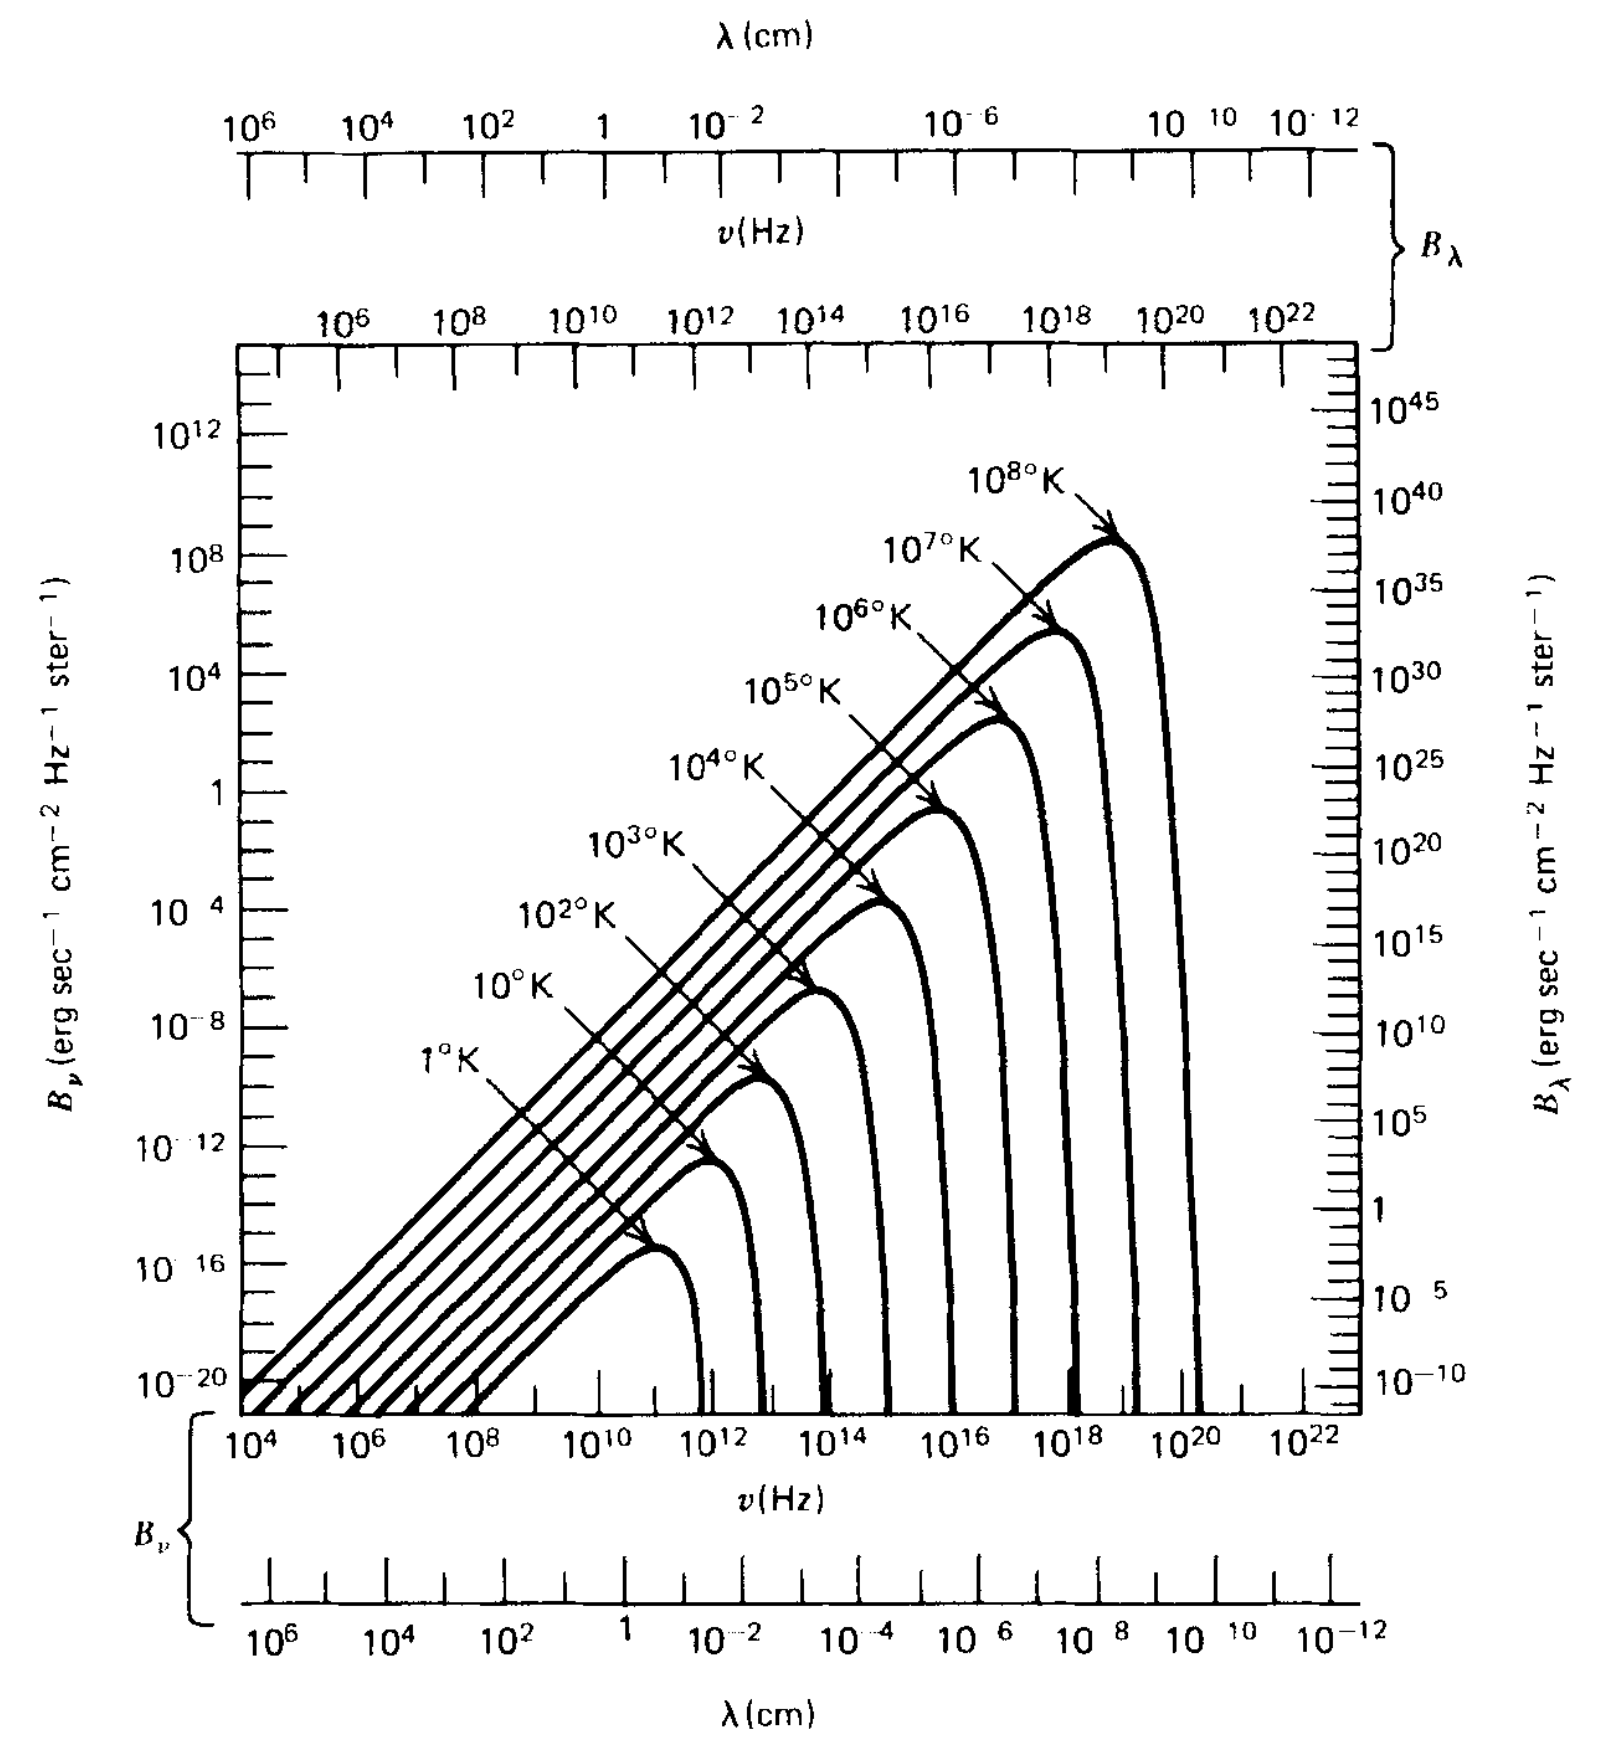
\includegraphics[width=14cm]{figures/cosmology/blackbody.png}
    \centering
    \caption{Blackbody spectra at various temperatures. Figure taken from Ryden (2017).}
    \label{fig:blackbody}
\end{figure}

{\noindent}Figure \ref{fig:blackbody} shows blackbody spectra for various temperatures in log-log space, where the peak of each blackbody spectrum is related to its associated temperature via $h\nu_\mathrm{peak} \approx 2.82\,k_BT$. While the mean photon energy is $2.82\,k_BT$, approximately one in ever 500 photons will have energies exceeding $10\,k_BT$, one in 3 million will exceed $20\,k_BT$, and one in 30 billion will exceed $30\,k_BT$. While only a small fraction of CMB photons are found in the high-energy tail-end of the Planck distribution, the overall number of CMB photons is enormous -- outnumbering baryons by nearly 2 billion to one. Therefore, the vast number of CMB photons surrounding neutral hydrogen atoms greatly increases the probability of photoionization, even with a mean photon energy less than the ionization energy of hydrogen.

\begin{itemize}
    \item Before recombination, photon pressure is preventing collapse -- after recombination this photon pressure is suddenly gone and the Jeans mass drops by a factor of $\approx 10^{10}$ so structure starts growing again.
    \item By the end of recombination, silk damping has removed most of the small scale structure.
\end{itemize}

\subsubsection{Follow-up Questions}

\begin{itemize}
    \item How is the CMB related to recombination?
    \item Around how long ago or at what redshift did this occur?
\end{itemize}

% --------------------------------------------------------------
%
%                           2. 
%
% --------------------------------------------------------------

\newpage
\subsection{Question 2}

The universe is said to be ``flat," or, close to flat. What are the properties of a flat universe and what evidence do we have for it?

\subsubsection{Short answer}

There are three simple properties of a flat Universe: (1) parallel lines never converge nor diverge; (2) the sum of all energy densities is equal to it's critical value; and (3) the sum of angles withing a triangle is always $180^\circ$. Two common techniques for measuring the curvature (i.e., topology) of the Universe include measuring the total energy density of the Universe and using the main peak in the CMB power spectrum as a standard ruler.

\subsubsection{Additional context}

In developing a mathematical theory of general relativity, in which spacetime geometry/curvature is related to the mass-energy density, Einstein needed a way of mathematically describing curvature. Since picturing the curvature of a four-dimensional spacetime is, to say the least, difficult, let's start by considering ways of describing the curvature of two-dimensional spaces, then extend what we have learned to higher dimensions.

{\noindent}The simplest of two-dimensional spaces is a plane, on which Euclidean geometry holds (see (a) of Figure \ref{fig:geometries}). On a plane, a geodesic is a straight line. If a triangle is constructed on a plane by connecting three points with geodesics, the sum of the angles made with its vertices obeys:

\begin{align*}
    \Delta_\mathrm{flat} = \alpha + \beta + \gamma = \pi ~~~~~[{\rm rad}].
\end{align*}

{\noindent}Note that a plane has infinite area, and has no upper limits on the possible distance between points.

{\noindent}Now consider another simple two-dimensional space, the surface of a sphere (see (b) of Figure \ref{fig:geometries}). On the surface of a sphere, a geodesic is a portion of a great circle -- that is, a circle whose center corresponds to the center of the sphere. If a triangle is constructed on the surface of the sphere by connecting three points with geodesics, the sum of the angles made with its vertices obeys:

\begin{align*}
    \Delta_\mathrm{closed} = \alpha + \beta + \gamma = \pi + A/R^2 ~~~~~[{\rm rad}],
\end{align*}

{\noindent}where $A$ is the area of the triangle, and $R$ is the radius of the sphere. All spaces in which $\alpha + \beta + \gamma > \pi$ are called ``positively curved'' spaces. The surface of a sphere is a positively curved two-dimensional space. Moreover, it is a space where the curvature is homogeneous and isotropic; no matter where you draw a triangle on the surface of a sphere, or how you orient it, it must always satisfy the above equation for $\Delta_\mathrm{closed}$. Note that a sphere has a maximum possible distance between points; the distance between antipodal points, at the maximum possible separation, is $\pi R$.

{\noindent}In addition to flat spaces and positively curved spaces, there exist negatively curved spaces. An example of a negatively curved two-dimensional space is the hyperboloid, or saddle-shape (see (c) of Figure \ref{fig:geometries}). If a triangle is constructed on this surface by connecting three points with geodesics, the sum of the angles made with its vertices obeys:

\begin{align*}
    \Delta_\mathrm{open} = \alpha + \beta + \gamma = \pi - A/R^2 ~~~~~[{\rm rad}],
\end{align*}

{\noindent}where $A$ is the area of the triangle, and $R$ is the radius of curvature. All spaces in which $\alpha + \beta + \gamma < \pi$ are called ``negatively curved'' spaces. The surface of a hyperboloid is a negatively curved two-dimensional space. A surface of constant negative curvature has infinite area, and has no upper limit on the possible distance between points.

\begin{figure}[h]
    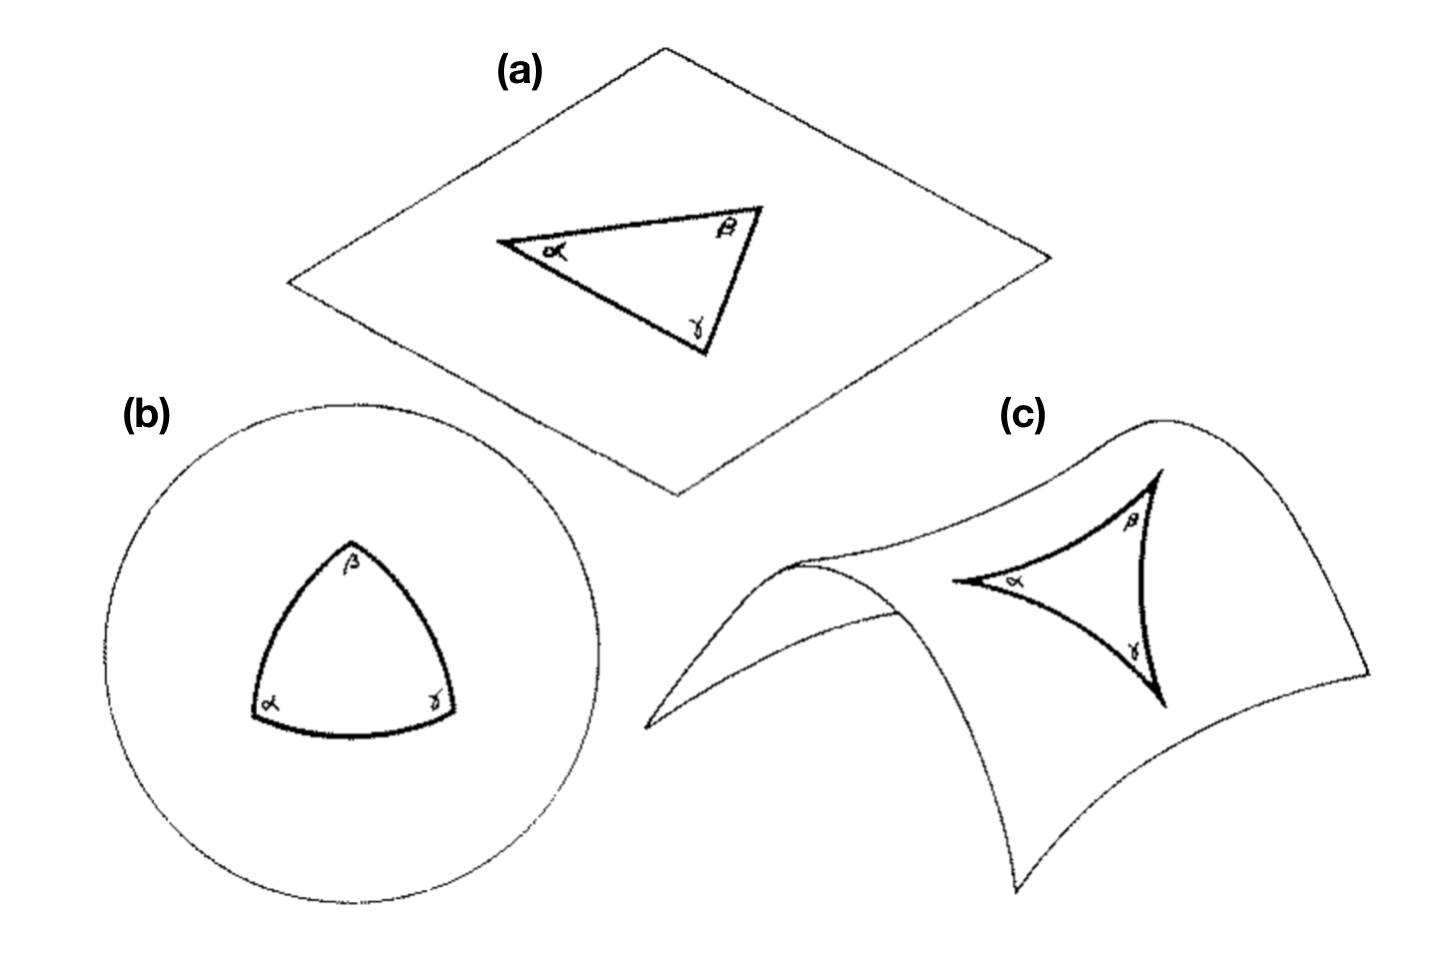
\includegraphics[width=14cm]{figures/cosmology/geometries.png}
    \centering
    \caption{(a) Flat geometry for which $ \Delta_\mathrm{flat} = \alpha + \beta + \gamma = \pi$. (b) Closed geometry for which $\Delta_\mathrm{closed} = \alpha + \beta + \gamma = \pi + A/R^2$, where $A$ is the area of the triangle, and $R$ is the radius of the sphere. (c) Open geometry for which $\Delta_\mathrm{open} = \alpha + \beta + \gamma = \pi - A/R^2$, where $A$ is the area of the triangle, and $R$ is the radius of curvature.}
    \label{fig:geometries}
\end{figure}

{\noindent}If you want a two-dimensional space to be homogeneous and isotropic, there are only three possibilities that fit the bill: the space can be uniformly flat, it can have uniform positive curvature, or it can have uniform negative curvature. Thus, if a two-dimensional space has curvature which is homogeneous and isotropic, its geometry can be specified by two quantities, $\kappa$, and $R$. The number $\kappa$, called the curvature constant, is $\kappa = 0$ for a flat space, $\kappa = +1$ for a positively curved space, and $\kappa = −1$ for a negatively curved space. If the space is curved, then the quantity $R$, which has dimensions of length, is the radius of curvature.

{\noindent}The results for two-dimensional space can be extended straightforwardly to three dimensions. A three-dimensional space, if its curvature is homogeneous and isotropic, must be flat, have uniform positive curvature, or have uniform negative curvature. If a three-dimensional space is flat ($\kappa = 0$), it has the following metric:

\begin{align*}
    ds^2_\mathrm{flat} = dx^2 + dy^2 + dz^2.
\end{align*}

{\noindent}By making the simple coordinate substitution $x = r\cos\theta$, $y = r\sin\theta$, this can be written in spherical coordinates as:

\begin{align*}
    ds^2_\mathrm{flat} = dr^2 + r^2[d\theta^2 + \sin^2\theta d\phi^2].
\end{align*}

{\noindent}If a three-dimensional space has uniform positive curvature ($\kappa = +1$), its metric is

\begin{align*}
    ds_\mathrm{closed}^2 = dr^2 + R^2\sin^2(r/R)[d\theta^2 + \sin^2\theta d\phi^2].
\end{align*}

{\noindent}A positively curved three-dimensional space has finite volume, just as a positively curved two-dimensional space has finite area. The point at $r = \pi R$ is the antipodal point to the origin, just as the south pole, at $r = \pi R$, is the antipodal point to the north pole, at $r = 0$, on the surface of a sphere. By traveling a distance $C = 2\pi R$, it is possible to ``circumnavigate'' a space of uniform positive curvature.

{\noindent}If a three-dimensional space has uniform negative curvature ($\kappa =
−1$), its metric is

\begin{align*}
    ds_\mathrm{open}^2 = dr^2 + R^2\sinh^2(r/R)[d\theta^2 + \sin^2\theta d\phi^2].
\end{align*}

{\noindent}Like flat space, negatively curved space has infinite volume.

{\noindent}The three possible metrics for a homogeneous, isotropic, three-dimensional
space can be written more compactly in the form:

\begin{align*}
    ds^2 = dr^2 + S_\kappa(r)^2d\Omega^2
\end{align*}

{\noindent}where

\begin{align*}
    d\Omega \equiv d\theta^2 + \sin^2\theta d\phi^2
\end{align*}

{\noindent}and

\begin{equation*}
    S_\kappa(r) =
    \left\{
    \begin{aligned}
    R\sin(r/R), ~~~~~& (\kappa = +1) \\
              r,~~~~~& (\kappa = 0) \\
    R\sinh(r/R),~~~~~& (\kappa = -1)
    \end{aligned}
    \right.
    .
\end{equation*}

{\noindent}The coordinate system ($r,\theta,\phi$) is not the only possible system. For instance, if we switch the radial coordinate from $r$ to $x \equiv S_\kappa(r)$, the metric for a homogeneous, isotropic, three-dimensional space can be written in the form:

\begin{align*}
    ds^2 = \frac{dx^2}{1-\kappa x^2/R^2} + x^2d\Omega^2.
\end{align*}

The \textbf{critical density} of the Universe is defined to be

\begin{align*}
    \rho_c \equiv \left( \frac{3H_0}{8\pi G} \right) ~ [{\rm g\,cm^{-3}}].
\end{align*}

{\noindent}If the total energy density is higher than this, then the Universe is said to be \textbf{closed}: initially parallel lines eventually converge, just as lines of constant longitude meet at the North and South poles. A closed Universe, much like the surface of a sphere, has positive curvature. In a low-density Universe whose total energy density is less than critical value, the Universe is said to be \textbf{open}: initially parallel lines eventually diverge, as would marbles rolling off a saddle. While a closed Universe has positive curvature, an open Universe has negative curvature.

% --------------------------------------------------------------
%
%                           3. 
%
% --------------------------------------------------------------

\newpage
\subsection{Question 3}

Outline the development of the Cold Dark Matter spectrum of density fluctuations from the early universe to the current epoch.

\subsubsection{Short answer}

Answer.

\subsubsection{Additional context}

The generally accepted theoretical framework for the formation of structure is that of gravitational instability. The gravitational instability scenario assumes that the early universe was almost perfectly smooth, with the exception of tiny density perturbations with respect to the global cosmic background density and the accompanying tiny velocity perturbations from the general Hubble expansion. The observed fluctuations in the CMB temperature are a reflection of these density perturbations, so we know that the primordial density perturbations must have been on the order of $\Delta T / T \sim 10^{-5}$. The origin of this density perturbation field has yet to be fully understood, but the most plausible theory currently is that they are a result of \textit{quantum fluctuations} which, during the inflationary phase, expanded to macroscopic scales.

{\noindent}Originally minute deviations from the average density of the Universe, and the corresponding deviations from the global cosmic expansion velocity (i.e., the Hubble expansion), will start to grow under the influence of gravity where the density perturbations will have induced local differences in gravity. During its early evolution, an overdensity will experience a gradually stronger deceleration of its expansion velocity such that its expansion velocity will continue to slow down with respect to the Hubble expansion. Since matter is gravitationally attracted to regions of higher density, it will also have the tendency to move towards that region. When the region has become sufficiently overdense, the mass of the density perturbation will have grown so much that its expansion would come to a halt. The region then completely decouples from the Hubble expansion and begins to collapse under its own gravity. The newly formed gravitationally bound object will reach virial equilibrium at which point it becomes a recognizable comic object; its precise nature (e.g., galaxy, cluster etc.) being determined by the properties of the initial density perturbation and its surroundings.

{\noindent}The opposite tendency will have occurred for underdensities in the matter density field. Since they contain less matter than the average density field, its expansion deceleration is less than the Hubble expansion which results in matter becoming even more dispersed and underdensities continuing to expand. As this process continues and becomes more pronounced, such underdensities result in the gradual emergence of voids in the matter distribution of the Universe. The most dramatic evidence for these spatial nonuniformities (i.e., overdensities and voids) on the largest of scales comes from redshift surveys such as the 2dF Galactic Redshift Survey\footnote{\href{http://www.2dfgrs.net/}{2dFGRS: http://www.2dfgrs.net/}} shown in Figure \ref{fig:2df}.

\begin{figure}[h]
    \floatbox[{\capbeside\thisfloatsetup{capbesideposition={right,top},capbesidewidth=4cm}}]{figure}[\FBwidth]
    {\caption{\footnotesize{The spatial distribution of galaxies in two four-degree strips on the sky, according to the 2dF Galaxy Redshift Survey. Note the $100\,{\rm Mpc}$ filamentary features and the prominent voids. One of the principal challenges in cosmology is to explain this pattern, which is most probably a relic of the very earliest stages of the expanding Universe. Figure taken from Ryden (2017).}}
    \label{fig:2df}}
    {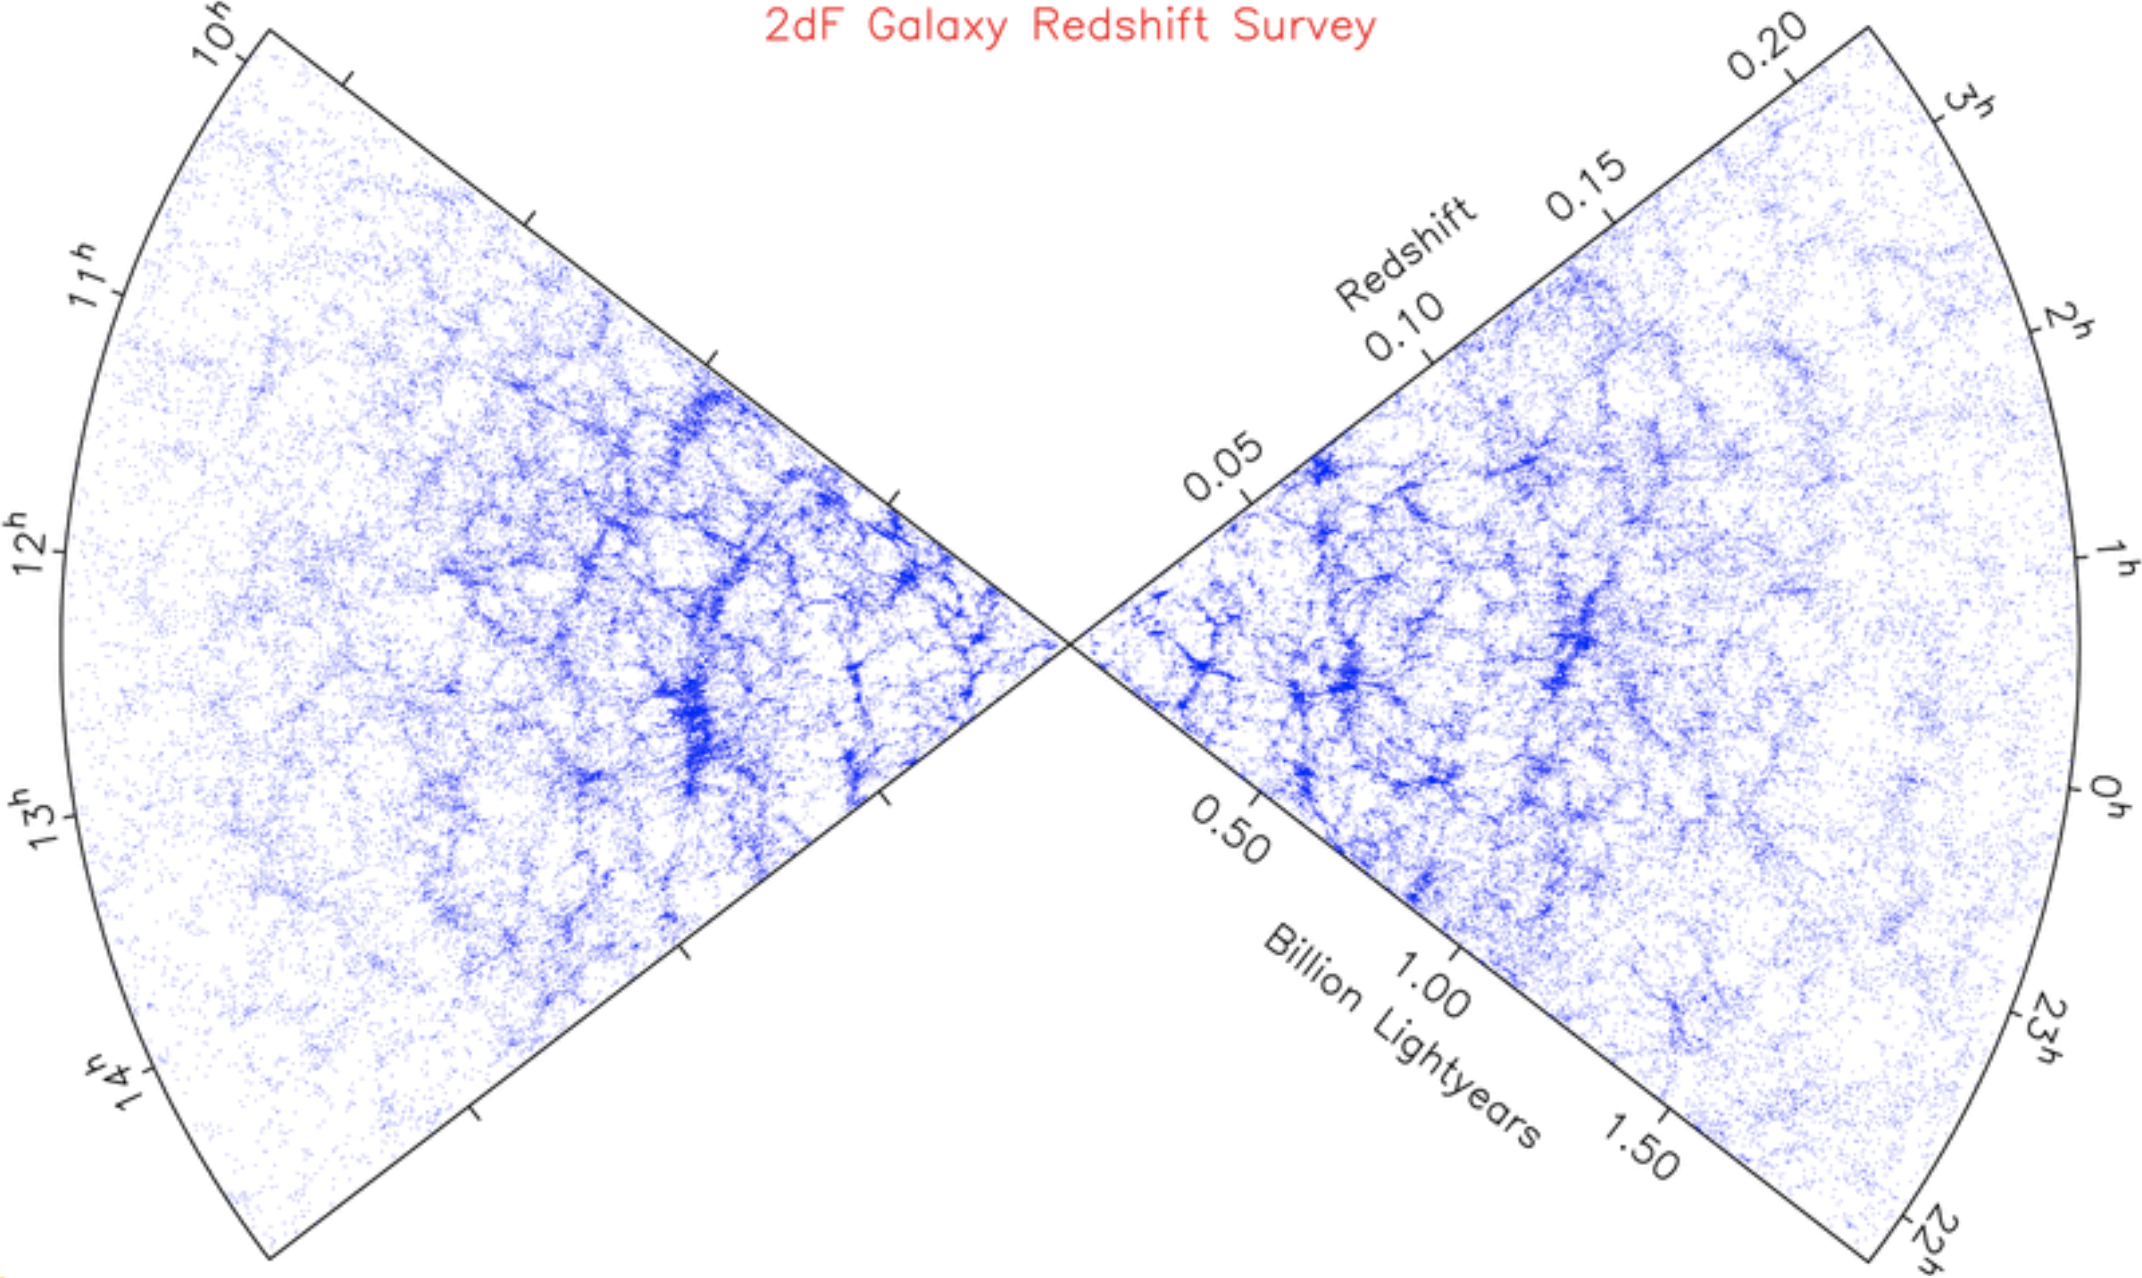
\includegraphics[width=10cm]{figures/cosmology/2df.png}}
\end{figure}

{\noindent}Galaxies in Figure \ref{fig:2df} are clearly not distributed randomly: the Universe has structure on large scales. To understand this structure, we must go beyond the Standard Model not only by including dark matter, but also by allowing for deviations from smoothness. We must develop the tools to study perturbations around the smooth background of the Standard Model. This is straightforward in theory, as long as the perturbations remain small (i.e., linear). Indeed, understanding the development of structure in the universe has become a major goal of most cosmologists today. Dark matter is needed not only to explain rotation curves of galaxies but to explain structure in the Universe at large!

{\noindent}The best ways to learn about the evolution of structure and to compare theory with observations are to look at anisotropies in the CMB and at how matter is distributed on large scales. Anisotropies in the CMB today tell us what the Universe looked like when it was several hundred thousand years old, so they are wonderful probes of the perturbations. To compare theory with observations, we must at first try to avoid scales dominated by nonlinearities. As an extreme example, we can never hope to understand cosmology by carefully examining rock formations on Earth. The intermediate steps -- collapse of matter into a galaxy; molecular cooling; star formation; planetary formation; etc. -- are much too complicated to allow comparison between linear theory and observations. While perturbations to matter on small scales (less than about $100\,{\rm Mpc}$) have grown nonlinear, large-scale perturbations are still small so they have been processed much less than the corresponding small-scale structure. Similarly, anisotropies in the CMB have remained small because the photons that make up the CMB do not clump.

{\noindent}Identifying large-scale structure and the CMB as the two most promising areas of study solves just one issue. Another very important challenge is to understand how to characterize these distributions so that theory can be compared to experiment. It is one thing to look at a map and quite another to quantitatively test cosmological models. To make such tests, it is often useful to take the Fourier transform of the distribution in question; as we will see, working in Fourier space makes it easier to separate large from small scales. The most important statistic in the cases of both the CMB and large-scale structure is the \textbf{two-point correlation function}, called the \textbf{power spectrum} in Fourier space.

{\noindent}If the mean density of galaxies at some time $t$ is $\langle\rho(t)\rangle$, then we can characterize the inhomogeneities with the dimensionless \textbf{density perturbation field} (also known as the \textbf{density contrast}) which is used to relate the energy density $\rho(\mathbf{x},t)$ at some co-moving spatial coordinate $\mathbf{x}$ and time $t$ to the average energy density at that time $\langle\rho(t)\rangle$:

\begin{align*}
    \delta(\mathbf{x},t) \equiv \frac{\rho(\mathbf{x},t)~- \langle\rho(t)\rangle}{\langle\rho(t)\rangle} ~ [{\rm dimensionless}].
\end{align*}

{\noindent}Evidently, in an unperturbed Universe with $\rho(\mathbf{x},t) = \langle\rho(t)\rangle$ everywhere, $\delta(\mathbf{x},t) = 0$. Note that positive density fluctuations (i.e., overdensities) may in principle grow limitless whereas negative density fluctuations (i.e., underdensities) have a strict lower-limit of $\delta \geq -1$ (emptier than empty simply doesn't exist). In a complete description of density perturbations, the total energy density of the Universe includes components of baryonic matter ($\rho_b$), cold dark matter ($\rho_c$), radiation ($\rho_\mathrm{rad}$), and dark energy ($\rho_\Lambda$):

\begin{align*}
    \rho(\mathbf{x},t) = \rho_b(\mathbf{x},t) + \rho_c(\mathbf{x},t) + \rho_\mathrm{rad}(\mathbf{x},t) + \rho_\Lambda(\mathbf{x},t) ~ [{\rm g\,cm^{-3}}].
\end{align*}

{\noindent}In terms of their global gravitational influence, dark matter and baryonic matter contribute and evolve equivalently, therefore on cosmological scales they can be combined into a total matter energy density $\rho_m = \rho_b + \rho_c$. Each component may have its own (primordial) perturbation character. Dark energy does not have any density fluctuations, so $\delta_\Lambda(\mathbf{x},t) = 0$. Since most of the structure formation happened during the \textit{matter-dominated era}, this mainly involves the evolution of matter linear perturbations $\delta_m(\mathbf{x},t)$.

{\noindent}In addition to the density contrast, an alternative (and equivalent) description of the statistical properties of the matter distribution in the Universe is the \textbf{power spectrum} $P(k)$. Roughly speaking, the power spectrum describes the level of structure as a function of the length scale $L \simeq 2\pi/k$ where $k$ is a co-moving wavenumber. Phrased differently, the density fluctuations are decomposed into a set of plane waves of the form $\delta(\mathbf{x}) = \sum a_k\cos(\mathbf{x\cdot k})$ with wave vector $\mathbf{k}$ and amplitude $a_k$. The power spectrum $P(k)$ then describes the mean of the squares of the amplitudes $\lvert a_k \rvert^2$ averaged over all wave vectors with equal length $\lvert\mathbf{k}\rvert = k$. Technically speaking, this is a Fourier decomposition. The Fourier transform of $\delta(\mathbf{x},t)$ is $\tilde{\delta}(\mathbf{x},t)$, which allows the power spectrum $P(k)$ to be defined via

\begin{align*}
    \langle \tilde{\delta}(\mathbf{k}) \tilde{\delta}(\mathbf{k'}) \rangle = (2\pi)^3 P(k) \delta^3 (\mathbf{k} - \mathbf{k'}),
\end{align*}

{\noindent}where the angular brackets denote averaging over the entire distribution, $k$ is the wavenumber, and $\delta^3()$ is the delta Dirac function which constrains $\mathbf{k}=\mathbf{k'}$. This indicates that the power spectrum is the spread, or the variance, in the distribution. Figure \ref{fig:galaxypowerspec} shows the combination $k^3P(k)/2\pi^2$, a dimensionless number which is a good indication of the clumpiness on scale $k$.

{\noindent}The power spectrum $P(k)$ and the two-point correlation function $\xi(x)$ are related through the Fourier transform as

\begin{align*}
    P(k) = 2\pi \int\limits_0^\infty \frac{\sin(kx)}{kx} x^2 \xi(x)\,{\rm d}x,
\end{align*}

{\noindent}i.e., the integral over the correlation function with a weight factor depending on the wave number provides the power spectrum. This relation can also be inverted to obtain the inverse Fourier transform such that the correlation function can be computed from the power spectrum. In general, knowing the power spectrum is insufficient to unambiguously describe the statistical properties of any density field; as such, the power spectrum is often used alongside the correlation function $\xi(x)$. Given observation data, either the power spectrum or the correlation function may be easier to compute, or another may be easier to obtain from models or simulations. In addition, our intuitive understanding of these functions may vary in different situations.

\begin{figure}[t]
    \floatbox[{\capbeside\thisfloatsetup{capbesideposition={right,top},capbesidewidth=4cm}}]{figure}[\FBwidth]
    {\caption{\footnotesize{The variance $\Delta^2 \equiv k^3P(k)/2\pi^2$ of the Fourier transform of the galaxy distribution as a function of scale. On large scales, the variance is smaller than unity so the distribution is smooth. The solid line is the theoretical model in which the Universe contains dark matter and a cosmological constant with perturbations generated by inflation. The dashed line is a model with only baryons and no dark matter. Data came from the PSCz survey (Saunders et ai, 2000) as analyzed by Hamilton and Tegmark (2001). Figure from Ryden (2017).}}
    \label{fig:galaxypowerspec}}
    {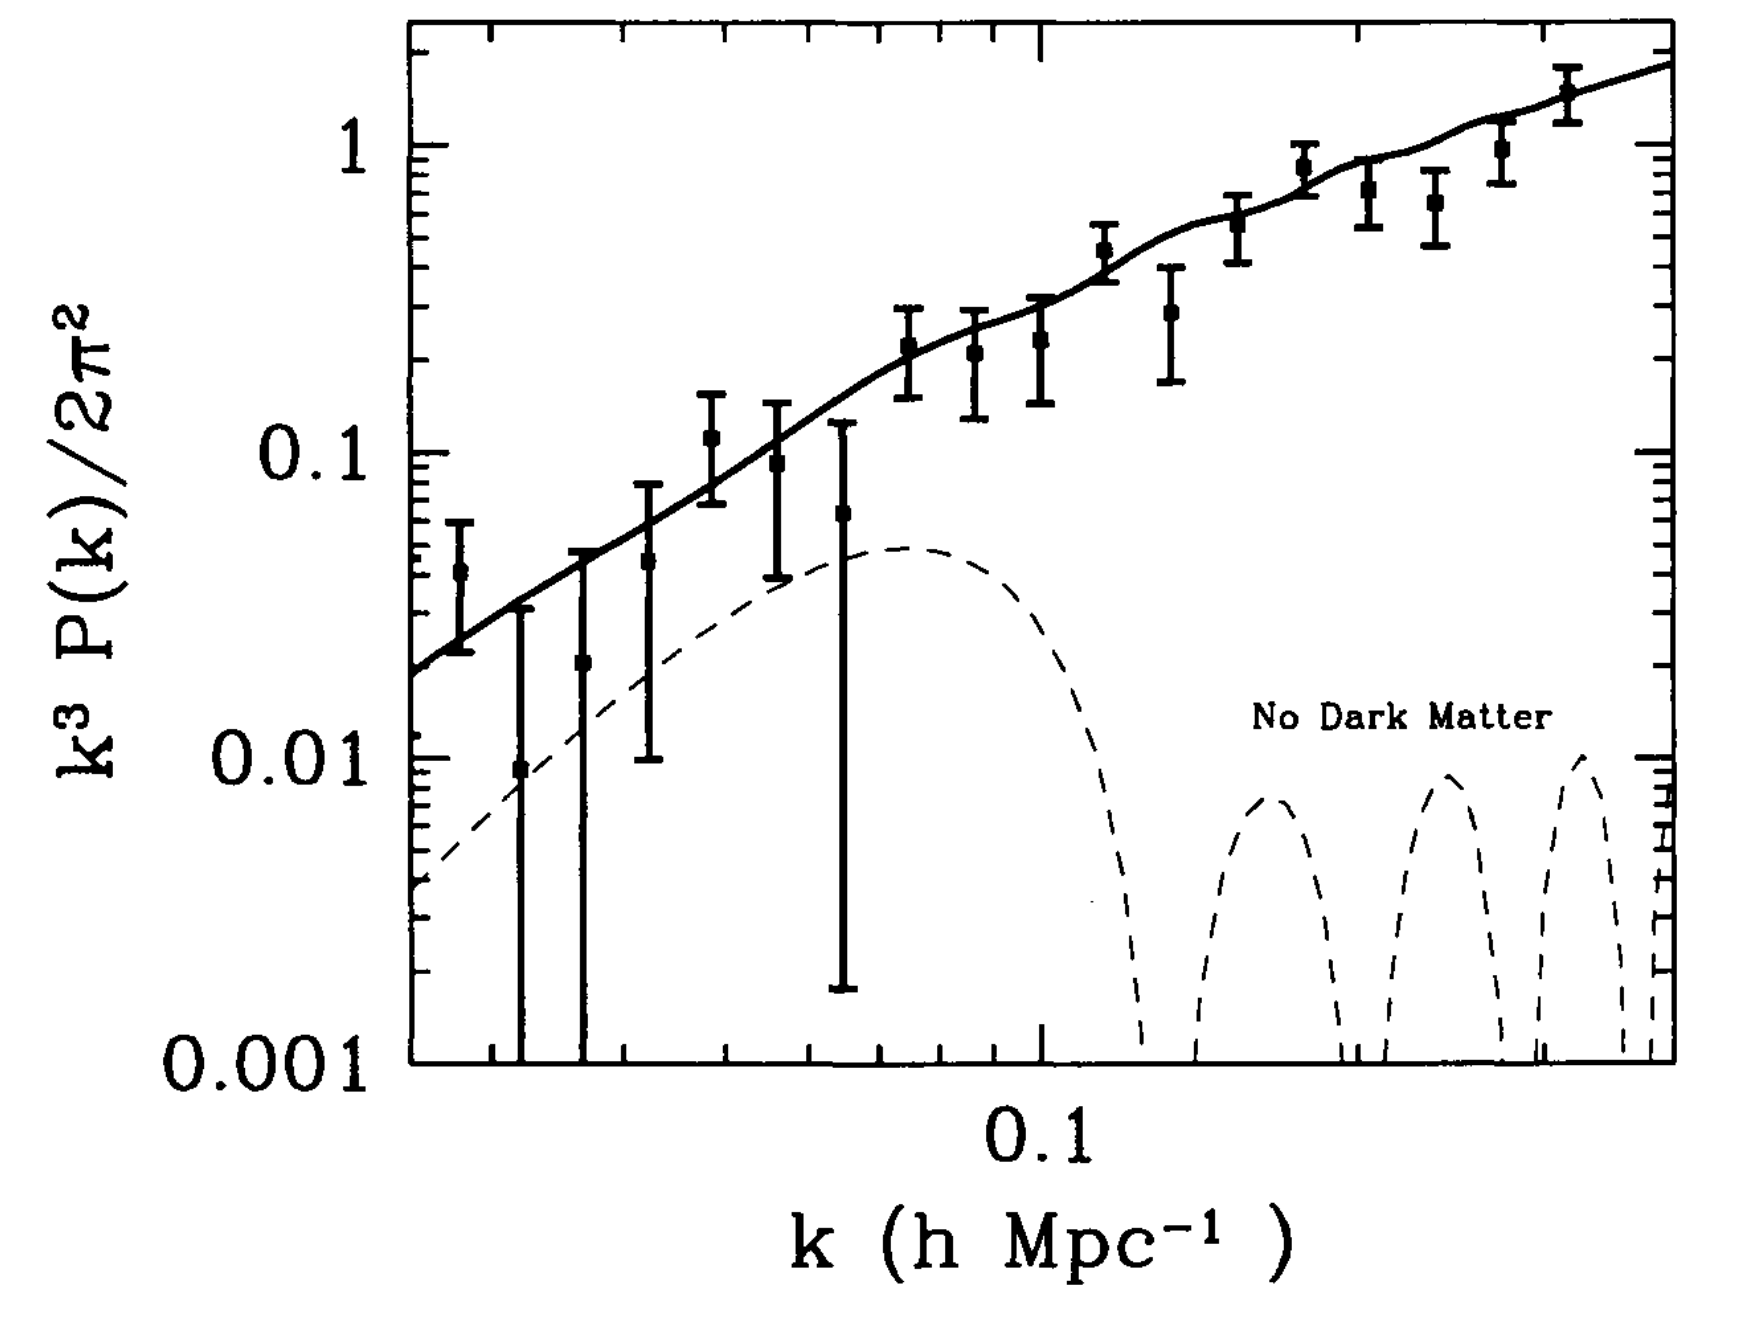
\includegraphics[width=12cm]{figures/cosmology/GalaxyPowerSpectrum.png}}
\end{figure}

\begin{figure}[h]
    \floatbox[{\capbeside\thisfloatsetup{capbesideposition={right,top},capbesidewidth=4cm}}]{figure}[\FBwidth]
    {\caption{\footnotesize{Anisotropies in the CMB predicted by the theory of inflation compared with observations, x-axis is multipole moment (e.g., $\ell = 1$ is the dipole, $\ell = 2$ the quadrupole) so that large angular scales correspond to low $\ell$; y-axis is the root mean square anisotropy (the square root of the two-point correlation function) as a function of scale. The characteristic signature of inflation is the series of peaks and troughs, a signature which has been verified by experiment. Figure from Ryden (2017).}}
    \label{fig:cmbpowerspec}}
    {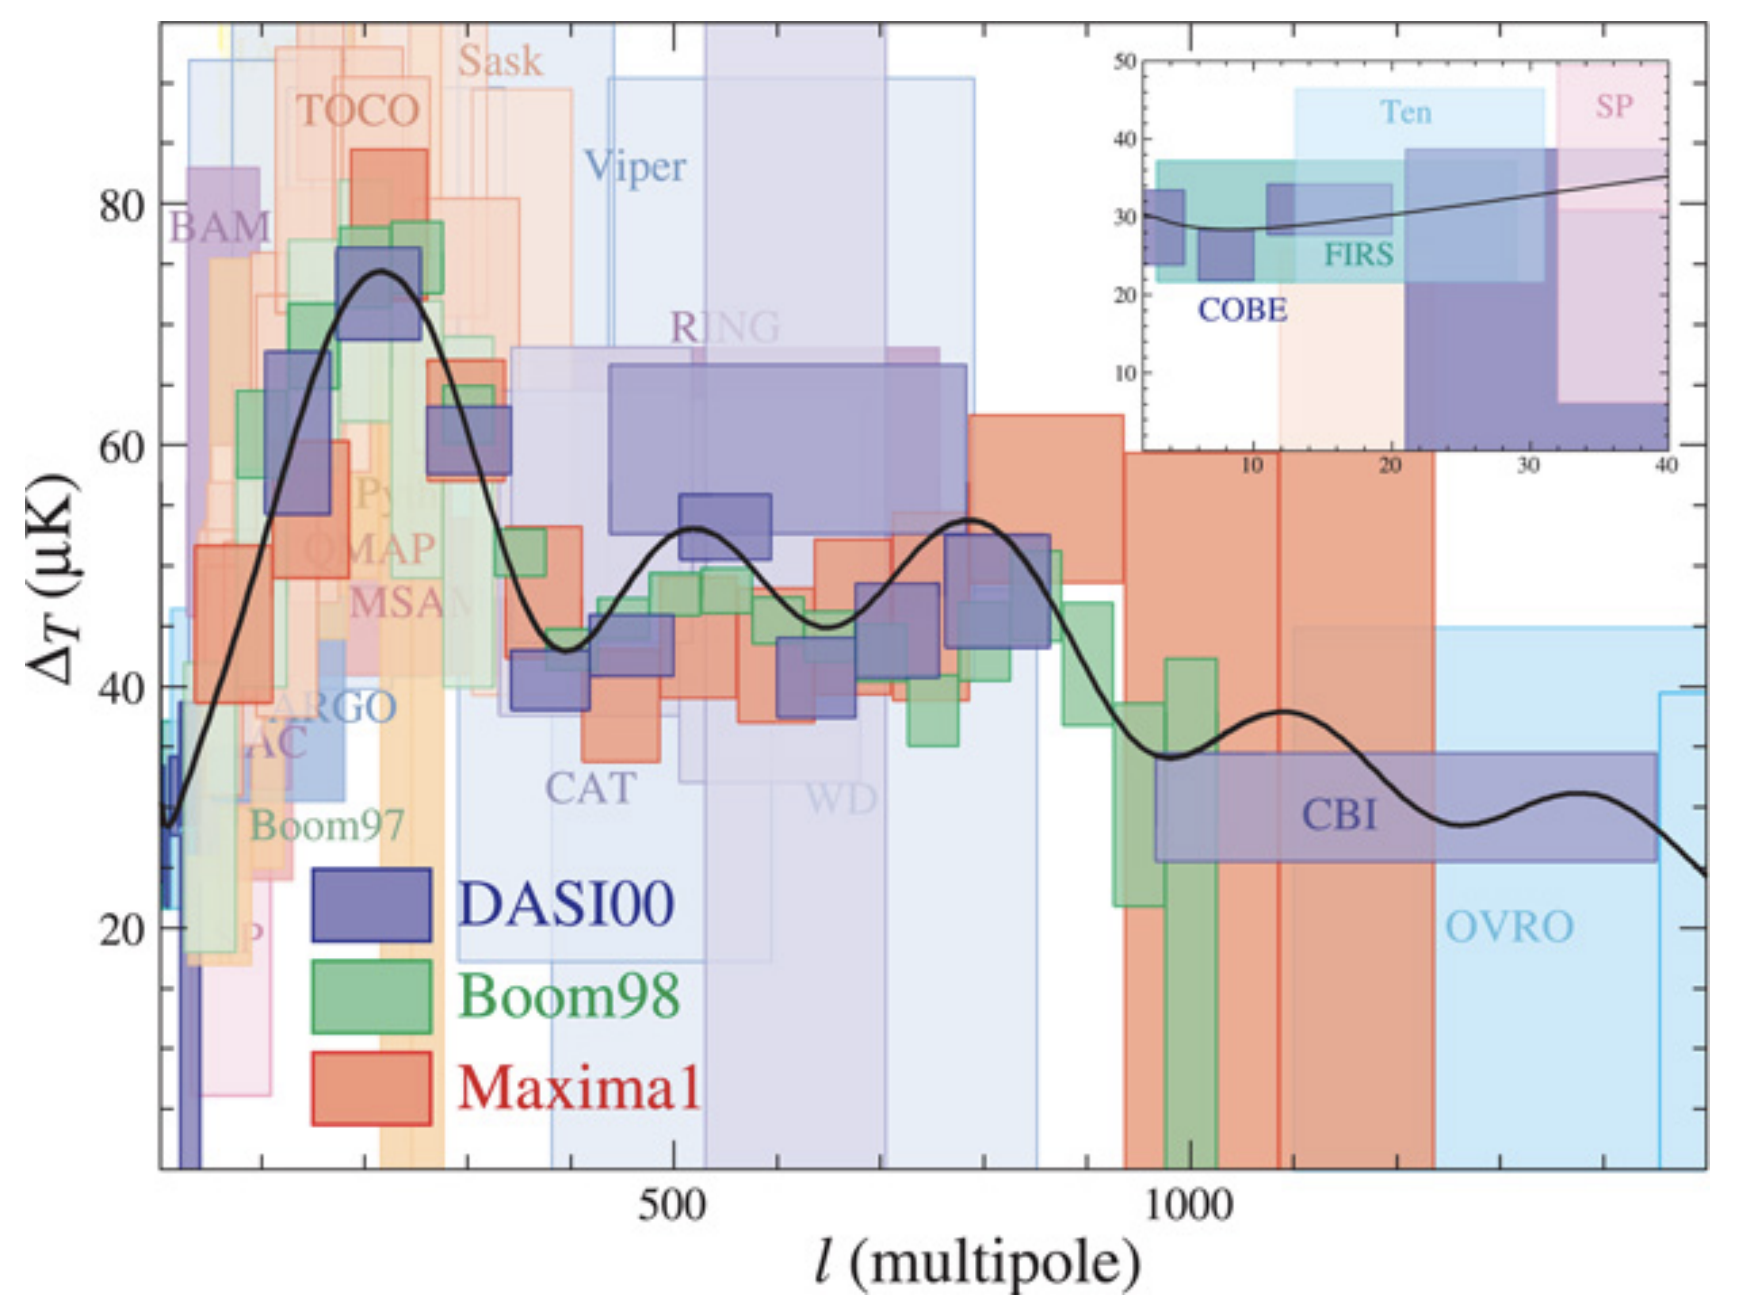
\includegraphics[width=12cm]{figures/cosmology/CMBPowerSpectrum.png}}
\end{figure}

{\noindent}The best measure of anisotropies in the CMB is also the two-point correlation function of the temperature distribution. There is a subtle technical difference between the two power spectra which are used to measure the galaxy distribution and the CMB, though. The difference arises because the CMB temperature is a two-dimensional field, measured everywhere on the sky (i.e., with two angular coordinates). Instead of Fourier transforming the CMB temperature, then, one typically expands it in spherical harmonics, a basis more appropriate for a 2D field on the surface of a sphere. Therefore the two-point correlation function of the CMB is a function of multipole moment $\ell$, not wave number $k$. Figure \ref{fig:cmbpowerspec} shows the measurements of dozens of groups since 1992, when COBE first discovered large-angle (low $\ell$ in the plot) anisotropies.

{\noindent}It is assumed that in very early epochs, the matter density field obeyed Gaussian statistics. This is a prediction of a large class of inflationary models which are supposed to generate the primordial density fluctuations of the Universe. An important property of Gaussian statistics, or \textit{Gaussian random fields}, is that their distributions are uniquely determined by their power spectrum $P(k)$. Among the properties which characterize these Gaussian random fields, the probability distribution of the density fluctuations $\delta(\mathbf{x})$ at any point is a Gaussian distribution. Observational evidence for the Gaussian nature of the early density fluctuations comes from observations of anisotropies in the CMB which very strongly constrain any possible deviation from a Gaussian random field in the early Universe.

{\noindent}The early linear stages of structure formation have been successfully and completely worked out within the context of \textit{linear perturbation theory}. For this discussion of the growth of density perturbations, we are concentrating on length scales that are substantially smaller than the Hubble radius. On such scales, structure growth can be described in the framework of the Newtonian theory of gravity; the effects of spacetime curvature and thus General Relativity need only be accounted for when density perturbations are on length scales comparable to, or larger than, the Hubble radius. In addition, we assume for simplicity that the matter in the Universe consists of only pressure-free matter described in the \textit{fluid approximation}.

{\noindent}Approximate solutions of the set of equations which describe small deviations from the homogeneous solution have the form

\begin{align*}
    \delta(\mathbf{x},t)=D(t)\tilde{\delta}(\mathbf{x}),
\end{align*}

{\noindent}i.e., the spatial and temporal dependencies factorize in these solutions. Here, $\tilde{\delta}(\mathbf{x})$ is an arbitrary function of the spatial coordinate, and D(t) satisfies the equation

\begin{align*}
    \ddot{D}(t)+\frac{2\dot{a}}{a}\dot{D}(t)-4\pi G\bar{\rho}(t)D(t) = 0.
\end{align*}

{\noindent}The differential equation has two linearly independent solutions. One can show that one of them increases with time, whereas the other decreases. If, at some early time, both functional dependencies were present, the increasing solution will dominate at later times, whereas the solution decreasing with $t$ will become irrelevant. Therefore, we will consider only the increasing solution, which is denoted by $D_+(t)$, and normalize it such that $D_+(t_0)=1$. Then, the density contrast becomes

\begin{align*}
    \delta(\mathbf{x},t) = D_+(t)\delta_0(\mathbf{x}).
\end{align*}

{\noindent}This mathematical consideration allows us to draw immediately a number of conclusions. First, the solution implies that in linear perturbation theory the spatial shape of the density fluctuations is frozen in comoving coordinates, only their amplitude increases. The growth factor $D_+(t)$ of the amplitude follows a simple differential equation that is readily solvable for any cosmological model. In fact, one can show that for arbitrary values of the density parameters in matter and vacuum energy, the growth factor has the form

\begin{align*}
    D_+(t) \propto \frac{H(a)}{H_0}\int\limits_0^a \frac{da'}{[\Omega_m/a'+\Omega_\Lambda a'^2-(\Omega_m+\Omega_\Lambda-1)]^{3/2}},
\end{align*}

{\noindent}where the factor of proportionality is determined from the condition $D_+(t_0)=1$.

{\noindent}Primordial density perturbations on a small scale appear to have a much higher amplitude than those on larger scales. This leads to a hierarchical process of structure formation, with small-scale perturbations being the first one to become nonlinear and develop into cosmic objects.

{\noindent}Returning to the two-point correlation function and Fourier transform, $P(k)$ and $\xi(x)$ both depend on cosmological time or redshift because the density field in the Universe evolves over time. Therefore, the dependence on $t$ is explicitly written as $P(k,t)$ and $\xi(x,t)$. Note that $P(k,t)$ is linearly related to $\xi(x,t)$ and $\xi(x,t)$ in turn depends quadratically on the density contrast $\delta$. If $x$ is the comoving separation vector, we then know the time dependence of the density fluctuations, $\delta(x,t)=D_+(t)\delta_0(\mathbf{x})$. Thus,

\begin{align*}
    \xi(x,t) = D_+^2(t)\xi(x,t_0),
\end{align*}

{\noindent}and accordingly,

\begin{align*}
    P(k,t) = D_+^2(t)P(k,t_0) \equiv D_+^2(t)P_0(k),
\end{align*}

{\noindent}We stress that these relations are valid only in the framework of Newtonian, linear perturbation theory in the matter dominated era of the Universe. This last equation states that the knowledge of $P_0(k)$ is sufficient to obtain the power spectrum $P(k,t)$ at any time, again within the framework of linear perturbation theory.

{\noindent}Initially it may seem as if $P_0(k)$ is a function that can be chosen arbitrarily, but one objective of cosmology is to calculate this power spectrum and to compare it to observations. More than 30 years ago, arguments were already developed to specify the functional form of the initial power spectrum.

{\noindent}At early times, the expansion of the Universe follows a power law, $a(t)\propto t^{1/2}$ in the radiation-dominated era. At that time, no natural length-scale existed in the Universe to which one might compare a wavelength. The only mathematical function that depends on a length but does not contain any characteristic scale is a power law; hence for very early times one should expect

\begin{align*}
    P(k) \propto k^{n_s}.
\end{align*}

{\noindent}Many years ago, Harrison, Zeldovich, Peebles and others argued that $n_s=1$, as for this slope, the amplitude of the fluctuations of the gravitational potential are constant (i.e., preferring neither small nor large scales). For this reason, this spectrum with $n_s=1$ is called a scale-invariant spectrum, or Harrison-Zeldovich spectrum. With such a spectrum, we may choose a time $t_i$ after the inflationary epoch and write

\begin{align*}
    P(k,t_i) = D_+^2(t_i)Ak^{n_s},
\end{align*}

{\noindent}where $A$ is a normalization constant that cannot be determined from theory but has to be fixed by observations. However, this is not the complete story: the result needs to be modified to account for the different growth of the amplitude of density fluctuations in the radiation-dominated epoch of the Universe, compared to that in the later cosmic epochs from which our result was derived.

{\noindent}Furthermore, these modifications depend on the nature of the dark matter. One distinguishes between cold dark matter (CDM) and hot dark matter (HDM). These two kinds of dark matter differ in the characteristic velocities of their constituents. Cold dark matter has a velocity dispersion that is negligible compared to astrophysically relevant velocities (e.g., the virial velocities of low-mass dark matter halos). Therefore, their initial velocity dispersion can well be approximated by zero, and all dark matter particles have the bulk velocity of the cosmic `fluid' (before the occurrence of multiple streams). In contrast, the velocity dispersion of hot dark matter is appreciable; neutrinos are the best candidates for HDM, in view of their known abundance, determined from the thermal history of the Universe, and their finite rest mass. The characteristic velocity of neutrinos is fully specified by their rest mass; despite their low temperature of $T_\nu=1.9\,{\rm K}$ today, their thermal velocities of

\begin{align*}
    v_\nu \sim 150(1+z)\left(\frac{m_\nu}{1\,{\rm eV}}\right)^{-1} ~ [{\rm km\,s^{-1}}]
\end{align*}

{\noindent}prevent them from forming matter concentrations at all mass scales except for the most massive ones, as their velocity is larger than the corresponding escape velocities. In other words, the finite velocity dispersion of HDM is equivalent to assigning to it a pressure, which prevents them to fall into shallow gravitational potential wells. We will see below the dramatic differences between these two kinds of dark matter for the formation of structures in the Universe. In particular, this estimate shows that neutrinos cannot account for the dark matter on galaxy scales, and thus cannot explain the flat rotation curves of spiral galaxies.

{\noindent}If density fluctuations become too large on a certain scale, linear perturbation theory breaks down and the linear approximation to the solution of $P(k,t)$ is no longer valid. Then the true current-day power spectrum $P(k,t_0)$ will deviate from $P_0(t)$. Nevertheless, in this case it is still useful to examine $P_0(t)$ -- it is then called the linearly extrapolated power spectrum.

{\noindent}Within the framework of linear Newtonian perturbation theory in the `cosmic fluid', $\delta(\mathbf{x},t) = D_+(t)\delta(\mathbf{x})$ applies. Modifications to this behavior are necessary for several reasons:

\begin{itemize}
    \item If dark matter consists (partly) of HDM, this may not be gravitationally bound to the potential well of a density concentration. In this case, the particles are able to move freely and to escape from the potential well, which in the end leads to its dissolution if these particles dominate the matter overdensity. From this argument, it follows immediately that for HDM, small-scale density perturbations cannot form. For CDM this effect of free streaming does not occur.
    \item At redshifts $z\gtrsim z_\mathrm{eq}$, radiation dominates the density of the Universe. Since the expansion law $a(t)$ is then distinctly different from that in the matter-dominated phase, the growth rate for density fluctuations will also change.
    \item A cosmic horizon exists with comoving scale $r_\mathrm{H,com}(t)$. Physical interactions can take place only on scales smaller than $r_\mathrm{H,com}(t)$. For fluctuations of length-scales $L\sim2\pi/k\gtrsim r_\mathrm{H,com}(t)$, Newtonian perturbation theory will cease to be valid, and one needs to apply linear perturbation theory in the framework of the General Relativity.
\end{itemize}

{\noindent}These effects together will lead to a modification of the shape of the power spectrum, relative to the relation $P(k,t_i)=D_+^2(t_i)Ak^{n_s}$; for example, the evolution of perturbations in the radiation-dominated cosmos proceeds differently from that in the matter-dominated era. The power spectrum $P(k)$ is affected by the combination of the above effects, and will be different from the primordial spectral shape, $P\propto k^{n_s}$. The modification of the power spectrum is described in terms of the transfer function $T(k)$ in the form

\begin{align*}
    P(k,t) = D_+^2(t) Ak^{n_s}T^2(k).
\end{align*}

{\noindent}The transfer function can be computed for any cosmological model if the matter content of the universe is specified. In particular, $T(k)$ depends on the nature of dark matter.

{\noindent}The first of the above points immediately implies that a clear difference must exist between HDM and CDM models regarding structure formation and evolution. In HDM models, small-scale fluctuations are washed out by free-streaming of relativistic particles (i.e., the power spectrum is completely suppressed for large $k$, which is expressed by the transfer function $T(k)$ decreasing exponentially for large $k$). In the context of such a theory, very large structures will form first, and galaxies can form only later by fragmentation of large structures. However, this formation scenario is in clear contradiction with observations. For example, we observe galaxies and QSOs at $z>6$ so that small-scale structure is already present at times when the Universe had less than 10\% of its current age. In addition, the observed correlation function of galaxies, both in the local Universe (see Figure \ref{fig:densitycontrast}) and at higher redshift, is incompatible with cosmological models in which the dark matter is composed mainly of HDM. Therefore we can exclude HDM as the dominant constituent of dark matter. For this reason, it is now commonly assumed that the dark matter is ‘cold’. The achievements of the CDM scenario in the comparison between model predictions and observations fully justify this assumption.

\begin{figure}[t]
    \floatbox[{\capbeside\thisfloatsetup{capbesideposition={right,center},capbesidewidth=4cm}}]{figure}[\FBwidth]
    {\caption{\footnotesize{A density perturbation that enters the horizon during the radiation-dominated epoch of the Universe ceases to grow until matter starts to dominate the energy content of the Universe. In comparison to a perturbation that enters the horizon later, during the matter-dominated epoch, the amplitude of the smaller perturbation is suppressed by a factor $(a_\mathrm{enter}/a_\mathrm{eq})^2$, which explains the qualitative behavior of the transfer function. Adapted from: M. Bartelmann \& P. Schneider 2001, Weak Gravitational Lensing, Phys. Rep. 340, 291. Image taken from Schneider (2006).}}
    \label{fig:densitycontrast}}
    {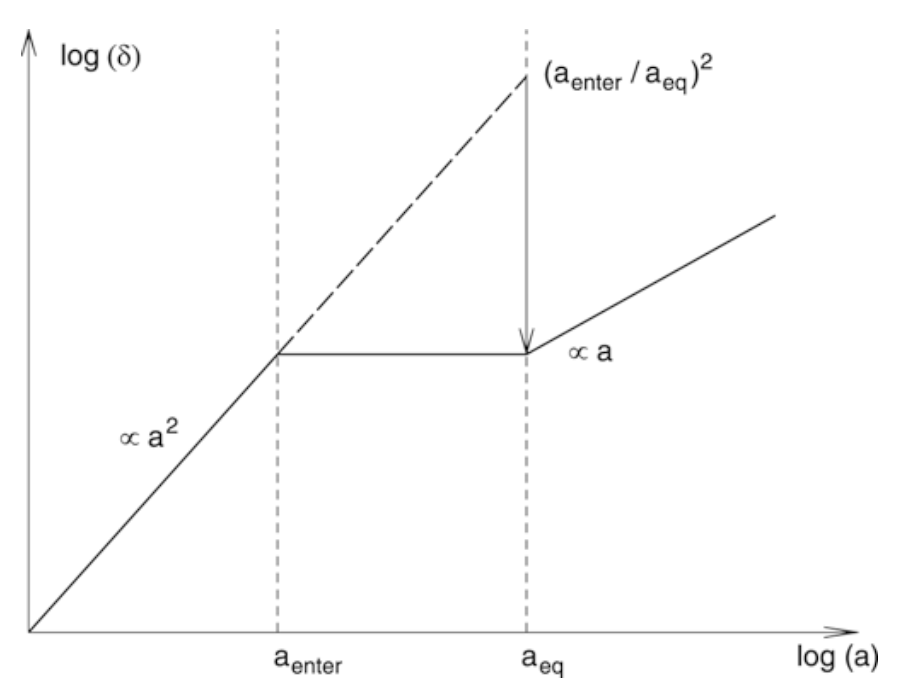
\includegraphics[width=10cm]{figures/cosmology/DensityContrast.png}}
\end{figure}

{\noindent}In linear perturbation theory, fluctuations grow at the same rate on all scales, or for all wave numbers, independent of each other. This applies not only in the Newtonian case, but also remains valid in the framework of General Relativity as long as the fluctuation amplitudes are small. Therefore, the behavior on any (comoving) length-scale can be investigated independently of the other scales. At very early times, perturbations with a comoving scale $L$ are larger than the (comoving) horizon, and only for $z<z_\mathrm{enter}(L)$ does the horizon become larger than the considered scale $L$. Here, $z_\mathrm{enter}(L)$ is defined as the redshift at which the (comoving) horizon equals the (comoving) length-scale $L$,

\begin{align*}
    r_\mathrm{H,com}(z_\mathrm{enter}(L)) = L.
\end{align*}

{\noindent}It is common to say that at $z_\mathrm{enter}(L)$ the perturbation under consideration `enters the horizon', whereas actually the process is the opposite -- the horizon outgrows the perturbation. Relativistic perturbation theory shows that density fluctuations of scale $L$ grow as long as $L>r_\mathrm{H,com}$, namely $\propto a^2$ if radiation dominates (thus, for $z>z_\mathrm{rm}$), or $\propto a$ if matter dominates (i.e., for $z<z_\mathrm{rm}$). Free-streaming particles or pressure gradients cannot impede the growth on scales larger than the horizon length because, according to the definition of the horizon, physical interactions (which pressure or free-streaming particles would be) cannot extend to scales larger than the horizon size.

{\noindent}The evolution of density fluctuations of baryons differs from that of DM. The reason for this is essentially the interaction of baryons with photons: although matter dominates the Universe for $z<z_\mathrm{rm}$, the energy density of baryons remains smaller than that of the photons for a longer time after recombination begins, as can be seen as follows: the baryon-to-photon density ratio is

\begin{align*}
    \frac{\rho_b}{\rho_\gamma} = \frac{\Omega_ba^{-3}}{\Omega_\gamma a^{-4}} = a\frac{\Omega_b\Omega_m\Omega_r}{\Omega_m\Omega_r\Omega_\gamma} = 1.68\frac{a}{a_\mathrm{rm}}\frac{\Omega_b}{\Omega_m} \sim 0.28\frac{a}{a_\mathrm{rm}}.
\end{align*}

{\noindent}Hence, if radiation-matter equality happens at $z_\mathrm{rm}\sim3,000$, then the photon density is larger than that of the baryons for $z\gtrsim800$.

{\noindent}Since photons and baryons interact with each other by photon scattering on free electrons, which again are tightly coupled electromagnetically to protons and helium nuclei, baryons and photons are strongly coupled before recombination, and form a single fluid. Due to the presence of photons, this fluid has a strong pressure, which prevents it from falling into potential wells formed by the dark matter. Thus, the pressure prevents strong inhomogeneities of the baryon-photon fluid.

{\noindent}To discuss the evolution of baryon perturbations in a bit more detail, we consider again a perturbation of comoving scale $L$. As long as the perturbation is larger than the horizon size, pressure effects can not affect the behavior of the fluid, and thus baryons and photons behave in the same way as the dark matter -- the amplitude of their perturbations grow. As soon as the perturbation enters the horizon, the situation changes. Although the baryons are gravitationally pulled into the density maxima of the dark matter, pressure provides a restoring force which acts against a compression of the baryon-photon fluid. As a results, this fluid will develop sound waves.

{\noindent}The maximum distance sound waves can
travel up to a given epoch is called the sound horizon.
Loosely speaking, it is given by the product of the sound
speed and the cosmic time. The sound speed in this photon-dominated fluid is given by $c_s\approx c/\sqrt{3}$. Thus, the sound horizon is about a factor of $\sqrt{3}$ smaller than the event horizon. As soon as a perturbation enters the sound horizon, the amplitude of the baryon-photon fluctuations can not grow anymore; instead, the undergo damped oscillations.

{\noindent}The adiabatic sound speed $c_s$ of a fluid is given in general by

\begin{align*}
    c_s = \sqrt{\frac{\partial P}{\partial\rho}} ~ [{\rm m\,s^{-1}}].
\end{align*}

{\noindent}The pressure of the fluid is generated by the photons, $P=c^2\rho_\gamma/3=c^2\rho_c\Omega_\gamma$, and the density is the sum of that of baryons and photons, $\rho=(\Omega_ba^{-3}+\Omega_\gamma a^{-4})\rho_c$. Thus, the sound velocity is

\begin{align*}
    c_s &= \sqrt{\frac{\partial P}{\partial\rho}} \\
        &= \sqrt{\frac{\mathrm{d}P/\mathrm{d}a}{\mathrm{d}\rho/\mathrm{d}a}} \\
        &= \frac{c}{\sqrt{3}}\sqrt{\frac{4\Omega_\gamma a^{-5}}{3\Omega_ba^{-4}+4\Omega_\gamma a^{-5}}} \\
        &= \frac{c}{\sqrt{3(1+\mathcal{R})}},
\end{align*}

{\noindent}where $\mathcal{R}$ is defined to be

\begin{align*}
    \mathcal{R} = \frac{3}{4}\frac{\rho_b}{\rho_\gamma} = \frac{3}{4}\frac{\Omega_b}{\Omega_\gamma}a.
\end{align*}

{\noindent}Note that $\mathcal{R}$ is smaller than unity until recombination, and thus $c_s\approx c/\sqrt{3}$ provides a reasonable first approximation.

{\noindent}At recombination, the free electrons recombined with the hydrogen and helium nuclei, after which there are essentially no more free electrons which couple to the photon field. Hence, after recombination the baryon fluid lacks the pressure support of the photons, and the sound speed drops to zero -- the sound waves do no longer propagate, but get frozen in. Now the baryons are free to react to the gravitational field created by the dark matter inhomogeneities, and they can fall into their potential wells. After some time, the spatial distribution of the baryons is essentially the same as that of the dark matter.

{\noindent}Hence, there is a maximum wavelength of the sound waves, namely the (comoving) sound horizon at recombination,

\begin{align*}
    r_\mathrm{H,com}(z) &= \int\limits_0^t \frac{c\mathrm{d}t}{a(t)} \\ 
    &= \int\limits_0^{(1+z)^{-1}} \frac{c\mathrm{d}a}{a^2H(a)} \\
    &= \int\limits_0^{a_\mathrm{rec}} \frac{c\mathrm{d}a}{\sqrt{3(1+\mathcal{R})}a^2H(a)},
\end{align*}

{\noindent}where we exchanged the speed of light by the speed of sound.

{\noindent}Figure \ref{fig:perturbationevolution} illustrates the physical significance of this length scale, showing the time evolution of an initial density peak of all four components in the Universe. The length scale $r_s$ is the distance the baryon-photon fluid propagates outwards from the initial density peak before baryons and photons decouple, after which the density perturbation of baryons gets frozen. The x-axis shows the comoving radial coordinate, the y-axis displays the density, multiplied by (radius)$^2$. The different snapshots show the spatial distribution of the various species at later epochs. In particular, because the region is overdense in photons, it is overpressured relative to its surroundings. This overpressure must equilibrate by driving a spherical sound wave out into the baryon-photon plasma which propagates at the speed of sound, $c_s\approx c/\sqrt{3}$. Neutrinos freely stream out of the perturbation at the speed of light. The photon and baryons are strongly coupled before recombination, and thus have the same spatial distribution. At the time of decoupling, the wave stalls as the pressure supplying the photons escape and the sound speed plummets. One ends up with a CDM overdensity at the center and a baryon overdensity in a spherical shell $150$ comoving megaparsecs in radius for the concordance cosmology. At $z\ll10^3$, both of these overdensities attract gas and CDM to them, seeding the usual gravitational instability. However, some of the matter also falls into the density peaks (in the example of this figure, it is an overdense spherical shell) created by baryons, whereas the density profile of neutrinos and photons becomes flat. At late times, the distributions of baryons and dark matter become identical (before the onset of non-linear processes such as halo formation). The central density peak, and the secondary peak have a well-defined separation, given by the distance a sound wave could travel before the baryons decoupled from the photons. Galaxies are more likely to form in these overdensities. The radius of the sphere marks a preferred separation of galaxies, which we quantify as a peak in the correlation function on this scale.

{\noindent}The Universe is of course a superposition of these point-like perturbations, but as the perturbation theory is exquisitely linear at high redshift, we can simply add the solutions. The width of the acoustic peak is set by three factors: silk damping due to photons leaking out of the sound wave, adiabatic broadening of the wave as the sound speed changes because of the increasing inertia of the baryons relative to the photons, and the correlations of the initial perturbations.

\begin{figure}[t!]
    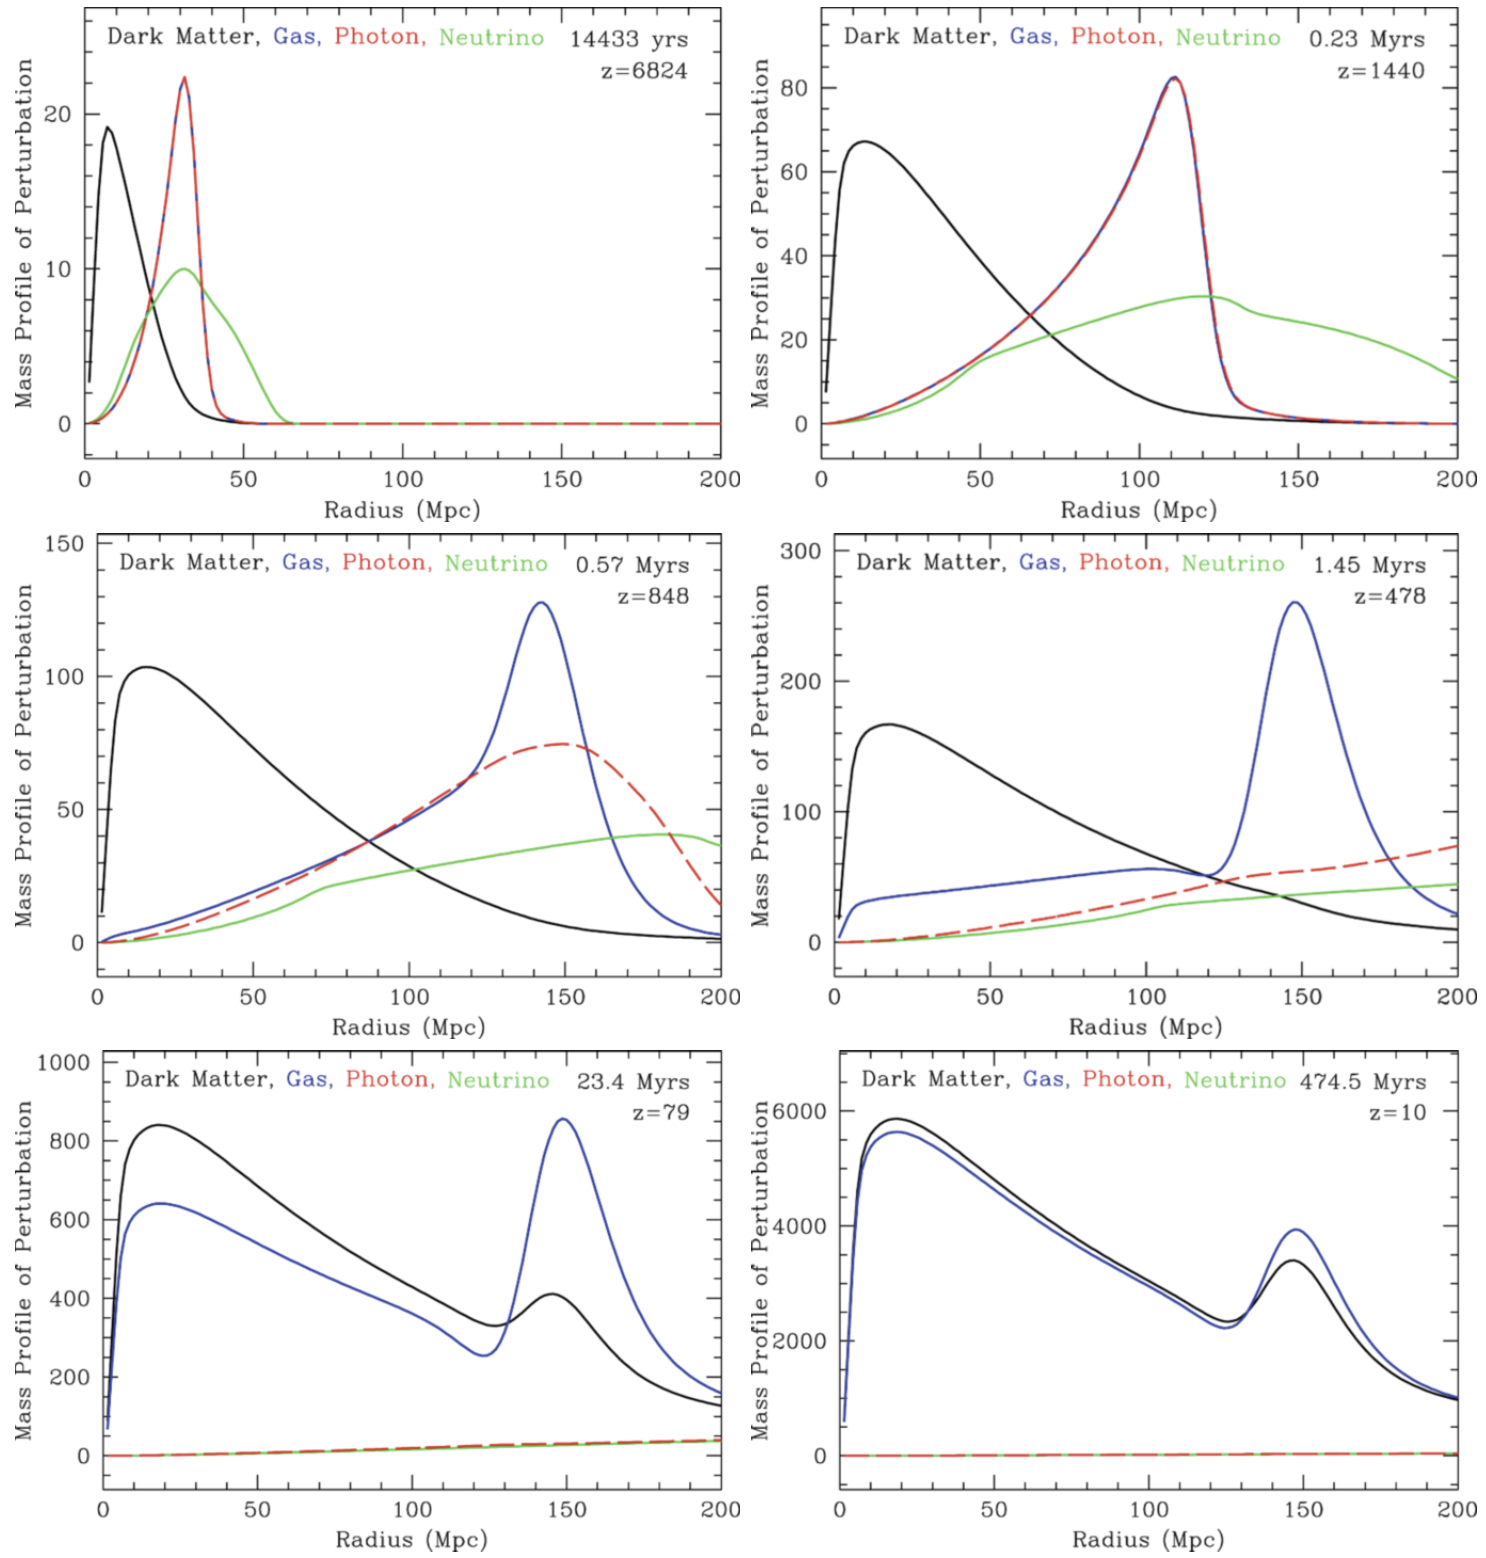
\includegraphics[width=15cm]{figures/cosmology/PerturbationEvolution.png}
    \centering
    \caption{\footnotesize{Evolution in time of an initial density peak in all components of the cosmic matter. \textit{Top left}: Near the initial time, the photons and baryons travel outward as a pulse. \textit{Top right}: Approaching recombination, one can see the wake in the cold dark matter raised by the outward-going pulse of baryons and relativistic species. \textit{Middle left}: At recombination, the photons leak away from the baryonic perturbation. \textit{Middle right}: With recombination complete, we are left with a CDM perturbation toward the center and a baryonic perturbation in a shell. \textit{Bottom left}: Gravitational instability now takes over, and new baryons and dark matter are attracted to the overdensities. \textit{Bottom right}: At late times, the baryonic fraction of the perturbation is near the cosmic value, because all of the new material was at the cosmic mean. Source: D.J. Eisenstein et al. 2007, On the Robustness of the Acoustic Scale in the Low-Redshift Clustering of Matter, ApJ 664, 660, p. 662, Fig. 1. Figure taken from Schneider (2006).}}
    \label{fig:perturbationevolution}
\end{figure}

{\noindent}There are some other interesting aspects of the physics of this epoch that are worth mentioning. First is that the outgoing wave does not actually stop at $z\sim10^3$ but instead slows around $z\sim500$. This is partially due to the fact that decoupling is not coincident with recombination but is also because the coupling to the growing mode is actually dominated by the velocity field, rather than the density field, at $z\sim10^3$. In other words, the compressing velocity field in front of the wave actually keys the instability at a later time.

{\noindent}Two other aspects that may be surprising at first
glance are that the outgoing pulse of neutrino overdensity does not actually remain as a delta function, as one might expect for a population traveling radially outward at the speed of light, and that the CDM perturbation does not remain at the origin, as one would expect for a cold species. Both of these effects are due to a hidden assumption in the initial conditions: although the density field is homogeneous everywhere but the origin, the velocity field cannot be for a growing mode. To keep the bulk of the universe homogeneous while growing a perturbation at the origin, matter
must be accelerating toward the center; this acceleration is supplied by the gravitational force from the central overdensity. However, in the radiation-dominated epoch the outward-going pulse of neutrinos and photons is carrying away most of the energy density of the central perturbation. This outward-going pulse decreases the acceleration, causing the inward flow of the homogeneous bulk to deviate from the divergenceless flow and generating the behavior of the CDM and neutrinos mentioned above. Essentially,
the outgoing shells of neutrinos and photons raise a wake in the homogeneous distribution of CDM away from the origin
of the perturbation.

{\noindent}The smoothing of the CDM overdensity from a delta function at the origin is the famous small-scale damping of the CDM power spectrum in the radiation-dominated epoch. The overdensity raised decreases as a function of radius because the radiation is decreasing in energy density relative to the inertia of the CDM; in the matter-dominated regime, the outward-going radiation has no further effect. A universe with more radiation causes a larger effect that extends to larger radii; this corresponds to the shift in the CDM power spectrum with the matter-to-radiation ratio.

{\noindent}Returning to the major conceptual point, that of the shell of overdensity left at the sound horizon, we see immediately that the sound horizon provides a standard ruler. The radius of the shell depends simply on the sound speed and the amount of propagation time. The sound speed is set by the balance of radiation pressure and inertia from the baryons; this is controlled simply by the baryon-to-photon ratio, which is $\Omega_bh^2$. The propagation time depends on the expansion rate in the matter-dominated and radiation-dominated regimes; this in turn depends on the redshift of matter-radiation equality, which depends only on $\Omega_mh^2$ for the standard assumption of the radiation density (i.e., the standard cosmic neutrino and photon backgrounds and nothing else).

{\noindent}The sound waves in the baryon-photon fluid, the baryonic acoustic oscillations (BAOs), are observable today. Since at recombination, the photons interacted with matter for the last time, the CMB radiation provides us with a picture of the density fluctuations at the epoch of recombination. Our observable cosmic microwave sky essentially is a picture of a two-dimensional cut at fixed time (the time of last scattering) through the density field of the baryons. A cut through an ensemble of sound waves shows an instantaneous picture of these waves. Hence, they are expected to be visible in the temperature distribution of the CMB. This is indeed the case: these BAOs imprint one of the most characteristic features on the CMB anisotropies. Since the sound waves are damped once they are inside the sound horizon, the largest amplitude waves are those whose wavelength equals the sound horizon at recombination.

{\noindent}We have argued that the baryons, once they are no longer coupled to radiation and thus become pressureless, fall into the potential wells of the dark matter. This happens because the dark matter fluctuations can grow while the baryonic fluctuations could not due to the photon pressure, and because the mean density of dark matter is substantially larger than that of the baryons. This is almost the full story, but not entirely: baryons make about 15\% of the total matter density, and are therefore not negligible. After recombination, the BAOs are frozen, like standing waves, and thus the total matter fluctuations are a superposition of the dark matter inhomogeneities and these standing waves. Whereas the dark matter dominates the density fluctuations, a small fraction of the matter also follows the inhomogeneities created by the standing waves. Since these waves have a characteristic length scale (the sound horizon at recombination) this characteristic length scale should be visible in the properties of the matter distribution even today. The correlation function of galaxies contains a characteristic feature at the length scale $r_s$. Hence, relics of the sound waves in the pre-recombination era are even visible in the current Universe. The effects of the BAOs are included in the transfer function $T(k)$, which thus shows some low-amplitude oscillations, often called `wiggles'.

{\noindent}The distance that acoustic waves can propagate in the first million years of the Universe is measurable not only in the cosmic microwave background (CMB) anisotropies but also in the late-time clustering of galaxies.

\subsubsection{Follow-up Questions}

\begin{itemize}
    \item How do we observe the power spectrum?
    \item What is its relation to BAOs and the $C_\ell$ power spectrum?
    \item Do we see super-horizon modes (modes larger than the universe's event horizon) in the evolved matter power spectrum?
    \item What actually causes the damping during the radiation-dominated era?
    \item Why do modes outside the horizon grow?
\end{itemize}

% --------------------------------------------------------------
%
%                           4. 
%
% --------------------------------------------------------------

\newpage
\subsection{Question 4}

State and explain three key pieces of evidence for a Big Bang origin for the observable Universe.

\subsubsection{Short answer}

The success of the Big Bang (BB) rests on three observational pillars:

\begin{enumerate}
    \item Hubble's Law exhibiting expansion: The first key observation to the modern era of cosmology that the Universe is expanding. If the Universe is expanding at the present time, then by `turning back the clock' the Universe must have been much smaller in the past. Hence, the BB.
    \item Light element abundances which are in accord with Big Bang nucleosynthesis: When the Universe was still a very hot plasma, the extreme radiation field ensured that any nucleus produced would be immediately photoionized by a high energy photon. As the Universe cooled (via expansion) well below the typical binding energies of nuclei, light elements began to form. Knowing the conditions of the early Universe and the relevant cross sections, one can calculate the expected primordial abundances of these light elements. Such predictions are consistent with measurements.
    \item The blackbody radiation left over from the first few hundred thousand years, the cosmic microwave background: The fact that the early Universe was very hot and dense meant that the baryonic matter was well coupled with the radiation field implying thermal equilibrium (TE) of photons. In TE, photons should follow the blackbody (or Planck) function in which the energy density is only dependent on temperature. As it turns out, the CMB radiation is the most accurate BB curve yet to be measured!
\end{enumerate}

\subsubsection{Additional context}

1. \textbf{Hubble's Law}

{\noindent}We have good evidence that the Universe is expanding. This means that early in its history, the distances between galaxies was smaller than it is today. It's convenient to describe this expansion effect by introducing the \textbf{scale factor} $a$, whose present value is equal to one ($a(t_0)\equiv1$). At earlier times, $a$ was much smaller than it is today -- hence, the Big Bang. 

{\noindent}The first key observation to the modern era of cosmology was the discovery of an expanding Universe. This is popularly credited to Edwin Hubble in 1929, but in fact the honour lies with Vesto Slipher more than 10 years earlier. Slipher was measuring spectra of nebulae whose nature was still under hot debate at that time. Observations of Hubble settled this debate in 1924 when he discovered \textit{Cepheid variables} in M31 (Andromeda) establishing a distance of roughly $1\,{\rm Mpc}$. More than a decade earlier in 1913, Slipher had measured the spectrum of M31 and found that it was approaching Earth at a velocity of over $200\,{\rm km\,s^{-1}}$. Over the next decade, he measured Doppler shifts for dozens of galaxies: with only a few exceptions, they were redshifted. By the time Hubble arrived, the basics of relativistic cosmology were already worked out and predictions existed that galaxy redshifts should increase with distance. It's hard to know how much these influenced Hubble, but by 1929 he had obtained Cepheid distances towards 24 galaxies along with their redshifts and claimed that they followed the empirical linear relationship:

\begin{align*}
    v = H_0 d ~ [{\rm km\,s^{-1}}],
\end{align*}

{\noindent}citing theoretical predictions as a possible explanation. At the time, Hubble estimated $H_0 \approx 500\,{\rm km\,s^{-1}\,Mpc^{-1}}$ because his calibration of Cepheid variables was in error. The best modern value is currently $H_0 = 70\,{\rm km\,s^{-1}\,Mpc^{-1}}$.

\begin{figure}[h]
    \floatbox[{\capbeside\thisfloatsetup{capbesideposition={right,center},capbesidewidth=4cm}}]{figure}[\FBwidth]
    {\caption{\footnotesize{The original Hubble diagram (Hubble, 1929). Velocities of distant galaxies (units should be ${\rm km\,s^{-1}}$) are plotted vs distance (units should be ${\rm Mpc}$). Solid (dashed) line is the best fit to the filled (open) points which are corrected (uncorrected) for the Sun's motion. Image taken from Dodelson (2003).}}
    \label{fig:hubblediagram}}
    {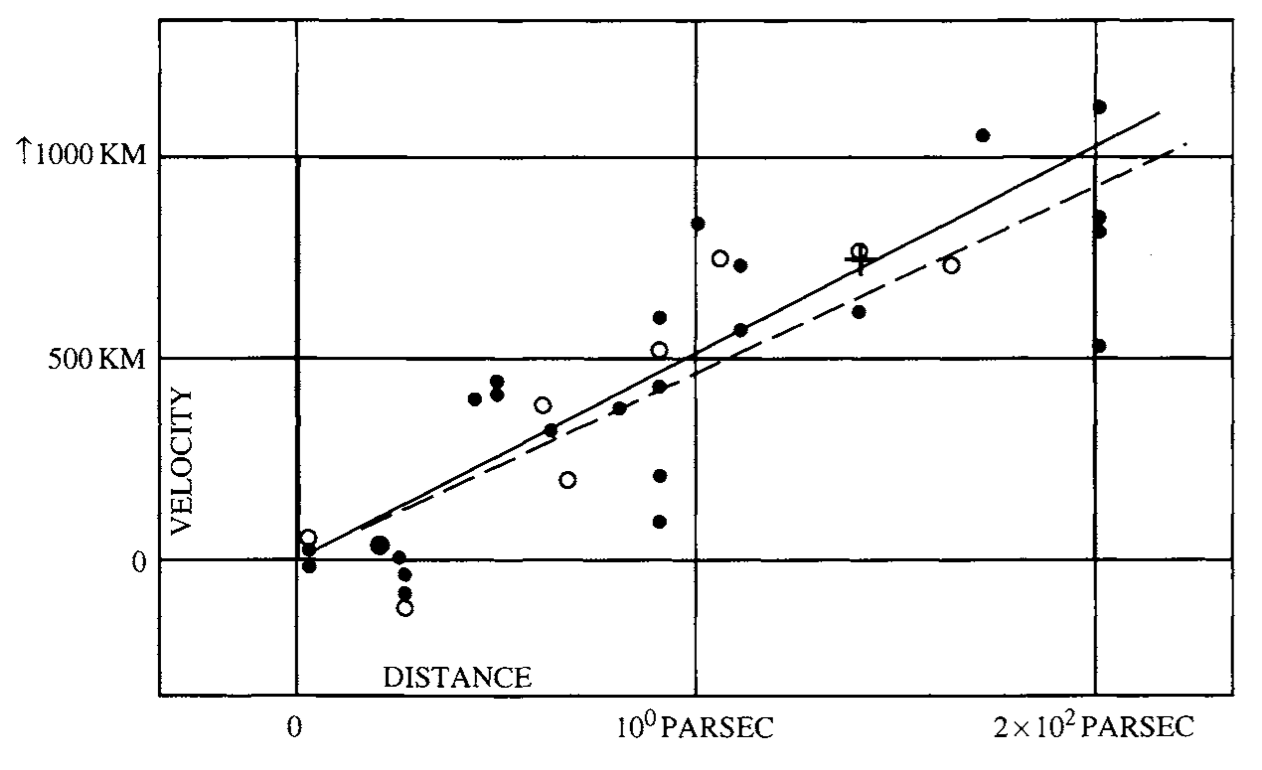
\includegraphics[width=10cm]{figures/cosmology/HubbleDiagram.png}}
\end{figure}

{\noindent}Recall that the wavelength of light or sound emitted from a receding object is stretched out (i.e., Doppler shifted) so that the observed wavelength is larger than the emitted one. It is convenient to define this stretching factor as the redshift $z$:

\begin{align*}
    1+z \equiv \frac{\lambda_0}{\lambda} = \frac{1}{a} ~ [{\rm dimensionless}],
\end{align*}

{\noindent}or

\begin{align*}
    (1+z)^{-1} \equiv \frac{\lambda}{\lambda_0} = a ~ [{\rm dimensionless}].
\end{align*}

{\noindent}For low redshifts, the standard Doppler formula applies and $z \sim v/c$. Therefore, a measurement of the amount by which absorption and/or emission lines are redshifted is a direct measure of how fast the structures in which they reside are receding from us. Hubble's diagram is shown in Figure \ref{fig:hubblediagram}, which shows not only that distant galaxies appear to be receding from us, but that the trend increases linearly with distance which is exactly what we would expect for an expanding Universe.

{\noindent}The Hubble diagram is still the most direct evidence we have that the universe is expanding. Current incarnations use the same principle as the original: find the distance and the redshift of distant objects. Measuring redshifts is straightforward; the hard part is determining distances for objects of unknown intrinsic brightness. One of the most popular techniques is to try to find a standard candle, a class of objects which have the same intrinsic brightness. Any difference between the apparent brightness of two such objects then is a result of their different distances from us. This method is typically generalized to find a correlation between an observable and intrinsic brightness. For example, \textbf{Cepheid variables} are stars for which intrinsic brightness is tightly related to their pulsation period.

\begin{figure}[h]
    \floatbox[{\capbeside\thisfloatsetup{capbesideposition={right,center},capbesidewidth=4cm}}]{figure}[\FBwidth]
    {\caption{\footnotesize{Hubble diagram from distant Type la supernovae. Top panel shows apparent magnitude (an indicator of the distance) vs redshift. Lines show the predictions for different energy contents in the universe, with $\Omega_M$ the ratio of energy density today in matter compared to the critical density and $\Omega_\Lambda$ the ratio of energy density in a cosmological constant to the critical density. Bottom panel plots the residuals, making it clear that the high-redshift supernovae favor a $\Lambda$-dominated universe over a matter-dominated one. Figure taken from Dodelson (2003).}}
    \label{fig:hubblediagram_modern}}
    {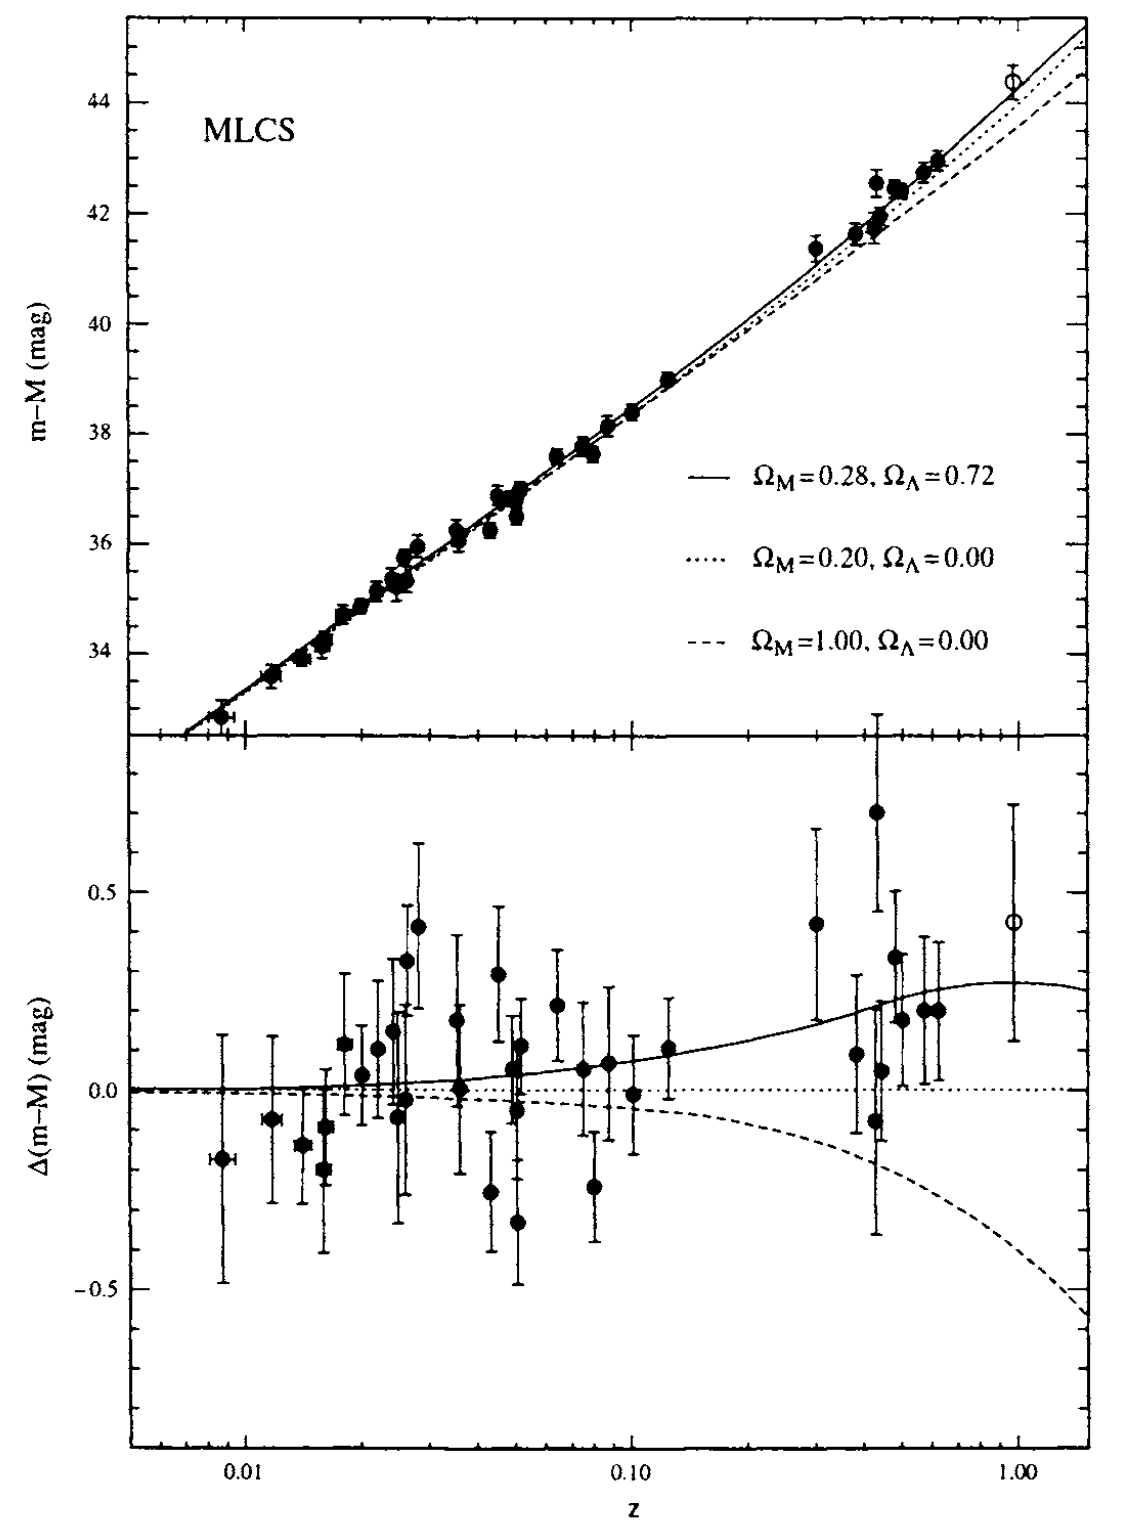
\includegraphics[width=11cm]{figures/cosmology/HubbleDiagram_modern.png}}
\end{figure}

{\noindent}As seen in Figure \ref{fig:hubblediagram_modern}, the standard candle that can be seen at largest distances is a Type la supernova. Since they are so bright, supernovae can be used to extend the Hubble diagram out to very large redshifts (the current record is of order $z\sim1.7$), a regime where the simple Doppler law ceases to work. Figure \ref{fig:hubblediagram_modern} shows a recent Hubble diagram using these very distant objects. The three curves in Figure \ref{fig:hubblediagram_modern} depict three different possibilities: flat matter dominated; open; and flat with a cosmological constant ($\Omega$). The high-redshift data are now good enough to distinguish among these possibilities, strongly disfavoring the previously favored flat, matter-dominated universe. The current best fit is a universe with about 70\% of the energy in the form of a cosmological constant, or some other form of dark energy.

{\noindent}2. \textbf{Big Bang Nucleosynthesis}

{\noindent}When the universe was much hotter and denser, when the temperature was of order an ${\rm MeV/k_B}$, there were no neutral atoms or even bound nuclei. The vast amounts of radiation in such a hot environment ensured that any atom or nucleus produced would be immediately destroyed by a high energy photon. As the universe cooled well below the binding energies of typical nuclei, light elements began to form. Knowing the conditions of the early universe and the relevant nuclear cross-sections, we can calculate the expected primordial abundances of all the elements.

\begin{figure}[h]
    \floatbox[{\capbeside\thisfloatsetup{capbesideposition={left,center},capbesidewidth=4cm}}]{figure}[\FBwidth]
    {\caption{\footnotesize{BBN predictions of the primordial abundances of light elements as a function of today’s baryon density ($\rho_{b,0}$ lower axis) and the corresponding density parameter $\Omega_b$ where $h=0.65$ was assumed. The vertical extent of the rectangles marks the measured values of the abundances (top: He$^4$, center: D, bottom: Li$^7$). The horizontal extent results from the overlap of these intervals with curves computed from theoretical models. The ranges in $\Omega_b$ that are allowed by these three species do overlap, as is indicated by the vertical strip. The deuterium measurements yield the most stringent constraints for $\Omega_b$. Figure taken from Schneider (2006).}}
    \label{fig:bbn_prediction}}
    {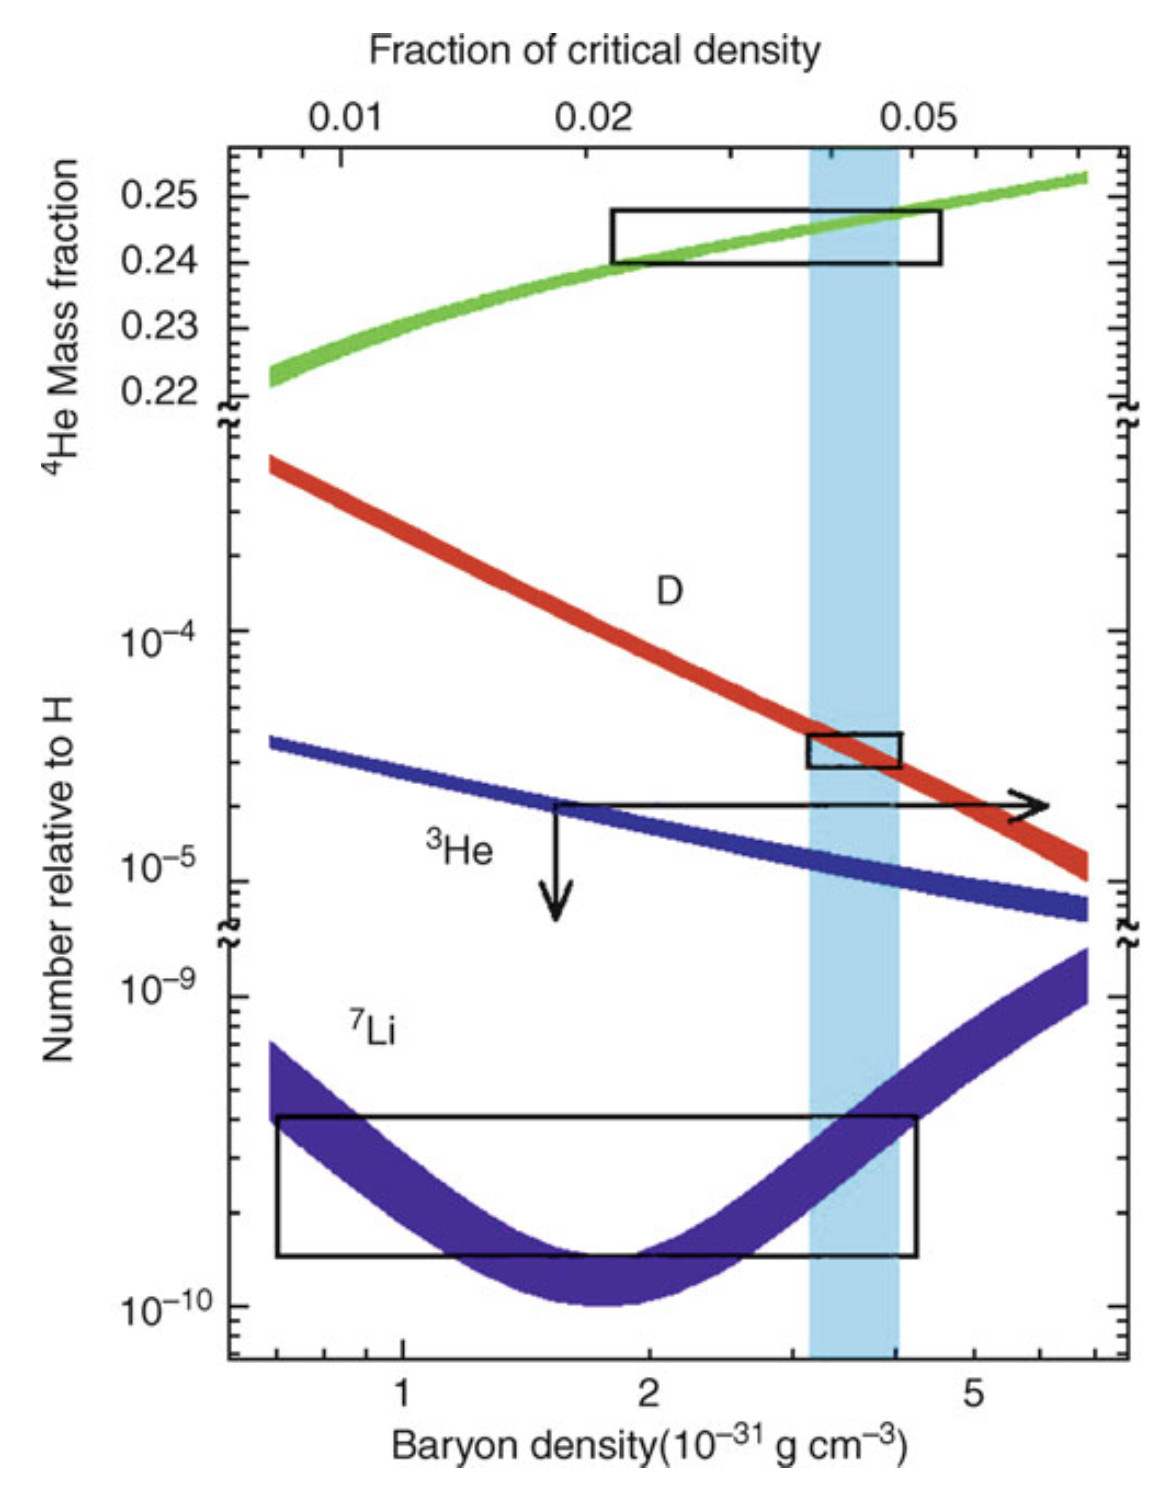
\includegraphics[width=10cm]{figures/cosmology/BBN_prediction.png}}
\end{figure}

{\noindent}Figure \ref{fig:bbn_prediction} shows the predictions of Big Bang Nucleosynthesis (BBN) for the light element abundances\footnote{Recall nuclear notation: The 4 in $^4$He refers to the total number of nucleons (protons and neutrons). So $^4$He has two neutrons and two protons, while $^3$He has two protons and one neutron.}. The boxes and arrows show the current estimates for the light element abundances. These are consistent with the predictions, and this consistency test provides yet another ringing confirmation of the Big Bang. The theoretical predictions depend on the density of protons and neutrons at the time of nucleosynthesis. The combined proton plus neutron density is called the \textbf{baryon density} ($\rho_b$) since both protons and neutrons have baryon number one and these are the only baryons around at the time. Thus, BBN gives us a way of measuring the baryon density in the universe. Since we know how those densities scale as the universe evolves (they fall as $a^{-3}$), we can turn the measurements of light element abundances into measures of the baryon density today.

{\noindent}In particular, the measurement of primordial deuterium pins down the baryon density extremely accurately to only a few percent of the critical density. Ordinary matter (baryons) contributes at most 5\% of the critical density (i.e., $\Omega_b = 0.005$). Since the total matter density today is almost certainly larger than this -- direct estimates give values of order 20-30\% — nucleosynthesis provides a compelling argument for non-baryonic dark matter.

\begin{figure}[h]
    \floatbox[{\capbeside\thisfloatsetup{capbesideposition={left,center},capbesidewidth=4cm}}]{figure}[\FBwidth]
    {\caption{\footnotesize{Spectrum from a distant QSO (Buries, Nollett, and Turner, 1999). Absorption of photons with rest wavelength $1216$ {\AA} corresponding to the (n = 1) to (n = 2) state of hydrogen is redshifted up to $1216(1+3.572)$ \AA. Bottom panel provides details of the spectrum in this range, with the the presence of deuterium clearly evident. Figure taken from Dodelson (2003).}}
    \label{fig:deuterium}}
    {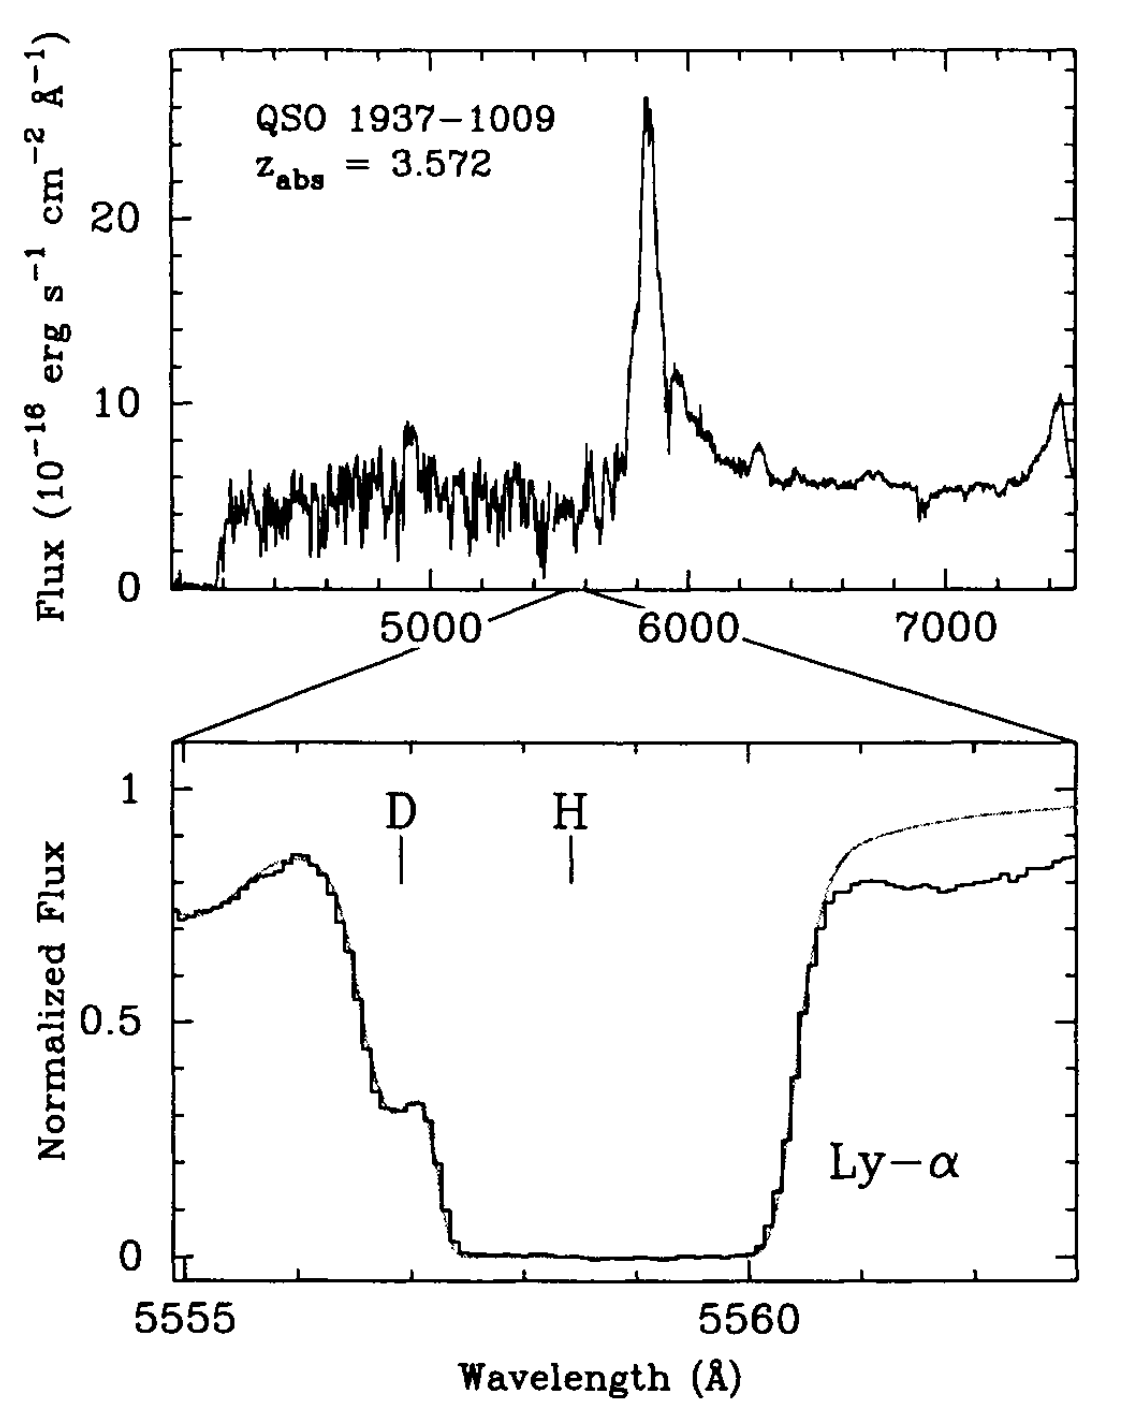
\includegraphics[width=10cm]{figures/cosmology/deuterium.png}}
\end{figure}

{\noindent}The deuterium measurements (Buries \& Tytler, 1998) are the new developments in the field. These measurements are so exciting because they explore the deuterium abundance at redshifts of order 3-4, well before much processing could have altered the primordial abundances. Figure \ref{fig:deuterium} shows one such detection. The basic idea is that light from distant QSOs is absorbed by intervening neutral hydrogen systems. The key absorption feature arises from transition from the ground state (n=1) of hydrogen to the first excited state (n = 2), requiring a photon with wavelength $\lambda = 1215.7$ \AA. Since photons are absorbed when exciting hydrogen in this fashion, there is a trough in the spectrum at {\AA}, redshifted by a factor of $(1+z)$. The corresponding line from deuterium should be (i) shifted over by $0.33(1+z)$ {\AA} and (ii) much less damped since there is much less deuterium. Figure \ref{fig:deuterium} shows just such a system; there are now half a dozen with detections precisely in the neighborhood shown in Figure \ref{fig:bbn_prediction}. Note that the steep decline in deuterium as a function of baryon density helps here: even relatively large errors in deuterium measurements translate into small errors on the baryon density.

{\noindent}3. \textbf{Cosmic Microwave Background (CMB)}

{\noindent}The CMB offers us a look at the universe when it was only $\sim 380,000$ years old. The photons in the CMB last scattered off electrons at $z \sim 1100$; since then they have traveled freely through space. When we observe them today, they literally come from the earliest moments of time. They are therefore the most powerful probes of the early Universe. If an object is opaque then the protons, neutrons, electrons, and photons which it contains frequently interact and attain \textit{thermal equilibrium}. A crucial fact about the CMB is that the collisions between electrons and photons before last scattering ensured that the photons were in equilibrium. That is, they should have a blackbody spectrum. When a system is in thermal equilibrium, the density of photons in the system as a function of photon energy depends only on the system temperature $T$. It doesn't matter whether the system is a tungsten filament or a sphere of ionized hydrogen and helium.

\begin{figure}[h]
    \floatbox[{\capbeside\thisfloatsetup{capbesideposition={right,center},capbesidewidth=4cm}}]{figure}[\FBwidth]
    {\caption{\footnotesize{Intensity of cosmic microwave radiation as a function of wavenumber from Far InfraRed Absolute Spectrophotometer (FIRAS) (Mather et al., 1994), an instrument on the COBE satellite. Hidden in the theoretical blackbody curve are dozens of measured points, all of which have uncertainties smaller than the thickness of the curve! Figure taken from Dodelson (2003).}}
    \label{fig:cmb_cobe}}
    {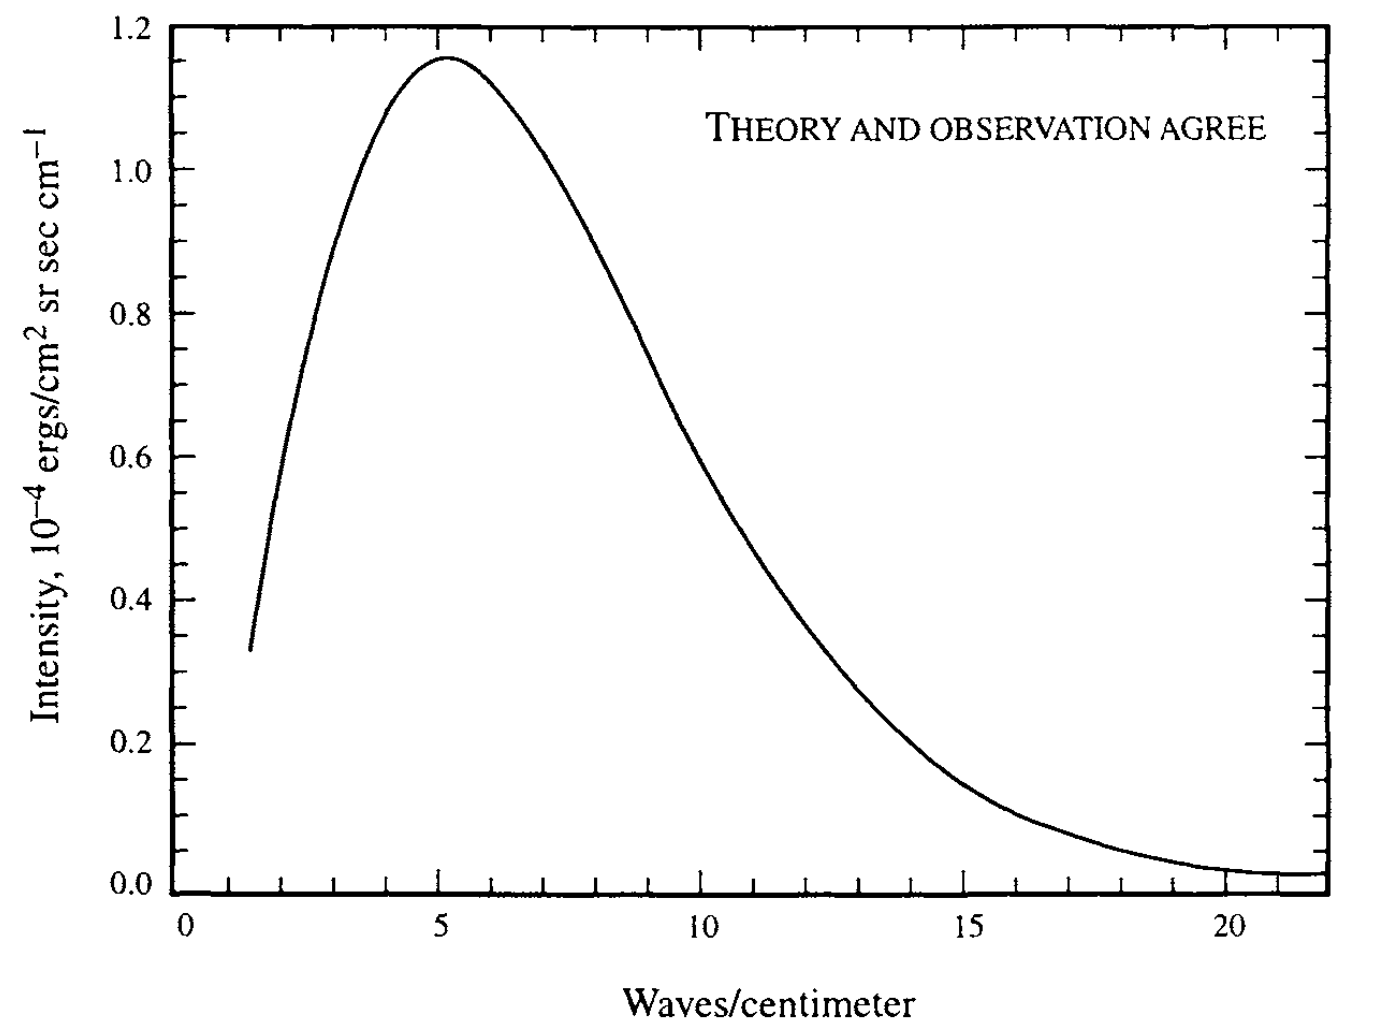
\includegraphics[width=10cm]{figures/cosmology/CMB_COBE.png}}
\end{figure}

{\noindent}The specific intensity of a gas of photons following a blackbody spectrum is called the \textbf{Planck function}:

\begin{align*}
    I_\nu = B_\nu(T) = \frac{2h\nu^3}{c^2} \frac{1}{\exp({h\nu/k_BT}) - 1} ~ [{\rm erg\,s^{-1}\,cm^{-2}\,Hz^{-1}\,sr^{-1}}].
\end{align*}

{\noindent}Figure \ref{fig:cmb_cobe} shows the remarkable agreement between this prediction of Big Bang cosmology and the observations by the FIRAS instrument aboard the COBE spacecraft. We have been told that detection of the $3\,{\rm K}$ background by Penzias and Wilson in the mid-1960s was sufficient evidence to decide the controversy in favor of the Big Bang over the Steady State universe. Penzias and Wilson, though, measured the radiation at just one wavelength. If even their one-wavelength result was enough to tip the scales, the current data depicted in Figure \ref{fig:cmb_cobe} should send skeptics from the pages of physics journals to the far reaches of radical Internet chat groups.

{\noindent}The photons which make up the cosmic microwave background (CMB) today have a well-measured temperature $T_\mathrm{CMB} = 2.725 \pm 0.002\,{\rm K}$. A photon with an energy $k_BT_\mathrm{CMB}$ today has a wavelength $hc/k_BT_\mathrm{CMB}$. Early on, when the scale factor was smaller than it is today, this wavelength would have been correspondingly smaller. Since the energy of a photon is inversely proportional to its wavelength, the photon energy would have been larger than today by a factor of $1/a$. This argument applied to the thermal bath of photons implies that the temperature of the plasma as a function of time is

\begin{align*}
    T(t) = \frac{T_0}{a(t)} ~ [{\rm K}].
\end{align*}

{\noindent}At early times, then, the temperature was higher than it is today.

{\noindent}The energy density of each component of the Universe is equal to the number density of each corresponding component times its average energy. The primary energy density components of the Universe includes radiation, matter (baryons and dark matter), and dark energy. Since photon energy scales as $a^{-1}$ in addition to the number density which scales as $a^{-3}$, the energy density of radiation should scale as $a^{-4}$. The energy density of non-relativistic particles, such as baryons, have a constant rest mass energy. Since their number density scales inversely proportional to volume, the energy density of matter scales as $a^{-3}$. Dark energy (introduced as a cosmological constant) is believed to have a constant energy density. While matter, and possibly a cosmological constant, dominate the current cosmological landscape, radiation must have been the dominant constituent of the Universe due to its energy density scaling of $a^{-4}$. Figure \ref{fig:energydensityscaling} illustrates how radiation, matter, and the cosmological constant energy density components evolve with time.

\begin{figure}[h]
    \floatbox[{\capbeside\thisfloatsetup{capbesideposition={right,top},capbesidewidth=4cm}}]{figure}[\FBwidth]
    {\caption{\footnotesize{Energy density vs scale factor for different constituents of a flat Universe. Shown are non-relativistic matter, radiation, and a cosmological constant. All are in units of the critical density today. Even though matter and cosmological constant dominate today, at early times, the radiation density was largest. The epoch at which matter and radiation are equal is $a_\mathrm{eq}$. Image taken from Dodelson (2003).}}
    \label{fig:energydensityscaling}}
    {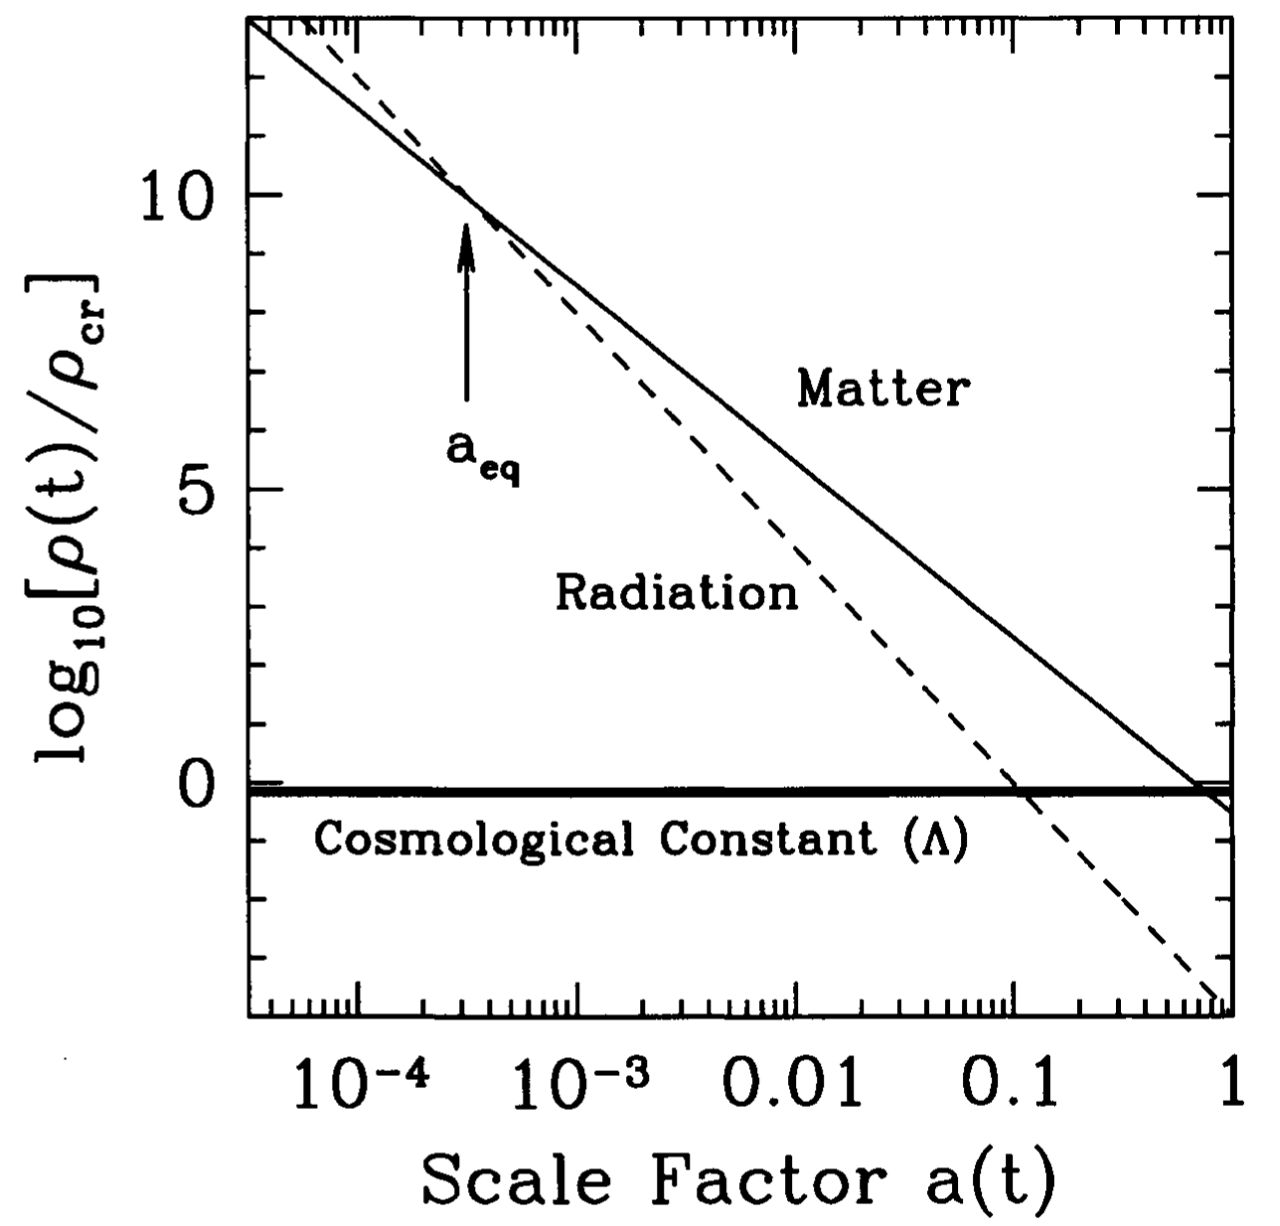
\includegraphics[width=10cm]{figures/cosmology/EnergyDensityScaling.png}}
\end{figure}

{\noindent}The CMB was detected by Arno Penzias \& Robert Wilson in 1965 and were awarded the 1978 Nobel prize in physics; they accomplished this by locating an unaccounted-for source of noise in a radio telescope at Bell Laboratories being used to study our own Galaxy. This excess ``noise'' was isotropic and constant with time, so it couldn't be associated with an isolated celestial source. Wilson and Penzias were puzzled until they were put into touch with Robert Dicke and his research group at Princeton University. Dicke had deduced that the Universe, if it started in a hot dense state, should now be filled with microwave radiation. The timing of the discovery was especially ironic, given that instruments were underway at that time to test the theoretical prediction that such a background should exist.

{\noindent}When the Universe was fully ionized, photons interacted primarily with electrons via Thomson scattering (the low energy limit of Compton scattering): 

\begin{align*}
    \gamma + e^{-} \rightarrow \gamma + e^{-}.
\end{align*}

{\noindent}Thomson scattering is an elastic process whereby energy and momentum are transferred between the photon and electron. The cross-section for Thomson scattering is the Thomson cross-section of 

\begin{align*}
    \sigma_e = 6.65 \times 10^{-29} ~ [{\rm m^2}].
\end{align*}

{\noindent}The mean free path of a photon -- that is, the mean distance it travels before scattering from an electron-- is therefore

\begin{align*}
    \ell_\mathrm{mfp} = \frac{1}{n_e\sigma_e} ~ [{\rm m}].
\end{align*}

{\noindent}When the baryonic component of the universe is fully ionized, $n_e = n_p = n_b$. Currently, the number density of baryons is $n_{b,0} = 0.22\,{\rm m^{-3}}$. The number density of conserved particles, such as baryons, goes with the scale factor as $1/a^3$, so when the early universe was fully ionized, the free electron density was

\begin{align*}
    n_e = n_b = \frac{n_{b,0}}{a^3} ~ [{\rm m^{-3}}].
\end{align*}

{\noindent}Since photons travel with speed $c$, the rate at which a photon undergoes scattering interactions is

\begin{align*}
    \Gamma = \frac{c}{\ell_\mathrm{mfp}} = n_e\sigma_ec ~ [{\rm s^{-1}}].
\end{align*}

{\noindent}Using the fact that $n_e = n_b = n_{b,0}/a^3$ for a fully-ionized Universe,

\begin{align*}
    \Gamma = \frac{n_{b,0}\sigma_ec}{a^3} = \frac{4.4\times10^{-21}}{a^3} ~ [{\rm s^{-1}}].
\end{align*}

{\noindent}The photons remain coupled to the electrons as long as their scattering rate, $\Gamma$, is larger than $H$, the rate at which the Universe expands; this is equivalent to saying that their mean free path $\ell_\mathrm{mfp}$ is shorter than the Hubble distance $c/H$.

{\noindent}Measuring the spectrum of the CMB, and confirming that it is indeed a blackbody, is not a simple task, even with modern technology. The current energy per CMB photon, $\sim 6 \times 10^{−4}\,{\rm eV}$, is tiny compared to the energy required to break up an atomic nucleus ($\sim 1\,{\rm MeV}$) or even the energy required to ionize an atom ($\sim 10\,{\rm eV}$). However, the mean photon energy is comparable to the energy of vibration or rotation for a small molecule such as H$_2$O. Thus, CMB photons can zip along for more than 13 billion years through the tenuous intergalactic medium, then be absorbed a microsecond away from the Earth’s surface by a water molecule in the atmosphere. Microwaves with wavelengths shorter than λ ∼ 3 cm are strongly absorbed by water molecules.

{\noindent}The CMB can be measured at wavelengths shorter than 3 cm by observing from high-altitude balloons or from the South Pole, where the combination of cold temperatures and high altitude keeps the atmospheric humidity low. The best way to measure the spectrum of the CMB, however, is to go completely above the damp atmosphere of the Earth. The CMB spectrum was first measured accurately over a wide range of wavelengths by the COsmic Background Explorer (COBE) satellite, launched in 1989, into an orbit 900 km above the Earth’s surface. COBE actually contained three different instruments. The Diffuse InfraRed Background Experiment (DIRBE) was designed to measure radiation at the wavelengths 0.001 mm < λ < 0.24 mm; at these wavelengths, it was primarily detecting stars and dust within our own Galaxy. The second instrument, called the Far InfraRed Absolute Spectrophotometer (FIRAS), was used to measure the spectrum of the CMB in the range $0.1\,{\rm mm} < \lambda < 10\,{\rm mm}$, a wavelength band which includes the peak in the CMB spectrum. The third instrument, called the Differential Microwave Radiometer (DMR), was designed to make full-sky maps of the CMB at three different wavelengths: $\lambda = 3.3\,{\rm mm}$, $5.7\,{\rm mm}$, and $9.6\,{\rm mm}$.

{\noindent}The most important fact we learned from our first 25 years of surveying the CMB was that the early Universe was very smooth. No anisotropies were detected in the early CMB. This period, while undoubtedly frustrating for observers searching for anisotropies, solidified the view of a smooth Big Bang. We are now moving on. We have discovered anisotropies in the CMB, indicating that the early Universe was not completely smooth. There were small perturbations in the cosmic plasma. To understand these, we must go beyond the Standard Model.


% --------------------------------------------------------------
%
%                           5. 
%
% --------------------------------------------------------------

\newpage
\subsection{Question 5}

Define and describe the ``tired light hypothesis" and the ``steady state universe'' as alternatives to the Big Bang. How have they been disproved observationally?

\subsubsection{Short answer}

{\noindent}\textbf{Tired Light Hypothesis:} The Tired Light Hypothesis states that the Universe is not expanding, but that photons simply lose energy as they move through space (by some unexplained means). Such a Universe would leads to a blurring of distant objects which is not observed.

{\noindent}\textbf{Steady State Theory:} The Steady State Theory states that matter is continuously being created as the Universe expands in such a way that the matter density remains constant, therefore discarding a beginning to the Universe and adhering to a perfect cosmological principle. The discovery of the Cosmic Microwave Background is commonly regarded as the observation which decisively tipped the scales in favor of the Big Bang model.

\subsubsection{Additional context}

{\noindent}\textbf{Tired Light Hypothesis:} The Tired Light Hypothesis states that the Universe is not expanding, but that photons simply lose energy as they move through space (by some unexplained means), with an exponential dependence on distance $r$ as

\begin{align*}
    E = E_0 \mathrm{e}^{(-r/R_0)} ~ [{\rm eV}],
\end{align*}

{\noindent}where $R_0$ is some constant. There is no known interaction that can degrade a photon's energy without also changing its momentum, which leads to a blurring of distant objects which is not observed.

{\noindent}\textbf{Steady State Theory:} The Steady State model was first proposed in the 1940's by Hermann Bondi, Thomas Gold, and Fred Hoyle, who were proponents of the \textit{perfect cosmological principle}, which states that not only are there no privileged locations in space, there are no privileged moments in time. Thus, a Steady State Universe is one in which the global properties of the universe, such as the mean density $\rho_0$ and the Hubble constant $H_0$, remain constant with time. It was proposed as an alternate theory to the Big Bang model of the Universe which states that matter is continuously being created as the Universe expands in such a way that the matter density remains constant, therefore discarding a beginning to the Universe and adhering to a perfect cosmological principle. Though the Steady State Theory is largely discredited today, its popularity in the 1940's pushed for supporting evidence of the Big Bang model. Interestingly, it was Fred Hoyle who coined the term `Big Bang' during a 1949 BBC interview: ``These theories were based on the hypothesis that all matter in the Universe was created in one big bang at a particular time in the remote past.''

{\noindent}In a Steady State Universe, the velocity-distance relation can be easily integrated:

\begin{align*}
    v &= H_0r ~ [{\rm km\,s^{-1}}]\\
    \frac{dr}{dt} &= H_0r \\
    \int \frac{dr}{r} &= \int H_0 dt \\
    \ln (r) &= H_0t \\
    r(t) &\propto e^{H_0t} [{\rm Mpc}].
\end{align*}

{\noindent}Note that $r \rightarrow 0$ only in the limit that $t \rightarrow -\infty$, so a Steady State Universe is infinitely old. If there existed an instant in time at which the universe started expanding (as in a Big Bang model), that would be a special moment, in violation of the assumed ``perfect cosmological principle''. 

{\noindent}The volume of a spherical region of space, in a Steady State model, increases exponentially with time:

\begin{align*}
    V(t) = \frac{4}{3}\pi r^3 \propto e^{H_0t} = e^{3H_0t} ~ [{\rm Mpc^3}].
\end{align*}

{\noindent}However, if the universe is in a steady state, the density of the sphere must remain constant. To have a constant density of matter within a growing volume, matter must be continuously created at a rate of

\begin{align*}
    \dot{M(t)}_{SS} = \rho_0 \dot{V(t)} = \rho_0 3 H_0 V(t) ~ [{\rm kg\,Gyr^{-1}}].
\end{align*}

{\noindent}If our own universe, with matter density $\rho_0 \sim 3 \times 10^{−27}\,{\rm kg\,m^{−3}}$, happened to be a Steady State universe, then matter would have to be created at a rate of 

\begin{align*}
    \frac{\dot{M(t)}_{SS}}{V(t)} = 3H_0\rho_0 \sim 6\times10^{-29} ~ [{\rm kg\,m^{-3}\,Gyr^{-1}}],
\end{align*}

{\noindent}which corresponds to creating roughly one hydrogen atom per cubic kilometer per year.

{\noindent}The Steady State model finally fell out of favor when observational evidence increasingly indicated that the perfect cosmological principle is not true; the properties of the universe \textit{do}, in fact, change with time. The discovery of the Cosmic Microwave Background is commonly regarded as the observation which decisively tipped the scales in favor of the Big Bang model.

% --------------------------------------------------------------
%
%                           6. 
%
% --------------------------------------------------------------

\newpage
\subsection{Question 6}

Why are only very light elements (H, D, He, and traces of Li) synthesized in the first three minutes of the Big Bang?

\subsubsection{Short answer}

Deuterium synthesis acted as the first bottleneck for nucleosynthesis of heavier elements. The deuteron (i.e., deuterium nucleus) has a binding energy of $2.225\,{\rm MeV}$ which is only $4.3$ times larger than $m_ec^2$ and $1.7$ times larger than the neutron-proton mass-energy difference. Therefore, typical photons are energetic enough to easily photoionize deuterium. The Universe must therefore cool to $T\sim10^9\,{\rm K}$, just below the binding energy of deuterium for the equilibrium to swing in favour of deuterium synthesis. This occurs at $t\sim3\,{\rm min}$. All the while, free neutrons are decaying with a half life of $t_n\sim15\,{\rm min}$. Since the simplest way to synthesize helium is by fusing deuterium, helium synthesis must await significant quantities of deuterium which happens at a temperature roughly one third that at which helium would be expected to dominate. Once significant nucleosynthesis begins, deuterium is rapidly converted into helium owing to its greater binding energy per nucleon ($7\,{\rm MeV}$ as opposed to $1.1\,{\rm MeV}$ for deuterium). This occurs at a temperature of roughly $0.1\,{\rm MeV}$, by which point the density and temperature of the Universe are too low for significant synthesis of heavier nuclei to proceed. 

\subsubsection{Additional context}

{\noindent}At sufficiently early times, the temperature of the Universe was that of the centre of the Sun ($1.55\times10^7\,{\rm K}$), where we know that nuclear reactions occur. Starting in the 1940's, Gamow considered the fascinating question of whether nuclear reactions were possible in the early Universe. He noted that the abundances of some elements in stars showed great regularities, especially a universal proportion of about 25\% helium by mass. This led to the vision that a chain of nuclear reactions in the early Universe could generate not only helium, but all elements. In 1957, the Burbidges, Fowler \& Hoyle showed that almost all elements could in fact be generated in stars, but the problem of helium remained. Gamow showed that its existence could be used to predict the present radiation temperature (as argued below).

{\noindent}It will be convenient to refer to particle masses and temperatures in nuclear physics units, which are ${\rm MeV}$. Some useful conversions are:

\begin{align*}
    1\,{\rm MeV} &= 10^{10.065}\,{\rm K} \\
    m_e &= 0.55\,{\rm MeV} \\
    m_p &= 939\,{\rm MeV} \\
    m_n-m_p &= 1.3\,{\rm MeV}.
\end{align*}

{\noindent}\textit{Neutron freezeout:}

{\noindent}After the annihilation between matter and anti-matter (below $\sim10^{13}\,{\rm K}$), the balance between neutrons and protons are maintained in equilibrium by weak interactions:

\begin{align*}
    p + e^-n \leftrightarrow n + \nu \\
    n + e^+ \leftrightarrow p + \bar{\nu}.
\end{align*}

{\noindent}While this persists, the relative number densities of neutrons and protons should vary according to a Boltzmann factor based on their rest energy difference of $1.3\,{\rm MeV}$:

\begin{align*}
    \frac{n_n}{n_p} = e^{-\Delta mc^2/k_BT} ~ [{\rm dimensionless}].
\end{align*}

{\noindent}The reason that neutrons exist today that the timescale for the weak interactions needed to keep this equilibrium set up eventually becomes longer than the expansion timescale. The reactions thus rapidly cease, and the proton-neutron ratio undergoes freezeout at some characteristic value which determined the He abundance. Since most He is $^4$He (i.e., two neutrons and two protons), the Helium mass fraction (denoted $Y$) is given by

\begin{align*}
    Y = \frac{4\times n_n/2}{n_n + n_p}  = \frac{2}{1 + n_n/n_n} ~ [{\rm dimensionless}]
\end{align*}

{\noindent}neglecting neutrons in other elements. So, $Y=0.25$ requires a neutron-proton freezeout $n_n/n_p\simeq1/7$. To calculate when the neutron-proton ratio undergoes freezeout, we need to know the rates of weak nuclear reactions. Fermi discovered how to calculate the relevant cross sections in the 1930s. Remember that, at $T\sim10^{10}~{\rm K}$, we are above the electron-proton energy threshold, so there exist thermal populations of both electrons and neutrinos to make the reaction $p+e^- \leftrightarrow n+\nu$ go equally well in either direction. All that is needed, therefore, is to consider either the reaction timescale for one proton immersed in a thermal bath of electrons or of one neutron immersed in a bath of neutrinos (the rates are the same). When this timescale equals the local Hubble time, $a(t)/\dot{a}(t)$, we get freezeout of the proton-neutron ratio. Taking the known weak interaction rates, this happens at

\begin{align*}
    T(n~{\rm freezeout}) \simeq 10^{10.14} {\rm K} \Rightarrow \frac{n_n}{n_p} \simeq 0.34.
\end{align*}

{\noindent}This number is not a precisely correct result because nucleosynthesis is a process that contains a number of interesting (but potentially confusing) coincidences:

\begin{enumerate}
  \item The freezeout condition was calculated assuming a temperature well above the electron mass threshold, but freezeout actually happens only a very little above this critical temperature.
  \item Neutrons are not stable: they decay spontaneously with the $e$-folding lifetime of $\tau_n=887\pm2\,{\rm s}$. Unless the frozen-out neutrons can be locked away in nuclei before $t=887\,{\rm s}$, the relic abundance will decay freely to zero. The freezeout point occurs at an age of a few seconds, so there are only a few $e$-foldings of expansion available in which to salvage some neutrinos.
\end{enumerate}

{\noindent}\textit{Locking up the neutrons:}

{\noindent}It may seem implausible that we can add one more coincidence -- i.e., that nuclear reactions will become important at about the same time -- this is just what happens. The Deuteron binding energy of $2.225\,{\rm MeV}$ is only $4.3$ times larger than $m_ec^2$ and only $1.7$ times larger than the neutron-proton mass difference. At higher temperatures, the strong interaction $n+p \leftrightarrow \mathrm{D}+\gamma$ is fast enough to produce deuterium, but thermal equilibrium favours a small deuterium fraction -- i.e., typical photons are energetic enough to disrupt deuterium nuclei very easily. The second key temperature in nucleosynthesis is therefore where the Universe has cooled sufficiently for the equilibrium to swing in favour of deuterium. In practice, this happens at a temperature a little below the deuteron binding energy. This is because the large photon to baryon ratio: even if photons lack sufficient energy to disintegrate deuterons, the rare ones in the tail of the distribution can still do the job. 

{\noindent}Nevertheless, the temperature at which deuterium switches from being rare to dominating the equilibrium is still at $k_BT$ of order the deuterium binding energy:

\begin{align*}
    T({\mathrm{Deuterium~formation}}) \simeq 10^{8.9}\,[{\rm K}],
\end{align*}

{\noindent}or at a time of about 3 minutes.

{\noindent}Notice that we have not needed to know the nuclear reaction rates that form deuterium, since the argument is an equilibrium one. However, if the matter density is too low, the nuclear reactions will freeze out before much deuterium has formed. Gamow took the known nuclear cross-sections and argued that the typical reaction time for deuterium formation had to be the cosmological age at that time (i.e., 3 minutes). This let him conclude that the matter density must have been about $10^{-3}\,{\rm kg\,m^{-3}}$ at that time. This gives a ratio of number densities of photons to nucleons, which is preserved as the Universe expands. Therefore, the present-day matter density allows a prediction of the present-day photon density, and hence its temperature. Alpher \& Herman used Gamow's argument to predict a current photon temperature of $4\,{\rm K}$ to $5\,{\rm K}$, which is impressively accurate. On the other hand, this prediction was based on a figure for the $z=0$ matter density that is probably too low by at least a factor of $100$, raising the temperature estimate by a factor of about 5. Actually, Gamow's argument is an inequality: there is a minimum matter density at $10^9\,{\rm K}$, but it could have been higher. The prediction for the current temperature is therefore really an upper limit. It works because the nuclear reactions are not too far from freeze out when deuterium forms.

{\noindent}The deuterium measurements (Buries and Tytler, 1998) are the new developments in the field. These measurements are so exciting because they explore the deuterium abundance at redshifts of order 3-4, well before much processing could have altered the primordial abundances. Figure \ref{fig:deuterium} shows one such detection. The basic idea is that light from distant QSOs is absorbed by intervening neutral hydrogen systems. The key absorption feature arises from transition from the ground state ($n=1$) of hydrogen to the first excited state ($n=2$), requiring a photon with wavelength $\lambda = 1215.7$ \AA. Since photons are absorbed when exciting hydrogen in this fashion, there is a trough in the spectrum at {\AA}, redshifted by a factor of $(1+z)$. The corresponding line from deuterium should be (i) shifted over by $0.33(1+z)$ {\AA} and (ii) much less damped since there is much less deuterium. Figure \ref{fig:deuterium} shows just such a system; there are now half a dozen with detections precisely in the neighborhood shown in Figure \ref{fig:bbn_prediction}. Note that the steep decline in deuterium as a function of baryon density helps here: even relatively large errors in deuterium measurements translate into small errors on the baryon density.

{\noindent}\textit{Formation of helium:}

{\noindent}The argument so far has produced a Universe consisting of just hydrogen and deuterium, but this is not realistic as one would expect $^4$He to be preferred on thermodynamic grounds, owing to its greater biding energy per nucleon ($7\,{\rm MeV}$ as opposed to $1.1\,{\rm MeV}$ for deuterium). In equilibrium, the first nuclei to come into existence in significant numbers should be $^4$He: the abundance of $^4$He relative to protons should reach unity at an energy of about $0.3\,{\rm MeV}$, at which point the relative abundance of deuterium is only $\sim10^{-12}$.

{\noindent}Since the simplest way to synthesize helium is by fusing deuterium, it is no surprise that the equilibrium prediction fails miserably in the expanding Universe: the production of helium must await the synthesis of significant quantities of deuterium which we have seen happens at a temperature roughly one third that at which helium would be expected to dominate. What the thermodynamic argument does show, however, is that it is expected that deuterium will be rapidly converted to helium once significant nucleosynthesis begins. This argument is what allows us to expect that the helium abundance can be calculated from the final $n_n/n_p$ ratio. The main reactions of importance are of course $2$-body ones, rather than the improbable coincidence of $2$ protons and $2$ neutrons all arriving at the same place simultaneously to make $^4$He in one go. The process starts by fusing deuterium to make either tritium and $^3$He, following which there are four main ways of reaching $^4$He (leaving aside rarer reactions involving residual free neutrons):

\begin{align*}
    \mathrm{D} + \mathrm{D} &\leftrightarrow \mathrm{^3He} + n \\
    \mathrm{D} + \mathrm{D} &\leftrightarrow \mathrm{T} + p \\ \\
    \mathrm{D} + \mathrm{D} &\leftrightarrow \mathrm{^4He} \\
    \mathrm{T} + p &\leftrightarrow \mathrm{^4He} \\
    \mathrm{D} + \mathrm{^3He} &\leftrightarrow \mathrm{^4He} + p \\
    \mathrm{D} + \mathrm{T} &\leftrightarrow \mathrm{^4He} + n.
\end{align*}

{\noindent}The same thermodynamic arguments that say helium should be favoured at temperatures around $0.1\,{\rm MeV}$ say that more massive nuclei would be preferred in equilibrium at lower temperatures still. A Universe that stayed in nuclear equilibrium as it cooled would eventually consist entirely of iron since this has the largest binding energy per nucleon. However, by the time helium synthesis is accomplished, the density and temperature are too low for significant synthesis of heavier nuclei to proceed. Apart from helium, the main nuclear residue of the Big Bang is therefore those deuterium nuclei that escape being mopped up into helium, plus a trace of $^3$He. The other intermediate produce, tritium, is not so strongly bound and and thus leaves no significant relic. There also exists extremely small fractions of other elements: $^7$Li ($\sim10^{-9}$ by mass) and $^7Be$ ($\sim10^{-11}$ by mass). The helium content in the Universe changes later by nuclear fusion in stars, which also forms heavier nuclei (`metals'). However, the total amount of helium produced in stars is expected to be smaller by about one order of magnitude compared to that in BBN.

{\noindent}In summary, nucleosynthesis starts at about $10^{10}\,{\rm K}$ when the Universe was about $1\,{\rm s}$ old, and effectively ends when it has cooled by a factor of 10, and is about 100 times older.

% --------------------------------------------------------------
%
%                           7. 
%
% --------------------------------------------------------------

\newpage
\subsection{Question 7}

Explain how and why Type Ia supernovae are used in the measurements of cosmological parameters.

\subsubsection{Short answer}

Type 1a are good standard candles -- they are very luminous and standardized. The average Type 1a has a peak luminosity of $L=4\times10^9\,\mathrm{L}_\odot$ which is 100,000 times brighter than even the brightest Cepheid variable. When $z\ll1$, the luminosity distance to the light source is

\begin{align*}
    d_L \approx \frac{c}{H_0}z \left(1+\frac{1-q_0}{2}z\right) ~ [{\rm Mpc}]
\end{align*}

{\noindent}The recipe for finding the Hubble constant and deceleration parameters is a simple one:

\begin{itemize}
    \item Measure the redshift $z$ and flux $F$ for each SN.
    \item Compute the luminosity distance $d_L=\sqrt{L/4\pi F}$ for each SN.
    \item Plot the recessional velocity $cz$ versus luminosity distance $d_L$.
    \item Measure the slope of the $cz$ versus $d_L$ relation when $z\ll1$; this gives $H_0$.
    \item At slightly larger values of $z$ (but still $<1$), the deviation of the plot from a straight line tells you the value of $q_0$.
\end{itemize}

\subsubsection{Additional context}

{\noindent}In recent years, the standard candle of choice among cosmologists has been Type Ia supernovae (SNe). A supernova may be loosely defined as an exploding star. Early in the history of supernova studies, when little was known about their underlying physics, supernovae were divided into two classes, on the basis of their spectra. Type I supernovae contain no hydrogen absorption lines in their spectra; Type II supernovae contain strong hydrogen absorption lines. Gradually, it was realized that all Type II supernovae are the same species of beast; they are massive stars ($M>8\,M_\odot$) whose cores collapse to form a black hole or neutron star when their nuclear fuel is exhausted. During the rapid collapse of the core, the outer layers of the star are thrown off into space. Type I supernovae are actually two separate species, which are called Type Ia and Type Ib. Type Ib supernovae, it is thought, are massive stars whose cores collapse after the hydrogen-rich outer layers of the star have been blown away in strong stellar winds. Thus, Type Ib and Type II supernovae are driven by very similar mechanisms -- their differences are superficial, in the most literal sense. Type Ia supernovae, however, are something completely different. They occur in close binary systems where one of the two stars in the system is a white dwarf; that is, a stellar remnant which is supported against gravity by electron degeneracy pressure. The transfer of mass from the companion star to the white dwarf eventually nudges the white dwarf over the Chandrasekhar limit of $1.4\,M_\odot$; this is the maximum mass at which the electron degeneracy pressure can support a white dwarf against its own self-gravity. When the Chandrasekhar limit is exceeded, the white dwarf starts to collapse until its increased density triggers a runaway nuclear fusion reaction. The entire white dwarf becomes a fusion bomb, blowing itself to smithereens; unlike Type II supernovae, Type Ia supernovae do not leave a condensed stellar remnant behind.

{\noindent}Within our Galaxy, Type Ia supernovae occur roughly once per century, on average. Although Type Ia supernovae are not frequent occurrences locally, they are extraordinarily luminous, and hence can be seen to large distances. The luminosity of an average Type Ia supernova, at peak brightness, is $L=4\times10^9\,\mathrm{L}_\odot$; that’s 100,000 times more luminous than even the brightest Cepheid. For a few days, a Type Ia supernova in a moderately bright galaxy can outshine all the other stars in the galaxy combined. Since moderately bright galaxies can be seen at $z\sim1$, this means that Type Ia supernovae can also be seen at $z\sim1$. Not only are Type Ia supernovae bright standard candles, they are also reasonably standardized standard candles. Consider Type Ia supernovae in the Virgo cluster. Although there’s only one Type Ia supernova per century in our own Galaxy, the total luminosity of the Virgo cluster is a few hundred times that of our Galaxy. Thus, every year you can expect a few type Ia supernovae to go off in the Virgo cluster. Several type Ia supernovae have been observed in the Virgo cluster in the recent past, and have been found to have similar fluxes at maximum brightness.

{\noindent}So far, Type Ia supernovae sound like ideal standard candles; very luminous and very standardized. There’s one complication, however. Observation of supernovae in galaxies whose distances have been well determined by Cepheids reveal that Type Ia supernovae do not have identical luminosities. Instead of all having $L = 4\times10^9\,\mathrm{L}_\odot$, their peak luminosities lie in the fairly broad range $L = 3\rightarrow5\times10^9\,\mathrm{L}_\odot$. However, it has also been noted that the peak luminosity of a Type Ia supernova is tightly correlated with the shape of its light curve. Type Ia supernovae with luminosities the shoot up rapidly and decline rapidly are less luminous than average at their peak; supernovae with luminosities which rise and fall in a more leisurely manner are more luminous than average at their peak. Thus, just as the period of a Cepheid tells you its luminosity, the rise and fall time of a Type Ia supernova tells you its peak luminosity.

{\noindent}Recently, two research teams, the ``Supernova Cosmology Project'' and the ``High-z Supernova Search Team'', have been conducting searches for supernovae in distant galaxies. They have used the observed light curves and redshifts of Type Ia supernovae to measure cosmological parameters. First, by observing Type Ia supernovae at $z\sim0.1$, the value of $H_0$ can be determined. The results of the different groups are in reasonable agreement with each other. If the distance to the Virgo cluster is pegged at $d_L = 15\,{\rm Mpc}$, as indicated by the Cepheid results, then the observed supernovae fluxes and redshifts are consistent with $H_0 = 70\pm7\,{km\,s^{-1}\,Mpc^{-1}}$.

{\noindent}In addition, the supernova groups have been attempting to measure the acceleration (or deceleration) of the universe by observing Type Ia supernovae at higher redshift. Before discussing these results, let's introduce the ``magnitude'' system used by astronomers to express fluxes and luminosities. The magnitude system, like much else in astronomy, has its roots in ancient Greece. The Greek astronomer Hipparchus, in the second century BC, divided the stars into six classes, according to their apparent brightness. The brightest stars were of ``first magnitude'', the faintest stars visible to the naked eye were of ``sixth magnitude'', and intermediate stars were ranked as second, third, fourth, and fifth magnitude. Long after the time of Hipparchus, it was realized that the response of the human eye is roughly logarithmic, and that stars of the first magnitude have fluxes (at visible wavelengths) about 100 times greater than stars of the sixth magnitude. On the basis of this realization, the magnitude system was placed on a more rigorous mathematical basis.

{\noindent}Nowadays, the bolometric apparent magnitude of a light source is defined in terms of the source’s bolometric flux as

\begin{align*}
    m \equiv -2.5\log_{10}\left(\frac{F}{F_0}\right) ~ [{\rm mag}],
\end{align*}

{\noindent}where the reference flux $F_0$ is set at the value $F_0 = 2.53\times10^{-8}\,[{\rm W\,m^{-2}}]$. Thanks to the negative sign in the definition, a small value of $m$ corresponds to a large flux $F$. For instance, the flux of sunlight at the Earth’s location is $F = 1367\,[{\rm W\,m^{-2}}]$; the Sun thus has a bolometric apparent magnitude of $m = −26.8$. The choice of reference flux $F_0$ constitutes a tip of the hat to Hipparchus, since for stars visible to the naked eye it typically yields $0 < m < 6$.

{\noindent}The bolometric absolute magnitude of a light source is defined as the apparent magnitude that it would have if it were at a luminosity distance of $d_L = 10\,{\rm pc}$. Thus, a light source with luminosity L has a bolometric absolute magnitude

\begin{align*}
    M \equiv -2.5\log_{10}\left(\frac{L}{L_0}\right) ~ [{\rm mag}],
\end{align*}

{\noindent}where the reference luminosity is $L_0=78.7\,\mathrm{L}_\odot$, since that is the luminosity of an object which produces a flux $F_0 = 2.53\times10^{-8}\,[{\rm W\,m^{-2}}]$ when viewed from a distance of $10\,{\rm pc}$. The bolometric absolute magnitude of the Sun is thus $M = 4.74$. Although the system of apparent and absolute magnitudes seems strange to the uninitiated, the apparent magnitude is really nothing more than a logarithmic measure of the flux, and the absolute magnitude is a logarithmic measure of the luminosity.

{\noindent}Given the definitions of apparent and absolute magnitude, the relation between an object’s apparent magnitude and its absolute magnitude can be written in the form

\begin{align*}
    M = m -5\log_{10}\left(\frac{d_L}{10\,{\rm pc}}\right) ~ [{\rm mag}],
\end{align*}

{\noindent}where $d_L$ is the luminosity distance to the light source. If the luminosity distance is given in units of megaparsecs, this relation becomes

\begin{align*}
    M = m -5\log_{10}\left(\frac{d_L}{1\,{\rm Mpc}}\right)-25 ~ [{\rm mag}].
\end{align*}

{\noindent}Since astronomers frequently quote fluxes and luminosities in terms of apparent and absolute magnitudes, they find it convenient to quote luminosity distances in terms of the distance modulus to a light source. The distance modulus is defined as $m-M$, and is related to the luminosity distance by the relation

\begin{align*}
    m - M = 5\log_{10}\left(\frac{d_L}{1\,{\rm Mpc}}\right)-25 ~ [{\rm mag}].
\end{align*}

{\noindent}The distance modulus of the Large Magellanic Cloud (LMC), for instance, at $d_L = 0.05\,{\rm Mpc}$, is $m - M = 18.5$. The distance modulus of the Virgo cluster, at $d_L = 15\,{\rm Mpc}$, is $m - M = 30.9$. 

{\noindent}Unfortunately, the current proper distance to a Type 1a supernova is not a measurable property. If you tried to measure the distance with a tape measure, for instance, the distance would be continuously increasing as you extended the tape. To measure the proper distance at time $t_0$, you would need a tape measure which could be extended with infinite speed; alternatively, you would need to stop the expansion of the universe at its current scale factor while you measured the distance at your leisure. Neither of these alternatives is physically possible.

{\noindent}Since cosmology is ultimately based on observations, if we want to find the distance to a galaxy, we need some way of computing a distance from that galaxy’s observed properties. For objects at cosmological distances, we can measure the flux of light, $F$, from the object. The complete flux, integrated over all wavelengths of light, is called the bolometric flux. (A bolometer is an extremely sensitive thermometer capable of detecting electromagnetic radiation over a wide range of wavelengths; it was invented in 1881 by the astronomer Samuel Langley, who used it to measure solar radiation.) More frequently, given the difficulties of measuring the true bolometric flux, the flux over a limited range of wavelengths is measured. If the light from the object has emission or absorption lines, we can measure the redshift, $z$.

{\noindent}Since Type 1a supernovae are standard candles in the sense that their luminosities can be measured, then you can use its measured flux $F$ to define a function called the luminosity distance:

\begin{align*}
    d_L \equiv \sqrt{\frac{L}{4\pi F}} ~ [{\rm Mpc}].
\end{align*}

{\noindent}The function $d_L$ is called a ``distance'' because its dimensionality is that of a distance, and because it is what the proper distance to the standard candle would be if the Universe were static and Euclidean. In a static Euclidean universe, the propagation of light follows the inverse square law $F = L/(4\pi d^2)$.

{\noindent}Suppose, though, that you are in a Universe described by a Robertson-Walker metric:

\begin{align*}
    \mathrm{d}s^2 = - c^2\mathrm{d}t^2 + a(t)^2(\mathrm{d}r^2 + S_\kappa(r)^2\mathrm{d}\Omega^2),
\end{align*}

{\noindent}with 

\begin{align*}
    S_\kappa(r) =
    \left\{
    \begin{aligned}
    R\sin(r/R), ~~~~~& (\kappa = +1) \\
              r,~~~~~& (\kappa = 0) \\
    R\sinh(r/R),~~~~~& (\kappa = -1)
    \end{aligned}
    \right.
    .
\end{align*}

{\noindent}You are at the origin. At the present moment $t = t_0$, you see light that was emitted by a standard candle at comoving coordinate location $(r,\theta,\phi)$ at a time $t_e$. The photons which were emitted at time $t_e$ are, at the present moment, spread over a sphere of proper radius $d_p(t_0) = r$ and proper surface area $A_p(t_0)$. If space is flat $(\kappa=0)$, then the proper area of the sphere is given by the Euclidean relation $A_p(t_0) = 4\pi d_p(t_0)^2 = 4\pi r^2$. More generally, however,

\begin{align*}
    A_p(t_0) = 4\pi S_\kappa(r)^2 ~ [{\rm Mpc^2}].
\end{align*}

{\noindent}When space is positively curved, $A_p(t_0) < 4\pi r^2$, and the photons are spread over a smaller area than they would be in flat space. When space is negatively curved, $A_p(t_0) > 4\pi r^2$, and photons are spread over a larger area than they would be in flat space.

{\noindent}In addition to these geometric effects, which would apply even in a static universe, the expansion of the Universe causes the observed flux of light from a standard candle of redshift $z$ to be decreased by a factor of $(1+z)^{−2}$. First, the expansion of the Universe causes the energy of each photon from the standard candle to decrease. If a photon starts with an emitted energy $E = hc/λ$ when the scale factor is $a(t)$, by the time we observe it when the scale factor is A$a(t_0) = 1$, the wavelength will have grown to

\begin{align*}
    \lambda_0 = \frac{1}{a(t)}\lambda = (1+z)\lambda ~ [{\rm m}],
\end{align*}

{\noindent}and the energy will have fallen to

\begin{align*}
    E_0 = E(1+z)^{-1} ~ [{\rm eV}].
\end{align*}

{\noindent}Second, thanks to the expansion of the Universe, the time between photon detections will be greater. If two photons are emitted in the same direction separated by a time interval $\delta t$, the proper distance between them will initially be $c\delta t$; by the time we detect the photons at time $t_0$, the proper distance between them will be stretched to $c\delta t(1 + z)$, and we will detect them separated by a time interval $\delta t_0 = \delta t(1 + z)$.

{\noindent}The net result is that in an expanding, spatially curved Universe, the relation between the observed flux $F$ and the luminosity $L$ of a distant light source is

\begin{align*}
    F = \frac{L}{4\pi S_\kappa(r)^2(1+z)^2} ~ [{\rm W\,m^{-2}}],
\end{align*}

{\noindent}and the luminosity distance is

\begin{align*}
    d_L = S_\kappa(r)(1+z) ~ [{\rm Mpc}].
\end{align*}

{\noindent}The available evidence indicates that our Universe is nearly flat, with a radius of curvature $R_0$ which is larger than the current horizon distance $d_\mathrm{hor}(t_0)$. Objects with finite redshift are at proper distances smaller than the horizon distance, and hence smaller than the radius of curvature. Thus, it is safe to make the approximation $r \ll R_0$, implying $S\kappa(r) \approx r$. With our assumption that space is very close to being flat, the relation between the luminosity distance and the current proper distance becomes very simple:

\begin{align*}
    d_L(\kappa=0) = r(1+z) = d_p(t_0)(1+z) ~ [{\rm Mpc}].
\end{align*}

{\noindent}Thus, even if space is perfectly flat, if you estimate the distance to a standard candle by using a naive inverse square law, you will overestimate the actual proper distance by a factor $(1 + z)$.

\begin{figure}[h]
    \floatbox[{\capbeside\thisfloatsetup{capbesideposition={right,top},capbesidewidth=4cm}}]{figure}[\FBwidth]
    {\caption{\footnotesize{The luminosity distance of a standard candle with observed redshift $z$. The bold solid line gives the result for the Benchmark Model, the dot-dash line for a flat, $\Lambda$-only Universe, and the dotted line for a flat, matter-only universe. Figure taken from Ryden (2006).}}
    \label{fig:luminositydistance}}
    {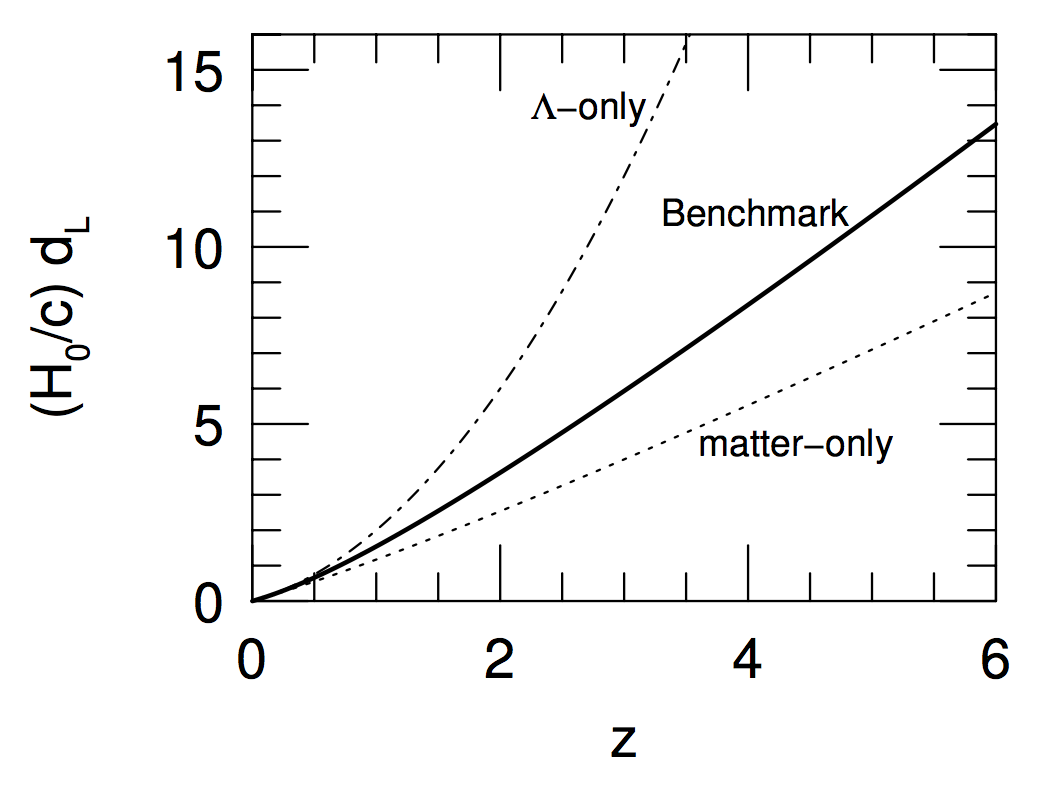
\includegraphics[width=12cm]{figures/cosmology/LuminosityDistance.png}}
\end{figure}

{\noindent}Figure \ref{fig:luminositydistance} shows the luminosity distance $d_L$ as a function of redshift $z$ for the Benchmark Model, and for two other flat Universes, one dominated by matter and one dominated by a cosmological constant $\Lambda$. When $z \ll 1$, the current proper distance may be approximated as

\begin{align*}
    d_p(t_0) \approx \frac{c}{H_0}z \left(1-\frac{1+q_0}{2}z\right) ~ [{\rm Mpc}].
\end{align*}

{\noindent}In a universe which is nearly flat, the luminosity distance may thus be approximated as

\begin{align*}
    d_L &\approx \frac{c}{H_0}z \left(1-\frac{1+q_0}{2}z\right)(1+z) \\
        & \approx \frac{c}{H_0}z \left(1+\frac{1-q_0}{2}z\right).
\end{align*}

{\noindent}Note that in the limit $z\rightarrow0$,

\begin{align*}
    d_p(t_0) \approx d_L \approx \frac{c}{H_0}z ~ [{\rm Mpc}].
\end{align*}

{\noindent}In a universe described by the Robertson-Walker metric, the luminosity distance is a good approximation to the current proper distance for objects with small redshifts.

{\noindent}Substituting the luminosity distance approximation into the expression for the distance modulus gives us the relation between distance modulus and redshift:

\begin{align*}
    m - M \approx 43.17 - 5\log_{10} \left(\frac{H_0}{70\,{\rm km\,s^{-1}\,Mpc}}\right) + 5\log_{10}z + 1.086(1-q_0)z ~ [{\rm mag}].
\end{align*}

{\noindent}For a population of standard candles with known luminosity $L$ (and hence of known bolometric absolute magnitude $M$), you measure the flux $F$ (or equivalently, the bolometric apparent magnitude $m$) and the redshift $z$. In the limit $z\rightarrow0$, a plot of $m − M$ versus $log_{10}(z)$ gives a straight line whose amplitude at a given value of $z$ tells you the value of $H_0$. At slightly larger values of $z$, the deviation of the plot from a straight line tells you the value of $q_0$. At a given value of $z$, an accelerating universe (with $q_0<0$) yields standard candles with a smaller flux than would a decelerating universe (with $q_0>0$).

\begin{figure*}[h!]
    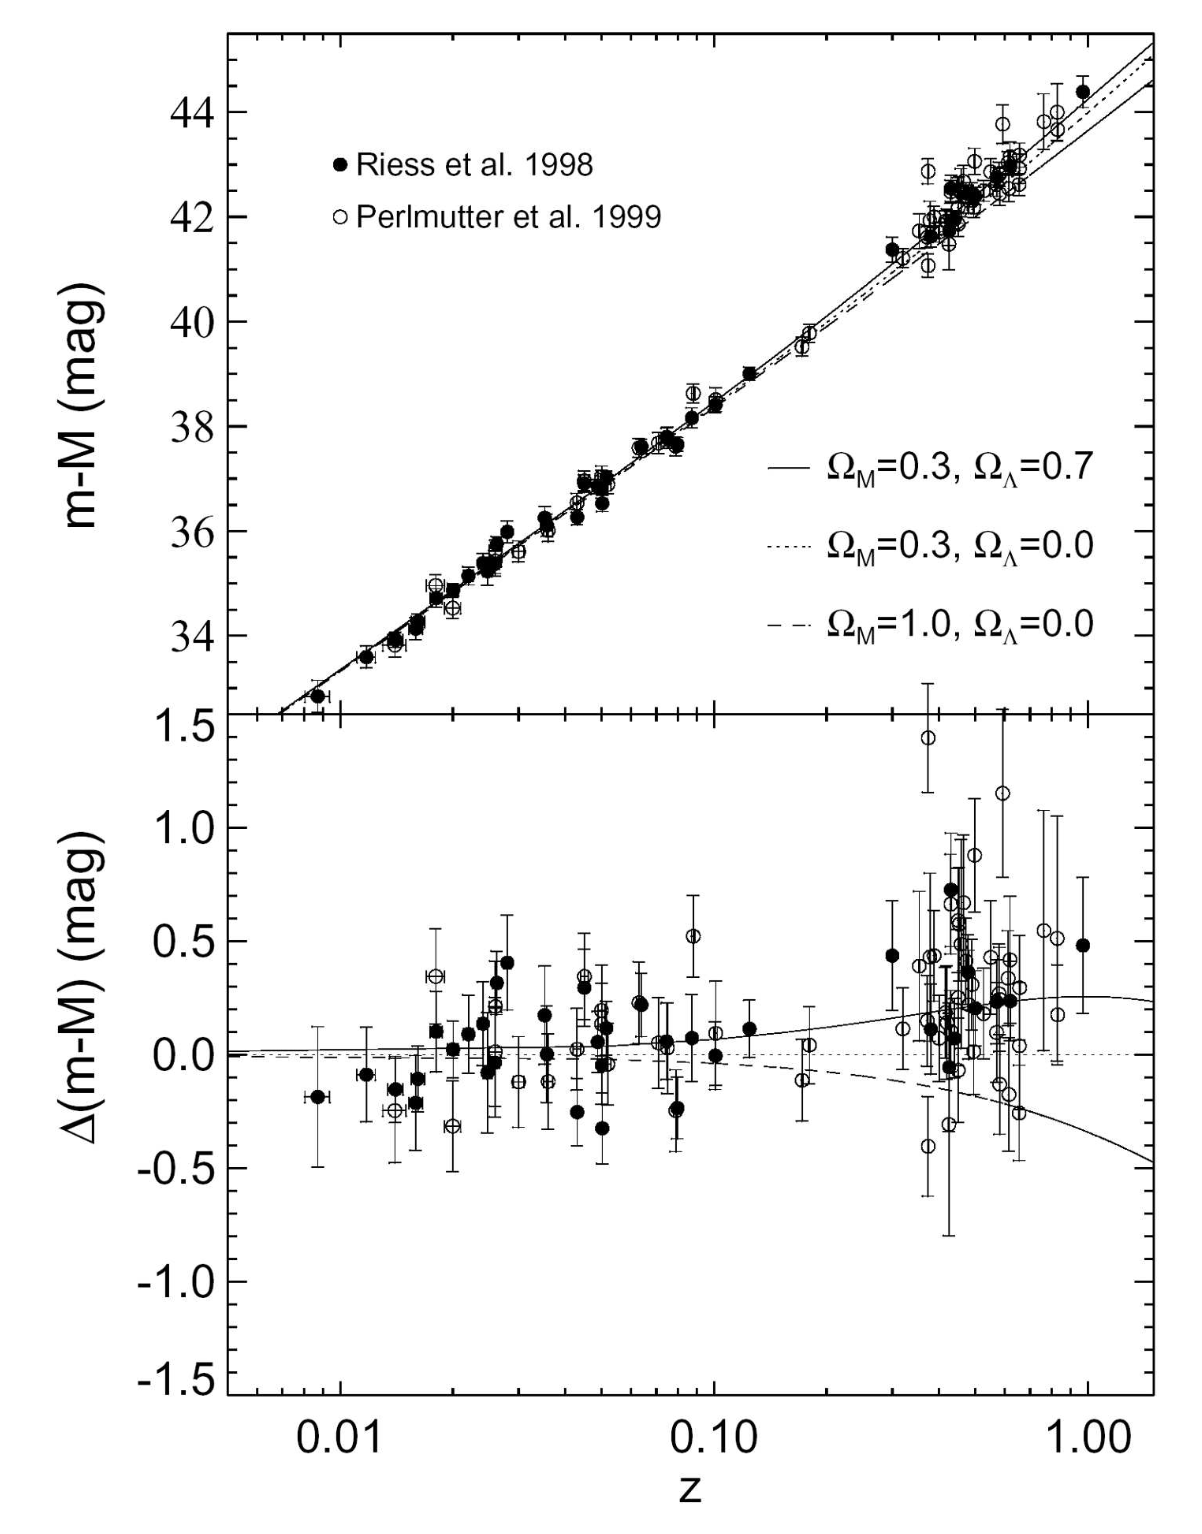
\includegraphics[width=15cm]{figures/cosmology/DistanceModulus.png}
    \centering
    \caption{Distance modulus versus redshift for Type Ia supernovae from the Supernova Cosmology Project (Perlmutter et al. 1999, ApJ, 517, 565) and the High-z Supernova Search Team (Riess et al. 1998, AJ, 116, 1009). The bottom panel shows the difference between the data and the predictions of a negatively curved $\Omega_{m,0}=0.3$ model (from Riess 2000, PASP, 112, 1284). Figure taken from Ryden (2006).}
    \label{fig:distancemodulus}
\end{figure*}

{\noindent}The upper panel of Figure \ref{fig:distancemodulus} shows the plot of distance modulus versus redshift for the combined supernova samples of the High-z Supernova Search Team (given by the filled circles) and the Supernova Cosmology Project (given by the open circles). The observational results are compared to the expected results for three model Universes. One Universe is flat, and contains nothing but matter $(\Omega_{m,0}=1, q_0=0.5)$. The second is negatively curved, and contains nothing but matter $(\Omega_{m,0}=0.3, q_0=0.15)$. The third is flat, and contains both matter and a cosmological constant $(\Omega_{m,0}=0.3, \Omega_{\Lambda,0}=0.7, q_0=−0.55).$ The data are best fitted by the third of the models -- which is, in fact, our Benchmark Model. The bottom panel of Figure \ref{fig:distancemodulus} shows this result more clearly. It shows the difference between the data and the predictions of the negatively curved, matter-only model. The conclusion that the Universe is accelerating derives from the observation that the supernovae seen at $z \sim 0.5$ are, on average, about $0.25\,{\rm mag}$ fainter than they would in a decelerating universe with $\Omega_{m,0}=0.3$ and no cosmological constant.
 
\begin{figure}[h]
    \floatbox[{\capbeside\thisfloatsetup{capbesideposition={right,top},capbesidewidth=4cm}}]{figure}[\FBwidth]
    {\caption{\footnotesize{The values of $\Omega_{m,0}$ (horizontal axis) and $\Omega_{\Lambda,0}$ (vertical axis) which best fit the data shown in Figure \ref{fig:distancemodulus}. The solid ovals show the best-fitting values for the High-z Supernova Search Team data; the dotted ovals show the best-fitting values for the Supernova Cosmology Project data (from Riess 2000, PASP, 112, 1284) Figure taken from Ryden (2006).}}
    \label{fig:omegamodel}}
    {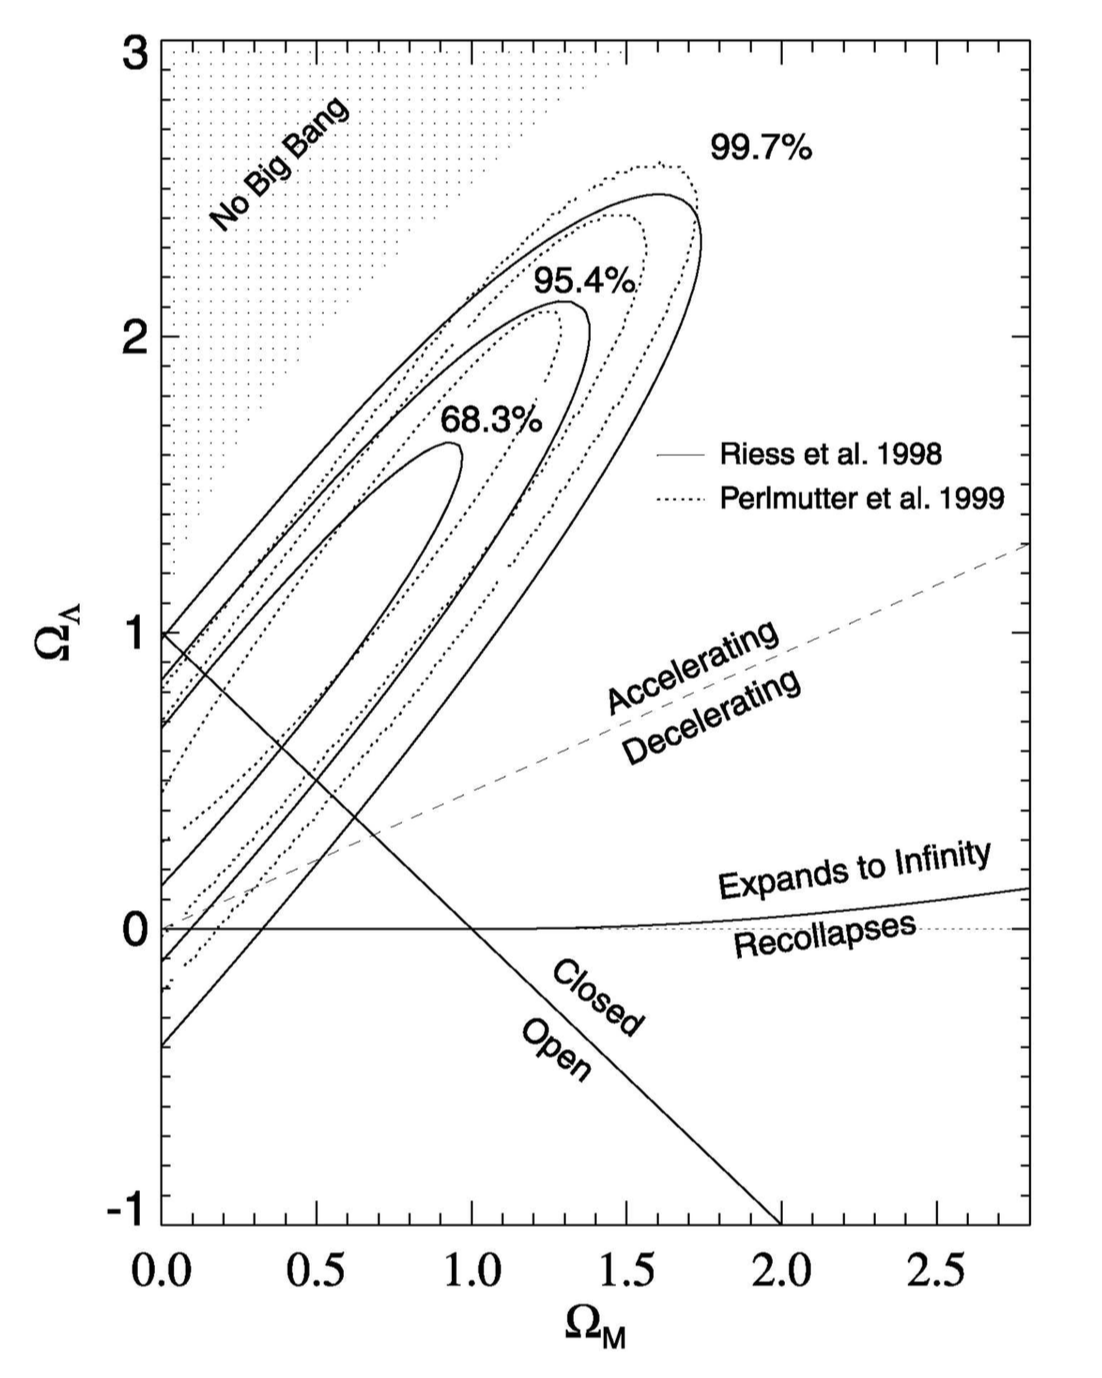
\includegraphics[width=12cm]{figures/cosmology/OmegaModel.png}}
\end{figure}

{\noindent}The supernova data extend out to $z\sim1$; this is beyond the range where an expansion in terms of $H_0$ and $q_0$ is adequate to describe the scale factor $a(t)$. Thus, the two supernova teams customarily describe their results in terms of a model universe which contains both matter and a cosmological constant. After choosing values of $\Omega_{m,0}$ and $\Omega_{\Lambda,0}$, they compute the expected relation between $m − M$ and $z$, and compare it to the observed data. The results of fitting these model universes are given in Figure \ref{fig:omegamodel}. The ovals drawn on Figure \ref{fig:omegamodel} enclose those values of $\Omega{m,0}$ and $\Omega_{\Lambda,0}$ which give the best fit to the supernova data. The results of the two teams (the solid ovals and dotted ovals) give very similar results. Three concentric ovals are shown for each team’s result; they correspond to $1\sigma$, $2\sigma$, and $3\sigma$ confidence intervals, with the inner oval representing the highest probability. The best fitting models lie along the line $0.8\Omega{m,0} − 0.6\Omega_{\Lambda,0}≈ −0.2.$ Note that decelerating universes (with $q_0>0$) can be strongly excluded by the data, as can Big Crunch universes (labeled `Recollapses' in Figure \ref{fig:omegamodel}), and Big Bounce universes (labeled `No Big Bang' in Figure \ref{fig:omegamodel}). The supernova data are consistent with negative curvature (labeled `Open' in Figure \ref{fig:omegamodel}), positive curvature (labeled `Closed' in Figure \ref{fig:omegamodel}), or with a Universe which is spatially flat.

{\noindent}The results of the supernova teams made headlines when they were first announced; the discovery of the accelerating Universe was named by Science magazine as the `Scientific Breakthrough of the Year' for 1998. It is prudent to remember, however, that all the hoopla about the accelerating Universe is based on the observation that Type Ia supernova at $z\sim.5$ and beyond have somewhat lower fluxes (by about 25\%) than they would have in a decelerating Universe. There are other reasons why their fluxes might be low. For instance, if Type Ia supernovae were intrinsically less luminous at $z\sim0.5$ than at $z\sim0$, that could explain their low fluxes. (If a typical supernova at $z\sim0.5$ had $L=3\times10^9\mathrm{L}_\odot$ rather than $L=4\times10^9\mathrm{L}_\odot$, that would explain their observed dimness, without the need to invoke a cosmological constant. Conversely, if the typical supernova at $z\sim0.5$ had $L=5\times10^9\mathrm{L}_\odot$ rather than $L=4\times10^9\mathrm{L}_\odot$, that would require an even larger cosmological constant to explain their observed dimness.) However, the other properties of Type Ia supernovae, such as their spectra, don’t seem to evolve with time, so why should their luminosity? Perhaps the fluxes of supernovae at $z\sim0.5$ are low because some of their light is scattered or absorbed by intervening dust. However, dust tends to scatter some wavelengths of light more than others. This would change the shape of the spectrum of distant Type Ia supernovae, but no dependence of spectral shape on redshift is observed.

{\noindent}In sum, the supernova results of Figure \ref{fig:omegamodel} provide persuasive evidence for a nearly flat accelerating Universe with $\Omega{m,0}\approx0.3$ and $\Omega_{\Lambda,0}≈ 0.7$.

\subsubsection{Follow-up Questions}

\begin{itemize}
    \item What are Type Ia supernovae (i.e., what is physically happening)?
    \item Can Type Ia constrain all cosmological parameters?
    \item What are some sources of error?
\end{itemize}

% --------------------------------------------------------------
%
%                           8. 
%
% --------------------------------------------------------------

\newpage
\subsection{Question 8}

Describe two methods, other than Type Ia supernovae, by which the cosmological parameters can be determined by astronomical observations.

\subsubsection{Short answer}

Short answer.

\subsubsection{Additional context}

\textbf{CMB Angular Power Spectrum}:

{\noindent}The cosmic microwave background consists of photons that last interacted with matter at $z\sim1,100$. Since the Universe must already have been inhomogeneous at this time, in order for the structures present in the current Universe to be able to form, it is expected that these spatial inhomogeneities are visible as a (small) anisotropy of the CMB: \textit{the angular distribution of the CMB temperature reflects the matter inhomogeneities at the redshift of decoupling of radiation and matter}. The CMB anisotropies reflect the conditions in the Universe at the epoch of recombination, thus at $z\sim1,100$. Temperature fluctuations originating at this time are called \textbf{primary anisotropies}. Later, as the CMB photons propagate through the Universe, they may experience a number of distortions along their way which, again, may change their temperature distribution on the sky. These effects then lead to \textbf{secondary anisotropies}.

{\noindent}Of the primary anisotropies (which directly pertain to inhomogeneities at the time of last scattering) the most basic mechanisms can be divided into those which occur on scales larger than the horizon size at recombination, i.e., which can not have been affected by physical interactions up to the time of last scattering, and those on smaller scales. The effects on superhorizon scales are the following:

\begin{itemize}
    \item \textbf{Sachs-Wolfe effect}: Inhomogeneities in the gravitational potential cause photons which originate in regions of higher density to climb out of a potential well. As a result of this, they lose energy and are redshifted (\textbf{gravitational redshift}). This effect is partly compensated for by the fact that, besides the gravitational redshift, a gravitational time delay also occurs: a photon that originates in an overdense region will be scattered at a slightly earlier time, and thus at a slightly higher temperature of the Universe, compared to a photon from a region of average density. Both effects always occur side by side. This results in photons that are cooler in baryon overdensities. (The dominant one at superhorizon scales.)
    \item \textbf{Peculiar velocities}: The electrons that scatter the CMB photons for the last time do not follow exactly the Hubble expansion, but have an additional velocity that is closely linked to the density fluctuations. This results in a Doppler effect: if photons are scattered by gas receding from us with a speed larger than that corresponding to the Hubble expansion, these photons experience an additional redshift which reduces the temperature measured in that direction.
    \item \textbf{Enhanced baryon density}: The distribution of baryons follows that of the dark matter, so that in regions of a higher dark matter density, the baryon density is also enhanced. This leads to an increased temperature of the baryons in overdense regions.
\end{itemize}

{\noindent}These three effects are relevant on scales larger than the (sound) horizon scale at the epoch of recombination. Obviously, they are closely coupled to each other. In particular, on scales $>r_\mathrm{H,com}(z_\mathrm{rec})$, the first two effects can partially compensate each other, though the Sachs–Wolfe effect is the dominant one at superhorizon scales. Inside the (sound) horizon, two other effects dominate the primary anisotropy signal:

\begin{enumerate}
    \item \textbf{Baryon acoustic oscillations}: On subhorizon scales, the pressure of the baryon-photon fluid is effective because, prior to recombination, these two components had been closely coupled by Compton scattering. This leads to sound waves in the baryon-photon fluid, called the baryonic acoustic oscillations (BAOs). In the density peaks of these sound waves, the baryon-photon fluid is adiabatically compressed and thus hotter than the average. The CMB sky yields a two-dimensional cut through this three-dimensional density (and temperature) field of these sound waves, and thus reflect these fluctuations, yielding temperature anisotropies with characteristic length (or angular) scales. (More on this later.)
    \item \textbf{Silk damping}: The coupling of baryons and photons is not perfect since, owing to the finite mean free path of photons, the two components are decoupled on small spatial scales. This implies that on small length-scales, the temperature fluctuations can be smeared out by the diffusion of photons. This process is known as \textbf{Silk damping}, and it implies that on angular scales below about $\sim50'$, only very small primary fluctuations exist.
\end{enumerate}

{\noindent}\textbf{BAOs}: On subhorizon scales, the pressure of the baryon-photon fluid is effective because, prior to recombination, these two components had been closely coupled by Compton scattering. This leads to sound waves in the baryon-photon fluid, called the baryonic acoustic oscillations (BAOs). In the density peaks of these sound waves, the baryon-photon fluid is adiabatically compressed and thus hotter than the average. The CMB sky yields a two-dimensional cut through this three-dimensional density (and temperature) field of these sound waves, and thus reflect these fluctuations, yielding temperature anisotropies with characteristic length (or angular) scales. 

{\noindent}We expect that these frozen sound waves of the baryons leave an imprint on the overall matter correlation function, best seen in Figure \ref{fig:perturbationevolution}. This unique feature in the correlation function, if it can be detected in the galaxy correlation function, would provide a well-defined `standard rod' in the observable Universe. Since we can observe only angular scales on the sky, the relation between the (comoving) length of the standard rod and the associated angular scale provides a measure of distance. Therefore, a measurement of the baryonic acoustic oscillations (BAOs) in the correlation of galaxies at a given redshift $z$ can be used to determine the (comoving) angular diameter distance $d_A(z)$ --  which depends on the density parameters $\Omega_m$ and $\Omega_\Lambda$.

{\noindent}In fact, the three-dimensional correlation function does not only depend on the transverse length scale which is related to the angular scale via the angular-diameter distance, but also on the separation of galaxies along the line-of-sight. The comoving distance interval corresponding to a redshift interval $\Delta z$ is given by $\Delta x=c\Delta z/H(z)$. Since there are two transversal dimensions, and one along the line-of-sight, the distance measure that is determined best from BAOs is the geometric mean

\begin{align*}
    D(z) = \left(d_A^2(z)\frac{cz}{H(z)}\right)^{1/3}.
\end{align*}

{\noindent}The large redshift surveys 2dFGRS and SDSS allowed the first detection of these BAOs in the galaxy distribution in 2005. Figure \ref{fig:correlationfunction} shows the discovery of BAOs from the SDSS, where a clear feature in the galaxy correlation function is seen at the expected length scale. The mean redshift of the galaxies from which the correlation function was determined is $z\sim0.35$; thus, this measurement yields an estimate of the angular diameter distance to that redshift, with about a 5\% accuracy. In particular, we point out that the sound horizon at recombination is visible in the current Universe!

\begin{figure}[h]
    \floatbox[{\capbeside\thisfloatsetup{capbesideposition={right,top},capbesidewidth=4cm}}]{figure}[\FBwidth]
    {\caption{\footnotesize{The correlation function of galaxies, as observed in the SDSS, shows a clear indication of a secondary peak on a comoving scale of about $100h^{-1}\,{\rm Mpc}\sim150\,{\rm Mpc}$. Curves show models with slightly different density parameter $\Omega_mh^2 = 0.12; 0.13; 0.14$, with fixed baryon density of $\Omega_bh^2=0.024$. The lowest, smooth curve is a  CDM model without baryons which thus shows no features due to baryonic oscillations. Source: D. Eisenstein et al. 2005, Detection of the Baryon Acoustic Peak in the Large-Scale Correlation Function of SDSS Luminous Red Galaxies, ApJ 633, 560, p. 563, Fig. 2. Figure taken from Schneider (2006).}}
    \label{fig:correlationfunction}}
    {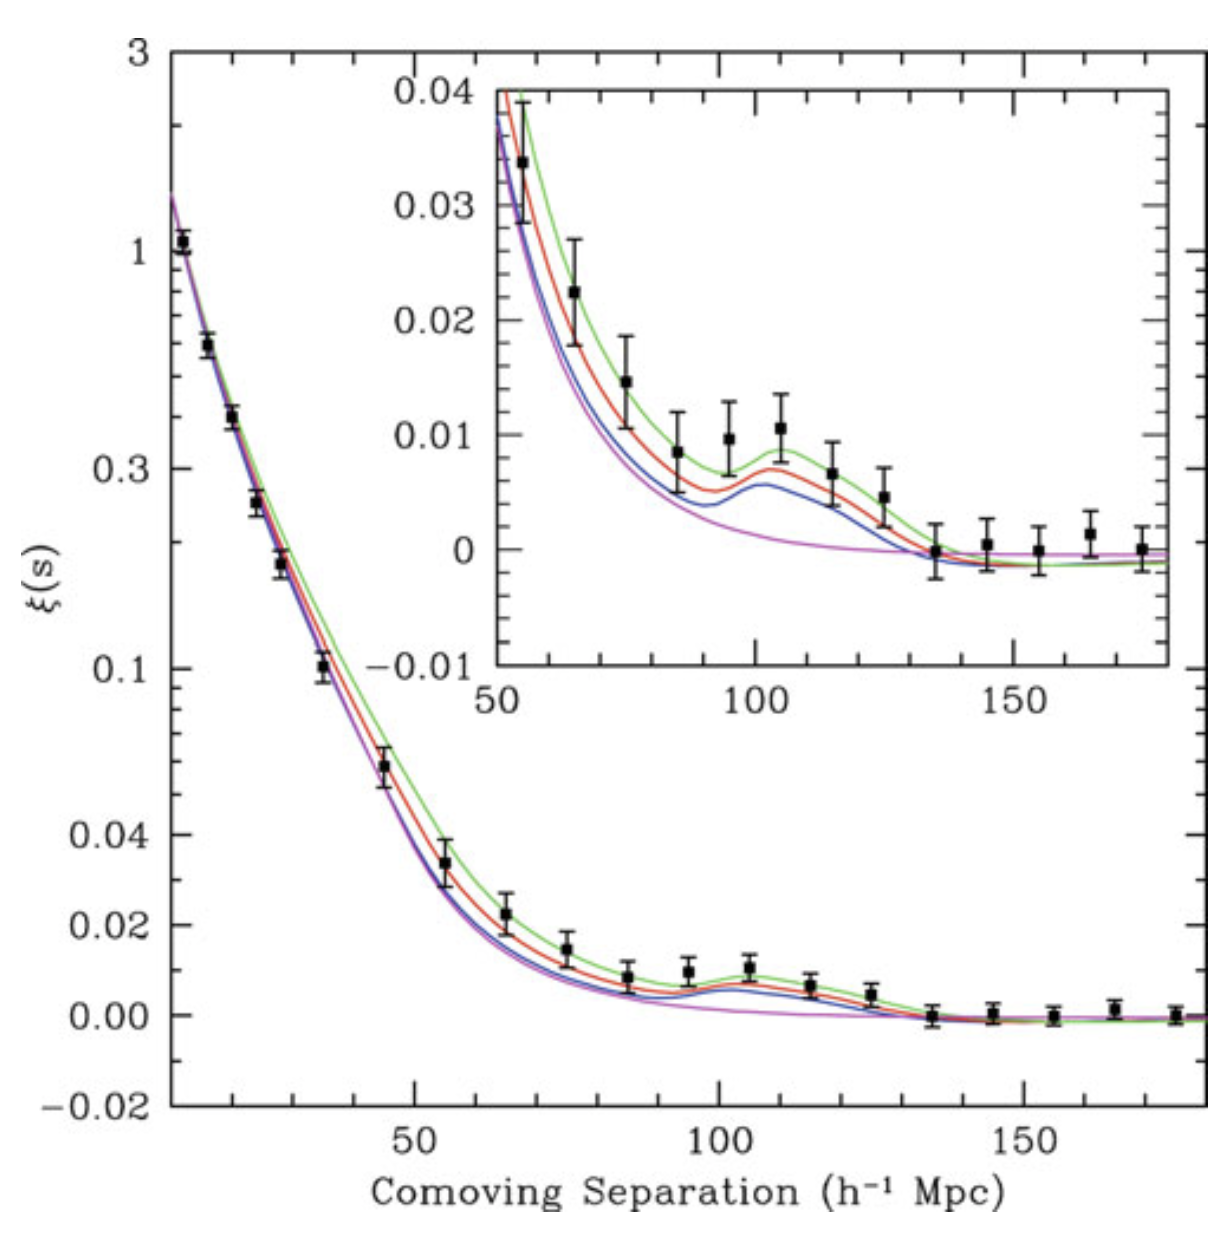
\includegraphics[width=12cm]{figures/cosmology/CorrelationFunction.png}}
\end{figure}

{\noindent}The power of the method depends on whether the galaxies trace the underlying matter distribution sufficiently well, so that the measured galaxy correlation function reflects the correlation function of matter. Given the large spatial scale on which BAOs are observed, the proportionality between the galaxy and matter fluctuation fields, assumed by the simple bias model, is expected to hold very well. This then turns BAOs into a straightforward, almost purely geometrical tool for measuring the geometry of our Universe.

{\noindent}For this reason, several surveys are underway to measure the acoustic scale as a function of redshift. Figure \ref{fig:BAOs} shows recent measurements of BAOs over a range of redshifts. Amazingly, the measurements are in perfect agreement with the cosmological parameters as determined by CMB anisotropy measurements. In particular, the spatial flatness of our Universe is confirmed, and any curvature is constrained to be very small, $\lvert\Omega_m+\Omega_\Lambda\rvert\lesssim0.01$.

\begin{figure*}[t]
    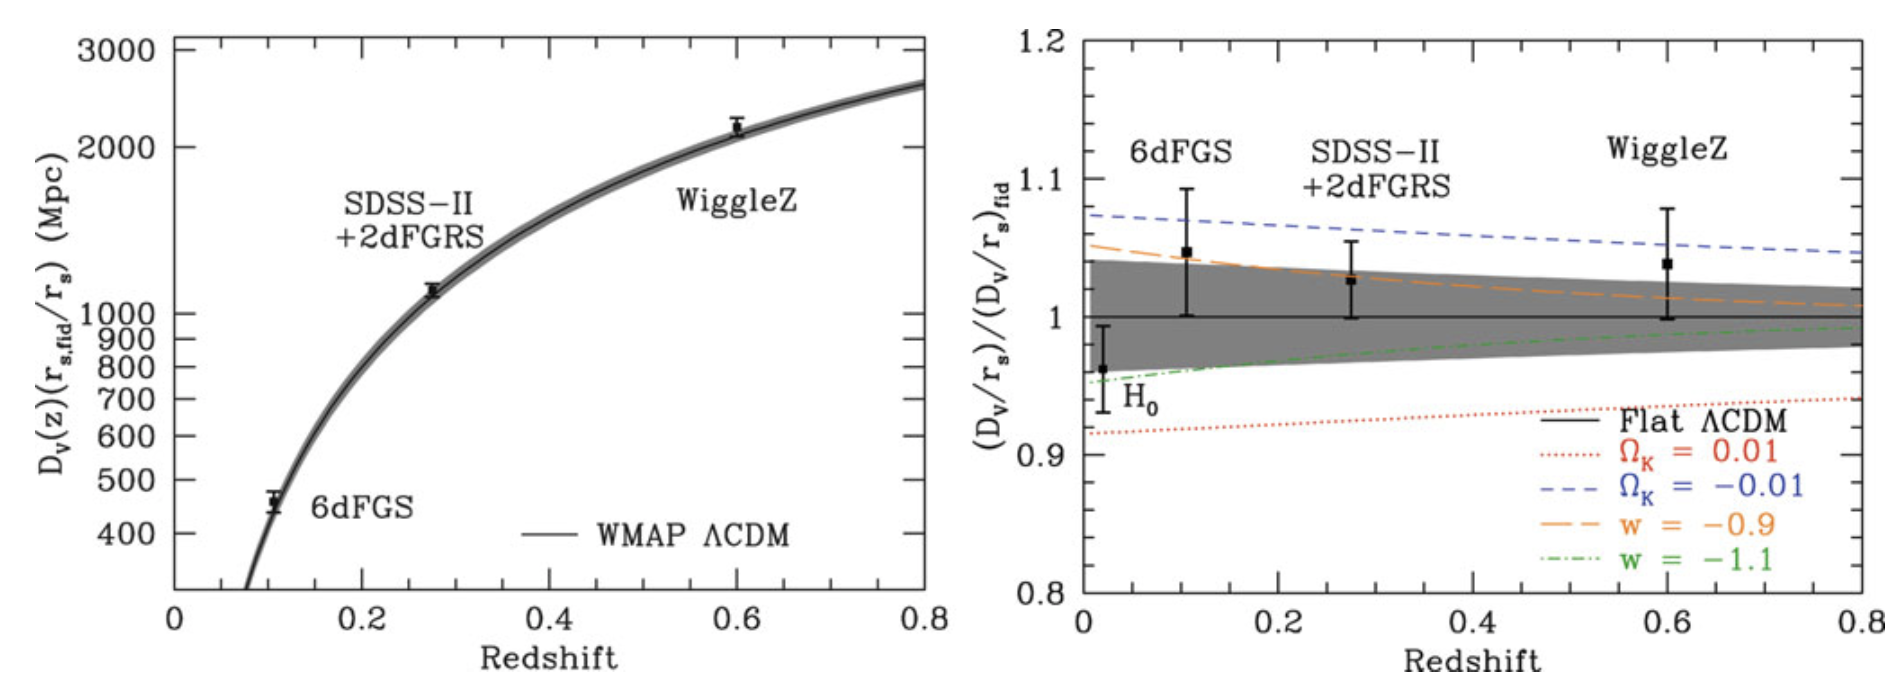
\includegraphics[width=16cm]{figures/cosmology/BAOs.png}
    \centering
    \caption{\footnotesize{Recent results on the distance-redshift relation from measurements of BAOs. Left panel: The black line and the grey band shows the best-fit cosmological model obtained from the WMAP CMB anisotropy measurements and its $1\sigma$  uncertainty range. The BAO distance determination from three surveys are indicated, which are located right on this best-fit model. Right panel: The same data are shown, now divided by the prediction of a flat $\Lambda$CDM model with parameters as determined from WMAP. Also shown are curves of this distance ratio for models with a small positive or negative curvature, or for different equations-of-state of dark energy. In particular, the BAO measurements exclude any appreciable curvature parameter of our Universe. Source: D.H. Weinberg et al. 2012, Observational Probes of Cosmic Acceleration, arXiv:1201.2434, Fig. 8. Figure taken from Schneider (2006).}}
    \label{fig:BAOs}
\end{figure*}

% --------------------------------------------------------------
%
%                           9. 
%
% --------------------------------------------------------------

\newpage
\subsection{Question 9}

Why is the cosmic microwave background expected to be weakly polarized, and what is practically required to observe this signal?

\subsubsection{Short answer}

The CMB is linearly polarized at the 10\% level due to Thomson scattering of photons off of free electrons at the surface of last scattering.  The degree of linear polarization is directly related to the quadrupole anisotropy in the photons when they last scatter. If the incoming radiation field were isotropic, orthogonal polarization states from incident directions would balance so that the outgoing radiation would remain unpolarized. Conversely, if the incident radiation field possesses a quadrupolar variation in intensity or temperature (which possess intensity peaks at $90^\circ=\pi/2$ separations), the result is a linear polarization of the scattered radiation. No other multipoles other than the quadrupole contributes to the CMB polarization!

\subsubsection{Additional context}

{\noindent}Why should we be concerned with the polarization of the cosmic microwave background (CMB) anisotropies? That the CMB anisotropies are polarized is a fundamental prediction of the gravitational instability paradigm. Under this paradigm, small fluctuations in the early universe grow into the large scale structure we see today. If the temperature anisotropies we observe are indeed the result of primordial fluctuations, their presence at last scattering would polarize the CMB anisotropies themselves. The verification of the (partial) polarization of the CMB on small scales would thus represent a fundamental check on our basic assumptions about the behavior of fluctuations in the Universe, in much the same way that the redshift dependence of the CMB temperature is a test of our assumptions about the background cosmology. Furthermore, observations of polarization provide an important tool for reconstructing the model of the fluctuations from the observed power spectrum (as distinct from fitting an a priori model prediction from observations). The polarization probes the epoch of last scattering directly as opposed to the temperature fluctuations which may evolve between last scattering and the present. This localization in time is a very powerful constraint for reconstructing the sources of anisotropy. Moreover, different sources of temperature anisotropies (scalar, vector, and tensor) give different patterns in the polarization: both in its intrinsic structure and in its correlation with the temperature fluctuations themselves. Thus by including polarization information, one can distinguish the ingredients which go to make up the temperature power spectrum and so the cosmological model. Finally, the polarization power spectrum provides information complementary to the temperature power spectrum even for ordinary (scalar or density) perturbations. This can be of use in breaking parameter degeneracies and thus constraining cosmological parameters more accurately. The prime example of this is the degeneracy, within the limitations of cosmic variance, between a change in the normalization and an epoch of ``late'' reionization.

{\noindent}Yet how polarized are the fluctuations? The degree of linear polarization is directly related to the quadrupole anisotropy in the photons when they last scatter. While the exact properties of the polarization depend on the mechanism for producing the anisotropy, several general properties arise. The polarization peaks at angular scales smaller than the horizon at last scattering due to causality. Furthermore, the polarized fraction of the temperature anisotropy is small since only those photons that last scattered in an optically thin region could have possessed a quadrupole anisotropy. The fraction depends on the duration of last scattering. For the standard thermal history, it is 10\% on a characteristic scale of tens of arcminutes. Since temperature anisotropies are at the $10^{-5}$ level, the polarized signal is at (or below) the $10^{-6}$ level, or several $\mu\mathrm{K}$ representing a significant experimental challenge.

{\noindent}The Thomson scattering cross section $\sigma_T$ depends on polarization as (see, e.g., Chandrasekhar, 1960) as 

\begin{align*}
    \frac{\mathrm{d}\sigma_T}{\mathrm{d}\Omega} \propto \lvert \bm{\epsilon}\cdot\bm{\epsilon}' \rvert^2,
\end{align*}

{\noindent}where $\bm{\epsilon}$ and $\bm{\epsilon}'$ are the incident and scattered polarization directions, and $\Omega$ is the solid angle. Heuristically, the incident light sets up oscillations of the target electron in the direction of the electric field vector $E$ (i.e., the polarization). The scattered radiation intensity thus peaks in the direction normal to, with polarization parallel to, the incident polarization. More formally, the polarization dependence of the cross section is dictated by electromagnetic gauge invariance and thus follows from very basic principles of fundamental physics.

\begin{figure}[h]
    \floatbox[{\capbeside\thisfloatsetup{capbesideposition={right,top},capbesidewidth=4cm}}]{figure}[\FBwidth]
    {\caption{\footnotesize{Thomson scattering of radiation with a quadrupole anisotropy generates linear polarization. Blue colors (thick lines) represent hot and red colors (thin lines) cold radiation. Figure taken from Hu \& White (1997).}}
    \label{fig:Thomsonscattering}}
    {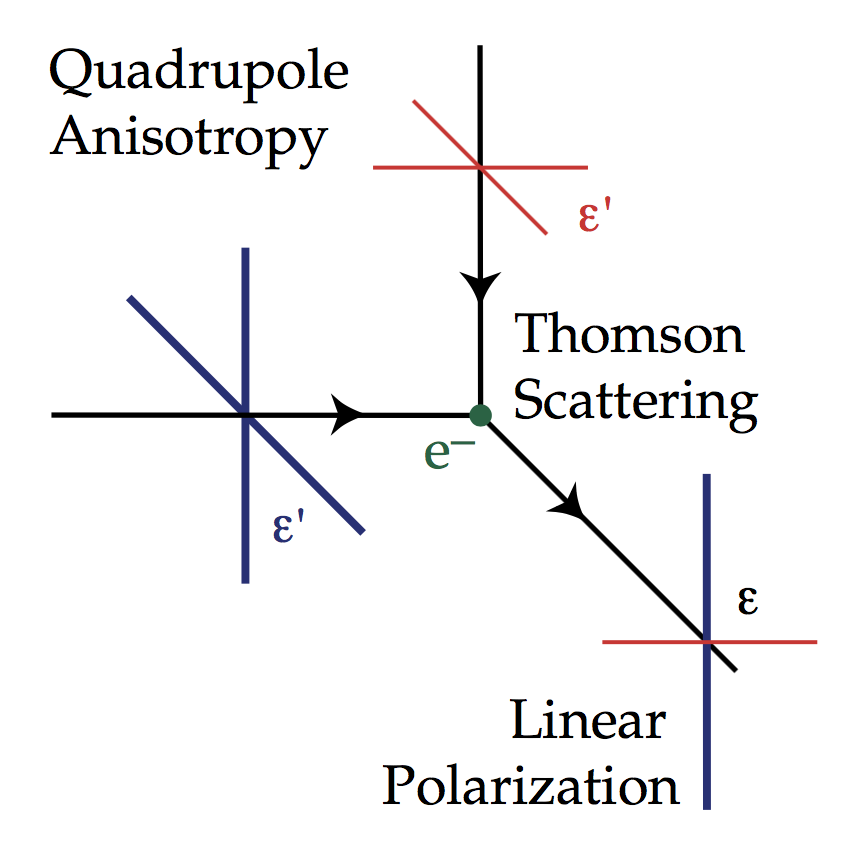
\includegraphics[width=12cm]{figures/cosmology/ThomsonScattering.png}}
\end{figure}

{\noindent}If the incoming radiation field were isotropic, orthogonal polarization states from incident directions separated by $90^\circ$ would balance so that the outgoing radiation would remain unpolarized. Conversely, if the incident radiation field possesses a quadrupolar variation in intensity or temperature (which possess intensity peaks at $90^\circ=\pi/2$ separations), the result is a linear polarization of the scattered radiation (see Figure \ref{fig:Thomsonscattering}). A reversal in sign of the temperature fluctuation corresponds to a $90^\circ$ rotation of the polarization, which reflects the spin-$2$ nature of polarization.

{\noindent}In terms of a multipole decomposition of the radiation field into spherical harmonics, $Y_\ell^m(\theta,\phi)$, the five quadrupole moments are represented by $\ell= 2, m=O,\pm1,\pm2$. The orthogonality of the spherical harmonics guarantees that no other moment can generate polarization from Thomson scattering. In these spherical coordinates, with the north pole at $\theta=0$, we call a N-S (E-W) polarization component $Q>0$ ($Q<0$) and a NE-SW (NW-SE) component $U>0$ ($U<0$). The polarization amplitude and angle clockwise from north are

\begin{align*}
    P = \sqrt{Q^2+U^2}
\end{align*}

{\noindent}and

\begin{align*}
    \chi = \frac{1}{2}\arctan\left(\frac{U}{Q}\right).
\end{align*}

{\noindent}where $P$ is the polarized intensity and $Q$ and $U$ are the linear polarization Stokes vectors.

{\noindent}If Thomson scattering is rapid, then the randomization of photon directions that results destroys any quadrupole anisotropy and polarization. The problem of understanding the polarization pattern of the CMB thus reduces to understanding the quadrupolar temperature fluctuations at last scattering. Temperature perturbations have 3 geometrically distinct sources: the scalar (compressional), vector (vertical) and tensor (gravitational wave) perturbations. Formally, they form the irreducible basis of the symmetric metric tensor. We shall consider each of these below and show that the scalar, vector, and tensor quadrupole anisotropy correspond to $m=0,\pm1,\pm2$ respectively. This leads to different patterns of polarization for the three sources.

\subsubsection{Follow-up Questions}

\begin{itemize}
    \item What are some foregrounds or challenges to observing this signal?
    \item Why does dust polarize the CMB?
    \item Why is dust not randomly oriented?
    \item How did we first determine that dust is not randomly oriented?
\end{itemize}

% --------------------------------------------------------------
%
%                           10. 
%
% --------------------------------------------------------------

\newpage
\subsection{Question 10}

Our view of the cosmic microwave background is affected by what is along the line of sight. Give two examples of CMB foregrounds that also provide information about the cosmic parameters.

\subsubsection{Short answer}

Short answer.

\subsubsection{Additional context}

{\noindent}\textbf{The thermal Sunyaev-Zeldovich effect}: 

{\noindent}Given that the amplitude of the polarization is so small the question of foregrounds is even more important than for the temperature anisotropy. Unfortunately, the level and structure of the various foreground polarization in the CMB frequency bands is currently not well known. Atmospheric emission is believed to be negligibly polarized, leaving the main astrophysical foregrounds: free-free, synchrotron, dust, and point source emissions. Of these the most important foreground is synchrotron emission.

{\noindent}Free-free emission (bremsstrahlung) is intrinsically unpolarized but can be partially polarized by Thomson scattering within the HII region. This small effect is not expected to polarize the emission by more than 10\%. The emission is larger at low frequencies but is not expected to dominate the polarization at any frequency.

{\noindent}The polarization of dust is not well known. In principle, emission from dust particles could be highly polarized, however it's been found that that the majority of dust is polarized at the $\approx2\%$ level at $100\mu{\rm m}$ with a small fraction of regions approaching 10\% polarization. It's also been shown that even at 100\% polarization, extrapolation of the IRAS $100\mu{\rm m}$ map with the COBE FIRAS index shows that dust emission is negligible below $80\,{\rm GHz}$. At higher frequencies it will become the dominant foreground.

{\noindent}Radio point sources are polarized due to synchrotron
emission at $<20\%$ level. For large angle experiments, the random contribution from point sources will contribute negligibly, but may be of more concern for the upcoming satellite missions.

{\noindent}Galactic synchrotron emission is the major concern. It is potentially highly polarized with the fraction dependent on the spectral index and depolarization from Faraday rotation and non-uniform magnetic fields. The level of polarization is expected to lie between 10\%-75\% of a total intensity which itself is approximately $5\,\mu{\rm K}$ at $30\,{\rm GHz}$. This estimate follows from extrapolating measurements at $1411\,{\rm MHz}$ with an index of $T\propto\nu^{-3}$.

{\noindent}Due to their different spectral indices, the minimum
in the foreground polarization, like the temperature, lies near $100\,{\rm GHz}$. For full sky measurements, since synchrotron emission is more highly polarized than dust, the optimum frequency at which to measure intrinsic (CMB) polarization is slightly higher than for the anisotropy. Over small regions of the sky where one or the other of the foregrounds is known a priori to be absent the optimum frequency would clearly be different. However as with anisotropy measurements, with multi-frequency coverage, polarized foregrounds can be
removed.

{\noindent}It is also interesting to consider whether the spatial as well as frequency signature of the polarization can be used to separate foregrounds. Using angular power spectra for the spatial properties of the foregrounds is a simple generalization of methods already used in anisotropy work. For instance, in the case of synchrotron emission, if the spatial correlation in the polarization follows that of the temperature itself, the relative contamination will decrease on smaller angular scales due to its diffuse nature. Furthermore the peak of the cosmic signal in polarization occurs at even smaller angular scales than for the anisotropy.

{\noindent}Of those that can provide information about the cosmic parameters...

{\noindent}\textbf{The thermal Sunyaev–Zeldovich effect}: Electrons in the hot gas of the intracluster medium (ICM) can inverse Compton scatter photons of the CMB. The optical depth and thus the scattering probability for this inverse Compton scattering is relatively low, but the effect is nevertheless observable and, in addition, is of great importance for the analysis of clusters. A photon moving through a cluster of galaxies towards us will change its direction through scattering and thus will not reach us. But since the cosmic background radiation is isotropic, for any CMB photon that is scattered out of the line-of-sight, another photon exists -- statistically -- that is scattered into it, so that the total number of photons reaching us is preserved. However, the energy of the photons changes slightly through scattering by the hot electrons, in a way that they have an (on average) higher frequency after scattering. Hence, by this inverse Compton scattering, energy is on average transferred from the electrons to the photons, as can be seen in Figure \ref{fig:szeffect}.

\begin{figure}[h]
    \floatbox[{\capbeside\thisfloatsetup{capbesideposition={right,top},capbesidewidth=4cm}}]{figure}[\FBwidth]
    {\caption{\footnotesize{The influence of the Sunyaev–Zeldovich effect on the cosmic background radiation. The dashed curve represents the Planck distribution of the unperturbed CMB spectrum, the solid curve shows the spectrum after the radiation has passed through a cloud of hot electrons. The magnitude of this effect, for clarity, has been very much exaggerated in this sketch. Source: Carlstrom et al. 2002, ARA\&A 40, 643. Image taken from Schneider (2006).}}
    \label{fig:szeffect}}
    {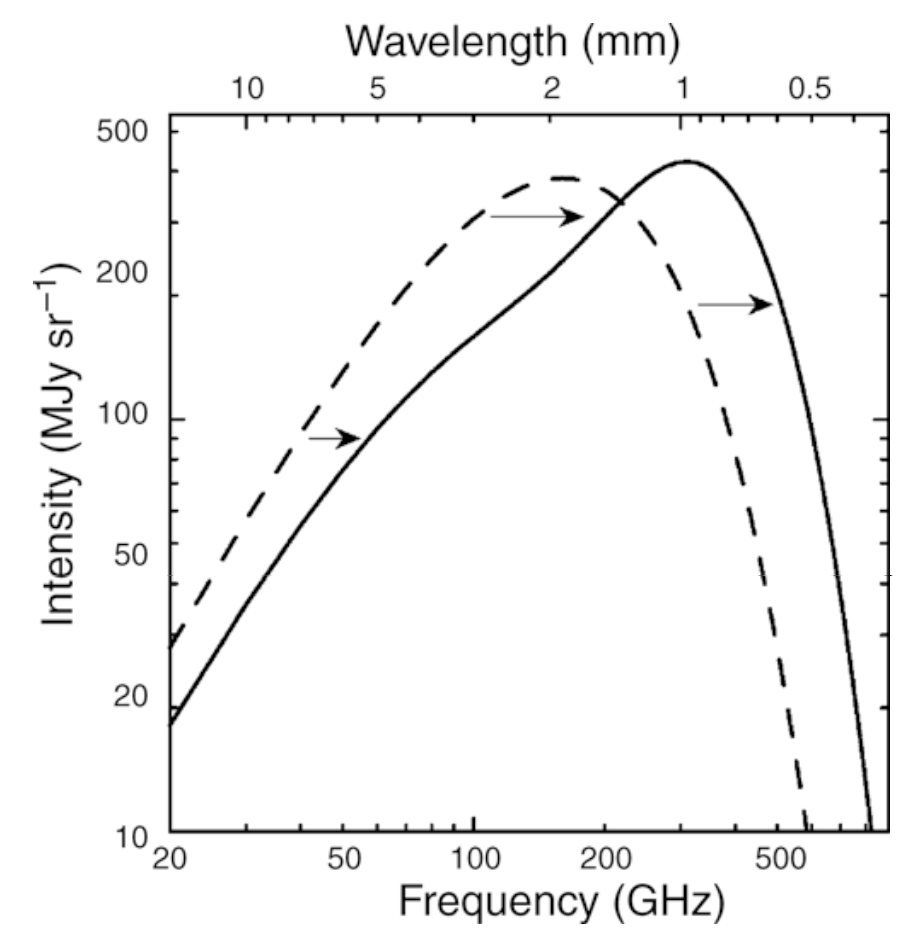
\includegraphics[width=8cm]{figures/cosmology/SZeffect.png}}
\end{figure}

{\noindent}In the Rayleigh–Jeans (RJ) domain of the CMB spectrum, at wavelengths larger than about $2{\rm mm}$, the intensity of the CMB is decreased by the SZ-effect. For the change in specific intensity in the RJ part, one obtains

\begin{align*}
    \frac{\Delta I_\nu^\mathrm{RJ}}{I_\nu^\mathrm{RJ}} = -2y,
\end{align*}

{\noindent}where y is the the Compton parameter

\begin{align*}
    y = \int\frac{k_BT}{m_ec^2}\sigma_Tn_e\mathrm{d}l
\end{align*}

{\noindent}and $\sigma_T$ is the Compton cross-section for electron scattering

\begin{align*}
    \sigma_T = \frac{8\pi}{3}\left(\frac{e^2}{m_ec^2}\right)^2 = \frac{8\pi}{3}e_{e,0}^2.
\end{align*}

{\noindent}Obviously, $y$ is proportional to the optical depth with respect to Compton scattering, given as an integral over $n_e\sigma_T$ along the line-of-sight. Furthermore, $y$ is proportional to the gas temperature, because that defines the average energy transfer per scattering event. Overall, $y$ is proportional to the integral over the gas pressure $P D=nk_BT$ along the line-of-sight through the cluster.

{\noindent}The SZ effect affects the temperature distribution of the CMB. Some of the photons propagating along lines-of-sight passing through clusters of galaxies or other regions of dense and hot gas are scattered by the hot electrons, resulting in a temperature change in these directions. We recall that in the direction of clusters the measured intensity of the CMB radiation is reduced at low frequencies, whereas it is increased at high frequencies. Hence, the SZ effect can be identified in the CMB data if measurements are conducted over a sufficiently large frequency range.


% --------------------------------------------------------------
%
%                           11. 
%
% --------------------------------------------------------------

\newpage
\subsection{Question 11}

Describe cosmological inflation. List at least three important observations it is intended to explain.

\subsubsection{Short answer}

Inflation can most generally be defined as a period of exponential expansion of the form

\begin{align*}
    a(t) \propto e^{Ht} ~ [{\rm dimensionless}]
\end{align*}

{\noindent}very early on in the Universe. Inflation is intended to explain the (1) horizon problem, (2) flatness problem, and (3) magnetic monopole problem. The flatness problem can be summarized by the statement, ``The universe is nearly flat today, and was even flatter in the past.'' The horizon problem can be summarized by the statement, ``The universe is nearly isotropic and homogeneous today, and was even more so in the past.'' The monopole problem can be summarized by the statement, ``The universe is apparently free of magnetic monopoles'' Inflation explains these puzzling aspects of our Universe, by flattening it, ensuring its homogeneity over large scales, and driving down the number density of magnetic monopoles which it contains. At present, there is not a consensus among cosmologists about the exact mechanism driving inflation.

\subsubsection{Additional context}

In the inflationary scenario it is presumed that at very
early times the vacuum energy density was much higher
than today, so that it dominated the Hubble expansion. Then $\dot{a}/a\approx\sqrt{\Lambda/3}$. This implies an exponential expansion of the Universe,

\begin{align*}
    a(t) \propto e^{Ht} ~ [{\rm dimensionless}]
\end{align*}

{\noindent}Obviously, this exponential expansion (or inflationary phase) cannot last forever. We assume that a phase transition took place in which the vacuum energy density is transformed into normal matter and radiation (a process called reheating), which ends the exponential expansion and after which the normal Friedmann evolution of the Universe begins.

{\noindent}At present, there is not a consensus among cosmologists about the exact mechanism driving inflation; there is no known scalar field which can drive inflation. (A skeptic might point out that there is no known fundamental scalar held at all!) Therefore, it may well be true that the idea of inflation is correct but it is driven by something other than a scalar field. Having said that, there are a number of reasons to work with scalar fields, as we will do whenever we need to specify the source of inflation. Almost all fundamental particle physics theories contain scalar fields. In fact, historically it was particle physicists studying high-energy extensions of the Standard Model (in particular GUTs) who proposed the idea of inflation driven by a scalar field as a natural byproduct of some of these extensions. Indeed, almost all current work on inflation is based on a scalar field (or sometimes two). The alternative from a particle physics point of view is to use a vector field (such as the electromagnetic potential) or a set of fermions (similar to the way condensates induce superconductivity) to drive inflation. Neither of these choices works very well, but they both complicate things severely, so we will stick to a scalar field.

\begin{figure}[h]
    \floatbox[{\capbeside\thisfloatsetup{capbesideposition={right,top},capbesidewidth=4cm}}]{figure}[\FBwidth]
    {\caption{\footnotesize{During an inflationary phase, indicated here by the gray bar, the universe expands exponentially; see (4.83). This phase comes to an end when a phase transition transforms the vacuum energy into matter and radiation, after which the universe follows the normal Friedmann expansion. Adapted from: Alan Guth 1998, The inflationary Universe, Basic Books. Figure taken from Schneider (2006).}}
    \label{fig:inflation}}
    {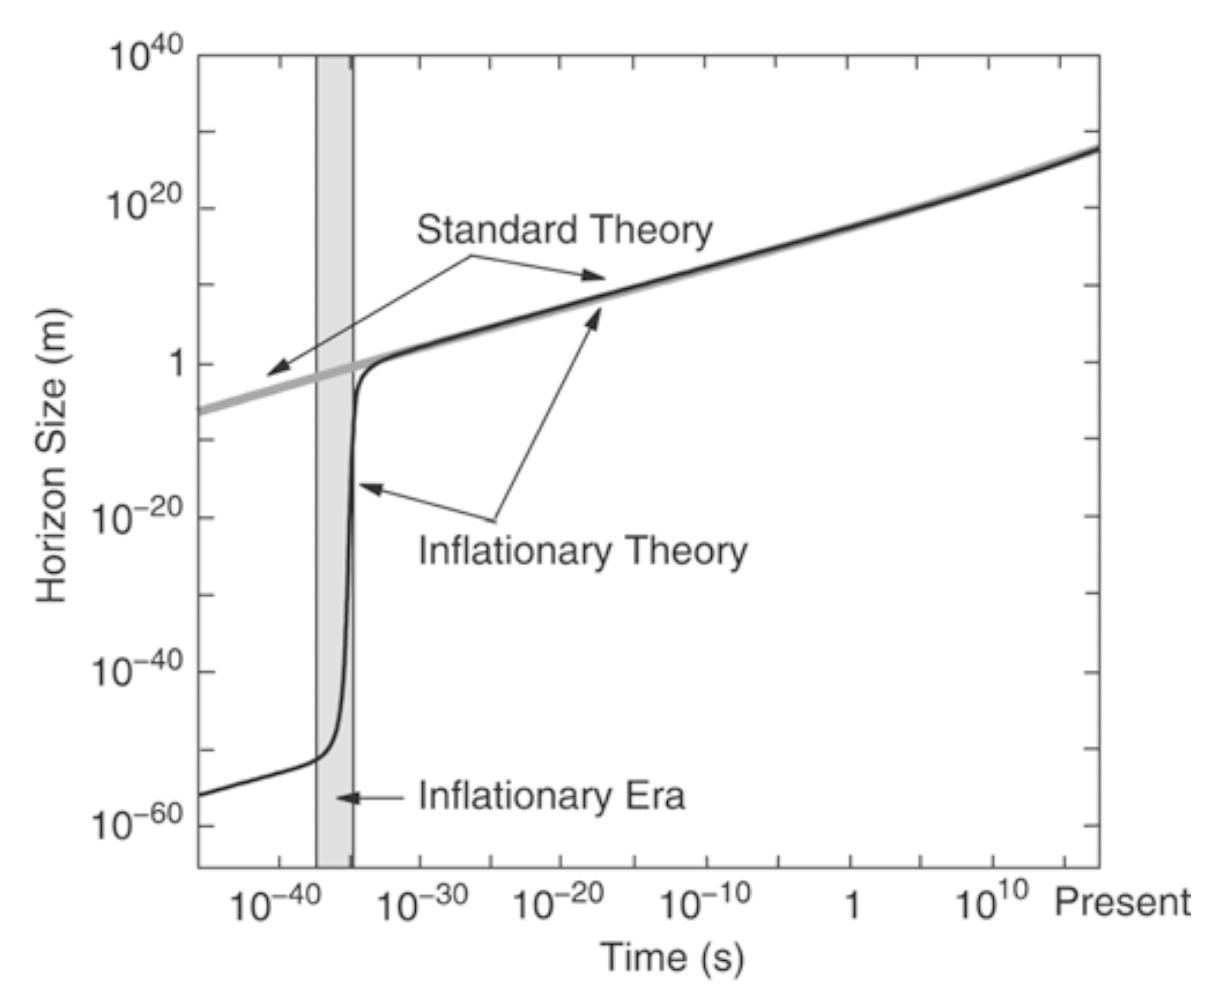
\includegraphics[width=12cm]{figures/cosmology/Inflation.png}}
\end{figure}

{\noindent}\textbf{The horizon problem}: Since no signal can travel faster than light, the existence of a horizon length means that CMB radiation from two directions separated by more than about one degree originates in regions that were not in causal contact before recombination, (i.e., the time when the CMB photons interacted with matter the last time). Therefore, these two regions have never been able to exchange information, for example about their temperature. Nevertheless their temperature is the same, as seen from the high degree of isotropy of the CMB, which shows relative fluctuations of only $\Delta T/T10^{-5}$!

{\noindent}During inflation, $H(a)=\sqrt{\Lambda/3}$ is constant so that the integral for the comoving horizon length formally diverges. This implies that the horizon may become arbitrarily large in the inflationary phase, depending on the duration of the exponential expansion. For illustration we consider a very small region in space of size $L<ct_i$ at a time $t_i\sim10^{-34}\,{\rm s}$ prior to inflation which is in causal contact. Through inflation, it expands tremendously, e.g., by a factor $10^{40}$; the original $L\sim10^{-24}\,{\rm cm}$ inflates to about $10^{16}\,{\rm cm}$ by the end of the inflationary phase, at $t_f\sim10^{-32}{\rm s}$. By today, this spatial region will have expanded by another factor of $10^{25}$ by following (for $t>t_f$) the normal cosmic expansion, to   $10^{41}\,{\rm cm}$. This scale is considerably larger than the size of the currently visible Universe, $c/H_0$. According to this scenario, the whole Universe visible today was in causal contact prior to inflation, so that the homogeneity of the physical conditions at recombination, and with it the nearly perfect isotropy of the CMB, is provided by causal processes.

{\noindent}\textbf{The flatness problem}: For the total density parameter to be of order unity today, it must have been extremely close to $1$ at earlier times, which means that a very precise `fine tuning' of this parameter was necessary.

{\noindent}\textbf{The monopole problem}: The monopole problem -- that is, the apparent lack of magnetic monopoles in the Universe -- is not a purely cosmological problem, but one that results from combining the Hot Big Bang scenario with the particle physics concept of a Grand Unified Theory. In particle physics, a Grand Unified Theory, or GUT, is a field theory which attempts to unify the electromagnetic force, the weak nuclear force, and the strong nuclear force. Unification of forces has been a goal of scientists since the 1870s, when James Clerk Maxwell demonstrated that electricity and magnetism are both manifestations of a single underlying electromagnetic field. Currently, it is customary to speak of the four fundamental forces of nature: gravitational, electromagnetic, weak, and strong. In the view of many physicists, though, four forces are three too many; they've spent much time and effort to show that two or more of the ``fundamental forces'' are actually different aspects of a single underlying force. About a century after Maxwell, Steven Weinberg, Abdus Salam, and Sheldon Glashow successfully devised an electroweak theory. They demonstrated that at particle energies greater than $E\sim1\,{\rm TeV}$, the electromagnetic force and the weak force unite to form a single ``electroweak'' force. The electroweak energy of $E_\mathrm{ew}\sim1\,{\rm TeV}$ corresponds to a temperature $T_\mathrm{ew}\sim E_\mathrm{ew}/k_B\sim10^{16}\,{\rm K}$; the Universe had this temperature when its age was $t_\mathrm{ew}\sim10^{-12}\,{\rm s}$. Thus, when the Universe was less than a picosecond old, there were only three fundamental forces: the gravitational, strong, and electroweak force. When the predictions of the electroweak energy were confirmed experimentally, Weinberg, Salam, and Glashow toted home their Nobel Prizes, and physicists braced themselves for the next step: unifying the electroweak force with the strong force.

{\noindent}By extrapolating the known properties of the strong and electroweak forces to higher particle energies, physicists estimate that at an energy $E_\mathrm{GUT}$ of roughly $10^{12}-10^{13}\,{\rm TeV}$, the strong and electroweak forces should be unified as a single Grand Unified Force. If the GUT energy is $E_\mathrm{GUT}\sim10^{12}\,{\rm TeV}$, this corresponds to a temperature $T_\mathrm{GUT}\sim10^{28}\,{\rm K}$ and an age for the universe of $t_\mathrm{GUT}\sim10^{-36}\,{\rm s}$. The GUT energy is about four orders of magnitude smaller than the Planck energy, $E_\mathrm{P}\sim10^{16}\,{\rm TeV}$. Physicists are searching for a Theory of Everything (TOE) which describes how the Grand Unified Force and the force of gravity ultimately unite to form a single unified force at the Planck scale. The different unification energy scales, and the corresponding temperatures and times in the early Universe, are shown in Figure \ref{fig:gut}.

\begin{figure}[h]
    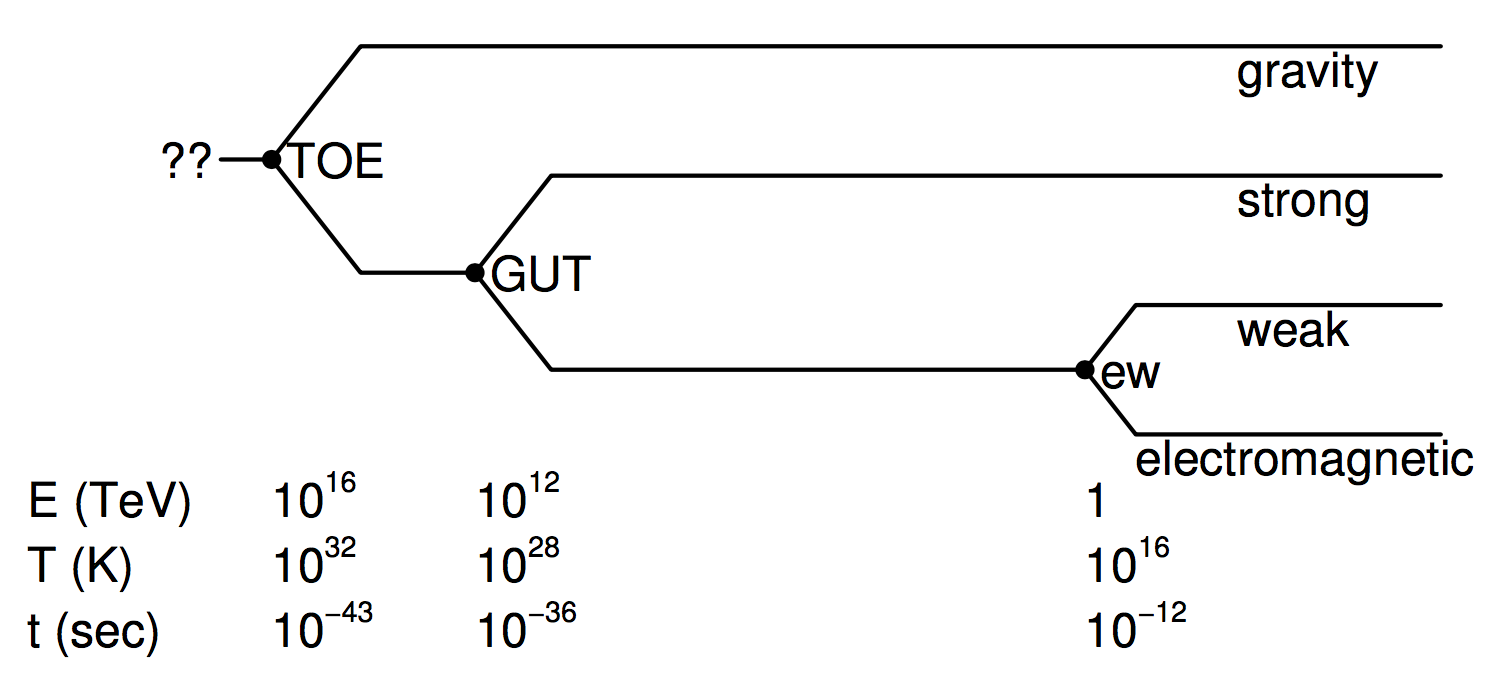
\includegraphics[width=16cm]{figures/cosmology/GUT.png}
    \centering
    \caption{\footnotesize{The energy, temperature, and time scales at which the different force unifications occur. Image taken from Ryden (2006).}}
    \label{fig:gut}
\end{figure}

{\noindent}One of the predictions of GUT is that the Universe underwent a phase transition as the temperature dropped below the GUT temperature. Generally speaking, phase transitions are associated with a spontaneous loss of symmetry as the temperature of a system is lowered. Take, as an example, the phase transition known as ``freezing water''. At temperatures $T>273\,{\rm K}$, water is liquid. Individual water molecules are randomly oriented, and the liquid water thus has rotational symmetry about any point; in other words, it is isotropic. However, when the temperature drops below $T=273\,{\rm K}$, the water undergoes a phase transition, from liquid to solid, and the rotational symmetry of the water is lost. The water molecules are locked into a crystalline structure, and the ice no longer has rotational symmetry about an arbitrary point. In other words, the ice crystal is anisotropic, with preferred directions corresponding to the crystal’s axes of symmetry. In a broadly similar vein, there is a loss of symmetry when the universe undergoes the GUT phase transition at $t_\mathrm{GUT}\sim10^{-36}\,{\rm s}$. At $T>T_\mathrm{GUT}$, there was a symmetry between the strong and electroweak forces. At $T<T_\mathrm{GUT}$, the symmetry is spontaneously lost; the strong and electroweak forces begin to behave quite differently from each other.

{\noindent}In general, phase transitions associated with a loss of symmetry give rise to flaws known as topological defects. To see how topological defects form, consider a large tub of water which is cooled below $T=273\,{\rm K}$. Usually, the freezing of the water will start at two or more widely separated nucleation sites. The crystal which forms about any given nucleation site is very regular, with well-defined axes of symmetry. However, the axes of symmetry of two adjacent ice crystals will be misaligned. At the boundary of two adjacent crystals, there will be a two-dimensional topological defect, called a domain wall, where the axes of symmetry fail to line up. Other types of phase transitions give rise to one-dimensional, or line-like, topological defects (in a cosmological context, these linear defects are known as cosmic strings). Still other types of phase transitions give rise to zero-dimensional, or point-like, topological defects. GUT predict that the GUT phase transition creates point-like topological defects which act as magnetic monopoles. That is, they act as the isolated north pole or south pole of a magnet. The rest energy of the magnetic monopoles created in the GUT phase transition is predicted to be $m_Mc^2\sim E_\mathrm{GUT}\sim10^{12}\,{\rm TeV}$. This corresponds to a mass of over a nanogram (comparable to that of a bacterium), which is a lot of mass for a single particle to be carrying around. At the time of the GUT phase transition, points further apart than the horizon size will be out of causal contact with each other. Thus, we expect roughly one topological defect per horizon volume, due to the mismatch of fields which are not causally linked. The number density of magnetic monopoles, at the time of their creation, would be

\begin{align*}
    n_M(t_\mathrm{GUT}) \sim \frac{1}{(2ct_\mathrm{GUT})^3} \sim 10^{82} ~ [{\rm m^{-3}}],
\end{align*}

{\noindent}and their energy density would be

\begin{align*}
    (m_Mc^2)n_M \sim 10^{94}\,{[\rm TeV\,m^{-3}]}.
\end{align*}

{\noindent}This is a large energy density, but it is smaller by ten orders of magnitude than the energy density of radiation at the time of the GUT phase transition:

\begin{align*}
    \alpha T_\mathrm{GUT}^4 \sim 10^{104}\,{[\rm TeV\,m^{-3}]}.
\end{align*}

{\noindent}Thus, the magnetic monopoles wouldn't have kept the Universe from being radiation-dominated at the time of the GUT phase transition. However, the magnetic monopoles, being so massive, would soon have become highly non-relativistic, with energy density $\propto a^{-3}$. The energy density in radiation, though, was falling off at the rate $\propto a^{-4}$. Thus, the magnetic monopoles would have dominated the energy density of the Universe when the scale factor had grown by a factor $\sim10^{10}$; that is, when the temperature had fallen to $T\sim10^{-10}\,T_\mathrm{GUT}\sim10^{18}\,{\rm K}$, and the age of the universe was only $t\sim10^{-16}\,{\rm s}$.

{\noindent}Obviously, the Universe is not dominated by magnetic monopoles today. In fact, there is no strong evidence that they exist at all. Every north magnetic pole which we can find is paired with a south magnetic pole, and vice versa. There are no isolated north poles or isolated south poles. The monopole problem can thus be rephrased as the question, ``Where have all the magnetic monopoles gone?'' Now, you can always answer the question, ``Where have the monopoles gone?'' by saying, ``There were never any monopoles to begin with''” There is not yet a single, definitive GUT, and in some variants on the GUT theme, magnetic monopoles are not produced. However, the flatness and horizon problems are not so readily dismissed. When the physicist Alan Guth first proposed the idea of inflation in 1981, he introduced it as a way of resolving the flatness problem, the horizon problem, and the monopole problem with a single cosmological mechanism.

\subsubsection{Follow-up Questions}

\begin{itemize}
    \item Can you calculate/give an estimate or back-of-the-envelope idea of how flat the universe would have been after inflation if today it was say 1\% non-flat?
    \item What physically causes inflation?
    \item Why, physically, does having an inflaton result in inflation? What physically happens?

\end{itemize}

% --------------------------------------------------------------
%
%                           12. 
%
% --------------------------------------------------------------

\newpage
\subsection{Question 12}

Define and describe a 'fine tuning problem'. How do anthropic arguments attempt to resolve it?

\subsubsection{Short answer}

Answer.

\subsubsection{Additional context}

Additional context.

\subsubsection{Follow-up Questions}

\begin{itemize}
    \item What are other fine tuning problems? (Note: if you talk about $\Omega_k$, you cannot talk about $\Omega_\Lambda$ since they are related.)
    \item How do you \textit{feel} about the anthropic principle?
\end{itemize}


% --------------------------------------------------------------
%
%                           13. 
%
% --------------------------------------------------------------

\newpage
\subsection{Question 13}

Define the two-point correlation function. How is it related to the power spectrum? How is the $C_\ell$ spectrum of the CMB related to low redshift galaxy clustering?

\subsubsection{Short answer}

Answer.

\subsubsection{Additional context}

Since the CMB temperature fluctuations $\delta T/T$ is defined on the surface of a sphere -- the celestial sphere, in this case -- it is useful to expand it in spherical harmonics:

\begin{align*}
    \frac{\delta T}{T}(\theta,\phi) = \sum\limits_{\ell=0}^{\infty}\sum\limits_{m=-1}^{\ell} a_{\ell m}Y_{\ell m}(\theta,\phi)
\end{align*}

{\noindent}where $Y_{\ell m}(\theta,\phi)$ are the usual spherical harmonic functions\footnote{\href{https://en.wikipedia.org/wiki/Table\_of\_spherical\_harmonics}{https://en.wikipedia.org/wiki/Table\_of\_spherical\_harmonics}}. What concerns cosmologists is not the exact pattern of hot spots and cold spots on the sky, but their statistical properties. The most important statistical property of $\delta T/T$ is the correlation function $C(\theta)$. Consider two points on the last scattering surface. Relative to an observer, they are in the directions $\hat{n}$ and $\hat{n}'$, and are separated by an angle $\theta$ given by the relation $cos\theta=\hat{n}\cdot\hat{n}'$. To find the correlation function $C(\theta)$, multiply together the values of $\delta T/T$ at the two points, then average the product over all points separated by the angle $\theta$:

\begin{align*}
    C(\theta) = \left\langle\frac{\delta T}{T}(\hat{n})\frac{\delta T}{T}(\hat{n}')\right\rangle_{\hat{n}\cdot\hat{n}'=\cos\theta}
\end{align*}

{\noindent}If cosmologists knew the precise value of $C(\theta)$ for all angles from $\theta=0$ to $\theta=180^\circ$, they would have a complete statistical description of the temperature fluctuations over all angular scales. Unfortunately, the CMB measurements which tell us about $C(\theta)$ contain information over only a limited range of angular scales.

{\noindent}The limited angular resolution of available observations is what makes the spherical harmonic expansion of $\delta T/T$ so useful. Using the expansion of $\delta T/T$ in spherical harmonics, the correlation function can be written in the form

\begin{align*}
    C(\theta) = \frac{1}{4\pi} \sum\limits_{\ell=0}^\infty (2\ell+\ell)(C_\ell)P_\ell(cos\theta),
\end{align*}

{\noindent}where $P_\ell$ are the usual Legendre polynomials:

\begin{align*}
    P_0(x) = 1 \\
    P_1(x) = x \\
    P_2(x) = \frac{1}{2}(3x^2-1)
\end{align*}

{\noindent}and so forth. In this way, a measured correlation function $C(\theta)$ can be broken down into its multipole moments $C_\ell$.

{\noindent}Generally speaking, a term $C_\ell$ is a measure of temperature fluctuations on the angular scale $\theta\sim180^\circ/\ell$. Thus, the multipole $\ell$ is interchangeable, for all practical purposes, with the angular scale $\theta$. The $\ell=0$ (monopole) term of the correlation function vanishes if you've defined the mean temperature correctly. The $\ell=1$ (dipole) term results primarily from the Doppler shift due to our motion through space. It is the moments with $\ell\geq2$ which are of the most interest to cosmologists, since they tell us about the fluctuations present at the time of last scattering.

{\noindent}In presenting the results of CMB observations, it is customary to plot the function

\begin{align*}
    \Delta T \equiv \sqrt{\frac{\ell(\ell+1)}{2\pi}}\langle T \rangle ~ [{\rm K}],
\end{align*}

{\noindent}since this function tells us the contribution per logarithmic interval in $\ell$ to the total temperature fluctuation $\delta T$ of the CMB. The detailed shape of the $\Delta T$ versus $\ell$ curve contains a wealth of information about the Universe at the time of photon decoupling. 

{\noindent}At the time of last scattering, a particularly interesting length scale, cosmologically speaking, is the Hubble distance,

\begin{align*}
    d_H = \frac{c}{H(z_\mathrm{ls})} \approx \frac{3\times10^8\,{\rm m\,s^{-1}}}{1.24\times10^{-18}\,s^{-1}(1101)^{3/2}} \approx 6.6\times10^{21}\,{\rm m} \approx 0.2\,{[\rm Mpc]},
\end{align*}

{\noindent}where the redshift of last scattering is $z_\mathrm{ls}\approx1100$. A patch of the last scattering surface with this physical size will have an angular size, as seen from Earth, of

\begin{align*}
    \theta_H = \frac{c/H(z_\mathrm{ls})}{d_A} \approx \frac{0.2\,{\rm Mpc}}{13\,{\rm Mpc}} \approx 0.015\,{\rm rad} \approx 1^\circ.
\end{align*}

{\noindent}It is no coincidence that the peak in the $\Delta T$ versus $\ell$ curve occurs at an angular scale $θ\sim\theta_H$. The origin of temperature fluctuations with $\theta>\theta_H$ ($\ell<180$) is different from those with $\theta<\theta_H$ ($\ell>180$).


% --------------------------------------------------------------
%
%                           14. 
%
% --------------------------------------------------------------

\newpage
\subsection{Question 14}

Consider a cosmological model including a positive cosmological constant. Show that, in such a model, the expansion factor eventually expands at an exponential rate. Sketch the time dependence of the expansion factor in the currently favoured cosmological model.

\subsubsection{Short answer}

Answer.

\subsubsection{Additional context}

The Benchmark Model, is adopted as the best fit to the currently available observational data, is spatially flat, and contains radiation, matter, and a cosmological constant. Some of its properties are listed, for ready reference, in Table 6.2. The Hubble constant of the Benchmark Model is assumed to be $H_0=70\,{\rm km\,s^{-1}\,Mpc^{-1}}$. The radiation in the Benchmark Model consists of photons and neutrinos. The photons are assumed to be provided solely by a CMB with current temperature $T_0=2.725\,{\rm K}$ and density parameter $\Omega_{\gamma,0}=5.0\times10^{-5}$. The energy density of the CNB is theoretically calculated to be 68\% of that of the CMB, as long as neutrinos are relativistic. If a neutrino has a non-zero mass $m_\nu$, it defects from the ``radiation'' column to the ``matter'' column when the scale factor is $a\sim5\times10^{-4}\,{\rm eV}/(m_\nu c^2)$. The matter content of the Benchmark Model consists partly of baryonic matter (that is, matter composed of protons and neutrons, with associated electrons), and partly of nonbaryonic dark matter; the evidence indicates that most of the matter in the Universe is nonbaryonic dark matter. The baryonic material that we are familiar with from our everyday existence has a density parameter of $\Omega_{b,0}\approx0.04$ today. The density parameter of the nonbaryonic dark matter is roughly six times greater: $\Omega_{c,0}\approx0.26$. The bulk of the energy density in the Benchmark Model, however, is not provided by radiation or matter, but by a cosmological constant, with $\Omega_{\Lambda,0}=1-\Omega_{m,0}-\Omega_{r,0}\approx0.70$.

{\noindent}The Benchmark Model was first radiation-dominated, then matter-dominated, and is now entering into its lambda-dominated phase. Radiation gave way to matter at a scale factor $a_{rm}=\Omega_{r,0}/\Omega{m,0}=2.8\times10^{-4}$, corresponding to a time $t_{rm}=4.7\times10^4\,{\rm yr}$. Matter, in turn, gave way to the cosmological constant at $a_{m\Lambda}=(\Omega_{m,0}/\Omega_{\Lambda,0})^{1/3}$ corresponding to $t_{m\Lambda}=9.8\,{\rm Gyr}$. The current age of the Universe, in the Benchmark Model, is $t_0=13.5\,{\rm Gyr}$.

{\noindent}With $\Omega_{r,0}$, $\Omega_{m,0}$, and $\Omega_{\Lambda,0}$ known, the scale factor $a(t)$ can be computed numerically using the Friedmann equation, in the form of

\begin{align*}
    \left(\frac{H}{H_0}\right)^2 = \frac{\Omega_{r,0}}{a^4} + \frac{\Omega_{m,0}}{a^3} + \Omega_{\Lambda,0} + \frac{1-\Omega_0}{a^2}
\end{align*}

{\noindent}where $\Omega_0=\Omega_{r,0}+\Omega_{m,0}+\Omega_{\Lambda,0}$. Since $(H/H_0)^2=(\dot{a}/a)^2$, this can be written as

\begin{align*}
    \left(\frac{\dot{a}(t)}{a(t)}\right)^2 &= \frac{\Omega_{r,0}}{a^4} + \frac{\Omega_{m,0}}{a^3} + \Omega_{\Lambda,0} + \frac{1-\Omega_0}{a^2} \\
    \dot{a}(t) &= a(t)\sqrt{\frac{\Omega_{r,0}}{a^4} + \frac{\Omega_{m,0}}{a^3} + \Omega_{\Lambda,0} + \frac{1-\Omega_0}{a^2}}.
\end{align*}

{\noindent}For $a\gg1$, this simplifies to

\begin{align*}
    \frac{\mathrm{d}a}{\mathrm{d}t} &\approx a(t)\sqrt{\Omega_{\Lambda,0}} \\
    a(t) &\approx e^{\sqrt{\Omega_{\Lambda,0}}t}.
\end{align*}

{\noindent}Therefore, at large scale factors, the expansion proceeds at the exponential rate as follows:

\begin{align*}
    a(t) \propto e^{\sqrt{\Omega_{\Lambda,0}}t}.
\end{align*}

{\noindent}Figure \ref{fig:avst} shows the scale factor, thus computed, for the Benchmark Model. Note that the transition from the $a\propto t^{1/2}$ radiation-dominated phase to the $a\propto t^{2/3}$ matter-dominated phase is not an abrupt one; neither is the later transition from the matter-dominated phase to the exponentially growing lambda-dominated phase. One curious feature of the Benchmark Model which Figure \ref{fig:avst} illustrates vividly is that we are living very close to the time of matter-lambda equality.

\begin{figure}[t]
    \floatbox[{\capbeside\thisfloatsetup{capbesideposition={right,top},capbesidewidth=4cm}}]{figure}[\FBwidth]
    {\caption{\footnotesize{The scale factor $a$ as a function of time $t$ (measured in units of the Hubble time), computed for the Benchmark Model. The dotted lines indicate the time of radiation-matter equality, $a_{rm}=2.8\times10^{-4}$, the time of matter-lambda equality, $a{m\Lambda}=0.75$, and the present moment, $a_0=1$. Figure taken from Ryden (2006).}}
    \label{fig:avst}}
    {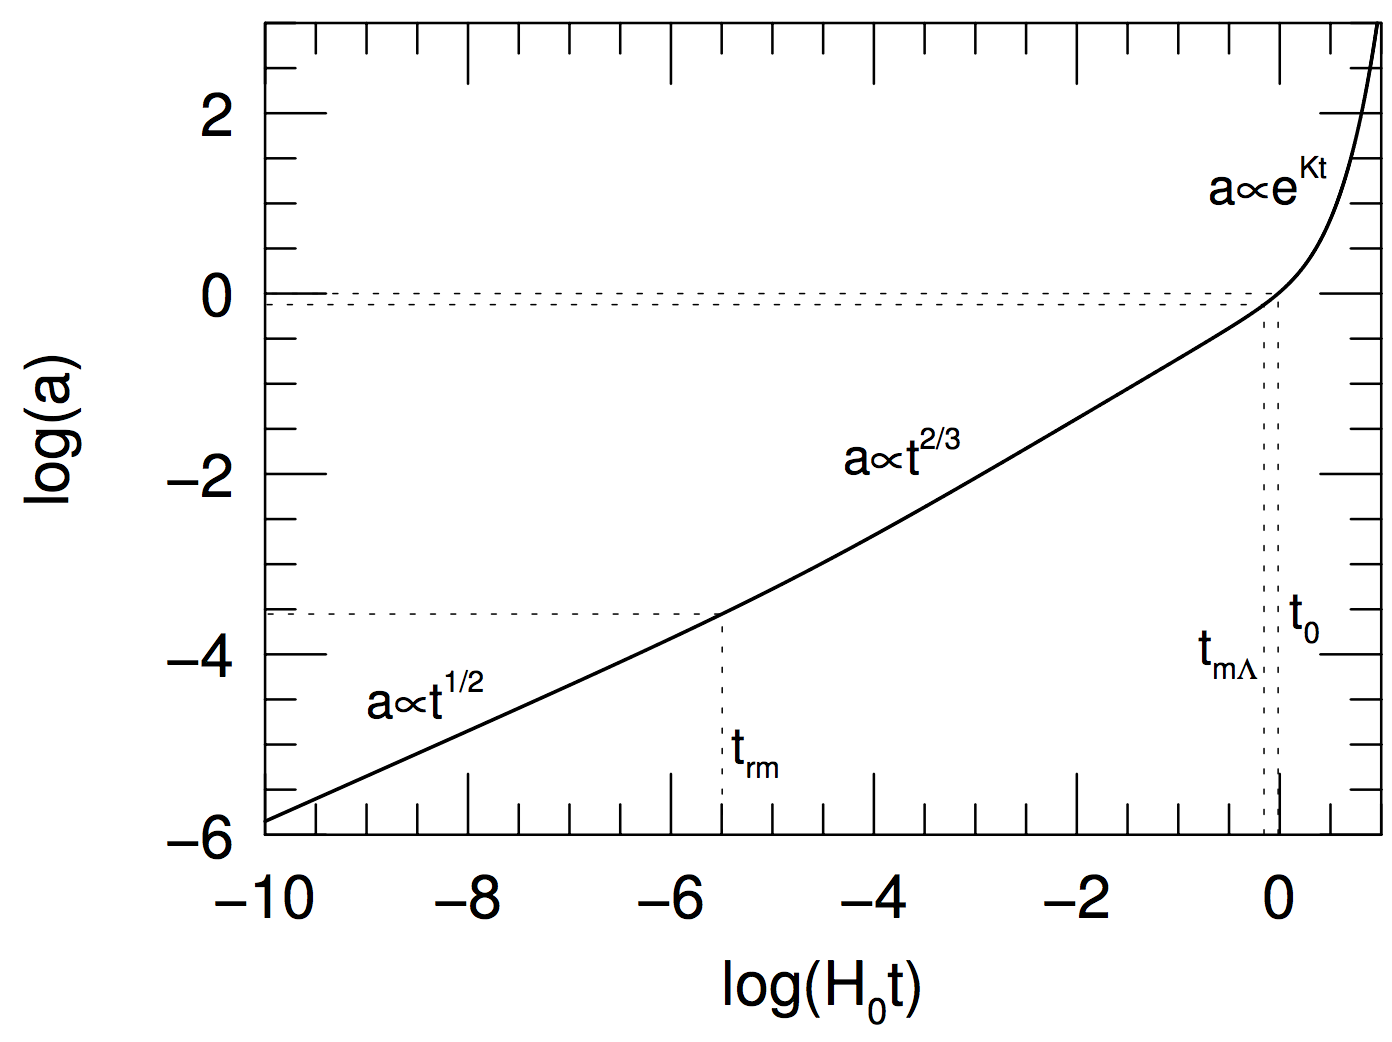
\includegraphics[width=12cm]{figures/cosmology/avst.png}}
\end{figure}

% --------------------------------------------------------------
%
%                           15. 
%
% --------------------------------------------------------------

\newpage
\subsection{Question 15}

Define and describe the epoch of reionization. What are the observational constraints on it?

\subsubsection{Short answer}

Answer.

\subsubsection{Additional context}

Additional context.

\subsubsection{Follow-up Questions}

\begin{itemize}
    \item Besides the first stars and galaxies, what else could have ionized the Universe?
    \item How does the recent paper by Bowman et al. relate to this?
\end{itemize}


% --------------------------------------------------------------
%
%                           16. 
%
% --------------------------------------------------------------

\newpage
\subsection{Question 16}

The $21\,{\rm cm}$ line of hydrogen is expected to show up in absorption against the cosmic microwave background at some redshifts, and in emission at other redshifts. What physical processes lead to this behaviour?

\subsubsection{Short answer}

Answer.

\subsubsection{Additional context}

Additional context.

% --------------------------------------------------------------
%
%                           17. 
%
% --------------------------------------------------------------

\newpage
\subsection{Question 17}

What is the difference between scalar and tensor modes of perturbation in the early universe, and how can you detect their presence?

\subsubsection{Short answer}

Short answer.

\subsubsection{Additional context}

{\noindent}Scalars, vectors, and tensors generate distinct patterns in the polarization of the CMB. However, although they separate cleanly into $m=0,\pm1,\pm2$ polarization patterns for a single plane wave perturbation in the coordinate system referenced to $k\bm{k}$, in general there will exist a spectrum of fluctuations each with a different $\bm{k}$. Therefore the polarization pattern on the sky does not separate into $m=0,\pm1,\pm2$ modes. In fact, assuming statistical isotropy, one expects the ensemble averaged power for each multipole $\ell$ to be independent of $m$. Nonetheless, certain properties of the polarization patterns do survive superposition of the perturbations: in particular, its parity and its correlation with the temperature fluctuations.

\begin{figure}[h]
    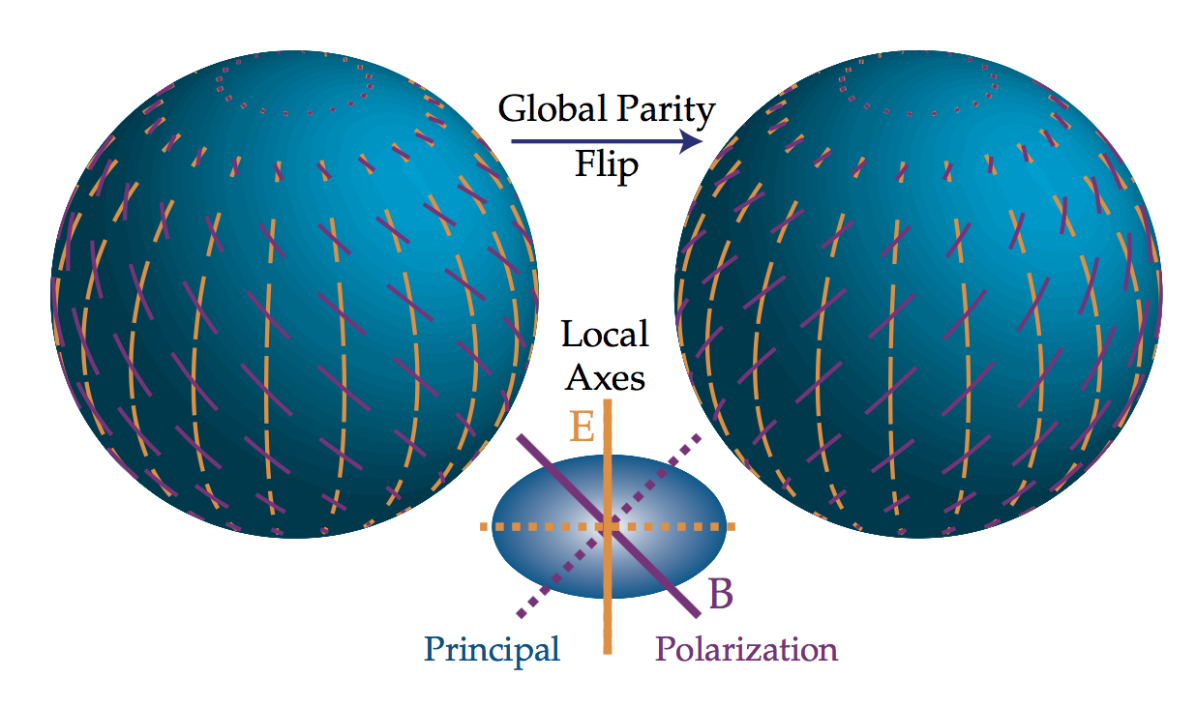
\includegraphics[width=16cm]{figures/cosmology/EBmodes.png}
    \centering
    \caption{\footnotesize{The electric ($E$) and magnetic ($B$) modes are distinguished by their behavior under a parity transformation $\bm{\hat{n}}\rightarrow\bm{\hat{n}}$. $E$-modes have $(-1)^\ell$ and $B$-modes have $(-1)^{\ell+1}$ parity; here ($\ell=2,m=0$), even and odd respectively. The local distinction between the two is that the polarization axis is aligned with the principle axes of the polarization amplitude for $E$ and crossed with them for $B$. Dotted lines represent a sign reversal in the polarization. Image taken from Hu \& White (1997).}}
    \label{fig:ebmodes}
\end{figure}

{\noindent}\textbf{Scalar (compressible) perturbations}:

{\noindent}The most commonly considered and familiar types of perturbations are scalar modes. These modes represent perturbations in the (energy) density of the cosmological fluid(s) at last scattering and are the only fluctuations which can form structure though gravitational instability. Consider a single large-scale Fourier component of the fluctuation (i.e., for the photons, a single plane wave in the temperature perturbation). Over time, the temperature and gravitational potential gradients cause a bulk flow, or dipole anisotropy, of the photons. Both effects can be described by introducing an “effective” temperature

\begin{align*}
    \left(\frac{\Delta T}{T}\right)_\mathrm{eff} = \left(\frac{\Delta T}{T}\right) + \psi,
\end{align*}

{\noindent}where $\psi$ is the gravitational potential. Gradients in the effective temperature always create flows from hot to cold effective temperature. Formally, both pressure and gravity act as sources of the momentum density of the fluid in a combination that is exactly the effective temperature for a relativistic fluid.

{\noindent} To avoid confusion, let us explicitly consider the case of adiabatic fluctuations, where initial perturbations to the density imply potential fluctuations that dominate at large scales. Here gravity overwhelms pressure in overdense regions causing matter to flow towards density peaks initially. Nonetheless, overdense regions are effectively cold initially because photons must climb out of the potential wells they create and hence lose energy in the process. Though flows are established from cold to hot temperature regions on large scales, they still go from hot to cold effective temperature regions. This property is true more generally of our adiabatic assumption: we hereafter refer only to effective temperatures to keep the argument general.

\begin{figure}[t!]
    \centering
    \vspace{-1cm}
    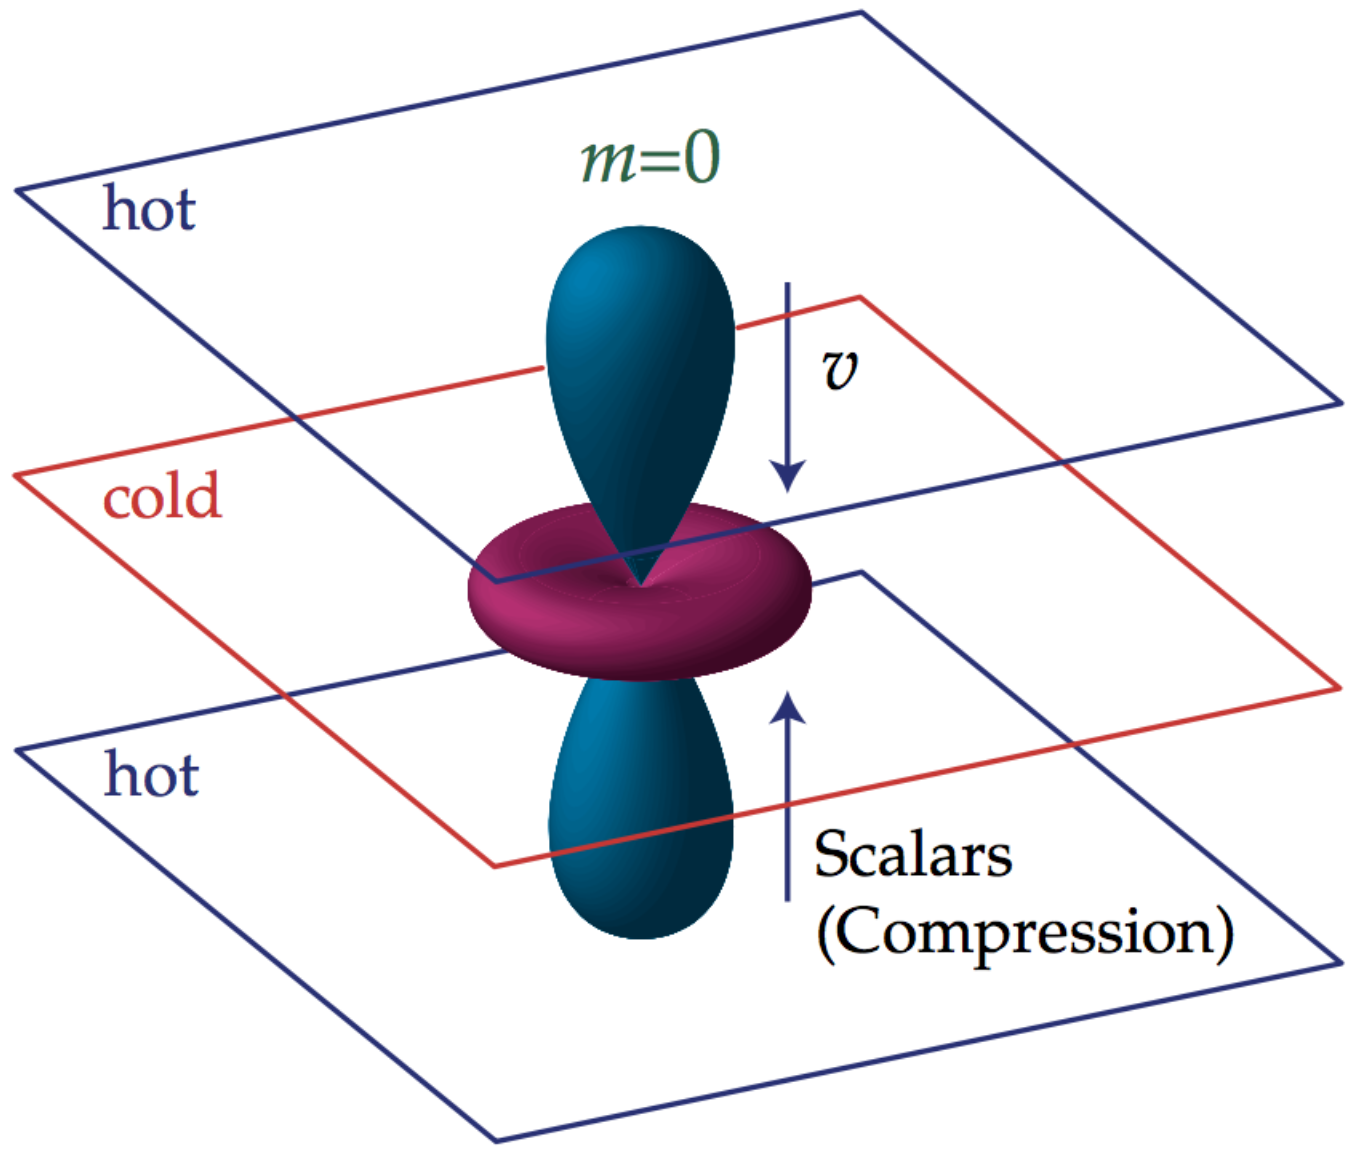
\includegraphics[width=8cm]{figures/cosmology/ScalarQuadrupole.png}\\
    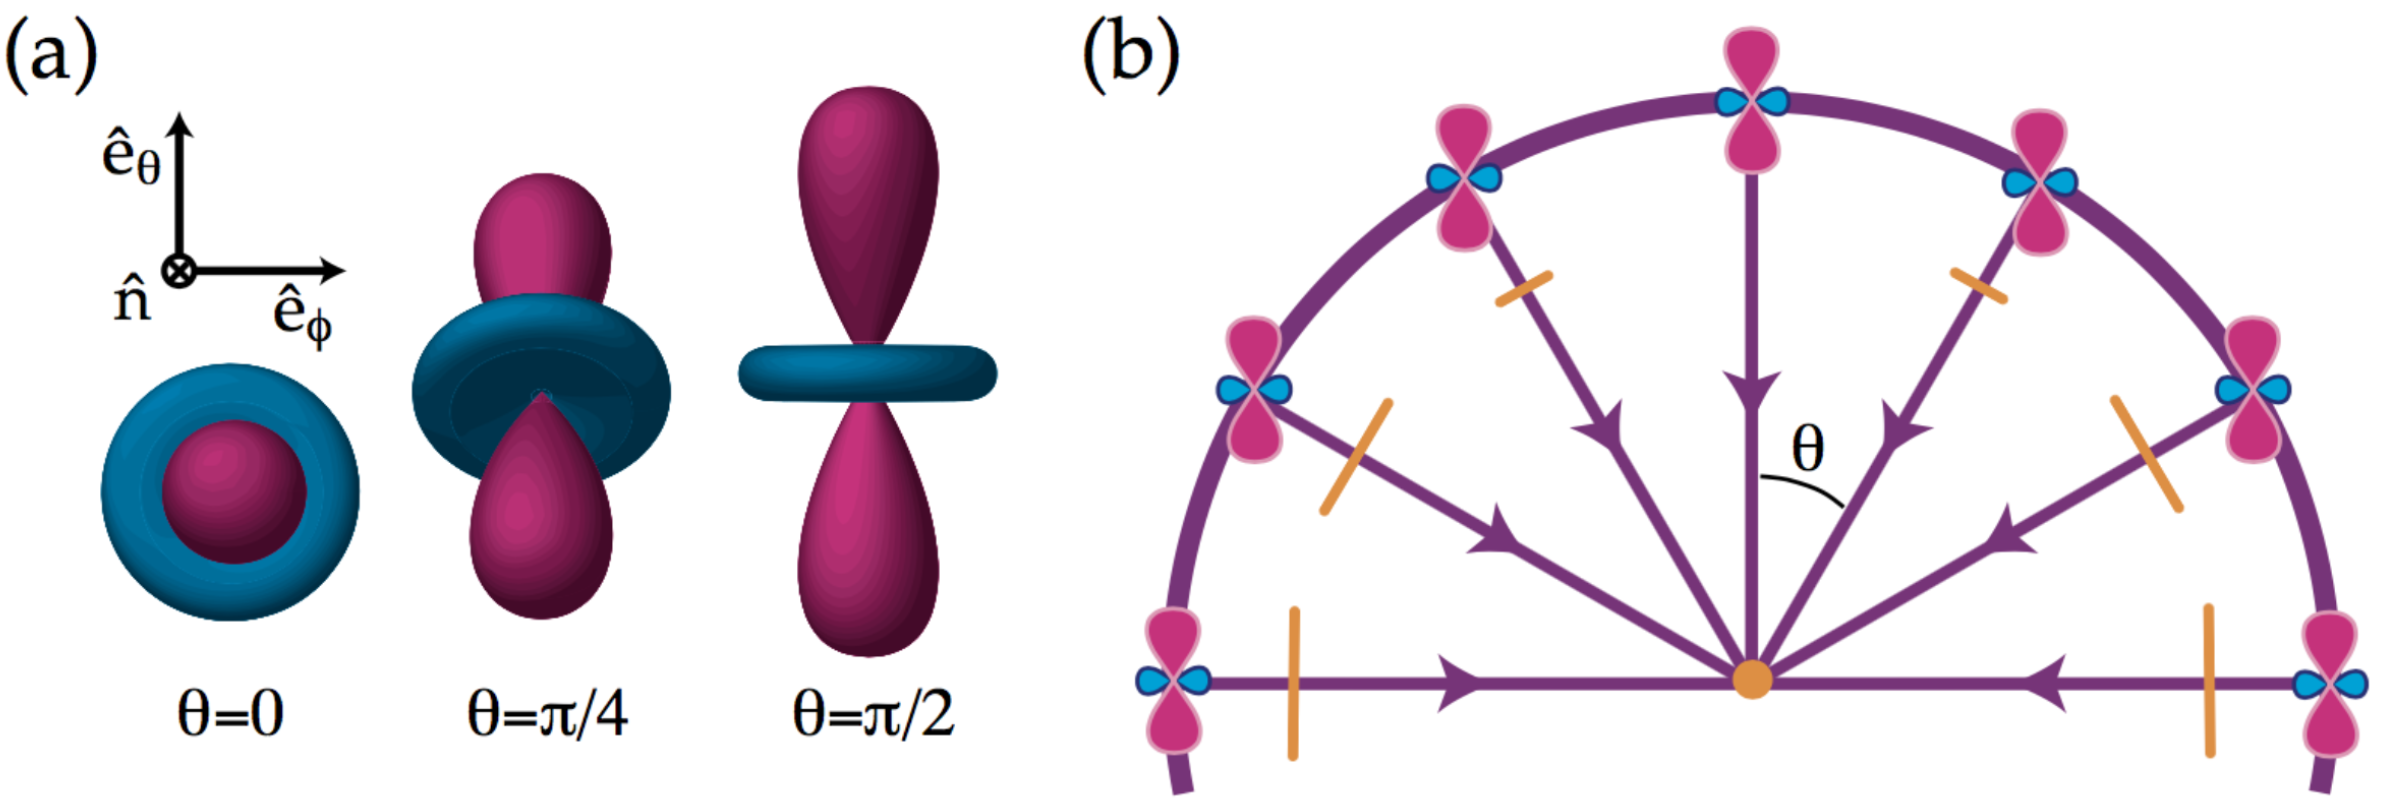
\includegraphics[width=15cm]{figures/cosmology/QuadrupolarAnisotropies.png}\\
    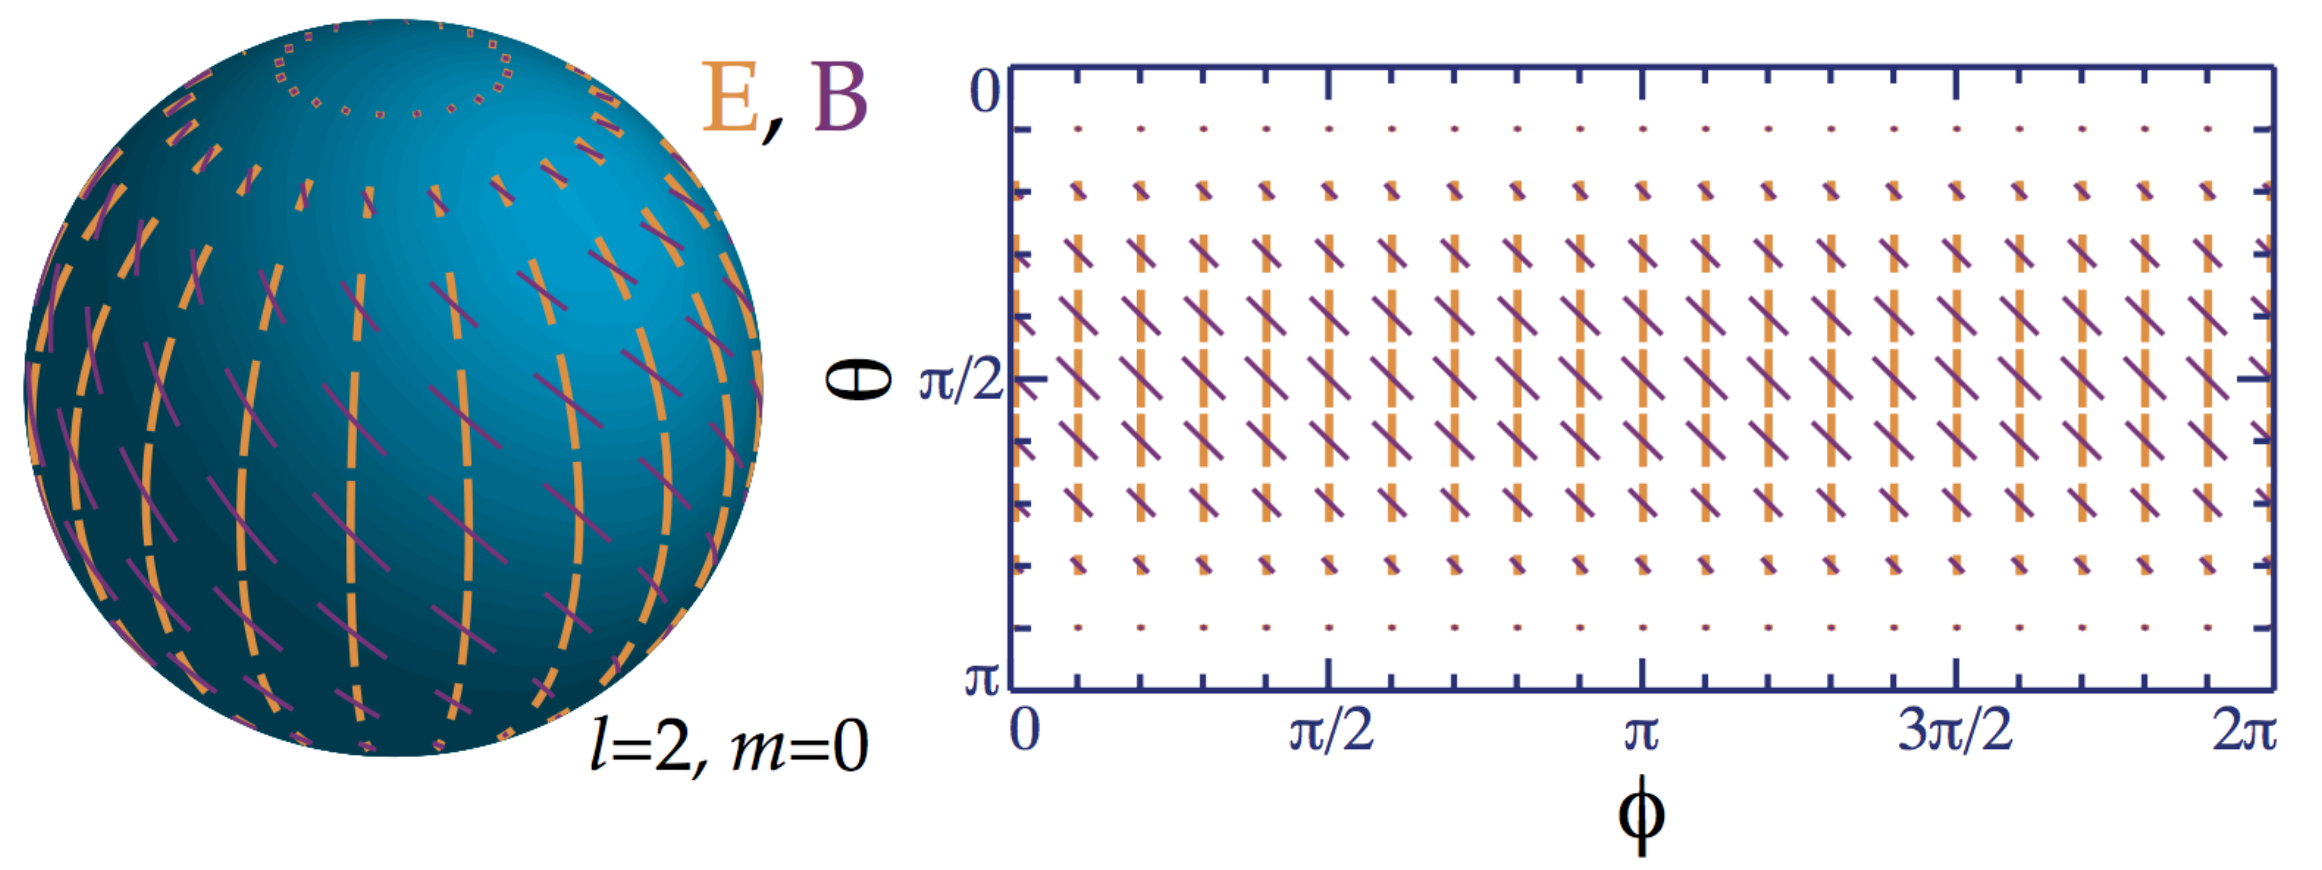
\includegraphics[width=15cm]{figures/cosmology/ScalarPattern.png}
    \caption{\footnotesize{\textbf{(Top)} The scalar quadrupole moment ($\ell=2,m=0$). Flows from hot (blue) regions into cold (red), $\bm{v}\parallel\bm{k}$, produce the azimuthally symmetric pattern $Y_2^0$ depicted here. \textbf{(Middle)} The transformation of quadrupole anisotropies into linear polarization. (a) The orientation of the quadrupole moment with respect to the scattering direction $\bm{\hat{n}}$ determines the sense and magnitude of the polarization. It is aligned with the cold (red, long) lobe in the $\bm{\hat{e}}_\theta\times\bm{\hat{e}}_\phi$ tangent plane. (b) In spherical coordinates where $\bm{\hat{n}}\cdot\bm{\hat{k}}=\cos\theta$, the polarization points north-south ($Q$) with magnitude varying as $\sin^2θ$ for scalar fluctuations. \textbf{(Bottom)} Polarization pattern for $\ell=2,m=0$, note the azimuthal symmetry. The scattering of a scalar $m=0$ quadrupole perturbation generates the electric $E$ (yellow, thick lines) pattern on the sphere. Its rotation by $45^\circ$ represents the orthogonal magnetic $B$ (purple, thin lines) pattern. Animation (available at \href{http://www.sns.ias.edu/∼whu/polar/scalaran.html}{http://www.sns.ias.edu/∼whu/polar/scalaran.html}): as the line of sight $\bm{\hat{n}}$ changes, the lobes of the quadrupole rotate in and out of the tangent plane. The polarization follows the orientation of the colder (red) lobe in the tangent plane. Images taken from Hu \& White (1997).}}
    \label{fig:scalar}
\end{figure}

{\noindent}Let us consider the quadrupole component of the temperature pattern seen by an observer located in a trough of a plane wave. The azimuthal symmetry in the problem requires that $\bm{v}\parallel\bm{k}$ and hence the flow is irrotational $\nabla\times\bm{v}=0$. Because hotter photons from the crests flow into the trough from the $\pm k$ directions while cold photons surround the observer in the plane, the quadrupole pattern seen in a trough has an $m = 0$,

\begin{align*}
    Y_2^0 \propto 3\cos^2\theta-1,
\end{align*}

{\noindent}structure with angle $\bm{\hat{n}\cdot\hat{k}}=\cos\theta$ (see top of Figure \ref{fig:scalar}). The opposite effect occurs at the crests, reversing the sign of the quadrupole but preserving the $m=0$ nature in its local angular dependence. The full effect is thus described by a local quadrupole modulated by a plane wave in space, $-Y_2^0(\bm{\hat{n}})\exp(i\bm{k}\cdot\bm{x})$, where the sign denotes the fact that photons flowing into cold regions are hot. This infall picture must be modified slightly on scales smaller than the sound horizon where pressure plays a role, however the essential property that the flows are parallel to $\bm{\hat{k}}$ and thus generate an $m=0$ quadrupole remains true.

{\noindent}The sense of the quadrupole moment determines the polarization pattern through Thomson scattering. Recall that polarized scattering peaks when the temperature varies in the direction orthogonal to $\bm{\hat{n}}$. Consider then the tangent plane $\bm{\hat{e}}_\theta\times\bm{\hat{e}}_\phi$ with normal $\bm{\hat{n}}$. This may be visualized in an angular ``lobe'' diagram such as the top of Figure \ref{fig:scalar} as a plane which passes through the ``origin'' of the quadrupole pattern perpendicular to the line of sight. The polarization is maximal when the hot and cold lobes of the quadrupole are in this tangent plane, and is aligned with the component of the colder lobe which lies in the plane. As $\theta$ varies from $0$ to $\pi/2$ (pole to equator) the temperature differences in this plane increase from zero (see middle of Figure \ref{fig:scalar} a). The local polarization at the crest of the temperature perturbation is thus purely in the N-S direction tapering off in amplitude toward the poles (see middle of Figure \ref{fig:scalar} b). This pattern represents a pure $Q$-field on the sky whose amplitude varies in angle as an $\ell=2,m=0$ tensor or spin-$2$ spherical harmonic (Newman \& Penrose, 1966)

\begin{align*}
    Q=\sin^2\theta,~~~~~U=0.
\end{align*}

{\noindent}In different regions of space, the plane wave modulation of the quadrupole can change the sign of the polarization, but not its sense.

{\noindent}This pattern (bottom of Figure \ref{fig:scalar}, thick lines) is of course not the only logical possibility for an $\ell=2,m=0$ polarization pattern. Its rotation by $45^\circ$ is also a valid configuration (thin lines). This represents a pure NW-SE (and by sign reversal NE-SW), or $U$-polarization pattern (a distinction between the two patterns being electric and magnetic modes).

{\noindent}\textbf{Vector (vortical) perturbations}:

{\noindent}Vector perturbations represent vortical motions of the matter, where the velocity field $\bm{v}$ obeys $\nabla\cdot\bm{v}=0$ and $\nabla\times\bm{v}\neq0$, similar to ``eddies'' in water. There is no associated density perturbation, and the vorticity is damped by the expansion of the Universe as are all motions that are not enhanced by gravity. However, the associated temperature fluctuations, once generated, do not decay as both $\Delta T$ and $T$ scale similarly with the expansion. For a plane wave perturbation, the velocity field $\bm{v}\perp\bm{k}$ with direction reversing in crests and troughs (see top of Figure \ref{fig:vector}). The radiation field at these extrema possesses a dipole pattern due to the Doppler shift from the bulk motion. Quadrupole variations vanish here but peak between velocity extrema. To see this, imagine sitting between crests and troughs. Looking up toward the trough, one sees the dipole pattern projected as a hot and cold spot across the zenith; looking down toward the crest, one sees the projected dipole reversed. The net effect is a quadrupole pattern in temperature with $m\pm1$

\begin{align*}
    Y_2^{\pm1}\propto\sin\theta\cos\theta\mathrm{e}{\pm i\phi}.
\end{align*}

\begin{figure}[t!]
    \centering
    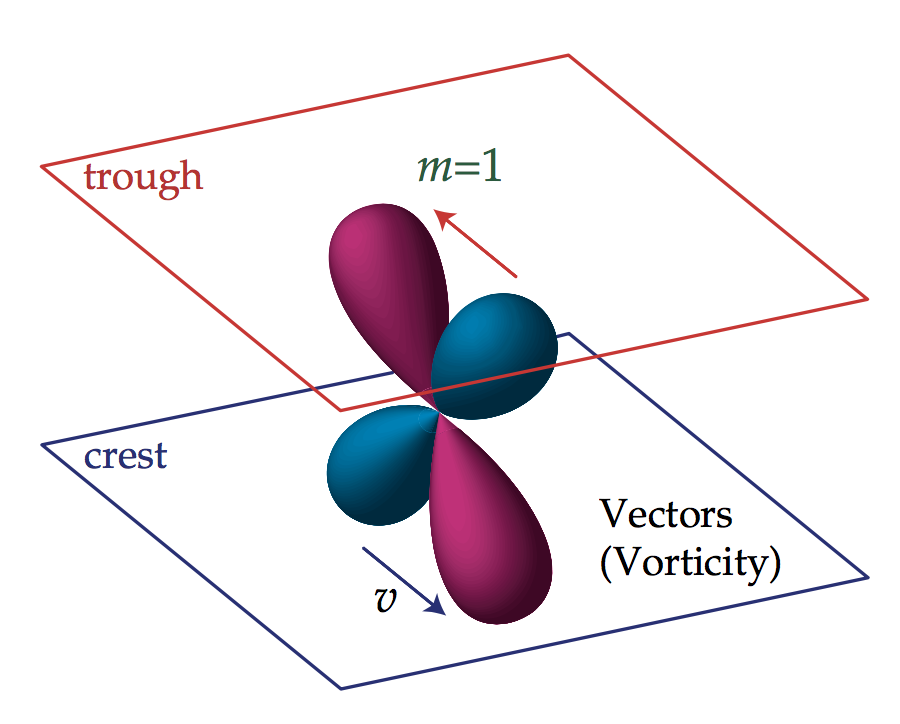
\includegraphics[width=8cm]{figures/cosmology/VectorQuadrupole.png}
    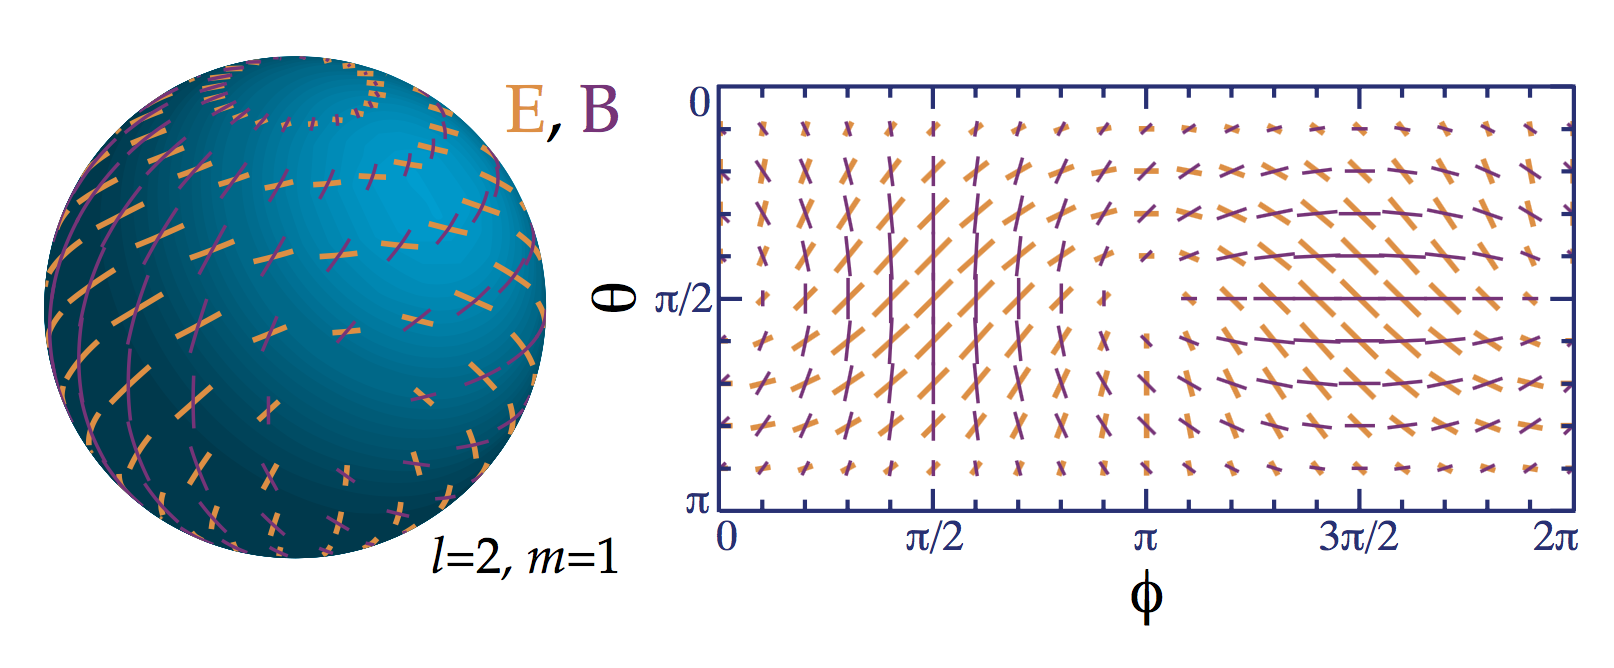
\includegraphics[width=15cm]{figures/cosmology/VectorPattern.png}
    \caption{\footnotesize{\textbf{(Top)} The vector quadrupole moment ($l=2,m=1$). Since $\bm{v}\perp\bm{k}$, the Doppler effect generates a quadrupole pattern with lobes $45^\circ$ from $\bm{v}$ and $\bm{k}$ that is spatially out of phase (interplane peaks) with $v$. \textbf{(Bottom)} Polarization pattern for $\ell=2,m=1$. The scattering of a vector ($m=1$) quadrupole perturbation generates the $E$ pattern (yellow, thick lines) as opposed to the $B$, (purple, thin lines) pattern. Animation (available at \href{http://www.sns.ias.edu/∼whu/polar/vectoran.html}{http://www.sns.ias.edu/∼whu/polar/vectoran.html}): same as for scalars. Images taken from Hu \& White (1997).}}
    \label{fig:vector}
\end{figure}

{\noindent}The lobes are oriented at $45^\circ$ from $k$ and $v$ since the line
of sight velocity vanishes along $k$ and at $90$ degrees to $k$ here. The latter follows since midway between the crests and troughs $v$ itself is zero. The full quadrupole distribution is therefore described by $-iY_2^{\pm1}(\bm{\hat{n}})\exp(i\bm{k}\cdot\bm{x})$, where $i$ represents the spatial phase shift of the quadrupole with respect to the velocity.

{\noindent}Thomson scattering transforms the quadrupole temperature anisotropy into a local polarization field as before. Again, the pattern may be visualized from the intersection of the tangent plane to $\bm{\hat{n}}$ with the lobe pattern of the top of Figure \ref{fig:vector}. At the equator ($\theta=\pi/2$), the lobes are oriented $45^\circ$ from the line of sight $\bm{\hat{n}}$ and rotate into and out of the tangent plane with $\phi$. The polarization pattern here is a pure $U$-field which varies in magnitude as $\sin\phi$. At the pole $\theta=0$, there are no temperature variations in the tangent plane so the polarization vanishes. Other angles can equally well be visualized by viewing the quadrupole pattern at different orientations given by $\bm{\hat{n}}$.

{\noindent}The full $\ell=2,m=1$ pattern,

\begin{align*}
    Q=-\sin\theta\cos\theta\mathrm{e}^{i\phi},~~~~~U=-i\sin\theta\mathrm{e}^{i\phi}
\end{align*}

{\noindent}is displayed explicitly in the bottom of Figure \ref{fig:vector}. Note that the pattern is dominated by $U$-contributions especially near the equator.

{\noindent}\textbf{Tensor (gravitational wave) perturbations}:

{\noindent}Tensor fluctuations are transverse-traceless perturbations to the metric, which can be viewed as gravitational waves. A plane gravitational wave perturbation represents a quadrupolar ``stretching'' of space in the plane of the perturbation (see Figure \ref{fig:tensorquadrupole}). As the wave passes or its amplitude changes, a circle of test particles in the plane is distorted into an ellipse whose semi-major axis $\rightarrow$ semi-minor axis as the spatial phase changes from crest $\rightarrow$ trough (see the top of Figure \ref{fig:tensor}, yellow ellipses). Heuristically, the accompanying stretching of the wavelength of photons produces a quadrupolar temperature variation with an $m=\pm2$ pattern

\begin{align*}
    Y_2^{\pm2}\propto\sin^2\theta\mathrm{e}^{\pm2i\phi}
\end{align*}

{\noindent}in the coordinates defined by $\bm{\hat{k}}$.

\begin{figure}[t!]
    \centering
    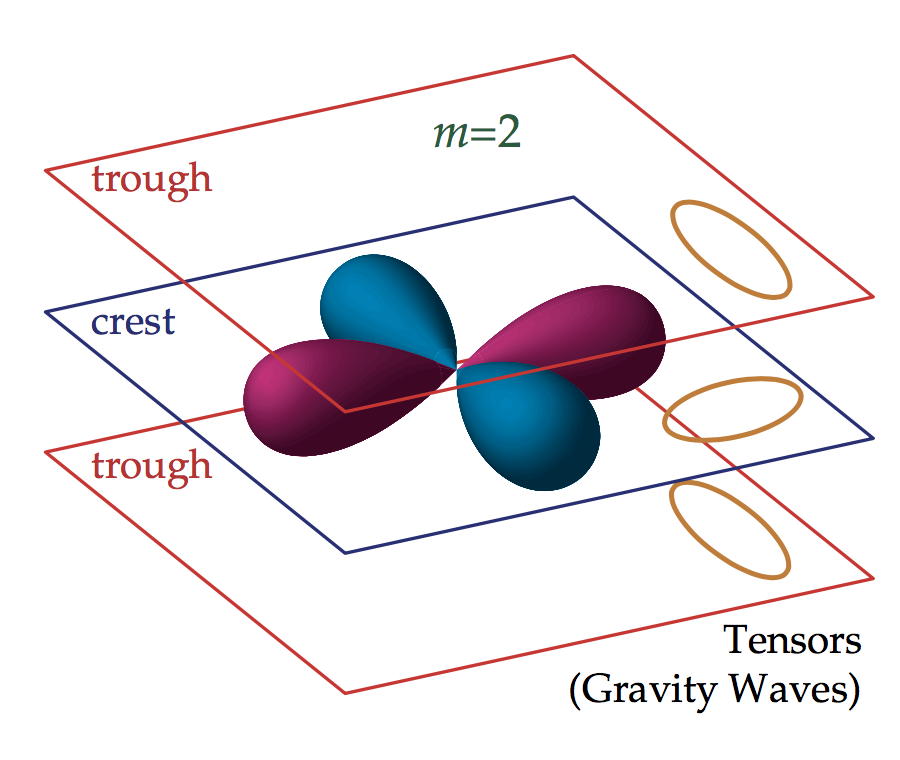
\includegraphics[width=8cm]{figures/cosmology/TensorQuadrupole.png}
    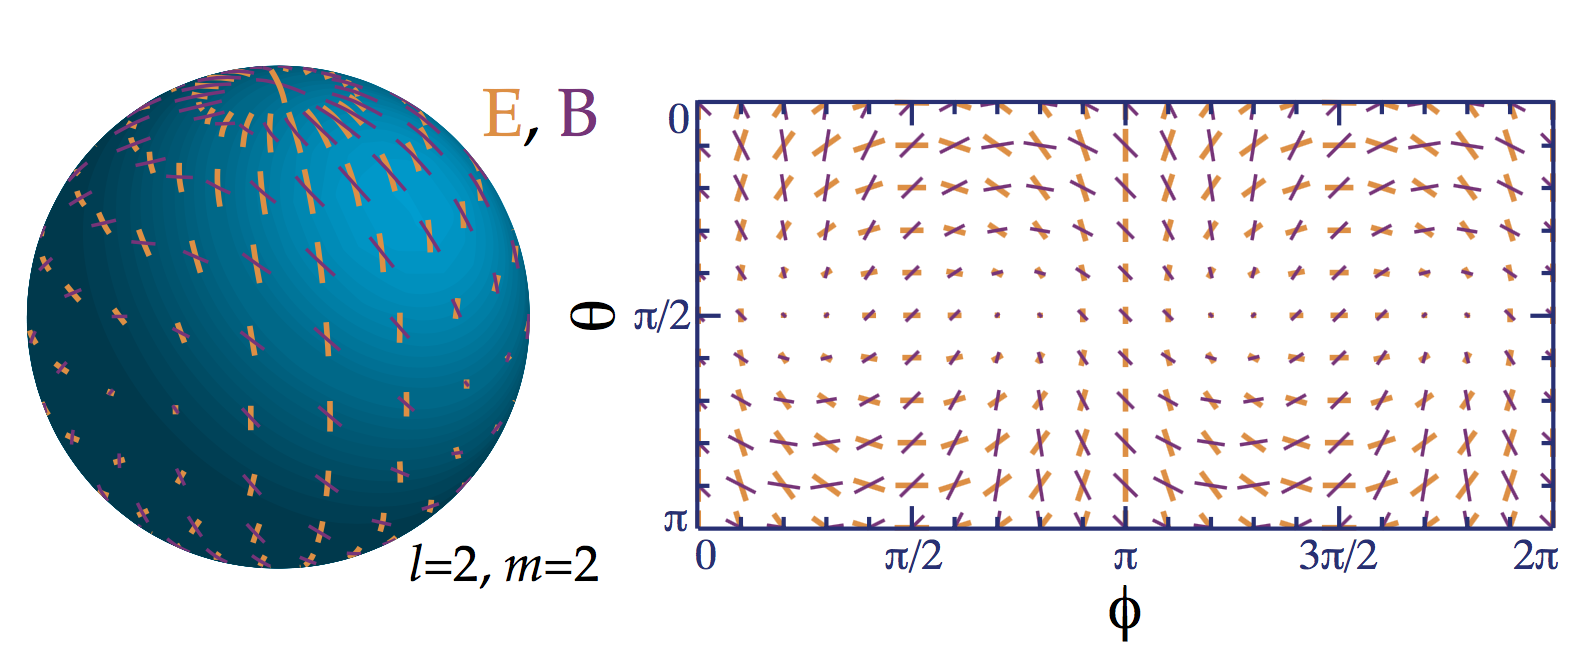
\includegraphics[width=15cm]{figures/cosmology/TensorPattern.png}
    \caption{\footnotesize{\textbf{(Top)} The tensor quadrupole moment $(m=2)$. Since gravity waves distort space in the plane of the perturbation, changing a circle of test particles into an ellipse, the radiation acquires an $m=2$ quadrupole moment. \textbf{(Bottom)} Polarization pattern for $\ell=2,m=2$. Scattering of a tensor $m=2$ perturbation generates the $E$ (yellow, thick lines) pattern as opposed to the $B$ (purple, thin lines) pattern. Animation (available at \href{http://www.sns.ias.edu/∼whu/polar/vectoran.html}{http://www.sns.ias.edu/∼whu/polar/vectoran.html}): same as for scalars. Images taken from Hu \& White (1997).}}
    \label{fig:tensor}
\end{figure}

{\noindent}Thomson scattering again produces a polarization pattern from the quadrupole anisotropy. At the equator, the quadrupole pattern intersects the tangent ($\bm{\hat{e}}_\theta\times\bm{\hat{e}}_\phi$) plane with hot and cold lobes rotating in and out of the $\bm{\hat{e}}_\phi$ direction with the azimuthal angle $\phi$. The polarization pattern is therefore purely $Q$ with a $\cos(2\phi)$ dependence. At the pole, the quadrupole lobes lie completely in the polarization plane and produces the maximal polarization unlike the scalar and vector cases. The full pattern,

\begin{align*}
    Q=(1+\cos^2\theta)\mathrm{e}^{2i\phi}~[{\rm Jy}], ~~~~~U=-2i\cos\theta\mathrm{e}^{2i\phi}~[{\rm Jy}],
\end{align*}

{\noindent}is shown in the bottom of Figure \ref{fig:tensor} (real part). Note that $Q$ and $U$ are present in nearly equal amounts for the tensors.

{\noindent}\textit{Electric and Magnetic Modes}:

{\noindent}Any polarization pattern on the sky can be separated into ``electric'' ($E$) and ``magnetic'' ($B$) components. This decomposition is useful both observationally and theoretically. There are two equivalent ways of viewing the modes that reflect their global and local properties respectively. The nomenclature reflects the global property. Like multipole radiation, the harmonics of an $E$-mode have $(-1)^\ell$ parity on the sphere, whereas those of a $B$-mode have $(-1)^{\ell+1}$ parity. Under $\bm{\hat{n}}\rightarrow\bm{\hat{n}}$, the $E$-mode thus remains unchanged for even $\ell$, whereas the $B$-mode changes sign as illustrated for the simplest case $\ell=2,m=0$ in Figure \ref{fig:ebmodes} (recall that a rotation by $90^\circ$ represents a change in sign). Note that the $E$ and $B$ multipole patterns are $45^\circ$ rotations of each other, (i.e. $Q\rightarrow U$ and $U\rightarrow-Q$). Since this parity property is obviously rotationally invariant, it will survive integration over $\bm{\hat{k}}$.

{\noindent}The local view of $E$- and $B$-modes involves the second derivatives of the polarization amplitude (second derivatives because polarization is a tensor or spin-$2$ object). In much the same way that the distinction between electric and magnetic fields in electromagnetism involves vanishing of gradients or curls (i.e., first derivatives) for the polarization there are conditions on the second (covariant) derivatives of $Q$ and $U$. For an $E$-mode, the difference in second (covariant) derivatives of $U$ along $\bm{\hat{e}}_\theta$ and $\bm{\hat{e}}_\phi$ vanishes as does that for $Q$ along $\bm{\hat{e}}_\theta+\bm{\hat{e}}_\phi$ and $\bm{\hat{e}}_\theta-\bm{\hat{e}}_\phi$. For a $B$-mode, $Q$ and $U$ are interchanged. Recalling that a $Q$-field points in the $\bm{\hat{e}}_\theta$ or $\bm{\hat{e}}_\phi$ direction and a $U$-field in the crossed direction, we see that the Hessian or curvature matrix of the polarization amplitude has principle axes in the same sense as the polarization for $E$ and $45^\circ$ crossed with it for $B$ (see Figure \ref{fig:ebmodes}). Stated another way, near a maximum of the polarization (where the first derivative vanishes) the direction of greatest change in the polarization is parallel/perpendicular and at $45^\circ$ degrees to the polarization in the two cases.

{\noindent}The distinction is best illustrated with examples. Take the simplest case of $\ell=2,m=0$ where the $E$-mode is a $Q=\sin^2\theta$ field and the $B$-mode is a $U=\sin^2\theta$ field (see the bottom of Figure \ref{fig:scalar}). In both cases, the major axis of the curvature lies in the $\bm{\hat{e}}_\theta$ direction. For the $E$-mode, this is in the same sense; for the $B$-mode it is crossed with the polarization direction. The same holds true for the $m=1,2$ modes as can be seen by inspection of the bottom of Figure \ref{fig:vector} and the bottom of Figure \ref{fig:tensor}.

\begin{figure}[t!]
    \centering
    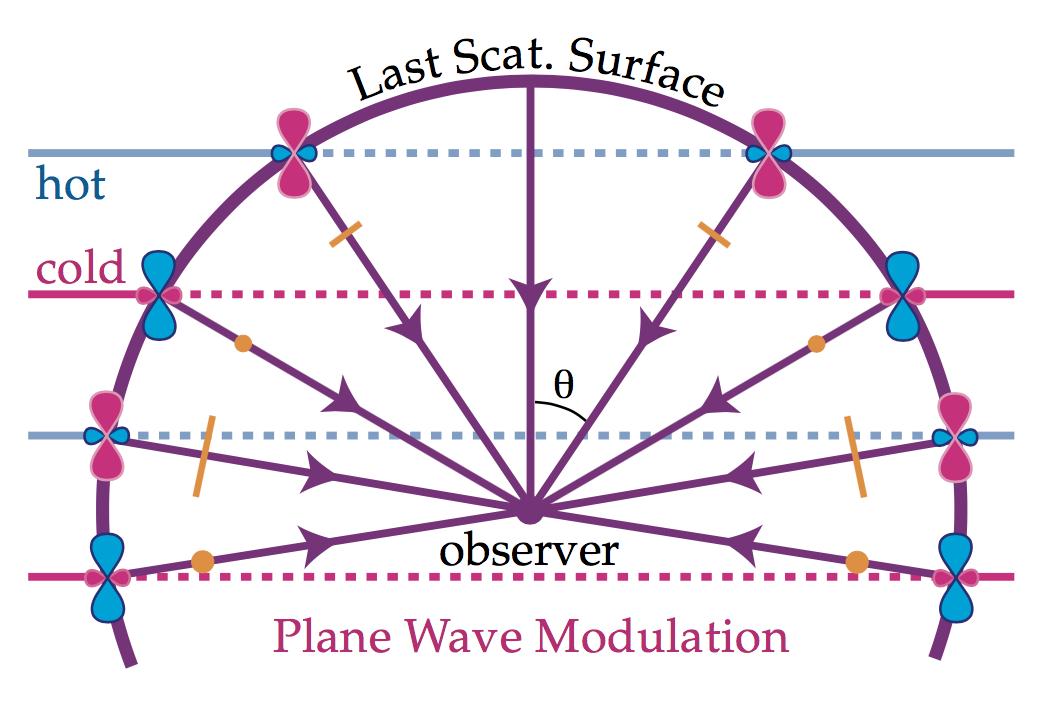
\includegraphics[width=10cm]{figures/cosmology/CMBquad.png}
    \caption{\footnotesize{Modulation of the local pattern in the bottom of Figure \ref{fig:scalar} by plane wave fluctuations on the last scattering surface. Yellow points represent polarization out of the plane with magnitude proportional to sign. The plane wave modulation changes the amplitude and sign of the polarization but does not mix $Q$ and $U$. Modulation can mix $E$ and $B$ however if $U$ is also present. Image taken from Hu \& White (1997).}}
    \label{fig:cmbquad}
\end{figure}

{\noindent}Thomson scattering can only produce an $E$-mode locally since the spherical harmonics that describe the temperature anisotropy have $(-1)^\ell$ electric parity. In the tops of Figures \ref{fig:scalar}, \ref{fig:vector}, and \ref{fig:tensor}, the $\ell=2,m=0,1,2$ $E$-mode patterns are shown in yellow. The $B$-mode represents these patterns rotated by $45^\circ$ and are shown in purple and cannot be generated by scattering. In this way, the scalars, vectors, and tensors are similar in that scattering produces a local $\ell=2$ $E$-mode only.

{\noindent}However, the pattern of polarization on the sky is not simply this local signature from scattering but is modulated over the last scattering surface by the plane wave spatial dependence of the perturbation (compare the bottom of Figure \ref{fig:scalar} and \ref{fig:cmbquad}). The modulation changes the amplitude, sign, and angular structure of the polarization but not its nature, e.g. a $Q$-polarization remains Q. Nonetheless, this modulation generates a $B$-mode from the local $E$-mode pattern.

{\noindent}The reason why this occurs is best seen from the local distinction between $E$ and $B$-modes. Recall that $E$-modes have polarization amplitudes that change parallel or perpendicular to, and $B$-modes in directions $45^\circ$ away from, the polarization direction. On the other hand, plane wave modulation always changes the polarization amplitude in the direction $\bm{\hat{k}}$ or N-S on the sphere. Whether the resultant pattern possesses $E$ or $B$-contributions depends on whether the local polarization has $Q$ or $U$-contributions.

{\noindent}For scalars, the modulation is of a pure $Q$-field and thus its $E$-mode nature is preserved (Kamionkowski et al. 1997; Zaldarriaga \& Seljak 1997). For the vectors, the $U$-mode dominates the pattern and the modulation is crossed with the polarization direction. Thus vectors generate mainly $B$-modes for short wavelength fluctuations (Hu \& White 1997). For the tensors, the comparable $Q$ and $U$ components of the local pattern imply a more comparable distribution of $E$ and $B$ modes at short wavelengths (see Figure \ref{fig:polpatterns}a).

\begin{figure}[t!]
    \centering
    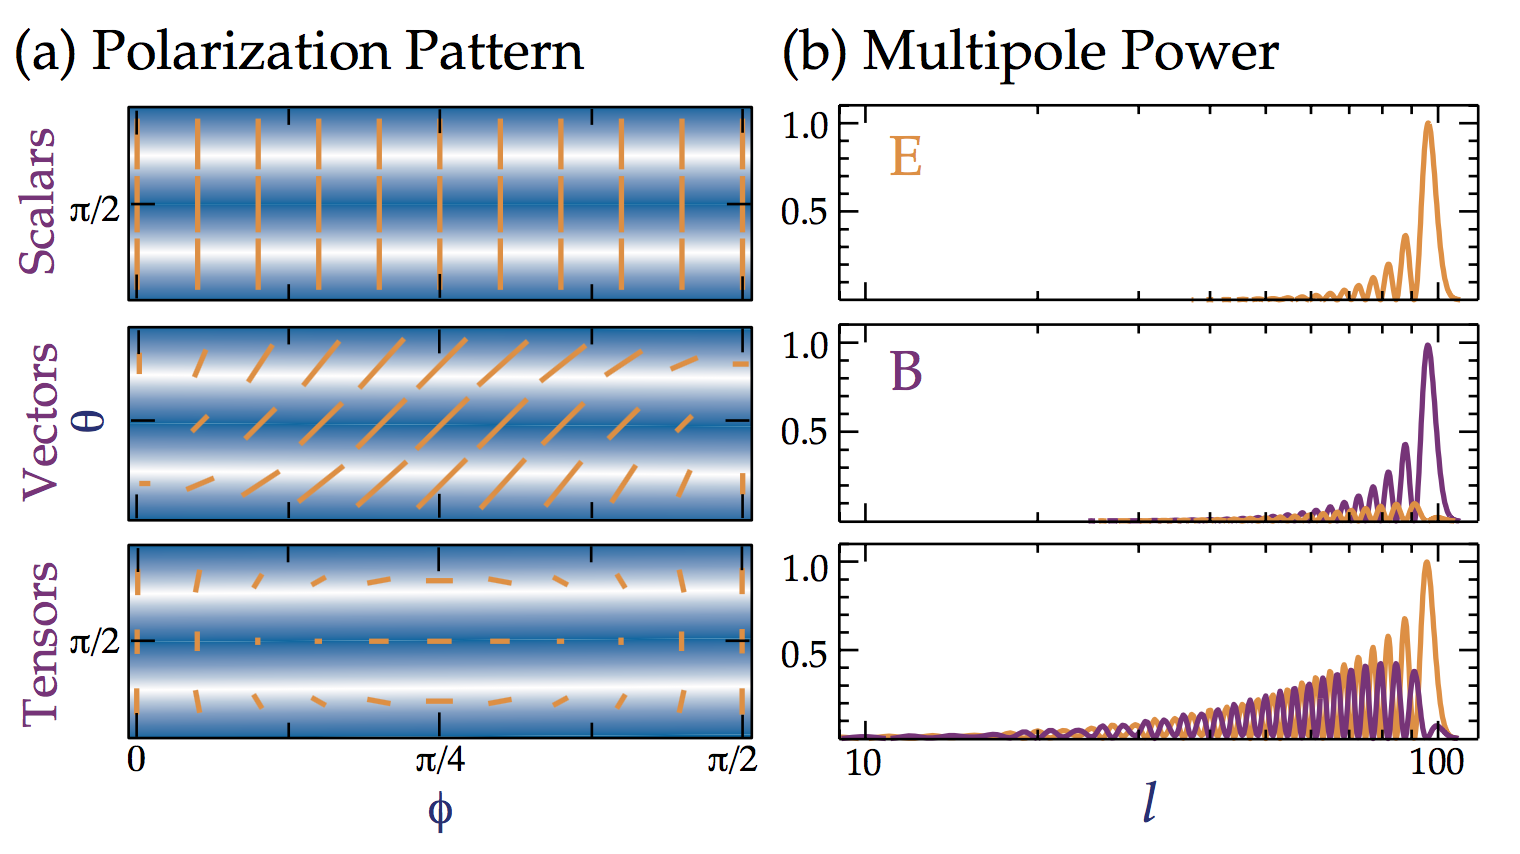
\includegraphics[width=16cm]{figures/cosmology/PolPatterns.png}
    \caption{\footnotesize{The $E$ and $B$ components of a plane wave perturbation. (a) Modulation of the local $E$-quadrupole pattern (yellow) from scattering by a plane wave. Modulation in the direction of (or orthogonal to) the polarization generates an $E$-mode with higher $\ell$; modulation in the crossed ($45^\circ$) direction generates a $B$-mode with higher $\ell$. Scalars generate only $E$-modes, vectors mainly $B$-modes, and tensors comparable amounts of both. (b) Distribution of power in a single plane wave with $kr=100$ in multipole $\ell$ from the addition of spin and orbital angular momentum. Features in the power spectrum can be read directly off the pattern in (a). Image taken from Hu \& White (1997).}}
    \label{fig:polpatterns}
\end{figure}

{\noindent}These qualitative considerations can be quantified by noting that plane wave modulation simply represent the addition of angular momentum from the plane wave ($Y_\ell^0$) with the local spin angular dependence. The result is that plane wave modulation takes the $\ell=2$ local angular dependence to higher $\ell$ (smaller angles) and splits the signal into $E$ and $B$ components with ratios which are related to Clebsch-Gordan coefficients. At short wavelengths, these ratios are $B/E=0$, $6$, $8/13$ in power for scalars, vectors, and tensors (see Figure \ref{fig:polpatterns}b and Hu \& White 1997).

{\noindent}The distribution of power in multipole $\ell$-space is also important. Due to projection, a single plane wave contributes to a range of angular scales  $\ell\lesssim kr$ where $r$ is the comoving distance to the last scattering surface. From Figure \ref{fig:cmbquad}, we see that the smallest angular, largest $\ell\approx kr$ variations occur on lines of sight $\bm{\hat{n}}\cdot\bm{\hat{k}}=0$ or $\theta=\pi/2$ though a small amount of power projects to $\ell\ll kr$ as $\theta\rightarrow0$. The distribution of power in multipole space of Figure \ref{fig:polpatterns}b can be read directly off the local polarization pattern. In particular, the region near $\theta=\pi/2$ shown in Figure \ref{fig:polpatterns}a determines the behavior of the main contribution to the polarization power spectrum.

{\noindent}The full power spectrum is of course obtained by summing these plane wave contributions with weights dependent on the source of the perturbations and the dynamics of their evolution up to last scattering. Sharp features in the $k$-power spectrum will be preserved in the multipole power spectrum to the extent that the projectors in Figure \ref{fig:polpatterns}b approximate delta functions. For scalar $E$-modes, the sharpness of the projection is enhanced due to strong $Q$-contributions near $\theta=\pi/2$ $(\ell\sim kr)$ that then diminish as $\theta\rightarrow0$ $(\ell\ll kr)$. The same enhancement occurs to a lesser extent for vector $B$-modes due to $U$ near $\pi/2$ and tensor $E$-modes due to $Q$ there. On the other hand, a suppression occurs for vector $E$ and tensor $B$-modes due to the absence of $Q$ and $U$ at $\pi/2$ respectively. These considerations have consequences for the sharpness of features in the polarization power spectrum, and the generation of asymptotic ``tails'' to the polarization spectrum at low-$\ell$ (see Hu \& White 1997) .

% --------------------------------------------------------------
%
%                           18. 
%
% --------------------------------------------------------------

\newpage
\subsection{Question 18}

What are the similarities and differences between the cosmic neutrino background and the cosmic microwave background?

\subsubsection{Short answer}

Just as the CMB is a relic of the time when the Universe was opaque to photons, the CNB is a relic of the time when the Universe was hot and dense enough to be opaque to neutrinos.

{\noindent}The number density of each of the three flavors of neutrinos ($\nu_e$, $\nu_\mu$, and $\nu_\tau$) has been calculated to be 3/11 times the number density of CMB photons. This means that at any moment, about twenty million cosmic neutrinos are zipping through your body.

\subsubsection{Additional context}

Additional context.

\subsubsection{Follow-up Questions}

\begin{itemize}
    \item What is a neutrino?
    \item How do we determine their mass?
    \item Besides the sun and the CNB, what other sources of neutrinos are there?
    \item What is the neutrino contribution to the density of the Universe?
    \item Why do neutrinos decouple at 1 second (i.e., before photons)?
\end{itemize}


% --------------------------------------------------------------
%
%                           19. 
%
% --------------------------------------------------------------

\newpage
\subsection{Question 19}

What is the difference between an isocurvature mode and an adiabatic mode, in terms of the initial density perturbations in the early universe? How do we know that the initial conditions are mostly adiabatic?

\subsubsection{Short answer}

Answer.

\subsubsection{Additional context}

In a complete description of energy density perturbations, the total energy density of the Universe includes components of baryonic matter ($\rho_b$), dark matter ($\rho_c$), radiation ($\rho_\mathrm{rad}$), and dark energy ($\rho_\Lambda$):

\begin{align*}
    \rho(\mathbf{x},t) = \rho_b(\mathbf{x},t) + \rho_c(\mathbf{x},t) + \rho_\mathrm{rad}(\mathbf{x},t) + \rho_\Lambda(\mathbf{x},t).
\end{align*}

{\noindent}In terms of their global gravitational influence, dark matter and baryonic matter contribute and evolve equivalently, therefore on cosmological scales they can be combined into a total matter energy density $\rho_m = \rho_b + \rho_c$. Each component may have its own (primordial) perturbation character. Dark energy does not have any density fluctuations, so $\delta_\Lambda(\mathbf{x},t) = 0$. Since most of the structure formation happened during the \textit{matter-dominated era}, this mainly involves the evolution of matter linear perturbations $\delta_m(\mathbf{x},t)$.

{\noindent}Cosmological perturbations will evolve quite differently for different \textit{perturbation modes}, each of which are identified on the basis of the nature of radiation perturbations with respect to matter perturbations. \textit{Isothermal perturbation modes} only involve matter perturbations ($\delta_m$) while radiation remains uniformly distributed throughout the 
Universe ($\delta_\mathrm{rad} = 0$). On the other hand, the primordial perturbations $\delta_m$ and $\delta_\mathrm{rad}$ may be completely equivalent (except for a constant proportionality factor) corresponding to zero fluctuations in entropy; these are \textit{adiabatic perturbation modes}. A third type of perturbation is that of \textit{isocurvature perturbation modes} in which radiation and matter perturbations cancel each other out such that the local curvature remains equal to the global cosmological curvature. Moreover, the evolution of the various components is complicated to a considerable extent by their mutual interactions. A simple illustration is that of baryonic matter initially without density perturbations: while dark matter creates even deeper potential wells, baryonic matter will fall in and experience increasingly stronger perturbations. Also, in pre-recombination epoch, baryonic matter is closely coupled to radiation such that its evolution is seriously affected by the corresponding radiation pressure gradients.

% --------------------------------------------------------------
%
%                           20. 
%
% --------------------------------------------------------------

\newpage
\subsection{Question 20}

Give three examples of possible dark matter candidates (current or historical). What is their status observationally?

\subsubsection{Short answer}

Answer.

\subsubsection{Additional context}

Additional context.

\subsubsection{Follow-up Questions}

\begin{itemize}
    \item How do neutrinos fit into this picture? (listed were MACHOs, axions and WIMPS)
    \item HDM versus CDM.
    \item What is MOND and how does it fit in with DM?
    \item What happens if we don't find WIMPs? How is this search going?
\end{itemize}

% --------------------------------------------------------------
%               Resources 
% --------------------------------------------------------------

\newpage
\subsection{Resources}

\begin{itemize}
    \item Extragalactic Astronomy and Cosmology; Shneider (2006)
    \item Introduction to Cosmology; Ryden (2006)
    \item From First Light to Reionization; Stiavelli (2009)
    \item Modern Cosmology, Dodelson (2003)
    \item 21-cm Cosmology in the 21st Century; Pritchard \& Loelo (2012)
    \item Distance Measures in Cosmology; Hogg (2000)
    \item A CMB Polarization Primer; Hu \& White (1997)
    \item Big Bang Nucleosynthesis; Fields \& Olive (2006)
    \item Cosmic Microwave Background Anisotropies; Hu \& Dodelson (2002)
    \item Lecture Notes on CMB Theory; From Nucleosynthesis to Recombination, Hu (2008)
    \item Observational Probes of Cosmic Acceleration; Weinberg et al. (2013)
    \item Particle Dark Matter: Evidence, Candidates, and Constraints; Bertone et al. (2005)
    \item Observational Constraints on Cosmic Reionization; Fan et al. (2006)
    \item Cosmology with the Sunyaev-Zel'dovich Effect; Carlstrom et al. (2002)
    \item Tired Light and the ``Missing Mass'' Problem; Yourgrau \& Woodward (1971)
    \item On the Robustness of the Acoustic Scale in the Low-Redshift Clustering of Matter; Eisenstein et al. (2007)
    \item Detection of the Baryon Acoustic Peak in the Large-Scale Correlation Function of SDSS Luminous Red Galaxies; Eisenstein et al. (2005)
\end{itemize}






































% --------------------------------------------------------------
%
%
%                              EXTRAGALACTIC 
%
%
% --------------------------------------------------------------

\newpage
\section{Extragalactic Astronomy}

% --------------------------------------------------------------
%               1. 
% --------------------------------------------------------------

\subsection{Question 1}

Sketch out the Hubble sequence. What physical trends are captured by the classification system?

\subsubsection{Short answer}

\begin{figure}[h]
    \centering
    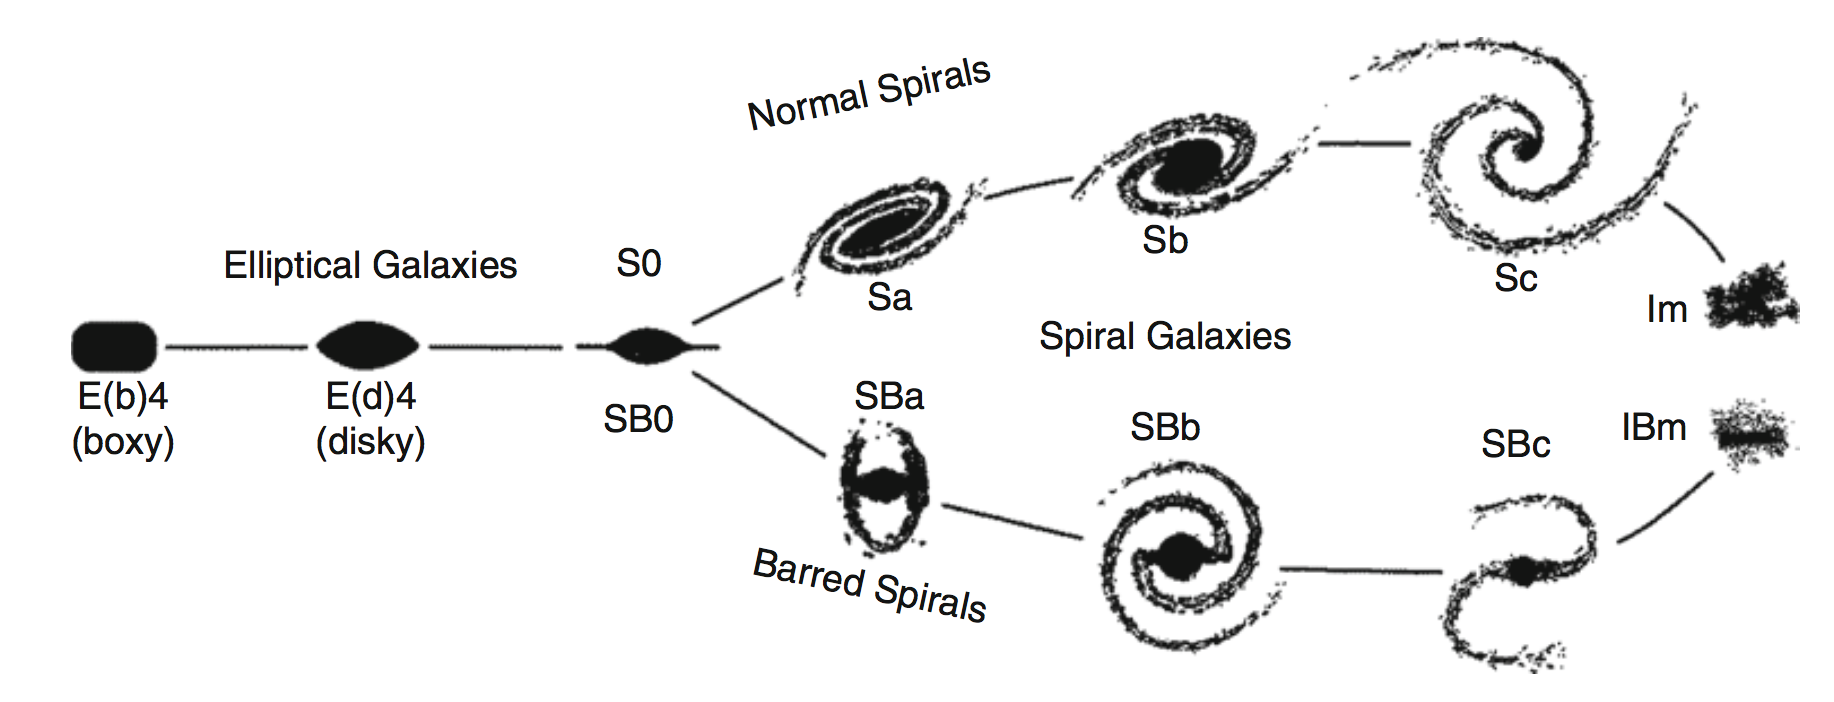
\includegraphics[width=16cm]{figures/extragalactic/HubbleSequence.png}
    \caption{\footnotesize{Hubble’s `tuning fork' for galaxy classification. Adapted from: J. Kormendy \& R. Bender 1996, A Proposed Revision of the Hubble Sequence for Elliptical Galaxies, ApJ 464, L119, Fig. 1. Image taken from Schneider (2006).}}
    \label{fig:hubblesequence}
\end{figure}

\subsubsection{Additional context}

Historically, optical photometry was the method used to observe galaxies. Thus, the morphological classification defined by Hubble is still the best-known today. Besides morphological criteria, color indices, spectroscopic parameters (based on emission or absorption lines), the broad-band spectral distribution (galaxies with/without radio- and/or X-ray emission, or emission in the infrared), as well as other features may also be used.

{\noindent}Figure \ref{fig:hubblesequence} shows the classification scheme defined by Hubble. According to this, three main types of galaxies exist:

\begin{itemize}
    \item Elliptical galaxies (E's) are galaxies that have nearly elliptical isophotes without any clearly defined structure. They are subdivided according to their ellipticity $\epsilon\equiv1-b/a$, where $a$ and $b$ denote the semi-major and the semi-minor axes, respectively. Ellipticals are found over a relatively broad range in ellipticity, $0\geq\epsilon\geq0.7$. The notation E$n$ is commonly used to classify the ellipticals with respect to $\epsilon$, with $n=10\epsilon$; i.e., an E4 galaxy has an axis ratio of $b/a0.6$, and E0's have circular isophotes.
    \item Spiral galaxies consist of a disk with spiral arm structure and a central bulge. They are divided into two subclasses: normal spirals (S's) and barred spirals (SB's). In each of these subclasses, a sequence is defined that is ordered according to the brightness ratio of bulge and disk, and that is denoted by a, ab, b, bc, c, cd, d. Objects along this sequence are often referred to as being either an early- type or a late-type; hence, an Sa galaxy is an early-type spiral, and an SBc galaxy is a late-type barred spiral. It's stressed explicitly that this nomenclature is not a statement of the evolutionary stage of the objects but is merely a nomenclature of purely historical origin.
    \item Irregular galaxies (Irr’s) are galaxies with only weak (Irr I) or no (Irr II) regular structure. The classification of Irr's is often refined. In particular, the sequence of spirals is extended to the classes Sdm, Sm, Im, and Ir (m stands for Magellanic; the Large Magellanic Cloud is of type SBm).
    \item S0 galaxies are a transition between ellipticals and spirals which are also called lenticulars as they are lentil-shaped galaxies. They contain a bulge and a large enveloping region of relatively unstructured brightness which often appears like a disk without spiral arms. Ellipticals and S0 galaxies are referred to as early-type galaxies, spirals as late-type galaxies. As before, these names are only historical and are not meant to describe an evolutionary track!
\end{itemize}

{\noindent}Obviously, the morphological classification is at least partially affected by projection effects. If, for instance, the spatial shape of an elliptical galaxy is a triaxial ellipsoid, then the observed ellipticity will depend on its orientation with respect to the line-of-sight. Also, it will be difficult to identify a bar in a spiral that is observed from its side (`edge-on').

{\noindent}Besides the aforementioned main types of galaxy morphologies, others exist which do not fit into the Hubble scheme. Many of these are presumably caused by interaction between galaxies. Furthermore, we observe galaxies with radiation characteristics that differ significantly from the spectral behavior of `normal' galaxies.

{\noindent}In summary:

\begin{itemize}
    \item Most luminous galaxies in the local Universe fit onto the Hubble sequence; they are either ellipticals, spirals, or belong to the class of S0 galaxies, which shares some properties with the two other classes.
    \item Ellipticals and spirals differ not only in their morphology, but in several other respects, for example: (1) Spirals contain a sizable fraction of gas, whereas the gas-to- stellar mass ratio in ellipticals is much smaller. As a consequence, (2) spirals have ongoing star formation, ellipticals not, or only very little. As a further consequence, (3) the light of elliptical galaxies is substantially redder than that of spirals. Obviously, the morphology of galaxies and the properties of their stellar populations are strongly correlated.
    \item The stars in spirals have a very ordered motion, moving around the galactic center on nearly circular orbits in a common orbital plane, having a velocity dispersion that is much smaller than the orbital velocity; the stars in the disk are called `dynamically cold'. In contrast, the motion of stars in ellipticals is largely random, with fairly little coherent velocity; they are dynamically hot.
    \item Some elliptical galaxies show clear signs of complex structure, which are interpreted as indications of past interaction with other galaxies. In contrast, the disks of spirals are very thin, which means that they have been largely unperturbed for a long while in the past.
    \item The rotation curves of spiral galaxies are almost flat for large radii, in contrast to what would be expected from the visible mass distribution that declines exponentially outwards. This implies that there is more matter than seen in stars and gas -- the galaxies are embedded in a halo of dark matter. Whereas for elliptical galaxies the radial density distribution is more difficult to probe, the presence of dark matter has been verified also for ellipticals.
    \item Both spirals and ellipticals follow scaling relations which connect their luminous properties (luminosity or surface brightness) with their dynamical properties (rotational velocity or velocity dispersion). Hence, the formation and evolution of galaxies and their stellar populations must proceed in a way as to place them onto these scaling relations.
\end{itemize}

\subsubsection{Follow-up Questions}

\begin{itemize}
    \item What physical trends does the Hubble sequence show that were not explicitly encoded in it? (i.e., spiral arm tightness and bulge size are properties that Hubble based the sequence off of.)
    \item Are there any other physical properties that the Hubble sequence ended up telling us about (i.e., by `accident')?
\end{itemize}


% --------------------------------------------------------------
%               2. 
% --------------------------------------------------------------

\newpage
\subsection{Question 2}

What is the total mass (in both dark matter and in stars) of the Milky Way galaxy? How does this compare to M31 and to the LMC? How is this mass determined?

\subsubsection{Short answer}

Answer.

\subsubsection{Additional context}

Additional context.

\subsubsection{Follow-up Questions}

\begin{itemize}
    \item If rotation curve/lensing measurements were instead due to modified gravity, how could we tell?
    \item What are $\Omega_m$ and $\Omega_b$ estimated to be? Why does the ratio of the two differ from the star/total mass ratio you have here? Where is all the extra baryonic mass?
    \item When you say we estimate stellar mass by ``counting stars'', what does that mean?
\end{itemize}

% --------------------------------------------------------------
%               3. 
% --------------------------------------------------------------

\newpage
\subsection{Question 3}

Describe as many steps of the distance ladder and the involved techniques as you can. What are the rough distances to the Magellanic Clouds, Andromeda, and the Virgo Cluster?

\subsubsection{Short answer}

Answer.

\subsubsection{Additional context}

{\noindent}\textbf{Trigonometric parallax ($<30\,{\rm pc}$)}: The most important method of distance determination is the trigonometric parallax, not only from a historical point-of-view. This method is based on a purely geometric effect and is therefore independent of any physical assumptions. Due to the motion of the Earth around the Sun the positions of nearby stars on the sphere change relative to those of very distant sources (e.g., extragalactic objects such as quasars). The latter therefore define a fixed reference frame on the sphere. In the course of a year the apparent position of a nearby star follows an ellipse on the sphere, the semi-major axis of which is called the parallax. The axis ratio of this ellipse depends on the direction of the star relative to the ecliptic (the plane that is defined by the orbits of the Earth and the other planets). The parallax depends on the radius $r$ of the Earth’s orbit, hence on the Earth-Sun distance which is, by definition, one astronomical unit (AU). Furthermore, the parallax depends on the distance $d$ of the star,

\begin{align*}
    \frac{r}{d} = \tan(p) \approx p ~ [{\rm rad}].
\end{align*}

{\noindent}where we used $p\ll1$ in the last step, and $p$ is measured in radians as usual. The trigonometric parallax is also used to define the common unit of distance in astronomy: one parsec (pc) is the distance of a hypothetical source for which the parallax is exactly $p=1''$. With the conversion of arcseconds to radians ($1''\approx4.848\times10^{-6}\,{\rm rad}$) one gets $p/1''=206265p$, which for a parsec yields

\begin{align*}
    1\,{\rm pc} = 206265\,{\rm AU} = 3.086\times10^{16}\,{\rm m}.
\end{align*}

{\noindent}The distance corresponding to a measured parallax is then
calculated as

\begin{align*}
    d = \left(\frac{p}{1''}\right)^{-1}\,{[\rm pc]}.
\end{align*}

{\noindent}o determine the parallax p, precise measurements of the position of an object at different times are needed, spread over a year, allowing us to measure the ellipse drawn on the sphere by the object’s apparent position. For ground-based observations the accuracy of this method is limited by the atmosphere. The seeing causes a blurring of the images of astronomical sources and thus limits the accuracy of position measurements. From the ground this method is therefore limited to parallaxes larger than $\approx0.1''$, implying that the trigonometric parallax yields distances to stars only within $\approx30\,{\rm pc}$.

{\noindent}\textbf{Proper motions}: Stars are moving relative to us or, more precisely, relative to the Sun. To study the kinematics of the Milky Way we need to be able to measure the velocities of stars. The radial component $v_r$ of the velocity is easily obtained from the Doppler shift of spectral lines,

\begin{align*}
    v_r = \left(\frac{\Delta\lambda}{\lambda_0}\right)c ~ [{\rm m\,s^{-1}}]
\end{align*}

{\noindent}where $\lambda_)$ is the rest-frame wavelength of an atomic transition and $\Delta\lambda=\lambda-\lambda_0$ is the Doppler shift of the wavelength due to the radial velocity of the source. The sign of the radial velocity is defined such that $v_r>0$ corresponds to a motion away from us, i.e., to a redshift of spectral lines.

{\noindent}In contrast, the determination of the other two velocity components is much more difficult. The tangential component, $v_t$, of the velocity can be obtained from the proper motion of an object. In addition to the motion caused by the parallax, stars also change their positions on the sphere as a function of time because of the transverse component of their velocity relative to the Sun. The proper motion $\mu$ is thus an angular velocity, e.g., measured in milliarcseconds per year (mas/yr or $''/{\rm year}$). This angular velocity is linked to the tangential velocity component via

\begin{align*}
    v_t = d\mu = 4.74\left(\frac{d}{1\,{\rm pc}}\right) \left(\frac{\mu}{1''\,{\rm year^{-1}}}\right) ~ [{\rm m\,s^{-1}}].
\end{align*}

{\noindent}Therefore, one can calculate the tangential velocity from the proper motion and the distance. If the latter is derived from the trigonometric parallax, these can be combined to yield

\begin{align*}
    v_t = d\mu = 4.74 \left(\frac{\mu}{1\,''\,{\rm year^{-1}}}\right) \left(\frac{p}{1''}\right)^{-1} ~ [{\rm m\,s^{-1}}].
\end{align*}

{\noindent}Of course, the proper motion has two components, corresponding to the absolute value of the angular velocity and its direction on the sphere. Together with $v_r$ this determines the three-dimensional velocity vector. Correcting for the known velocity of the Earth around the Sun, one can then compute the velocity vector v of the star relative to the Sun, called the heliocentric velocity.

{\noindent}\textbf{Moving cluster parallax ($<200\,{\rm pc}$)}: The stars in an (open) star cluster all have a very similar spatial velocity. This implies that their proper motion vectors should be similar. To what accuracy the proper motions are aligned depends on the angular extent of the star cluster on the sphere. Like two railway tracks that run parallel but do not appear parallel to us, the vectors of proper motions in a star cluster also do not appear parallel. They are directed towards a convergence point, as depicted in Figure \ref{fig:clusterparallax}.

\begin{figure}[h]
    \floatbox[{\capbeside\thisfloatsetup{capbesideposition={right,top},capbesidewidth=4cm}}]{figure}[\FBwidth]
    {\caption{\footnotesize{The moving cluster parallax is a projection effect, similar to that known from viewing railway tracks. The directions of velocity vectors pointing away from us seem to converge and intersect at the convergence point. The connecting line from the observer to the convergence point is parallel to the velocity vector of the star cluster. Image taken from Schneider (2006).}}
    \label{fig:clusterparallax}}
    {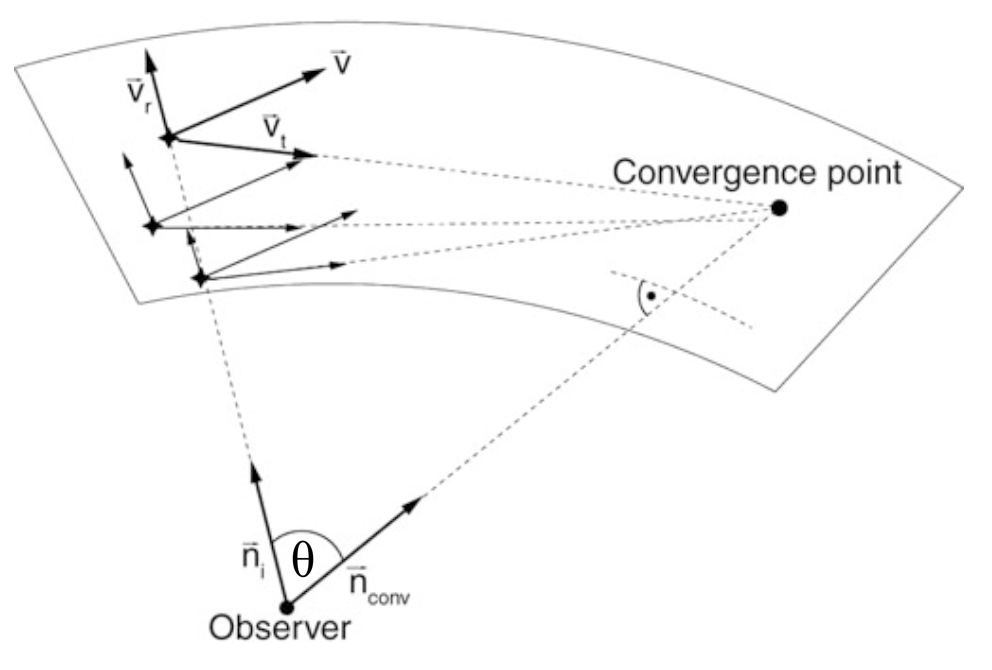
\includegraphics[width=10cm]{figures/extragalactic/ClusterParallax.png}}
\end{figure}

{\noindent}We consider a star cluster and assume that all stars have the same spatial velocity $v$. The position of the i-th star as a function of time is then described by

\begin{align*}
    \mathbf{r}_i(t) = \mathbf{r}_i(t) + \mathbf{v}t ~ [{\rm m}],
\end{align*}

{\noindent}where $\mathbf{r}_i$ is the current position if we identify the origin of time, $t=0$, with `today'. The direction of a star relative to us is described by the unit vector

\begin{align*}
    \mathbf{n}_i(t) \equiv \frac{\mathbf{r}_i}{\lvert\mathbf{r}_i\rvert} ~ [{\rm dimensionless}].
\end{align*}

{\noindent}From this, one infers that for large times, $t\rightarrow\infty$, the direction vectors of the convergence point are identical for all stars in the cluster,

\begin{align*}
    \mathbf{n}_i(t) \rightarrow \frac{\mathbf{v}}{\lvert\mathbf{v}\rvert} \equiv \mathbf{n}_\mathrm{conv} ~ [{\rm dimensionless}].
\end{align*}

{\noindent}Hence for large times all stars will appear at the same point $\mathbf{n}_\mathrm{conv}$: the convergence point. This only depends on the direction of the velocity vector of the star cluster. In other words, the direction vector of the stars is such that they are all moving towards the convergence point. Thus, $\mathbf{n}_\mathrm{conv}$ (and hence $\mathbf{v}/\lvert\mathbf{v}\rvert$) can be measured from the direction of the proper motions of the stars in the cluster. On the other hand, one component of $\mathbf{v}$ can be determined from the (easily measured) radial velocity $\mathbf{v}_r$. With these two observables the three-dimensional velocity vector $\mathbf{v}$ is completely determined, as is easily demonstrated: let $\theta$ be the angle between the line-of-sight $\mathbf{n}$ towards a star in the cluster and $\mathbf{v}$. The angle is directly read off from the direction vector $\mathbf{n}$ and the convergence point, $\cos\theta = \mathbf{n}\cdot\mathbf{v}/\lvert\mathbf{v}\rvert = \mathbf{}_\mathrm{conv}\cdot\mathbf{n}$. With $v\equiv\lvert\mathbf{v}\rvert$ one then obtains

\begin{align*}
    v_r = v\cos\theta ~ [{\rm m\,s^{-1}}], ~~~~~ v_t = v\sin\theta ~ [{\rm m\,s^{-1}}],
\end{align*}

{\noindent}and so

\begin{align*}
    v_t = v_r\cos\theta ~ [{\rm m\,s^{-1}}].
\end{align*}

{\noindent}This means that the tangential velocity $\mathbf{v}_t$ can be measured without determining the distance to the stars in the cluster. On the other hand, we have a relation between the proper motion, the distance, and $\mathbf{v}$. Hence, a distance determination for the star is now possible with

\begin{align*}
    \mu = \frac{v_t}{d} = \frac{v_r\tan\theta}{d} \rightarrow d = \frac{v_r\tan\theta}{\mu} ~ [{\rm pc}].
\end{align*}

{\noindent}This method yields accurate distance estimates of star clusters within $\sim200\,{\rm pc}$. The accuracy depends on the measurability of the proper motions. Furthermore, the cluster should cover a sufficiently large area on the sky for the convergence point to be well defined. For the distance estimate, one can then take the average over a large number of stars in the cluster if one assumes that the spatial extent of the cluster is much smaller than its distance to us.

{\noindent}\textbf{Main sequence fitting}: Most stars in the color-magnitude diagram (CMD) are located along the main sequence. This enables us to compile a calibrated main sequence of those stars whose trigonometric parallaxes are measured, thus with known distances. Utilizing photo- metric methods, it is then possible to derive the distance to a star cluster. 

{\noindent}The stars of a star cluster define their own main sequence (CMDs for some star clusters are displayed in Fig. 2.5); since they are all located at the same distance, their main sequence is already defined in a CMD in which only apparent magnitudes are plotted. This cluster main sequence can then be fitted to a calibrated main sequence by a suitable choice of the distance, i.e., by adjusting the distance modulus $m-M$,

\begin{align*}
    m_M = 5\log(d/{\rm pc}) - 5 ~ [{\rm mag}],
\end{align*}

{\noindent}where $m$ and $M$ denote the apparent and absolute magnitude, respectively.

{\noindent}In reality this method cannot be applied so easily since the position of a star on the main sequence does not only depend on its mass but also on its age and metallicity. Furthermore, only stars of luminosity class V (i.e., dwarf stars) define the main sequence, but without spectroscopic data it is not possible to determine the luminosity class.

{\noindent}\textbf{Extinction and reddening}: Another major problem is extinction. Absorption and scattering of light by dust affect the relation of absolute to apparent magnitude: for a given $M$, the apparent magnitude $m$ becomes larger (fainter) in the case of absorption, making the source appear dimmer. Also, since extinction depends on wavelength, the spectral energy distribution of the source is modified and the observed colour of the star changes. Because extinction by dust is always associated with such a change in colour, one can estimate the absorption -- provided one has sufficient information on the intrinsic colour of a source or of an ensemble of sources.

{\noindent}We consider the equation of radiative transfer for pure absorption or scattering:

\begin{align*}
    \frac{\mathrm{d}I_\nu}{\mathrm{d}s} = -\alpha_\nu I_\nu ~ [\rm erg\,s^{-1}\,cm^{-3}\,ster^{-1}\,Hz^{-1}],
\end{align*}

{\noindent}where $I_\nu$ is the specific intensity at frequency $\nu$, $\alpha_\nu$ is the absorption coefficient, and $s$ is the distance along the light beam.

{\noindent}This says that the amount by which the intensity of a light beam is diminished on a path of length $\mathrm{d}s$ is $\mathrm{d}s$. The absorption coefficient $\alpha_\nu$ is thus defined as the constant of proportionality. In other words, on the distance interval $\mathrm{d}s$, a fraction $\alpha_\nu\mathrm{d}s$ of all photons at frequency $\nu$ is absorbed or scattered out of the beam. The solution of the transport equation is obtained by writing it in the form $\mathrm{d}\ln I_\nu=\mathrm{d}I_\nu/I_\nu=-\alpha_\nu\mathrm{d}s$ and integrating from $0$ to $s$,

\begin{align*}
    \ln I_\nu(s)-\ln I_\nu(0) = -\int\limits_0^s \alpha_\nu(s')\mathrm{d}s \equiv \tau_\nu(s) ~ [\rm erg\,s^{-1}\,cm^{-2}\,ster^{-1}\,Hz^{-1}],
\end{align*}

{\noindent}where in the last step we defined the optical depth, $\tau_\nu$, which depends on frequency. This yields

\begin{align*}
    I_\nu(s) = I_\nu(0)e^{-\tau_\nu(s)} ~ [\rm erg\,s^{-1}\,cm^{-2}\,ster^{-1}\,Hz^{-1}].
\end{align*}

{\noindent}The specific intensity is thus reduced by a factor $e^{-\tau}$ compared to the case of no absorption taking place. Because of the relation between flux and magnitude $m=-2.5\log S+{\rm const}$ or $S\propto 10^{-0.4m}$, one has

\begin{align*}
    \frac{I_\nu}{I_{\nu,0}} = 10^{-0.4(m-m_0)} = e^{-\tau_\nu} = 10^{-\log(e)\tau_\nu} ~ [{\rm dimensionless}],
\end{align*}

{\noindent}or,

\begin{align*}
    A_\nu &\equiv m-m_0 = -2.5\log(I_\nu/I_{\nu,0}) ~ [{\rm mag}] \\
          &= 2.5\log(e)\tau_\nu ~ [{\rm mag}] \\
          &= 1.086\tau_\nu ~ [{\rm mag}].
\end{align*}

{\noindent}Here, $A_\nu$ is the extinction coefficient describing the change of apparent magnitude $m$ compared to that without absorption, $m_0$. Since the absorption coefficient $\alpha_\nu$ depends on frequency, absorption is always linked to a change in colour. This is described by the colour excess which is defined as follows:

\begin{align*}
    E(X-Y) \equiv A_X-A_Y = (X-X_0)-(Y-Y_0) = (X-Y)-(X_0-Y_0) ~ [{\rm mag}].
\end{align*}

{\noindent}The color excess describes the change of the color index $(X-Y)$, measured in two filters $X$ and $Y$ that define the corresponding spectral windows by their transmission curves. The ratio $A_X/A_Y=\tau_{\nu(X)/\tau_{\nu(Y)}}$ depends only on the optical properties of the dust or, more specifically, on the ratio of the absorption coefficients in the two frequency bands $X$ and $Y$ considered here. Thus, the color excess is proportional to the extinction coefficient,

\begin{align*}
    E(X-Y) = A_X-A_Y = A_X\left(1-\frac{A_Y}{A_X}\right) \equiv A_XR_X^{-1} ~ [{\rm mag}].
\end{align*}

{\noindent}where in the last step we introduced the factor of proportionality $R_X$ between the extinction coefficient and the colour excess, which depends only on the properties of the dust and the choice of the filters. Usually, one considers a blue and a visual filter and writes

\begin{align*}
    A_V = R_V E(B-V) ~ [{\rm mag}].
\end{align*}

{\noindent}For example, for dust in our Milky Way we have the characteristic relation

\begin{align*}
    A_{V,\mathrm{MWG}} = (3.1\pm0.1)E(B-V) ~ [{\rm mag}].
\end{align*}

{\noindent}This relation is not a universal law, but the factor of proportionality depends on the properties of the dust. They are determined, e.g., by the chemical composition and the size distribution of the dust grains. Figure \ref{fig:extinctioncurve} shows the wavelength dependence of the extinction coefficient for different kinds of dust, corresponding to different values of $R_V$ . In the optical part of the spectrum we have approximately $\tau_\nu\propto\nu$, i.e., blue light is absorbed (or scattered) more strongly than red light. The extinction therefore always causes a reddening.

\begin{figure}[h]
    \floatbox[{\capbeside\thisfloatsetup{capbesideposition={right,top},capbesidewidth=4cm}}]{figure}[\FBwidth]
    {\caption{\footnotesize{Wavelength dependence of the extinction coefficient $A_\nu$, normalized to the extinction coefficient $A_I$ at $\lambda=9000$\,\AA$ = 0.9\,\mu$m. Different kinds of clouds, characterized by the value of $R_V$, i.e., by the reddening law, are shown. The solid curve specifies the mean Galactic extinction curve. The extinction coefficient, as determined from the observation of an individual star, is also shown. The figure insert shows a detailed plot at relatively large wavelengths in the NIR range of the spectrum; at these wavelengths the extinction depends only weakly on the value of $R_V$. Source: B. Draine 2003, Interstellar Dust Grains, ARA\&A 41, 241. Image taken from Schneider (2006).}}
    \label{fig:extinctioncurve}}
    {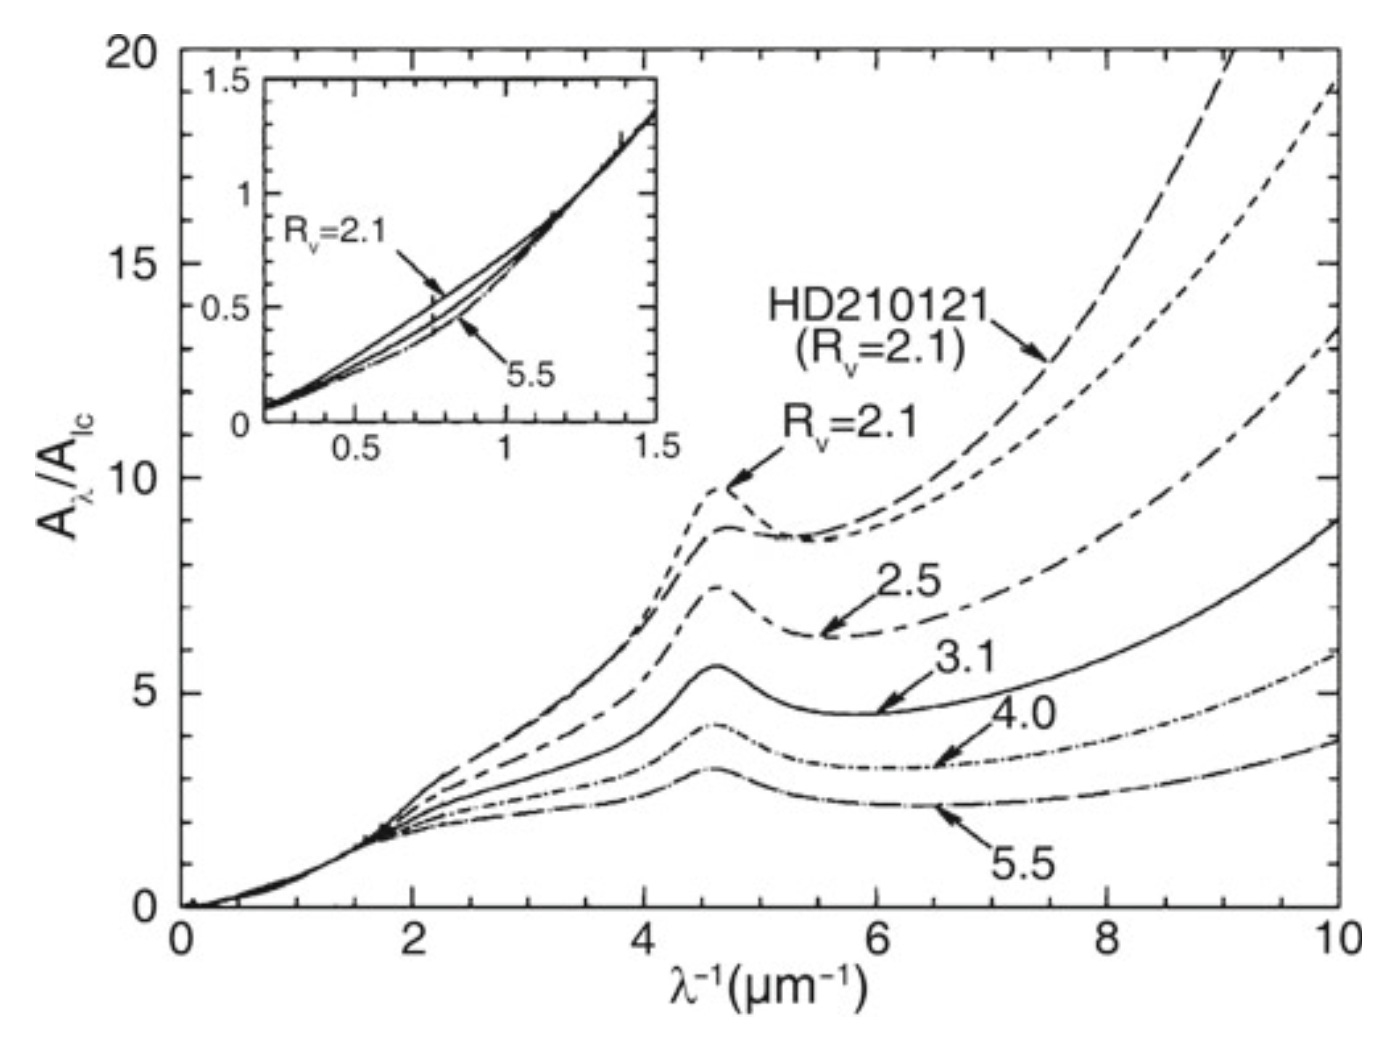
\includegraphics[width=12cm]{figures/extragalactic/ExtinctionCurve.png}}
\end{figure}

{\noindent}The extinction coefficient $A_V$ is proportional to the optical depth towards a source and so is the colour excess. Since the extinction is due to dust along the line-of-sight, the colour excess is proportional to the column density of dust towards the source. If we assume that the dust-to-gas ratio in the interstellar medium does not vary greatly, we expect that the column density of neutral hydrogen $N_\mathrm{H}$ is proportional to the colour excess. The former can be measured from the Lyman-$\alpha$ absorption in the spectra of stars, whereas the latter is obtained by comparing the observed colour of these stars with the colour expected for the type of star, given its spectrum (and thus, its spectral classification). One finds indeed that the color excess is proportional to the HI column density with

\begin{align*}
    E(B-V) = 1.7 \left(\frac{N_\mathrm{H}}{10^{22}\,{\rm atoms\,cm^{-2}}}\right) ~ [{\rm mag}],
\end{align*}

{\noindent}and a scatter of about 30\% around this relation. The fact that this scatter is so small indicates that the assumption of a constant dust-to-gas ratio is reasonable.

{\noindent}In the Solar neighborhood the extinction coefficient for sources in the disk is about

\begin{align*}
    A_V \approx \frac{d}{1\,{\rm kpc}} ~ [{\rm mag}],
\end{align*}

{\noindent}but this relation is at best a rough approximation, since the absorption coefficient can show strong local deviations from this law, for instance in the direction of molecular clouds.

{\noindent}\textbf{Colour-colour diagram}: As a first step in this measurement, it is necessary to determine the degree of extinction, which can only be done by analyzing the reddening. The stars of the cluster are plotted in a color-color diagram, for example by plotting the colors $(U-B)$ versus $(B-V)$. A colour-colour diagram also shows a main sequence along which the majority of the stars are aligned. The wavelength-dependent extinction causes a reddening in both colors. This shifts the positions of the stars in the diagram. The direction of the reddening vector depends only on the properties of the dust and is here assumed to be known, whereas the amplitude of the shift depends on the extinction coefficient. In a similar way to the CMD, this amplitude can now be determined if one has access to a calibrated, unreddened main sequence for the colour-colour diagram which can be obtained from the examination of nearby stars. From the relative shift of the main sequence in the two diagrams one can then derive the reddening and thus the extinction. The essential point here is the fact that the colour-colour diagram is \textit{independent of the distance}.

{\noindent}This then defines the procedure for the distance determination of a star cluster using photometry: in the first step we determine the reddening $E(B-V)$, and thus also $A_V$ via $A_V=(3.1\pm0.1)E(B-V)$ for the Galactic medium, by shifting the main sequence in a colour-colour diagram along the reddening vector until it matches a calibrated main sequence. In the second step the distance modulus is determined by vertically (i.e., in the direction of $M$) shifting the main sequence in the CMD until it matches a calibrated main sequence. From this, the distance is finally obtained according to

\begin{align*}
    m-M = 5\log\left(\frac{d}{1\,{\rm pc}}\right)-5+A ~ [{\rm mag}].
\end{align*}

{\noindent}\textbf{Spectroscopic distance}: From the spectrum of a star, the spectral type as well as its luminosity class can be obtained. The former is determined from the strength of various absorption lines in the spectrum, while the latter is obtained from the width of the lines. From the line width the surface gravity of the star can be derived, and from that its radius (more precisely, $M/R2^2$). The spectral type and the luminosity class specify the position of the star in the HRD unambiguously. By means of stellar evolution models, the absolute magnitude $M_V$ can then be determined. Furthermore, the comparison of the observed colour with that expected from theory yields the color excess $E(B-V)$, and from that we obtain $A_V$. With this information we are then able to determine the distance using

\begin{align*}
    m_V-A_V-M_V = 5\log\left(\frac{d}{1\,{\rm pc}}\right)-5 ~ [{\rm mag}].
\end{align*}

{\noindent}\textbf{Visual binaries}: Kepler’s third law for a two-body problem,

\begin{align*}
    P = \sqrt{\frac{4\pi^2}{G(m_1+m_2)}a^3} ~ [{\rm yr}]
\end{align*}

{\noindent}relates the orbital period $P$ of a binary star to the masses $m_i$ of the two components and the semi-major axis $a$ of the ellipse. The latter is defined by the separation vector between the two stars in the course of one period. This law can be used to determine the distance to a visual binary star. For such a system, the period $P$ and the angular diameter $2\theta$ of the orbit are direct observables. If one additionally knows the mass of the two stars, for instance from their spectral classification, $a$ can be determined according to Kepler's third law, and from this the distance follows with the small angle approximation $d=a/\theta$.

{\noindent}\textbf{Variable stars}: Several types of pulsating stars show periodic changes in their brightnesses, where the period of a star is related to its mass, and thus to its luminosity. This period-luminosity (PL) relation is ideally suited for distance measurements: since the determination of the period is independent of distance, one can obtain the luminosity directly from the period if the calibrated PL-relation is known. The distance is thus directly derived from the measured magnitude using the photometric distance, if the extinction can be determined from color measurements.

{\noindent}The existence of a relation between the luminosity and the pulsation period can be expected from simple physical considerations. Pulsations are essentially radial density waves inside a star that propagate with the speed of sound, $c_s$. Thus, one can expect that the period is comparable to the sound crossing time through the star, $P\sim R/c_s$. The speed of sound $c_s$ in a gas is of the same order of magnitude as the thermal velocity of the gas particles, so that $k_BT\sim m_pc_s^2$, where $m_p$ is the proton mass (and thus a characteristic mass of particles in the stellar plasma) and $k_B$ is Boltzmann's constant. According to the virial theorem, one expects that the gravitational binding energy of the star is about twice the kinetic (i.e., thermal) energy, so that for a proton,

\begin{align*}
    \frac{GMm_p}{R} \sim k_BT.
\end{align*}

{\noindent}Combining these relations, we obtain for the pulsation period

\begin{align*}
    P\sim\frac{R}{c_s}\sim\frac{R\sqrt{m_p}}{\sqrt{k_BT}} \sim\frac{R^{3/2}}{\sqrt{GM}} \propto \langle\rho\rangle^{-1/2},
\end{align*}

{\noindent}where $\langle\rho\rangle$ is the mean density of the star. This is a remarkable result -- the pulsation period depends only on the mean density. Furthermore, the stellar luminosity is related to its mass by approximately $L/M^33$. If we now consider stars of equal effective temperature $T_\mathrm{eff}$ (where $L\propto R^2T_\mathrm{eff}^4$), we find that

\begin{align*}
    P \propto \frac{R^{3/2}}{\sqrt{M}} \propto L^{7/12},
\end{align*}

{\noindent}which is the relation between period and luminosity that we were aiming for.

{\noindent}One finds that a well-defined period-luminosity relation exists for three types of pulsating stars:

\begin{itemize}
    \item $\delta$ Cepheid stars (classical Cepheids). These are young stars found in the disk population (close to the Galactic plane) and in young star clusters.
    \item W Virginis stars, also called population II Cepheids. These are low-mass, metal-poor stars located in the halo of the Galaxy, in globular clusters, and near the Galactic center.
    \item RR Lyrae stars. These are likewise population II stars and thus metal-poor. They are found in the halo, in globular clusters, and in the Galactic bulge.
\end{itemize}

{\noindent}\textbf{Globular clusters}: 

{\noindent}\textbf{Tully-Fisher relation}: Using $21\,{\rm cm}$ observations of spiral galaxies, in 1977 R. Brent Tully and J. Richard Fisher found that the maximum rotation velocity of spirals is closely related to their luminosity, following the relation

\begin{align*}
    L_\mathrm{TF} = \propto v_\mathrm{max}^\alpha ~ [{\rm erg\,s^{-1}}],
\end{align*}

{\noindent}where the power-law index (i.e., the slope) of the Tully-Fisher relation is about $\alpha\sim4$. The larger the wavelength of the filter in which the luminosity is measured, the smaller the dispersion of the Tully-Fisher relation (see Figure \ref{fig:tullyfisher}). This is to be expected because radiation at larger wavelengths is less affected by dust absorption and by the current star formation rate, which may vary to some extent between individual spirals. Furthermore, it is found that the value of $\alpha$ increases with the wavelength of the filter: The Tully-Fisher relation is steeper in the red, which follows from the fact that more massive, or more luminous galaxies (i.e., those with larger $v_\mathrm{,ax}$) are redder. The dispersion of galaxies around this relation in the NIR (e.g., in the H-band) is about 10\%.

\begin{figure}[h]
\floatbox[{\capbeside\thisfloatsetup{capbesideposition={right,top},capbesidewidth=4cm}}]{figure}[\FBwidth]
{\caption{\footnotesize{The Tully-Fisher relation for galaxies in the Local Group (dots), in the Sculptor group (triangles), and in the M81 group (squares). The absolute magnitude is plotted as a function of the width of the $21\,{\rm cm}$ profile which indicates the maximum rotation velocity. Filled symbols represent galaxies for which independent distance estimates were obtained, either from RR Lyrae stars, Cepheids, or planetary nebulae. For galaxies represented by open symbols, the average distance of the respective group is used. The solid line is a fit to similar data for the Ursa-Major cluster, together with data of those galaxies for which individual distance estimates are available (filled symbols). The larger dispersion around the mean relation for the Sculptor group galaxies is due to the group’s extent along the line-of-sight. Source: M.J. Pierce \& R.B. Tully 1992, Luminosity-line width relations and the extragalactic distance scale. I-Absolute calibration, ApJ 387, 47, p. 51, Fig. 1. Image taken from Schneider (2006).}}
\label{fig:tullyfisher}}
{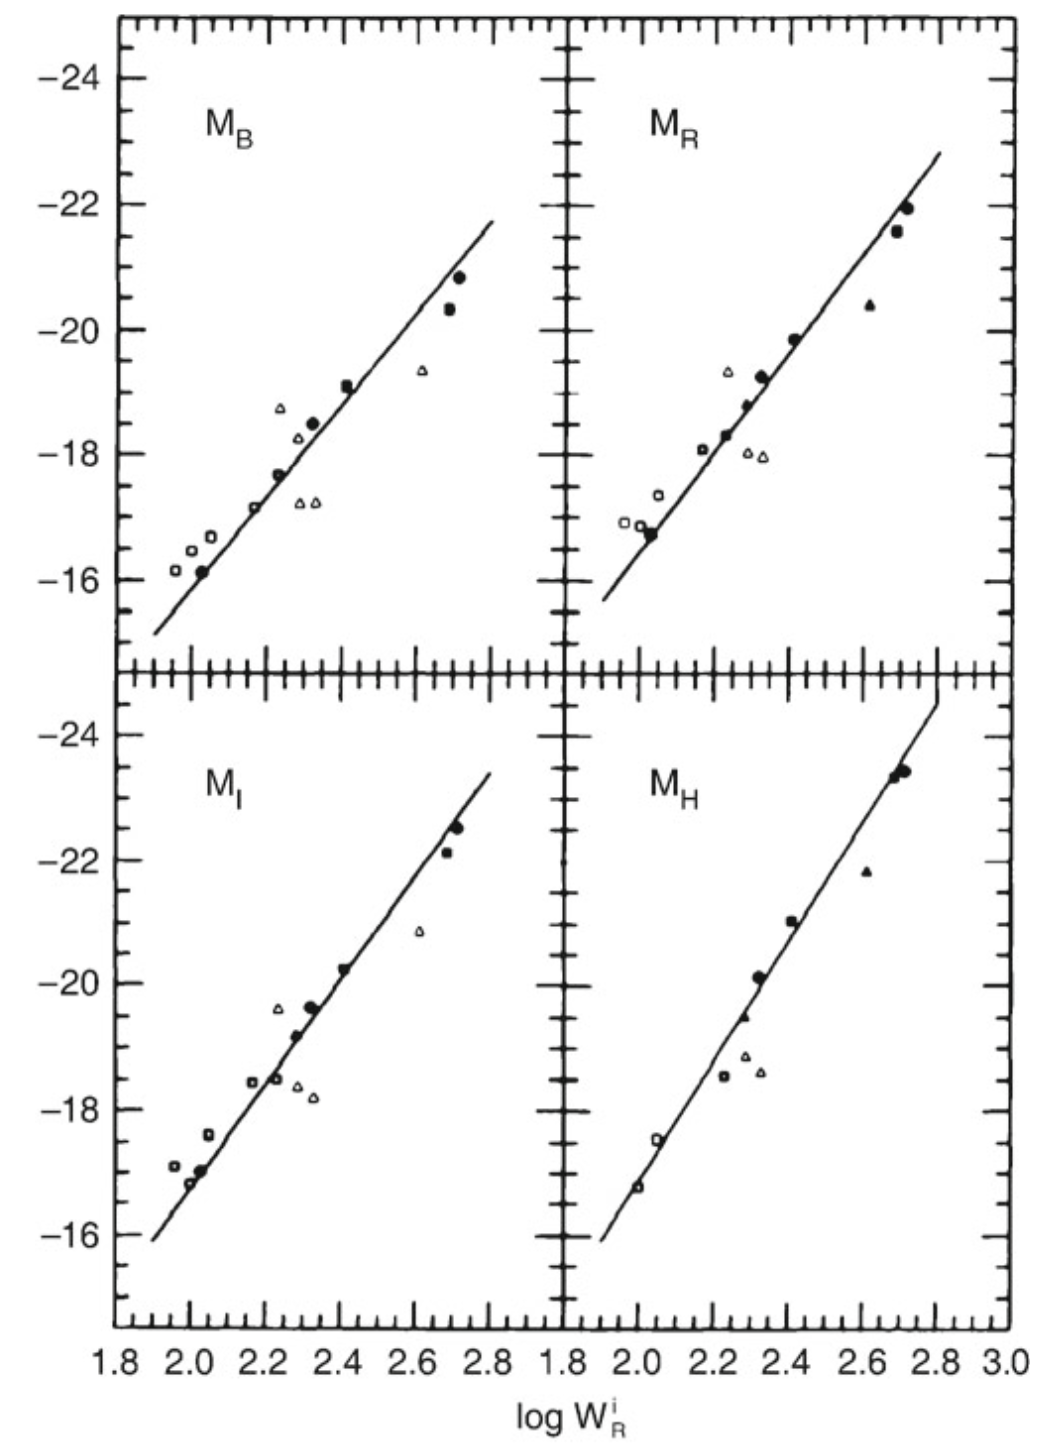
\includegraphics[width=12cm]{figures/extragalactic/TullyFisher.png}}
\end{figure}

{\noindent}Because of this close correlation, the luminosity of spirals can be estimated quite precisely by measuring the rotational velocity. The determination of the (maximum) rotational velocity is independent of the galaxy’s distance. By comparing the luminosity, as determined from the Tully-Fisher relation, with the measured flux, one can then estimate the distance of the galaxy -- without utilizing the Hubble relation!

{\noindent}The measurement of $v_\mathrm{max}$ is obtained either from a spatially resolved rotation curve, by measuring $v_\mathrm{rot}$, which can be done with optical spectroscopy or, for relatively nearby galaxies, also with spatially resolved $21\,{\rm cm}$ spectroscopy. Alternatively, one can observe an integrated spectrum of the $21\,{\rm cm}$ line of HI that has a Doppler width corresponding to about $2v_\mathrm{max}$ (see Fig.3.28). The Tully-Fisher relation shown in Figure \ref{fig:tullyfisher} was determined by measuring the width of the $21\,{\rm cm}$ line.

\begin{figure}[h]
    \floatbox[{\capbeside\thisfloatsetup{capbesideposition={right,top},capbesidewidth=4cm}}]{figure}[\FBwidth]
    {\caption{\footnotesize{$21\,{\rm cm}$ profile of the galaxy NGC7331. The bold dots indicate $20$ and $50$\% of the maximum flux; these are of relevance for the determination of the line width from which the rotational velocity is derived. Source: L.M. Macri et al. 2000, A Database of Tully-Fisher Calibrator Galaxies, ApJS 128, 461, p. 467, Fig. 5. Image taken from Schneider (2006).}}
    \label{fig:21cmvrot}}
    {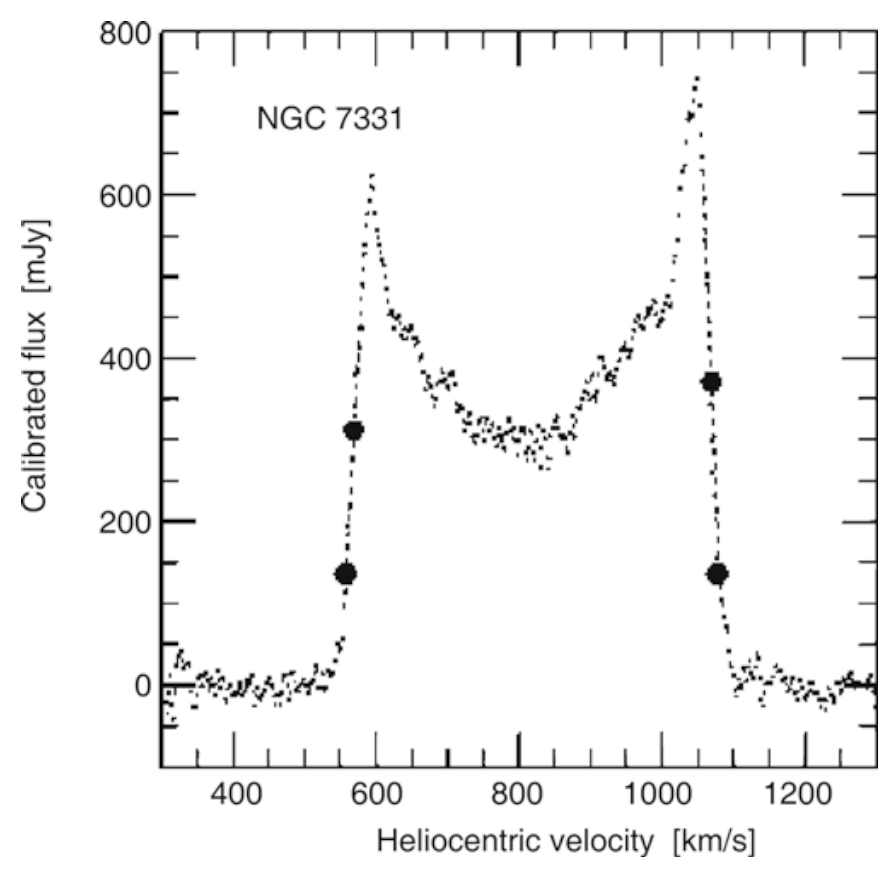
\includegraphics[width=8cm]{figures/extragalactic/21cm_vrot.png}}
\end{figure}

{\noindent}The shapes of the rotation curves of spirals are very similar to each other, in particular with regard to their flat behavior in the outer part. The flat rotation curve implies

\begin{align*}
    M = \frac{v_\mathrm{max}^2R}{G} ~ [{\rm M_\odot}],
\end{align*}

{\noindent}where the value of the distance $R$ from the center of the galaxy is chosen to be in the range of the flat part of the rotation curve (i.e., where $v_\mathrm{rot}(R)\approx v_\mathrm{max}$). We note that the exact value of $R$ is not important; of course, $M=M(R)$. By re-writing this,

\begin{align*}
    L = \left(\frac{M}{L}\right)^{-1} \frac{v_\mathrm{max}^2R}{G} ~ [{\rm erg\,s^{-1}}],
\end{align*}

{\noindent}and by replacing $R$ by the mean surface brightness $\langle I\rangle=L/R^2$, we obtain

\begin{align*}
    L = \left(\frac{M}{L}\right)^{-2} \left(\frac{1}{G^2\langle I\rangle}\right)v_\mathrm{max}^4 ~ [{\rm erg\,s^{-1}}].
\end{align*}

{\noindent}This is the Tully-Fisher relation if $M/L$ and $\langle I\rangle$ are the same for all spirals. The latter is in fact suggested by Freeman’s law. Since the shapes of rotation curves for spirals seem to be very similar, the radial dependence of the ratio of luminous to dark matter may also be quite similar among spirals. Furthermore, since the mass- to-light ratios of a stellar population as measured from the red or infrared emission do not depend strongly on its age, independently of their Hubble type. Within $R_{25}$ one finds $M/L_B=6.2$ for Sa's, $4.5$ for Sb's, and $2.6$ for Sc's. This trend does not come as a surprise because late types of spirals contain more young, blue and luminous stars.

{\noindent}\textbf{Faber-Jackson relation}: A relation for elliptical galaxies, analogous to the Tully-Fisher relation, was found by Sandra Faber and Roger Jackson. They discovered that the velocity dispersion in the center of ellipticals, $\sigma_v$, scales with luminosity,

\begin{align*}
    L_\mathrm{FJ} \propto \sigma_v^4 ~ [{\rm erg\,s^{-1}}]
\end{align*}

{\noindent}`Deriving' the Faber-Jackson scaling relation is possible under the same assumptions as for the Tully-Fisher relation. However, the dispersion of ellipticals about this relation is larger than that of spirals about the Tully-Fisher relation.

{\noindent}\textbf{$D_n-\sigma$ relation}: Another scaling relation for ellipticals which is of substantial importance in practical applications is the $D_n-\sigma$ relation. $D_n$ is defined as the mean diameter of an ellipse within which the average surface brightness. In corresponds to a value of $20.75\,{rm mag\,arcsec^{-2}}$ in the B-band. If we now assume that all ellipticals have a self-similar brightness profile, $I(R)=I_ef(R/R_r)$, with $f(1)=1$, then the luminosity within $D_n$ can be written as

\begin{align*}
    I_n\left(\frac{D_n}{2}\right)^2\pi &= 2\pi I_e \int\limits_0^{D_n/2} Rf(R/R_e)\mathrm{d}R \\
    &= 2\pi I_eR_e^2 \int\limits_0^{D_n/(2R_e)} ~ [{\rm erg\,s^{-1}\,m^{-2}}] xf(x)\mathrm{d}x,
\end{align*}

{\noindent}where in the last step we changed the integration variable to $x=R/R_e$. For a de Vaucouleurs profile we have approximately $f(x)\propto x^{-1.2}$ in the relevant range of radius. Computing the integral with this expression, we obtain

\begin{align*}
    D_n \propto R_eI_e^{0.8}.
\end{align*}

{\noindent}Empirically, we find that ellipticals follow the normalized $D_n-\sigma$ relation

\begin{align*}
    D_n = 2.05\times\left(\frac{\sigma_v}{100\,km\,s^{-1}}\right) ~ [{\rm kpc}]
\end{align*}

{\noindent}and they scatter around this relation with a relative width of about 15\%.

{\noindent}\textbf{Type Ia supernovae}: 


% --------------------------------------------------------------
%               4. 
% --------------------------------------------------------------

\newpage
\subsection{Question 4}

What evidence is there that most galaxies contain nuclear black holes? How do those black holes interact with their host galaxies?

\subsubsection{Short answer}

Answer.

\subsubsection{Additional context}

Additional context.

\subsubsection{Follow-up Questions}

\begin{itemize}
    \item Does heating from AGN affect star formation in the outer parts of the disk?
\end{itemize}

% --------------------------------------------------------------
%               5. 
% --------------------------------------------------------------

\newpage
\subsection{Question 5}

Define and describe globular clusters. Where are they located? What are their typical ages, and how is this determined?

\subsubsection{Short answer}

Answer.

\subsubsection{Additional context}

The visible halo of our Galaxy consists of about 150 globular clusters and field stars with a high velocity component perpendicular to the Galactic plane. Even at about 150, the number of known globular clusters is relatively small. A globular cluster is a collection of typically several hundred thousand stars, contained within a spherical region of radius   $\sim20\,{\rm pc}$. The stars in the cluster are gravitationally bound and orbit in the common gravitational field. The old globular clusters with $[Fe/H]<-0.8$ have an approximately spherical distribution around the Galactic center. A second population of globular clusters exists that contains younger stars with a higher metallicity, $[Fe/H]>-0.8$. They have a more oblate geometrical distribution and are possibly part of the thick disk because they show roughly the same scale-height.

{\noindent}Most globular clusters are at a distance of $r\lesssim35\,{\rm kpc}$ (with $r=\sqrt{R^2+z^2}$) from the Galactic center, but some are also found at $r>60\,{\rm kpc}$. At these distances it is hard to judge whether these objects are part of the Galaxy or whether they have been captured from a neighboring galaxy, such as the Magellanic Clouds.

{\noindent}The density distribution of metal-poor globular clusters and field stars in the halo is described by

\begin{align*}
    n(r)\propto r^{-\gamma},
\end{align*}

{\noindent}with a slope $\gamma$ in the range $3-3.5$.

{\noindent}The number of globular clusters is higher in early types and in more luminous galaxies. The specific abundance of globular clusters in a galaxy is defined as their number, normalized to a galaxy of absolute magnitude $M_V=-15$. This can be done by scaling the observed number $N_t$ of globular clusters in a galaxy of visual luminosity $L_V$ or absolute magnitude $M_V$, respectively, to that of a fiducial galaxy with $M_V$ corresponding to a luminosity of $L_V=L_{15}$:

\begin{align*}
    S_N = N_t\frac{L_{15}}{L_V} = N_t10^{0.4(M_V+15)}.
\end{align*}

{\noindent}If the number of globular clusters were proportional to the luminosity (and thus roughly to the stellar mass) of a galaxy, then this would imply a constant $S_N$ . However, this is not the case: For Sa's and Sb's we find $S_N\sim1.2$, whereas $S_N\sim0.5$ for Sc's. $S_N$ is larger for ellipticals and largest for cD galaxies.

{\noindent}There have been claims in the literature that even globular clusters contain a black hole; however, these claims are not undisputed. In addition, there may be objects that appear like globular clusters, but are in fact the stripped nucleus of a former dwarf galaxy. In this case, the presence of a central black hole is not unexpected.

\begin{figure}[t!]
    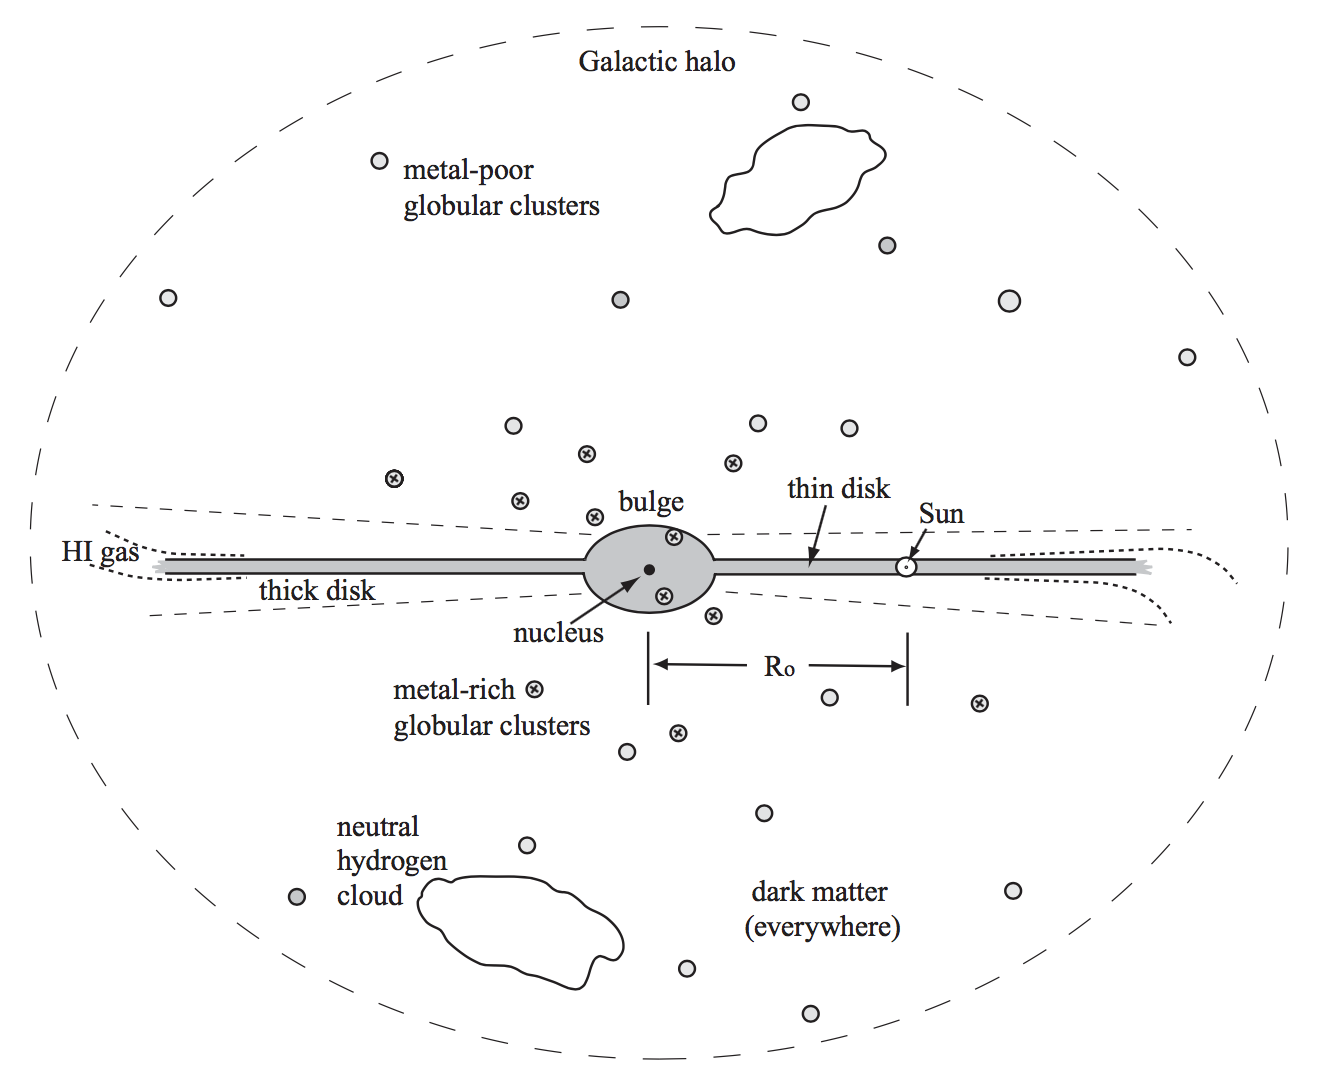
\includegraphics[width=14cm]{figures/extragalactic/MWGschematic.png}
    \centering
    \caption{A schematic side view of the Milky Way. Figure taken from Sparke (2007).}
    \label{fig:mwgschematic}
\end{figure}

\begin{figure}[t!]
    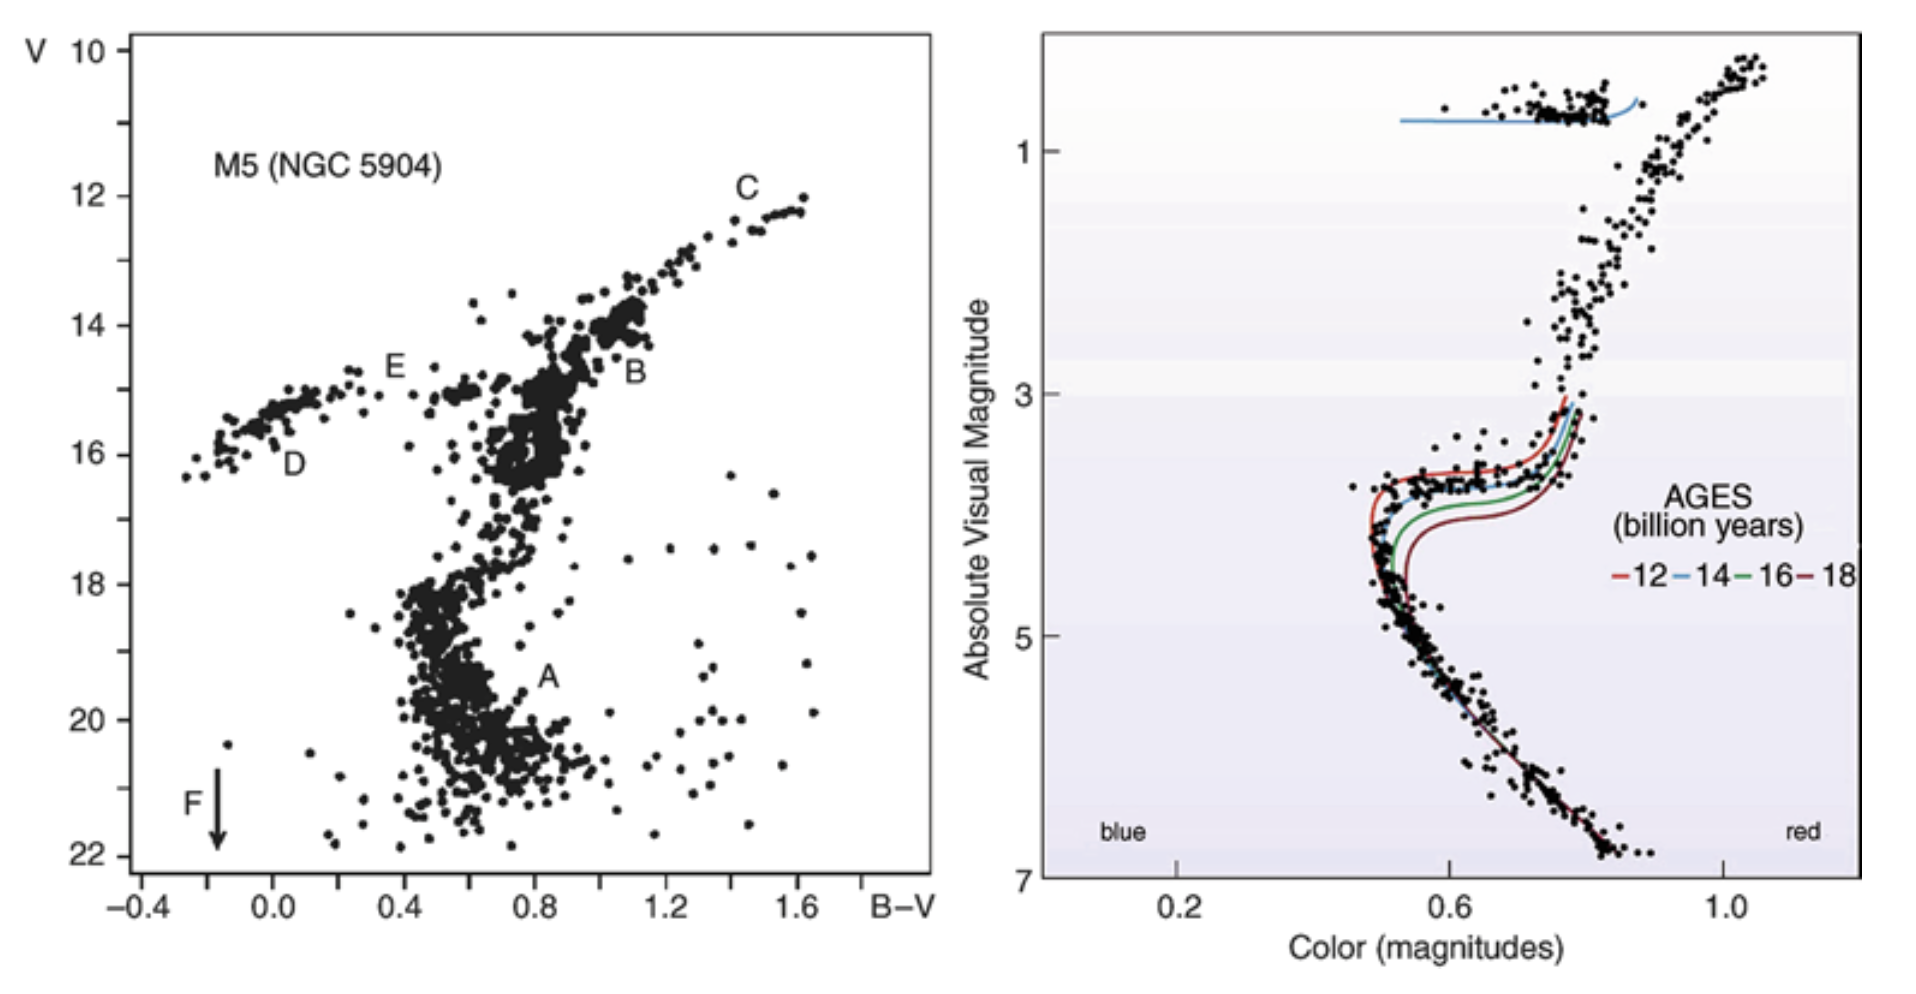
\includegraphics[width=16cm]{figures/extragalactic/GlobularClusters.png}
    \centering
    \caption{\footnotesize{Left: CMD of the globular cluster M5. The different sections are -- A: main sequence; B: red giant branch; C: point of He flash; D: horizontal branch; E: Schwarzschild-gap in the horizontal branch; F: white dwarfs, below the arrow. At the point where the MS turns over to the red giant branch (called the `turn-off point'), stars have a mass corresponding to a MS lifetime which is equal to the age of the globular cluster. Therefore, the age of the cluster can be determined from the position of the turn-off point by comparing it with models of stellar evolution. Right: Isochrones for different ages and compared to the stars of the globular cluster 47 Tucanae. Such analyses reveal that the oldest globular clusters in our Milky Way are about 12 billion years old. The age thus obtained also depends on the distance of the cluster. Credit: M5: c Leos Ondra; 47 Tuc: J.E. Hesser, W.E. Harris, D.A. Vandenberg, J.W.B. Allwright, P. Scott \& P.B. Stetson 1987. Figure taken from Schneider (2006).}}
    \label{fig:globularclusters}
\end{figure}

\subsubsection{Follow-up Questions}

\begin{itemize}
    \item Can you say something about collisional behavior in clusters?
    \item Why do or don't we think globular clusters have dark matter? How would we determine this? 
\end{itemize}

% --------------------------------------------------------------
%               6. 
% --------------------------------------------------------------

\newpage
\subsection{Question 6}

Describe three different methods used in the determination of the mass of a galaxy cluster.

\subsubsection{Short answer}

Answer.

\subsubsection{Additional context}

Additional context.

% --------------------------------------------------------------
%               7. 
% --------------------------------------------------------------

\newpage
\subsection{Question 7}

What is the density-morphology relation for galaxies? How is that related to what we know about the relationship between galaxy density and star formation rates in galaxies?

\subsubsection{Short answer}

Answer.

\subsubsection{Additional context}

The mixture of galaxy types in clusters seems to differ from that of isolated (field) galaxies. Whereas about 70\% of luminous field galaxies are spirals, clusters are dominated by early-type galaxies, in particular in their inner regions. Furthermore, the fraction of spirals in a cluster depends on the distance from the center and increases for larger $r$. Obviously, the local density has an effect on the morphological mix of galaxies. As in clusters, the fraction of group members which are spirals is lower than the fraction of spirals among field (i.e., isolated) galaxies, and the relative abundance of spiral galaxies decreases with increasing $\sigma_v$ of the group.

{\noindent}More generally, one may ask whether the mixture of the galaxy population depends on the local galaxy density. While earlier studies of this effect were frequently confined to galaxies within and around clusters, extensive redshift surveys like the 2dFGRS and the SDSS allow us to systematically investigate this question with very large and carefully selected samples of galaxies. The morphological classification of such large samples is performed by automated software tools, which basically measure the light concentration in the galaxies, or, alternatively, the best-fitting S\'ersic-index $n$. A comparison of galaxies classified this way with visual classifications shows very good agreement.

{\noindent}As an example of such an investigation, results from the Sloan Digital Sky Survey are shown in Figure \ref{fig:densitymorphology}. Galaxies were morphologically classified, based on SDSS photometry, and separated into four classes, corresponding to elliptical galaxies, S0 galaxies, and early (Sa) and late (Sc) types of spiral. In this analysis, only galaxies were included for which the redshift was spectroscopically measured. Therefore, the spatial galaxy density can be estimated. However, one needs to take into account the fact that the measured redshift is a superposition of the cosmic expansion and the peculiar velocity of a galaxy. The peculiar velocity may have rather large values ($1,000\,{\rm km\,s^{-1}}$), in particular in clusters of galaxies. For this reason, for each galaxy in the sample the surface number density of galaxies which have a redshift within $1,000\,{\rm km\,s^{-1}}$ of the target galaxy was determined. The left panel in Figure \ref{fig:densitymorphology} shows the fraction of the different galaxy classes as a function of this local galaxy density. A very clear dependence, in particular of the fraction of late-type spirals, on the local density can be seen: in regions of higher galaxy density Sc-spirals contribute less than 10\% of the galaxies, whereas their fraction is about 30\% in low-density regions. Combined, the fraction of spirals decreases from 65\% in the field to about 35\% in regions of high galaxy density. In contrast, the fraction of ellipticals and S0 galaxies increases towards higher densities, with the increase being strongest for ellipticals.

\begin{figure}[t]
    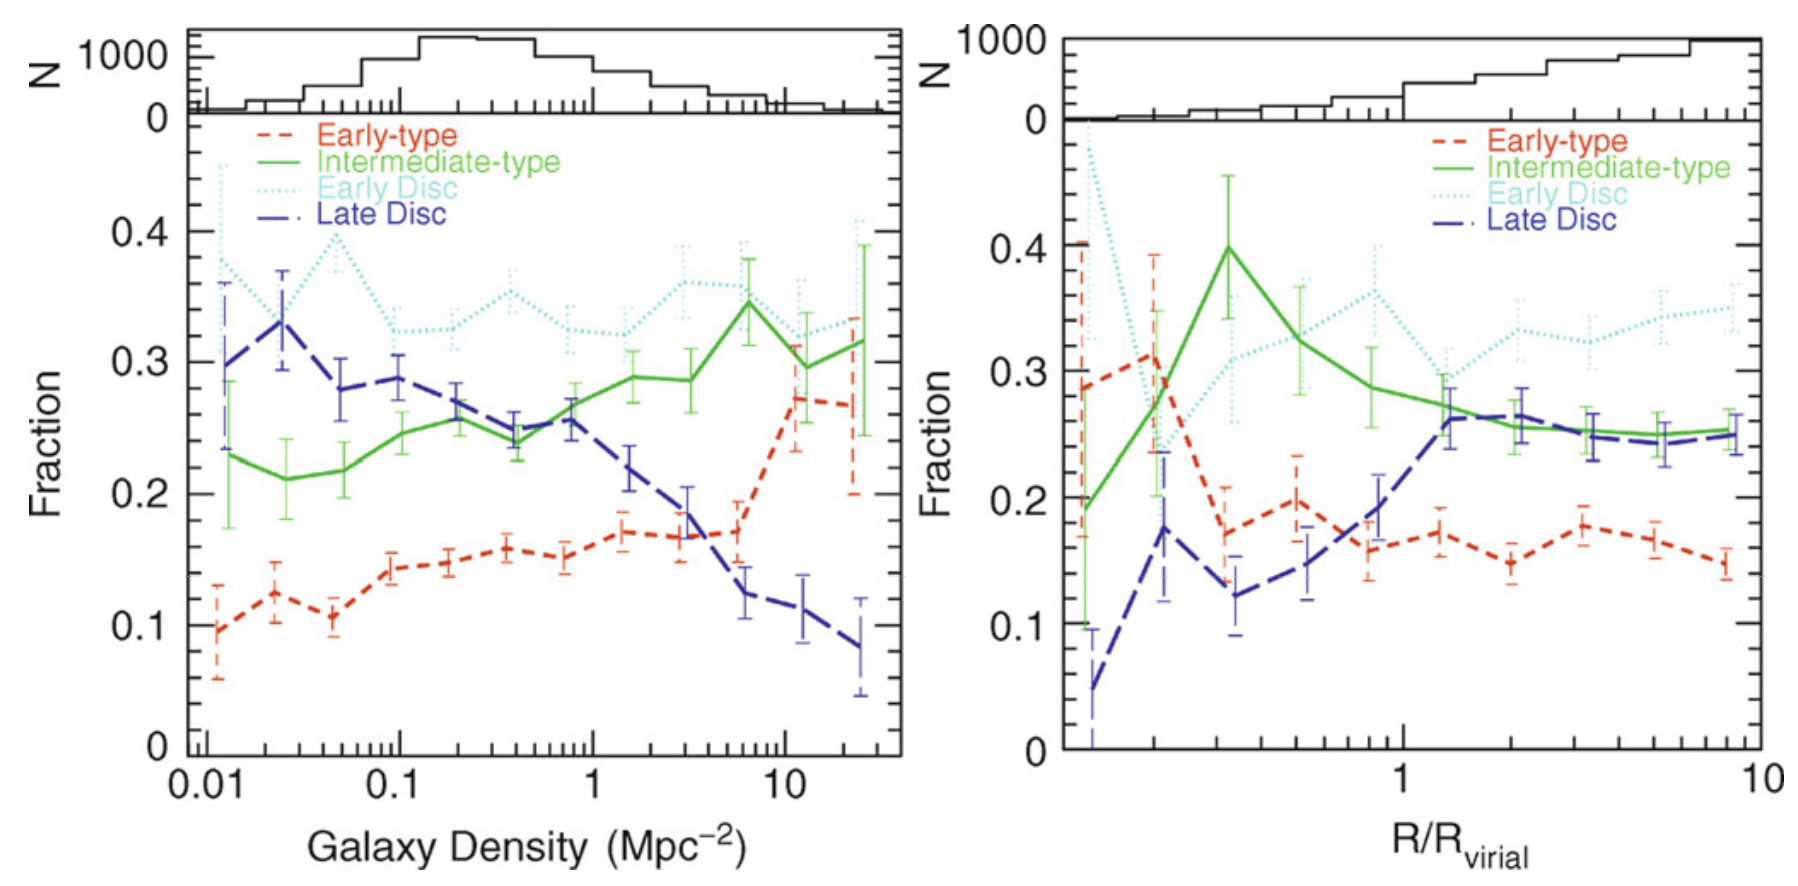
\includegraphics[width=16cm]{figures/extragalactic/DensityMorphology.png}
    \centering
    \caption{\footnotesize{The number fraction of galaxies of different morphologies is plotted as a function of the local galaxy density (left panel), and for galaxies in clusters as a function of the distance from the cluster center, scaled by the corresponding virial radius (right panel). Galaxies are divided into four different classes. `Early-types' contain mainly ellipticals, `intermediates' are mainly S0 galaxies, `early and late discs' are predominantly Sa and Sc spirals, respectively. In both representations, a clear dependence of the galaxy mix on the density or on the distance from the cluster center, respectively, is visible. In the histograms at the top of each panel, the number of galaxies in the various bins is plotted. Source: T. Goto et al. 2003, The morphology-density relation in the Sloan Digital Sky Survey, MNRAS 346, 601, p. 607, 608, Figs. 12, 15. Figure taken from Schneider (2006).}}
    \label{fig:densitymorphology}
\end{figure}

{\noindent}In the right-hand panel of Figure \ref{fig:densitymorphology}, the mixture of galaxy morphologies is plotted as a function of the distance to the center of the nearest cluster, where the distance is scaled by the virial radius of the corresponding cluster. As expected, a very strong dependence of the fraction of ellipticals and spirals on this distance is seen. Sc spirals contribute a mere 5\% of galaxies in the vicinity of cluster centers, whereas the fraction of ellipticals and S0-galaxies strongly increases inwards.

{\noindent}The two diagrams in Figure \ref{fig:densitymorphology} are of course not mutually independent: a region of high galaxy density is very likely to be located in the vicinity of a cluster center, and the opposite is valid accordingly. Therefore, it is not immediately clear whether the mix of galaxy morphologies depends primarily on the respective density of the environment of the galaxies, or whether it is caused by morphological transformations in the inner regions of galaxy clusters.

{\noindent}The density-morphology relation is also seen in galaxy groups. The fraction of late-type galaxies decreases, and the fraction of early-type galaxies increases with decreasing distance from the group center, as is also the case in clusters. When considering the morphological mix of visually classified early- and late-type galaxies, averaged over the whole group or cluster (i.e., up to the virial radius) then it seems to be constant for group/cluster halo masses in excess of $\sim10^{13}\,{\rm M_\odot}$.

{\noindent}A closer examination of Figure \ref{fig:densitymorphology} may provide a clue as to what physical processes are responsible for the dependence of the morphological mix on the local number density. We consider first the right-hand panel of Figure \ref{fig:densitymorphology}. Three different regimes in radius can be identified: for $R\gtrsim R_\mathrm{vir}$, the fraction of the different galaxy types remains basically constant. In the intermediate regime, $0.3\gtrsim R/R_\mathrm{vir}\gtrsim1$, the fraction of S0 galaxies strongly increases inwards, whereas the fraction of late-type spirals decreases accordingly. This result is compatible with the interpretation that in the outer regions of galaxy clusters spirals lose gas, for instance by their motion through the intergalactic medium (IGM), and these galaxies then transform into passive S0 galaxies. Below $R\lesssim0.3\,R_\mathrm{vir}$, the fraction of S0 galaxies decreases strongly, and the fraction of ellipticals increases substantially.

{\noindent}In fact, the ratio of the number densities of S0 galaxies and ellipticals, for $R\lesssim0.3\,R_\mathrm{vir}$, strongly decreases as $R$ decreases. This may hint at a morphological transformation in which S0 galaxies are turned into ellipticals, probably by collisions or mergers. Such gas-free mergers, also called `dry mergers', may be the preferred explanation for the generation of elliptical galaxies. One of the essential properties of dry mergers is that such a merging process would not be accompanied by a burst of star formation, unlike the case of gas-rich collisions of galaxies. The existence of a population of newly born stars in ellipticals would be difficult to reconcile with the generally old stellar population actually observed in these galaxies.

{\noindent}Considering now the dependence on local galaxy density (the left-hand panel of Figure \ref{fig:densitymorphology}), a similar behavior of the morphological mix of galaxies is observed: there seems to exist two characteristic values for the galaxy density where the relative fractions of galaxy morphologies change noticeably. Interestingly, the relation between morphology and density seems to evolve only marginally between $z=0.5$ and the local Universe.

{\noindent}One clue as to the origin of the morphological transformation of galaxies in clusters, as a function of distance from the cluster center, comes from the observation that the velocity dispersion of very bright cluster galaxies seems to be significantly smaller than that of less luminous ones. Assuming that the mass-to-light ratio does not vary substantially among cluster members, this then indicates that the most massive galaxies have smaller velocity dispersions. One way to achieve this trend in the course of cluster evolution is by dynamical interactions between cluster galaxies. Such interactions tend to `thermalize' the velocity distribution of galaxies, so that the mean kinetic energy of galaxies tends to become similar. This then causes more massive galaxies to become slower on average. If this interpretation holds, then the morphology-density relation may be attributed to these dynamical interactions, rather than to the (so-called ram-pressure) stripping of the ISM as the galaxies move through the ICM. However, ram-pressure stripping of the ISM has been clearly observed in clusters. This effect mostly acts on the atomic gas of spirals, whereas the molecular gas seems to be less affected; we recall that the molecular gas is more densely concentrated towards the galactic disk, and thus more strongly bound. In fact, it has been known for a long time that there are spiral galaxies in groups and clusters which are deficient in neutral hydrogen, relative to field galaxies of the same stellar luminosity. If ram-pressure stripping, or other effects in the dense cluster environment, removes the ISM from spirals, then the result could be a disk galaxy without ongoing star formation -- something that may resemble an S0 galaxy. If that were the case, than S0s would be passively fading former spirals. Whereas the original spirals satisfied the Tully-Fisher relation, the S0s would then be expected to be considerably fainter than spirals, at fixed rotational velocity; this indeed is the case.

\subsubsection{Follow-up Questions}

\begin{itemize}
    \item What processes in a cluster convert galaxies?
    \item Where is galaxy harassment most effective (due to relative speeds)?
\end{itemize}


% --------------------------------------------------------------
%               8. 
% --------------------------------------------------------------

\newpage
\subsection{Question 8}

Draw the spectral energy distribution (SED) of a galaxy formed by a single burst of star formation at the ages of $10\,\mathrm{Myrs}$, $2\,\mathrm{Gyrs}$, and $10\,\mathrm{Gyr}$. Please highlight the change over time in the $4000$ Angstrom break.

\subsubsection{Short answer}

Answer.

\subsubsection{Additional context}

{\noindent}The light of normal galaxies originates from stars. Stellar evolution is largely understood, and the spectral radiation of stars can be calculated from the theory of stellar atmospheres. If the distribution of the number density of stars is known as a function of their mass, chemical composition, and evolutionary stage, we can compute the light emitted by them. The theory of population synthesis aims at interpreting the spectrum of galaxies as a superposition of stellar spectra. We have to take into account the fact that the distribution of stars changes over time; e.g., massive stars leave the main sequence after several $10^6\,{\rm yr}$, the number of luminous blue stars thus decreases, which means that the spectral distribution of the population also changes in time. The spectral energy distribution (SED) of a galaxy thus reflects its history of star formation (SF) and stellar evolution. For this reason, simulating different SF histories and comparing them with observed galaxy spectra provides important clues for understanding the evolution of galaxies. Let's discuss some aspects of the theory of population synthesis; this subject is of tremendous importance for our understanding of galaxy spectra.

{\noindent}The processes of SF are not understood in detail; for instance, it is currently impossible to compute the mass spectrum of a group of stars that jointly formed in a molecular cloud. Obviously, high-mass and low-mass stars are born together and form young (open) star clusters. The mass spectra of these stars are determined empirically from observations.

{\noindent}The initial mass function (IMF) is defined as the initial mass distribution at the time of birth of the stars, such that $\xi(m)\mathrm{d}m$ specifies the fraction of stars in the mass interval of width $\mathrm{d}m$ around $m$, where the distribution is normalized,

\begin{align*}
    \int\limits_{m_L}^{m_U} m\xi(m)\,\mathrm{d}m = 1\,{\rm M}_\odot.
\end{align*}

{\noindent}The integration limits are not well defined. Typically, one uses $m_L=0.1\,{\rm M_\odot}$ because stars less massive than $\approx0.08\,{\rm M_\odot}$ do not ignite their hydrogen (and are thus brown dwarfs), and $m_U\sim100\,{\rm M_\odot}$ because considerably more massive stars are not observed. Whereas such very massive stars would in any case be difficult to observe because of their very short lifetime, the theory of stellar structure tells us that more massive stars can probably not form a stable configuration due to excessive radiation pressure. The shape of the IMF is also subject to uncertainties; in most cases, the Salpeter-IMF is used,

\begin{align*}
    \xi(m) \propto m^{-2.35} ~ [{\rm units???}],
\end{align*}

{\noindent}as obtained from investigating the stellar mass spectrum in young star clusters. It is by no means clear whether a universal IMF exists, or whether it depends on specific conditions like metallicity, the mass of the galaxy, cosmic epoch, or other parameters. Given the difficulties of determining the shape of the IMF, apparent variations of the IMF with epoch or environment may be attributed to other effect, such as the specifics of the star-formation history in galaxies. Therefore, there seems to be no clear direct indication that the IMF varies with environment. However, some properties of high-redshift galaxies are very difficult to understand if their IMF was the same as in our neighborhood. It has therefore been suggested that the IMF in starbursts is different from that of quiescent star formation such as we are experiencing in the Milky Way.

{\noindent}The Salpeter-IMF seems to be a good description for stars with $M\gtrsim1\,{\rm M_\odot}$, whereas the IMF for less massive stars is flatter. Note that, due to the steep slope of the IMF, most of the stellar mass is contained in low-mass stars. However, since the luminosity of main-sequence stars depends strongly on mass, approximately as $L\propto M^3$, most of the luminosity comes from high-mass stars.

{\noindent}The star-formation rate (SFR) is the gas mass that is converted into stars per unit time,

\begin{align*}
    \mathrm{SFR} = -\frac{\mathrm{d}M_\mathrm{gas}}{\mathrm{d}t} ~ [{\rm M_\odot\,yr^{-1}}].
\end{align*}

{\noindent}The metallicity $Z$ of the ISM defines the metallicity of the newborn stars, and the stellar properties in turn depend on $Z$. During stellar evolution, metal-enriched matter is ejected into the ISM by stellar winds, planetary nebulae, and SNe, so that $Z(t)$ is an increasing function of time. This chemical enrichment must be taken into account in population synthesis studies in a self-consistent form.

{\noindent}Let $S_{\lambda,Z}(t')$ be the emitted energy per wavelength and time interval, normalized to an initial total mass of $1\,{\rm M_\odot}$, emitted by a group of stars of initial metallicity $Z$ and age $t_0$. The function $S_{\lambda,Z(t-t_0)}(t')$, which describes this emission at any point $t$ in time, accounts for the different evolutionary tracks of the stars in the (HRD). It also accounts for their initial metallicity (i.e., at time $t-t'$), where the latter follows from the chemical evolution of the ISM of the corresponding galaxy. Then the total spectral luminosity of this galaxy at a time $t$ is given by

\begin{align*}
    F_\lambda(t) = \int\limits_0^t \mathrm{SFR}(t-t')S_{\lambda,Z(t-t')}(t')\,\mathrm{d}t' ~ [{\rm erg\,s^{-1}\,cm^{-2}\,Hz^{-1}}],
\end{align*}

{\noindent}thus by the convolution of the star formation rate with the spectral energy distribution of the stellar population. In particular, $F_\lambda(t)$ depends on the star formation history.

\begin{figure}[t]
    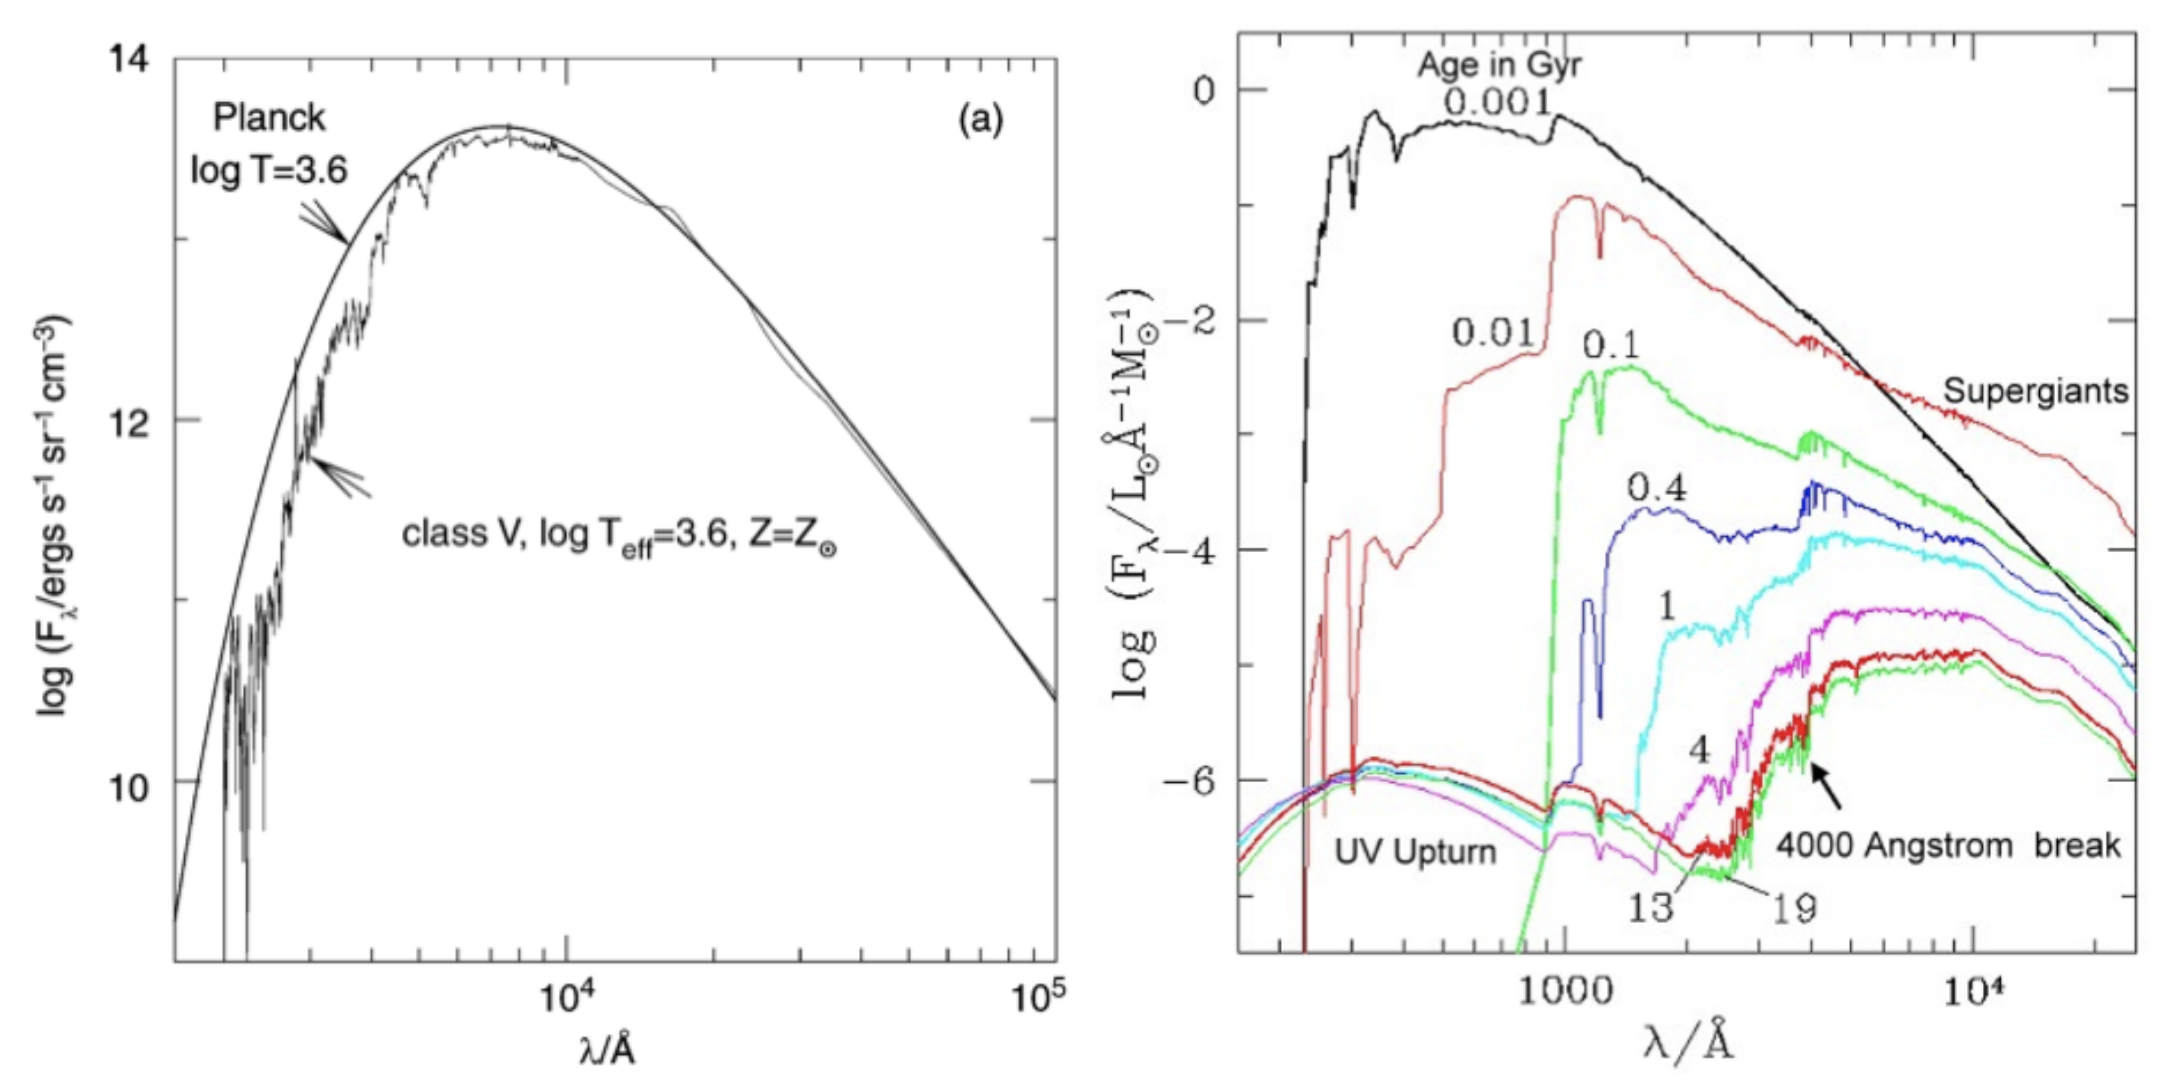
\includegraphics[width=16cm]{figures/extragalactic/SED_SF.png}
    \centering
    \caption{\footnotesize{(a) Comparison of the spectrum of a MS star with a black body spectrum of equal effective temperature. The opacity of the stellar atmosphere causes clear deviations from the Planck spectrum in the UV/optical. (b) Spectrum of a stellar population with Solar metallicity that was instantaneously born a time $t$ ago; t is given in units of $10^9\,{\rm yr}$. Source: S. Charlot 1996, Spectral Evolution of Galaxies, Lecture Notes in Physics 470, Springer-Verlag, p. 53. Figure taken from Schneider (2006).}}
    \label{fig:sedsf}
\end{figure}

\begin{figure}[t]
    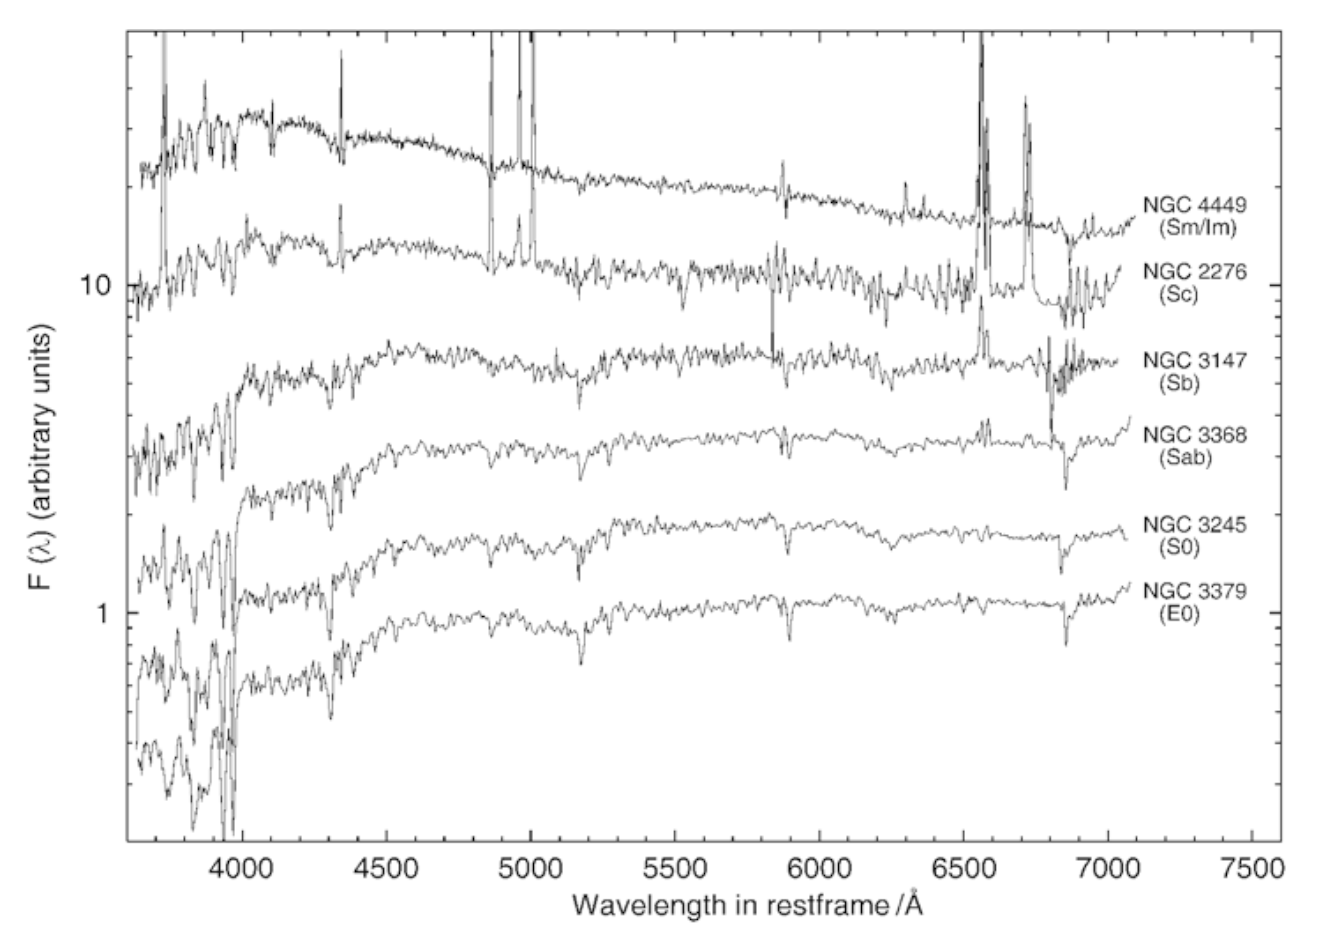
\includegraphics[width=16cm]{figures/extragalactic/StellarSpectra.png}
    \centering
    \caption{\footnotesize{Spectra of galaxies of different types, where the spectral flux is plotted logarithmically in arbitrary units. The spectra are ordered according to the Hubble sequence, with early types at the bottom and late-type spectra at the top. Data from R. Kennicutt 1992, ApJS 79, 255. Figure taken from Schneider (2006).}}
    \label{fig:stellarspectra}
\end{figure}

{\noindent}In the beginning, the spectrum and luminosity of a stellar population are dominated by the most massive stars, which emit intense UV radiation. But after $\sim10^7\,{\rm yr}$, the flux below $1,000$\,\AA is diminished significantly, and after $\sim10^8\,{\rm yr}$, it hardly exists any more. At the same time, the flux in the NIR increases because the massive stars evolve into red supergiants.

{\noindent}For $10^8\,{\rm yr}\gtrsim t\gtrsim10^9\,{\rm yr}$, the emission in the NIR remains high, whereas short-wavelength radiation is more and more diminished. After $\sim10^9\,{\rm yr}$, red giant stars (RGB stars) account for most of the NIR production. After $\sim3\times10^9\,{\rm yr}$, the UV radiation increases again slightly, due to blue stars on the horizontal branch into which stars evolve after the AGB phase, and due to white dwarfs which are hot when they are born. Between an age of $4$ and $13$ billion years, the spectrum of a stellar population evolves fairly little. 

{\noindent}Of particular importance is the spectral break located at about $4,000$\,\AA which becomes visible in the spectrum after a few $10^7\,{\rm yr}$. This break is caused by a strongly changing opacity of stellar atmospheres at this wavelength, mainly due to strong transitions of singly ionized calcium and the Balmer lines of hydrogen. This $4,000$\,\AA break is one of the most important spectral properties of the continuum stellar emission in galaxies; it allows us to estimate the redshifts of early-type galaxies from their photometric properties -- so-called photometric redshift estimates.

\subsubsection{Follow-up Questions}

\begin{itemize}
    \item Why do we only consider a single burst of SF? (Want to hear about population synthesis.)
    \item If you looked at an actual SED, what else would you see besides the mostly smooth continuum and spectral breaks?
    \item What's a typical emission line you would see in the optical part of the spectrum?
    \item Why is the y-axis is $\lambda\mathrm{F}_\lambda$, what does that mean?
\end{itemize}


% --------------------------------------------------------------
%               9. 
% --------------------------------------------------------------

\newpage
\subsection{Question 9}

How are galaxy redshifts estimated by photometric techniques?

\subsubsection{Short answer}

Answer.

\subsubsection{Additional context}

The Lyman-break technique is a special case of a method for estimating the redshift of galaxies (and QSOs) by multi-color photometry. This technique can be employed due to the spectral breaks at $912\,$\AA and $1216\,$\AA, respectively. Spectra of galaxies also show other characteristic features. The broadband energy distribution is basically a superposition of stellar radiation (if we ignore for a moment the presence of dust, which can yield a substantial infrared emission from galaxies). A stellar population of age $\gtrsim10^8\,{\rm yr}$ features a $4,000\,$\AA break because, due to a sudden change in the opacity at this wavelength, the spectra of most stars show such a break at about $4,000\,$\AÅ (see Figure \ref{fig:sedsf}). Hence, the radiation from a stellar population at $<4,000\,$\AÅ is less intense than at $>4,000\,$\AA; this is the case particularly for early-type galaxies, as can be seen in Figure \ref{fig:stellarspectra}, due to their old stellar population.

{\noindent}If we assume that the star-formation histories of galaxies are not too diversified, the spectral energy distributions of these galaxies are expected to follow certain patterns. For example, if all galaxies had a single episode of star formation, starting at their formation redshift $z_f$ and lasting for a time $t$, then the spectra of these galaxies, for a given initial mass function, would be characterized by these two parameters, as well as the total stellar mass formed; this latter quantity then yields the amplitude of the spectrum, but does not affect the spectral shape. When measuring the magnitude of these galaxies in $n$ broad-band filters, we can form $n-1$ independent colors. Next suppose we form a multidimensional CCD, in which every galaxy is represented by a point in this ($n-1$)-dimensional color space. Considering only galaxies at the present epoch, all these points will lie on a two-dimensional surface in this multi-dimensional space, instead of being more or less randomly distributed.

{\noindent}Next, instead of plotting $z=0$ galaxies, we consider the distribution of galaxies at some higher redshift $z<z_f$. This distribution of points will be different, mainly due to two different effects. First, a given photometric filter corresponds to a different rest-frame spectral range of the galaxy, due to redshift. Second, the ages of the stellar populations are younger at an earlier cosmic epoch, and thus the spectral energy distributions are different. Both of these effects will cause these redshift $z$ galaxies to occupy a different two-dimensional surface in multi-color space.

{\noindent}Generalizing this argument further, we see that in this idealized consideration, galaxies will occupy a three-dimensional subspace in ($n-1$)-dimensional color space, parametrized by formation redshift $z_f$, time-scale $t$, and the galaxy’s redshift $z$. Hence, from the measurement of the broad-band energy distribution of a galaxy, we might expect to be able to determine, or at least estimate, its redshift, as well as other properties such as the age of its stellar population; this is the principle of the method of photometric redshifts.

\begin{figure}[h]
    \floatbox[{\capbeside\thisfloatsetup{capbesideposition={right,top},capbesidewidth=4cm}}]{figure}[\FBwidth]
    {\caption{\footnotesize{The bottom panel illustrates again the principle of the drop-out method, for a galaxy at $z\sim3.2$. Whereas the Lyman-$\alpha$ forest absorbs part of the spectral flux between (rest-frame wavelength) $912$ and $1216$\,\AA, the flux below $912\,$\AA vanishes almost completely. By using different combinations of filters (top panel), an efficient selection of galaxies at other redshifts is also possible. The example shows a galaxy at $z=1$ whose $4,000\,$\AA break is located between the two redder filters. The $4,000\,$\AA break occurs in stellar populations after several $10^7\,{\rm yr}$ (see Figure \ref{fig:sedsf}) and is one of the most important features for the method of photometric redshift. Source: K.L. Adelberger 1999, Star Formation and Structure Formation at Redshifts $1<z<4$, astro-ph/9912153, Fig. 1. Figure taken from Schneider (2006).}}
    \label{fig:photredshifts}}
    {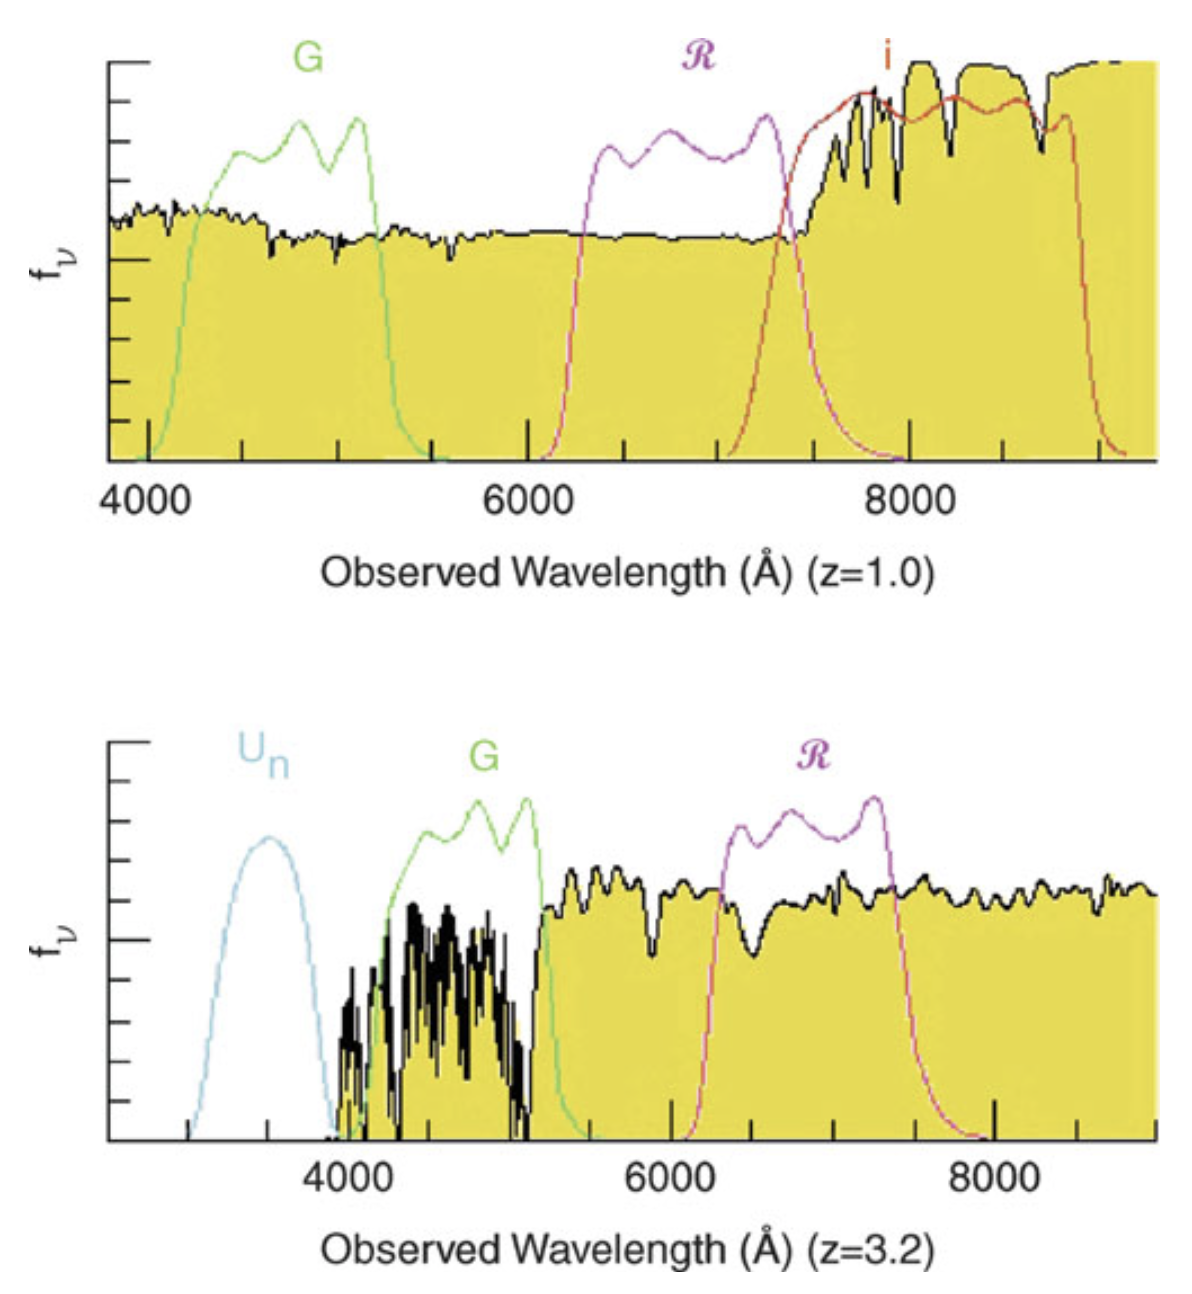
\includegraphics[width=12cm]{figures/extragalactic/PhotRedshifts.png}}
\end{figure}

{\noindent}Of course, the situation is considerably more complicated in reality. Galaxies most likely have a more complicated SF history than assumed here, and hence they will not be confined to a two-dimensional surface at fixed redshift, but instead will be spread around this surface. The spectrum of a stellar population also depends on its metallicity, as well as absorption, either by gas and dust in the ISM or hydrogen in intergalactic space (of which the Lyman-break method makes proper use). On the other hand, the colors of current-day galaxies are remarkably similar, best indicated by the red sequence. Therefore, the method of photometric redshifts may be expected to work, even if more complications are accounted for than in the idealized example considered above.

{\noindent}The method is strongly aided if the galaxies have characteristic spectral features, which shift in wavelength as the redshift is changed. If, for example, the spectrum of a galaxy was a power law in wavelength, then the redshifted spectrum would as well be a power law, with the same spectral slope -- if we ignore the different age of the stellar population. Therefore, for such an SED is would be impossible to estimate a redshift. However, if the spectrum shows a clear spectral break, then the location of this break in wavelength depends directly on the redshift, thus yielding a particularly clean diagnostic. In this context the $4,000\,$\AA break and the Ly$\alpha$-break play a central role, as is illustrated in Figure \ref{fig:photredshifts}.

{\noindent}In order to apply this method, one needs to find the characteristic domains in color space where (most of) the galaxies are situated. This can be done either empirically, using observed SEDs of galaxies, or by employing population synthesis models. More precisely, a number of standard spectra of galaxies (so-called templates) are used, which are either selected from observed galaxies or computed by population synthesis models. Each of these template spectra can then be redshifted in wavelength. For each template spectrum and any redshift, the expected galaxy colors are determined by integrating the spectral energy distribution, multiplied by the transmission functions of the applied filters, over wavelength. This set of colors can then be compared with the observed colors of galaxies, and the set best resembling the observation is taken as an estimate for not only the redshift but also the galaxy type.

{\noindent}The advantage of this method is that multi-color photometry is much less time-consuming than spectroscopy of galaxies. Whereas some modern spectrographs allow one to take spectra of $\sim1,000$ objects simultaneously, images taken with wide-field cameras of $1\,\mathrm{deg}^2$ on $4\,{\rm m}$ class telescopes record the fluxes of $10^5$ galaxies in a one hour exposure. In addition, this method can be extended to much fainter magnitudes than are achievable for spectroscopic redshifts. The disadvantage of the method becomes obvious when an insufficient number of photometric bands are available, since then the photometric redshift estimates can yield a completely wrong $z$; these are often called catastrophic outliers. One example for the occurrence of extremely wrong redshift estimates is provided by a break in the spectral energy distribution. Depending of whether this break is identified as the Lyman-break or the $4,000\,$\AA break, the resulting redshift estimates will be very different. To break the corresponding degeneracy, a sufficiently large number of filters spread over a broad spectral range must be available to probe the spectral energy distribution over a wide range in wavelengths. As a general rule, the more photometric bands are available and the smaller the uncertainties in the measured magnitudes, the more accurate the estimated redshift. Normally, data from four or five photometric bands are required to obtain useful redshift estimates. In particular, the reliability of the photometric redshift benefits from data over a large wavelength range, so that a combination of several optical and NIR filters is desirable.

{\noindent}The successful application of this method also depends on the type of the galaxies. Early-type galaxies form a relatively well-defined color-magnitude sequence at any redshift, due to their old stellar populations (manifested in clusters of galaxies in form of the red cluster sequence), so that the redshift of this type of galaxy can be estimated very accurately from multi-color information. However, this is only the case if the $4,000\,$\AA break is located in between two of the applied filters. For $z\sim1$ this is no longer the case if only optical filters are used. Other types of galaxies show larger variations in their spectral energy distribution, depending, e.g., on the star formation history, as mentioned before.

{\noindent}Photometric redshifts are particularly useful for statistical purposes, for instance in situations in which the exact redshift of each individual galaxy in a sample is of little relevance. However, by using a sufficient number of optical and NIR filters, quite accurate redshift estimates for individual galaxies are achievable. For example, with eight optical and NIR bands and accurate photometry, a redshift accuracy of  $\Delta z\sim0.03(1+z)$ was obtained, as demonstrated in Figure \ref{fig:photvsspecredshift} by a comparison of photometric redshifts with redshifts determined spectroscopically for galaxies in the field of the HDF-North. If data in additional photometric bands are available, e.g., using filters of smaller transmission curves (`intermediate width filters'), the redshift accuracy can be increased even more, e.g., $\Delta z\sim0.01(1+z)$ was obtained using a total of 30 photometric bands.

\begin{figure}[t]
    \floatbox[{\capbeside\thisfloatsetup{capbesideposition={right,top},capbesidewidth=4cm}}]{figure}[\FBwidth]
    {\caption{\footnotesize{Photometric redshift versus the spectroscopic redshift for galaxies in the HDF-North. Photometric data in four optical and two NIR bands have been used here. We see how accurate photometric redshifts can be -- their quality depends on the photometric accuracy in the individual filters, the number of filters used, the redshift and the type of the galaxy, and also on details of the applied analysis method. Source: N. Benítez 2000, Bayesian Photometric Redshift Estimation, ApJ 536, 571, p. 579, Fig. 5. Figure taken from Schneider (2006).}}
    \label{fig:photvsspecredshift}}
    {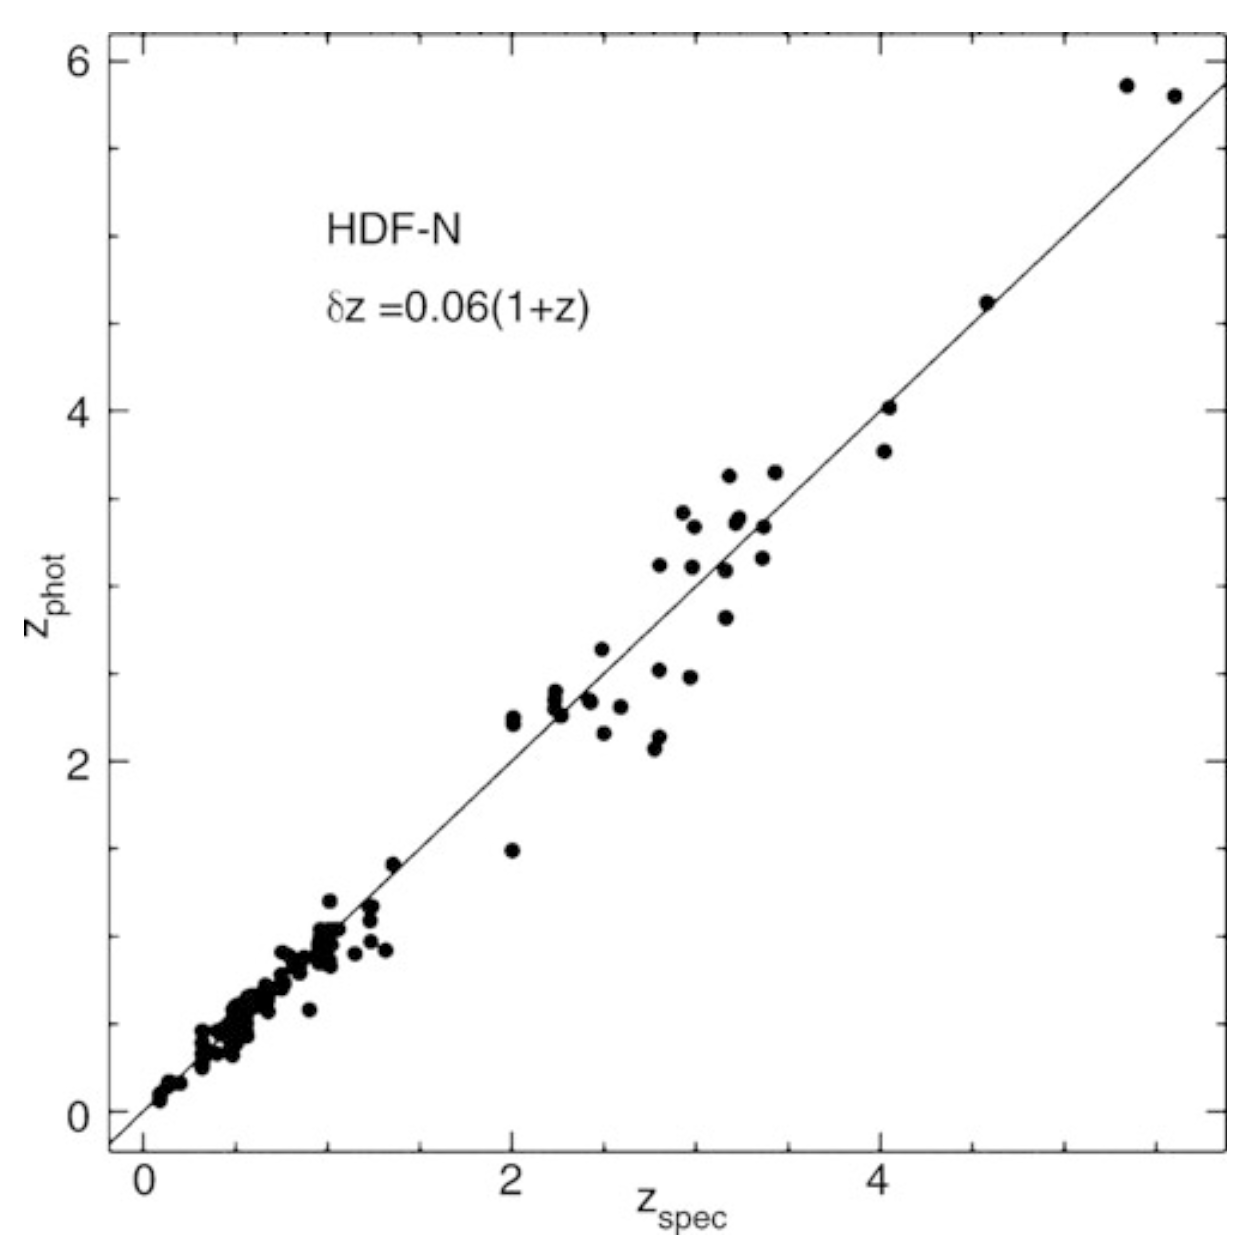
\includegraphics[width=10cm]{figures/extragalactic/PhotVsSpecRedshift.png}}
\end{figure}

\subsubsection{Follow-up Questions}

\begin{itemize}
    \item What problems are there with the photometric method?
    \item How do you account for different galaxy types, and what do you need to know about the stellar population? (i.e., IMF.)
\end{itemize}


% --------------------------------------------------------------
%               10. 
% --------------------------------------------------------------

\newpage
\subsection{Question 10}

Draw a spectrum of a high-redshift quasar. What do quasar emission lines typically look like? Explain what we see in the spectrum at rest wavelengths bluer than $1216$ Angstroms.

\subsubsection{Short answer}

Answer.

\subsubsection{Additional context}

{\noindent}The first quasars (for `quasi-stellar radio source') were discovered  as `radio galaxies with no galaxy'. They appeared point-like in optical photographs; only their enormous redshifts betrayed that they were not Galactic stars. Rather, they were gigaparsecs distant, and hence extremely luminous. Subsequently `radio-quiet' quasars, called quasi-stellar objects, or QSOs, were found by searching for objects that appeared stellar, but emitted too strongly at infrared or ultraviolet wavelengths relative to their brightness in visible light. Radio-quiet QSOs outnumber radio-loud quasars by at least a factor of 30; both are now believed to be variants of the same type of object, so we use the term `quasar' to include the QSOs. In the 1980s, deep images of nearby quasars showed us that they were in fact the bright nuclei of galaxies, so luminous as to outshine the surrounding stars. Most astronomers now regard quasars as more powerful versions of a Seyfert nucleus. Quasars cover a very wide range in luminosity; the most powerful are also the rarest.

{\noindent}Quasars are the most luminous members of the class of AGNs. The optical and ultraviolet spectrum of a quasar typically shows strong broad emission lines characteristic of moderately dense gas (Figure \ref{fig:qsoradioquiet}). The widths of the lines correspond to the Doppler shifts expected from emitting gas travelling at speeds $\sim10,000\,{\rm km\,s^{-1}}$. These emitting clouds are moving much faster than the galaxy's stars, which typically orbit at a few hundred kilometers per second. Many AGN are variable, changing their luminosity substantially within a few months, days, or even hours. The emission lines also strengthen and decline, within a few days or weeks. To allow such fast variability, both broad lines and continuum radiation must come from a region no more than a few light-weeks across.

\begin{figure}[h]
    \centering
    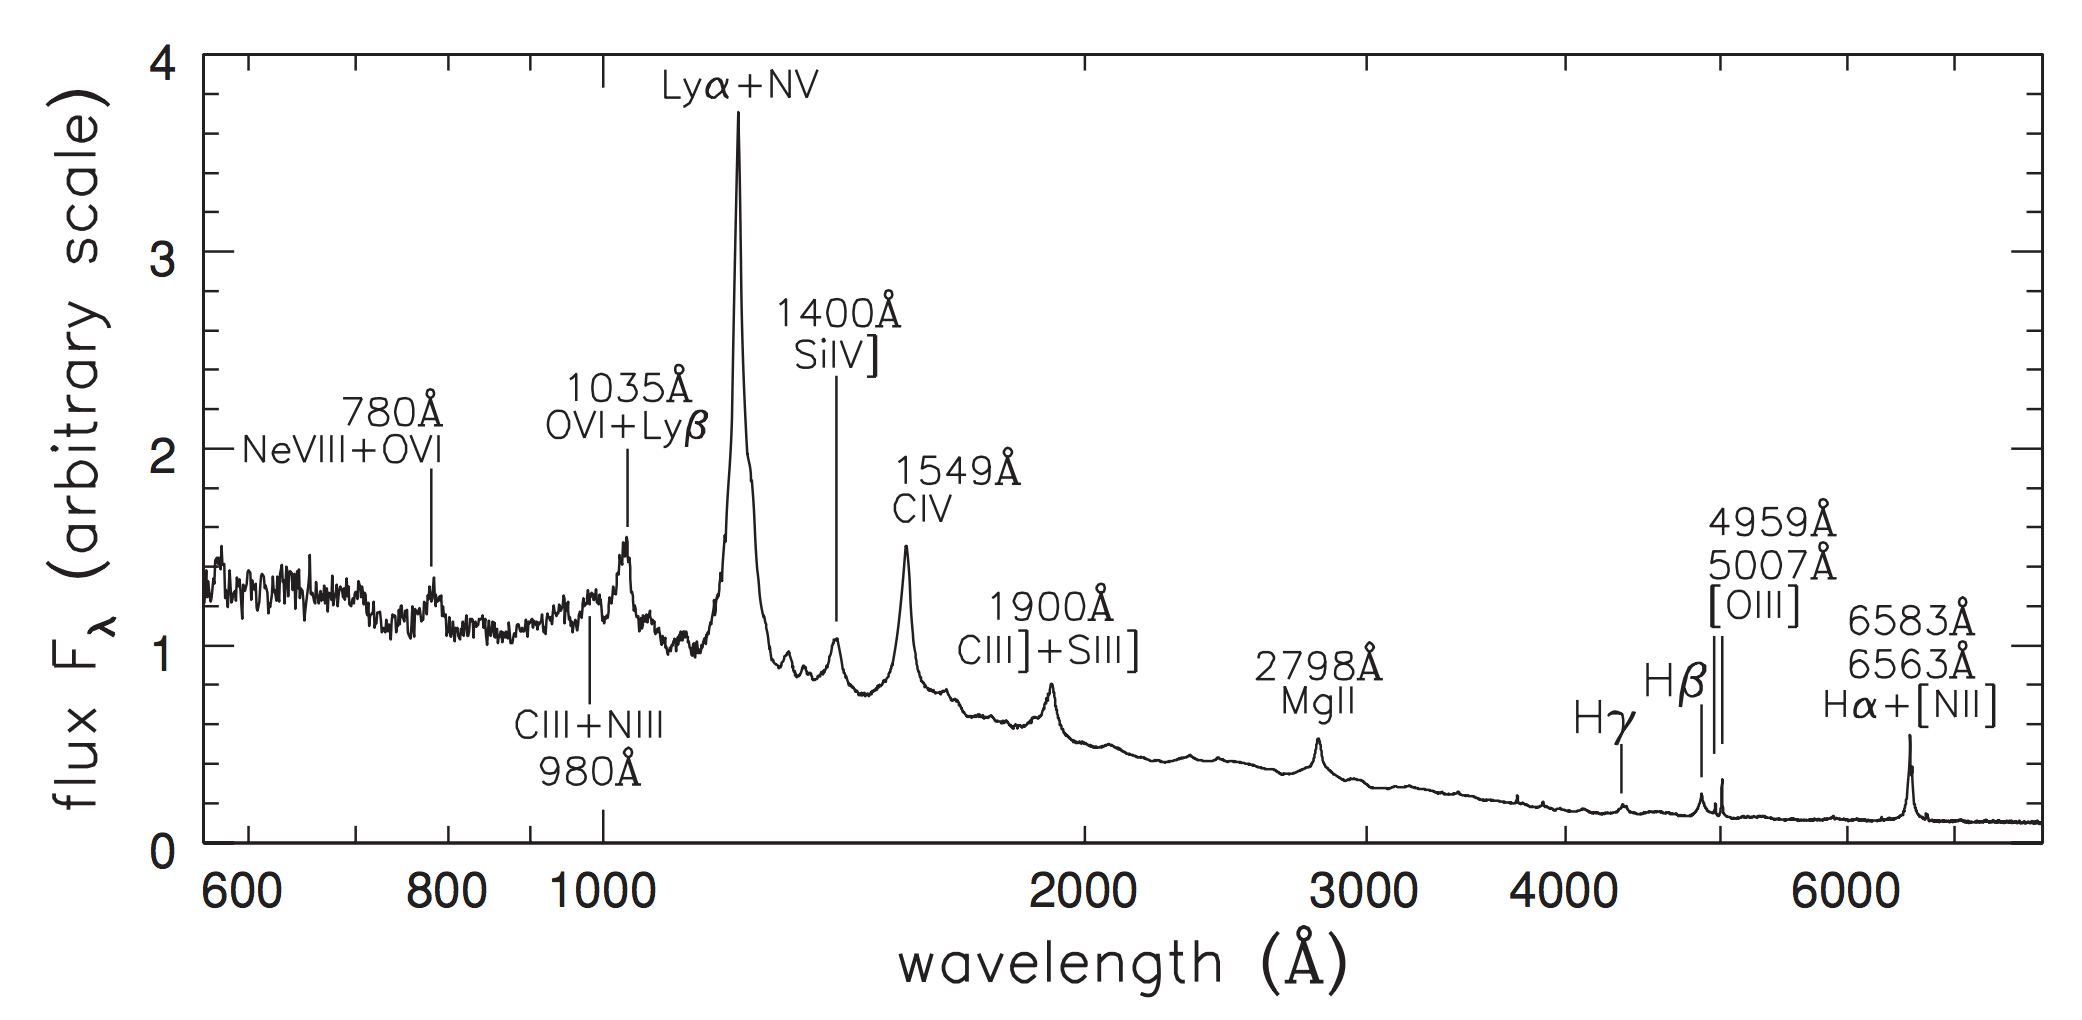
\includegraphics[width=16cm]{figures/extragalactic/QSO_radioquiet.png}
    \caption{\footnotesize{The ultraviolet and optical spectrum of an `average' radio-quiet quasar. Source: R.Telfer et al. 2002 Ap J 565, 773. Figure taken from Sparke \& Gallagher (2007).}}
    \label{fig:qsoradioquiet}
\end{figure}

{\noindent}Interestingly, the flux of the source varies at nearly all frequencies, where the variability time-scale differs among the objects and also depends on the wavelength. As a rule, it is found that the variability time-scale of the observed radiation is smaller, and its amplitude larger, at higher frequencies. The optical spectrum is very blue; most quasars at redshifts $z\lesssim2$ have $(U-B)<-0.3$ (for comparison, only hot white dwarfs have a similarly blue color index). Besides this blue continuum, very broad emission lines are characteristic of the optical and UV spectrum. Some of them correspond to transitions of very high ionization energy.

{\noindent}The continuum spectrum of a quasar can often be described, over a broad frequency range, by a power law of the form

\begin{align*}
    S_\nu \propto \nu^{-\alpha},
\end{align*}

{\noindent}where $\alpha$ is the spectral index. A spectral index of $\alpha-0$ corresponds to a flat spectrum, whereas $\alpha=1$ describes a spectrum in which the same energy is emitted in every logarithmic frequency interval. Incidentally, the energy distribution seen in Fig \ref{fig:qsoradioquiet} corresponds approximately to the latter case, over more than ten orders of magnitude in frequency, although over smaller frequency ranges, the spectral shape differs markedly from $\alpha=1$.


% --------------------------------------------------------------
%               11. 
% --------------------------------------------------------------

\newpage
\subsection{Question 11}

Sketch the SED from the radio to gamma of extragalactic radiation on large angular scales. Describe the source and emission mechanism for each feature.

\subsubsection{Short answer}

Answer.

\subsubsection{Additional context}

Figure \ref{fig:diffusebackground} shows the spectrum of cosmic background radiation, plotted as $\nu I_\nu$ versus wavelength so that the curve shows the intensity per logarithmic frequency interval. Following the terminology of the CMB, these are called background radiation as well. However, the name should not imply that it is a background radiation of cosmological origin, in the same sense as the CMB. The neutrino background that should be present as a relic from the early epochs of the Universe, in the form of a thermal distribution of all three neutrino families with $T\approx1.9\,{\rm K}$, is likely to remain undiscovered for quite some time due to the very small cross section of these low energy neutrinos.

\begin{figure}[h]
    \floatbox[{\capbeside\thisfloatsetup{capbesideposition={right,top},capbesidewidth=4cm}}]{figure}[\FBwidth]
    {\caption{\footnotesize{Spectrum of cosmic background radiation, plotted as $\nu I_\nu$ versus wavelength so that the curve shows the intensity per logarithmic frequency interval. Besides the CMB, background radiation exists in the radio domain (cosmic radio background, CRB), in the infrared (CIB), in the optical/UV (CUVOB), in the X-ray (CXB), and at gamma-ray energies (CGB). With the exception of the CMB, all of these backgrounds can be understood as a superposition of the emission from discrete sources. Source: M.G. Hauser \& E. Dwek 2001, ARA\&A 39, 249, Fig.1. Figure taken from Schneider (2006).}}
    \label{fig:diffusebackground}}
    {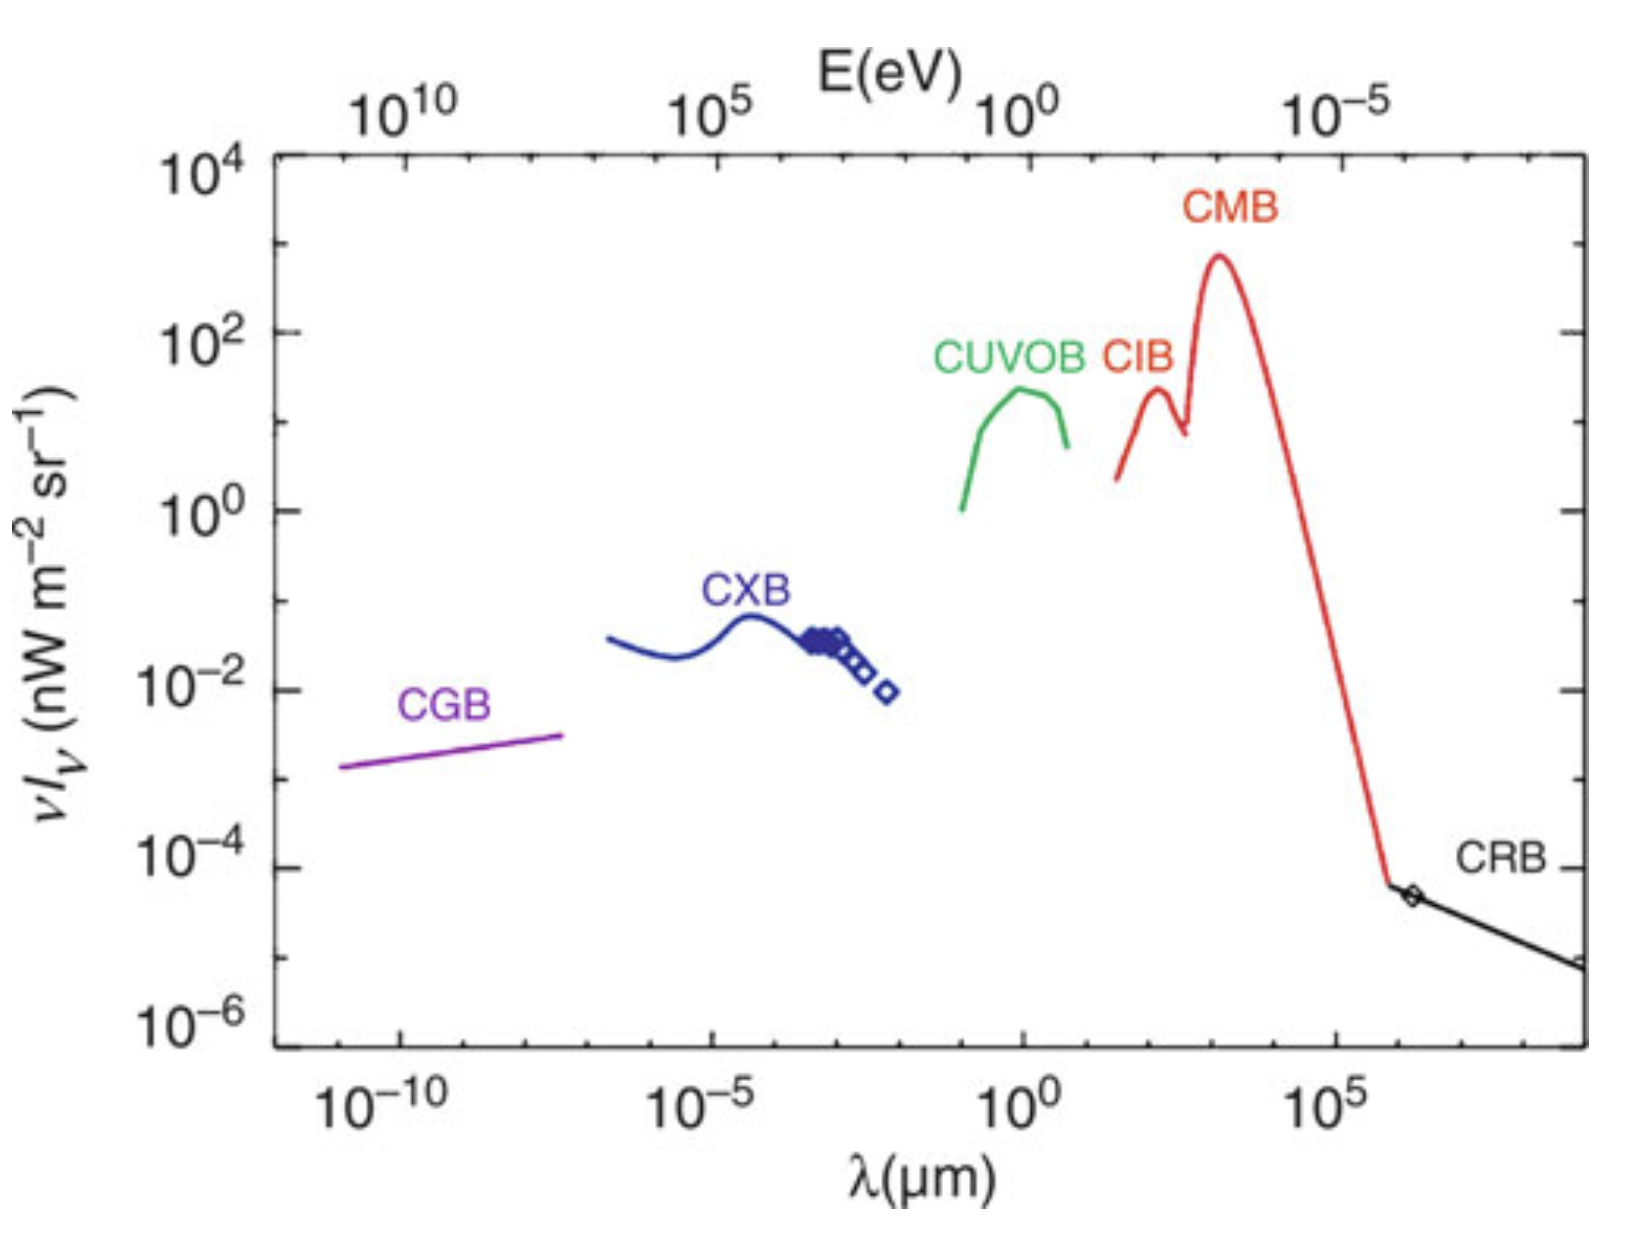
\includegraphics[width=10cm]{figures/extragalactic/DiffuseBackground.png}}
\end{figure}

{\noindent}In the present context, we simply denote the flux in a specific frequency domain, averaged over sky position at high Galactic latitudes, as background radiation. Thus, when talking about e.g., the optical background, we refer to the sum of the radiation of all galaxies and AGNs per solid angle. The interpretation of such a background radiation depends on the sensitivity and the angular resolution of the telescopes used. Imagine, for instance, observing the sky with an optical camera that has an angular resolution of only one arcminute. A relatively isotropic radiation would then be visible at most positions in the sky, featuring only some very bright or very large sources. Thus, the background can be decomposed into a `resolved' component, which can be attributed to individually identified sources, and the unresolved component. On improving the angular resolution, more and more individual sources become visible, so that a larger fraction of the background radiation is resolved. At optical wavebands, the Hubble Deep Fields have resolved essentially all of the background into individual sources. In analogy to this, one may wonder whether the CXB or the CIB can likewise be understood as a superposition of radiation from discrete sources.

{\noindent}\textbf{Cosmic gamma-ray background (CGB)}: 

{\noindent}\textbf{Cosmic x-ray background (CXB)}: The first X-ray experiment in astronomy, a balloon flight in 1962, discovered a diffuse X-ray emission across the sky, confirmed by the first X-ray satellites which discovered not only a number of extragalactic X-ray sources (such as AGNs and clusters of galaxies), but also an apparently isotropic radiation component. The spectrum of the cosmic X-ray background (CXB) is a very hard (i.e., flat) power law, cut off at an energy above $40\,{\rm keV}$, which can roughly be described by

\begin{align*}
    I_\nu \propto E^{-0.3}\exp\left(-\frac{E}{E_0}\right),
\end{align*}

{\noindent}with $E_0\sim40\,{\rm keV}$. 

{\noindent}Initially, the origin of this radiation was unknown, since its spectral shape was different from the spectra of sources that were known at that time. For example, it was not possible to obtain this spectrum by a superposition of the spectra of known AGNs. ROSAT, with its substantially improved angular resolution compared to earlier satellites (such as the Einstein observatory), conducted source counts at much lower fluxes, based on some very deep images. From this, it was shown that at least 80\% of the CXB in the energy range between $0.5$ and $2\,{\rm keV}$ is emitted by discrete sources, of which the majority are AGNs. Hence it is natural to assume that the total CXB at these low X-ray energies originates from discrete sources, and observations by XMM-Newton and Chandra have confirmed this.

{\noindent}However, the X-ray spectrum of normal AGNs is different from that seen by the CXB, namely it is considerably steeper(about $S_\nu\propto\nu^{-S0.7}$). Therefore, if these AGNs contribute the major part of the CXB at low energies, the CXB at higher energies cannot possibly be produced by the same AGNs. Subtracting the spectral energy of the AGNs found by ROSAT from the CXB spectrum, one obtains an even harder spectrum, resembling very closely that of thermal bremsstrahlung. Therefore, it was supposed for a long time that the CXB is, at higher energies, produced by a hot intergalactic gas at temperatures of $k_BT\sim30\,{\rm keV}$. This model was excluded, however, by the precise measurement of the thermal spectrum of the CMB by COBE, showing that the CMB has a perfect blackbody spectrum. If a postulated hot intergalactic gas were able to produce the CXB, it would cause significant deviations of the CMB from the Planck spectrum, namely by the inverse Compton effect (the same effect that causes the SZ effect in clusters of galaxies). Thus, the COBE results clearly ruled out this possibility.

{\noindent}Deep observations with Chandra and XMM (e.g., in the CDFS) have finally resolved most of the CXB also at higher energies. From source counts performed in such fields, more than 75\% of the CXB in the energy range of $2\,{\rm keV}<E<10\,{\rm keV}$ could be resolved into discrete sources. Again, most of these sources are AGNs, but typically with a significantly harder (i.e., flatter) spectrum than the AGNs that are producing the low-energy CXB. Such a flat X-ray spectrum can be produced by photoelectric absorption of an intrinsically steep power law spectrum, where photons closer to the ionization energy are more efficiently absorbed than those at higher energy. According to the classification scheme of AGNs, these are Type 2 AGNs, thus Seyfert 2 galaxies and QSOs with strong intrinsic self-absorption. We should recall that Type 2 QSOs have only been detected by Chandra -- hence, it is no coincidence that the same satellite has also been able to resolve the high-energy CXB.

{\noindent}However, at even higher energies most of the CXB was still unaccounted for -- even the observed Type-2 AGNs could not account for it. It thus seems that there is a population of sources in the Universe which dominate the X-ray emission at high energies, still escape the observations at low X-ray frequencies. These could be heavily obscured AGNs, where only the hard X-rays manage to escape the emitting region. With the X-ray telescope onboard the Swift satellite, a significant number of such heavily obscured AGNs were found. Their estimated number density, together with their spectral energy distribution, make it plausible that they are the missing population of `hidden black holes' responsible for the hard CXB.

{\noindent}\textbf{Cosmic optical/ultraviolet background (CUVOB)}: 

{\noindent}\textbf{Cosmic infrared background (CIB)}: The first point to note from Figure \ref{fig:diffusebackground} is the relatively flat energy distribution between the UV- and the mm-regime. Since both the UV-radiation and the far-IR radiation originate almost entirely from star-formation, the flat energy distribution implies that essentially half of the energetic photons emitted from newly-formed stars are absorbed by dust and reradiated in the FIR. Hence, estimates of the star formation activity from UV-flux alone will on average be biased low by 50\%. Observations of background radiation in the infrared are very difficult to accomplish, in particular due to the thermal radiation from the instruments and the zodiacal light. However, the DIRBE and FIRAS instruments onboard COBE provided a measurement of the CIB. The question now is whether the CIB can be understood as well as being due solely to individual sources.

{\noindent}Since mid- and far-IR observations are only possible from space, finding the answer to that question is challenging. Infrared observatories in space have a rather small aperture which, together with the long wavelength, yields a rather large point-spread function (PSF). This implies that when one observes to low flux limits, where the mean angular separation of sources on the sky becomes comparable to the size of the PSF, these sources can not be separated. This yields a lower flux limit for the detection of individual sources, called the confusion limit. The smaller the telescope, the shallower is the confusion limit reached. For example, the flux limit down to which individual sources could be identified with the Spitzer satellite at $160\,\mu{\rm m}$ corresponds to only 7\% of the CIB at this wavelength. The much larger mirror on the Herschel satellite lowered the confusion limit such that individual sources can be identified which account for about 52\% of the CIB. Going to larger wavelength, the confusion limit is even more severe.

{\noindent}However, one can dig deeper into the source counts with a technique called stacking. Taking the position of sources detected at some smaller wavelength (where the confusion limit is fainter), and adding up the flux in the longer wavelength band around all these positions, one obtains the mean long-wavelength flux of these sources. With this method, one will miss all fainter sources which do not have a detected counterpart in the short-wavelength input catalog, so that wavelength should be selected carefully. Given the characteristic spectrum of FIR-bright sources, one expects that most of the sources radiating in the FIR will have an appreciable flux at $24\,\mu{\rm m}$. Since Spitzer was particularly sensitive at this wavelength, the corresponding source catalog is best for a stacking analysis. Furthermore, if the redshifts of the sources selected at $24\,\mu{\rm m}$ is known, the stacking analysis can be used to determine the redshift distribution of the contributions to the CIB in the FIR. With stacking, the source counts can be followed to about three times lower flux than the confusion limit of individual sources permits.

{\noindent}\textbf{Cosmic microwave background (CMB)}: The cosmic microwave background (CMB) is a remnant of the early hot phase of the Universe, namely thermal radiation from the time before recombination. 

{\noindent}\textbf{Cosmic radio background (CRB)}: 

% --------------------------------------------------------------
%               12. 
% --------------------------------------------------------------

\newpage
\subsection{Question 12}

What are AGNs? Describe different observational classes of them and how they may relate to each other.

\subsubsection{Short answer}

Answer.

\subsubsection{Additional context}

A wide range of objects are subsumed under the name AGN, all of which have in common strong non-thermal emission in the core of a galaxy (host galaxy). It is important to keep in mind that the frequency range in which sources are studied affects the source classification. The classification of AGNs is very confusing at first glance. Different classes refer to different appearances of AGNs but do not necessarily correspond to the physical nature of these sources. Similarly, the properties of the emission of AGNs in different wavebands (such as radio or gamma-rays) can differ most strongly. However, the large variety of appearances of AGNs can be understood, at least to a first approximation, by geometric considerations. The emission of an AGN is not isotropic; the flow of material which causes the energy release near the central black hole occurs in the form of a disk (the accretion disk), which defines a pair of preferred directions (i.e., those perpendicular to the plane in which the disk lies). In the context of unified models, the way an AGN appears to us depends strongly on the angle between this disk axis and the line-of-sight to the source.

{\noindent}In Figure \ref{fig:agn}, this geometric picture of an AGN is sketched. The different green arrows indicate different lines-of-sight to observers, and they are labeled with the characteristic AGN class the corresponding observer will see. In the upper half of the figure, it is assumed that the AGN produces strong jets, whereas in the lower part, weaker jets (or none at all) are assumed.\footnote{As is often the case with these figures, this schematic depicts two very different AGN cases -- one with a radio loud jet and one without. No such AGN can have one jet on one side and not the other!} With this picture in mind, we shall now describe the various types of AGNs. Surrounding the central supermassive black hole is an accretion disk which emits the bulk part of the optical and UV continuum emission. The central region around the accretion disk is the source of most of the X-ray radiation. Gas clouds above and below the accretion disk are responsible for the broad emission lines. In the plane of the disk, a distribution of gas and dust is present, which can absorb radiation from the inner region of the AGN; this obscuring material is sometimes depicted as a torus, though its geometry is probably more complicated. Nevertheless, the appearance of the AGN depends on whether the observer is located near the plane of the disk -- where radiation is partly absorbed by the material in the torus -- or placed in a direction closer to the axis of the disk. This concerns in particular the broad line emission, which may be fully obscured for an observer in the plane of the disk. In contrast, the gas responsible for the narrow emission lines is located at much larger distances from the black hole, so that it cannot be fully hidden by the obscuring torus. 

\begin{figure}[h]
    \floatbox[{\capbeside\thisfloatsetup{capbesideposition={right,top},capbesidewidth=4cm}}]{figure}[\FBwidth]
    {\caption{\footnotesize{Sketch of our current understanding of the unification of AGN types. The accretion disk is surrounded by a thick `torus' containing dust which thus obscures the view to the center of the AGN. When looking from a direction near the plane of the disk, a direct view of the continuum source and the BLR is blocked, whereas it is directly visible from directions closer to the symmetry axis of the disk. The difference between Seyfert 1 (and BLRG) and Seyfert 2 (and NLRG) is therefore merely a matter of orientation relative to the line-of-sight. If an AGN is seen exactly along the jet axis, it appears as a blazar. Credit: NASA. Figure taken from Schneider (2006).}}
    \label{fig:agn}}
    {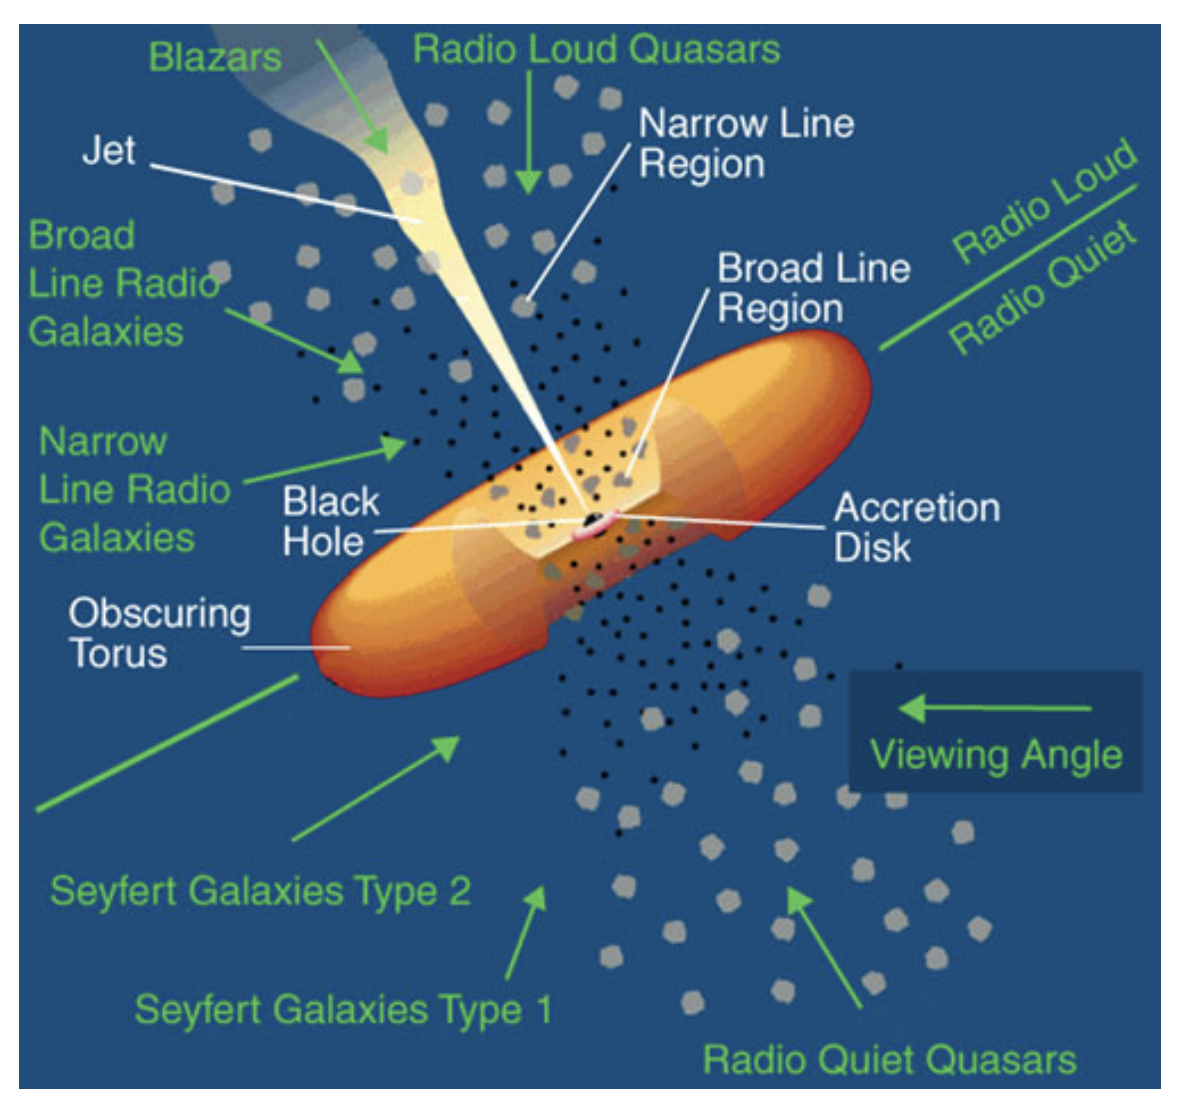
\includegraphics[width=12cm]{figures/extragalactic/AGN.png}}
\end{figure}

{\noindent}The radio jets are launched very close to the central black hole along the direction of the disk axis. The emission from these jets is highly anisotropic, because the velocity in the inner part of the jets is close to the speed of light; then, according to the theory of Special Relativity, the jet emission is strongly beamed in the direction of jet motion. This implies that the appearance of the jet depends on how close the line-of-sight to an observer is to the jet axis. If the jet points almost directly at the observer, the jet emission can outshine all the other radiation from the AGN. 

{\noindent}The QSOs are the most luminous AGNs. Their core luminosity can be as high as a thousand times that of an $L^*$  galaxy. Therefore they can outshine their host galaxy and appear point-like on optical images. For QSOs of lower $L$, their host galaxies were identified and spatially resolved with the HST. According to our current understanding, AGNs are the active cores of galaxies. These galaxies are supposed to be fairly normal galaxies, except for their intense nuclear activity.

{\noindent}The unusually blue color of quasars suggested the possibility of searching for them not only with radio observations but also at optical wavelengths, namely to look for point-like sources with a very blue $U-B$ color index. These photometric surveys were very successful. In fact, many more such sources were found than expected from radio counts. Most of these sources are (nearly) invisible in the radio domain of the spectrum; such sources are called radio-quiet. Their optical properties are virtually indistinguishable from those of quasars. In particular, they have a blue optical energy distribution (of course, since this was the search criterion!), strong and broad emission lines, and in general a high redshift.

{\noindent}Apart from their radio properties, these sources appear to be like quasars. Therefore they were called radio-quiet quasars, or quasi-stellar objects, QSOs. Today this terminology is no longer very common because the clear separation between sources with and without radio emission is not considered valid any more. Radio-quiet quasars also show radio emission if they are observed at sufficiently high sensitivity. In modern terminology, the expression QSO encompasses both the quasars and the radio-quiet QSOs. About 10 times more radio-quiet QSOs than quasars are thought to exist.

{\noindent}In fact, there is as yet not a clear consensus in whether QSOs show a bimodal distribution in their ratio of radio-to-optical luminosity. Figure \ref{fig:qsoradiovsoptical} shows several different samples of AGN; in particular, optically-selected QSOs from the Palomar-Green survey (filled stars) and radio-loud QSOs (open circles). It seems that the ratio between radio and optical luminosity falls into two broad ranges, with a clear gap in between. Therefore, diagrams like that argue in favor of a bimodal distribution. However, this apparent division into two classes can at least partly be attributed to selection effects: the distribution of the radio-to-optical flux ratio depends on the selection of the QSO sample. Obviously, selecting them by their radio emission will favor those with a large $L_\mathrm{radio}/L_\mathrm{opt}$ ratio. Furthermore, the fraction of QSOs for which this ratio is large (i.e., which would be termed as radio-loud QSOs) depends on optical luminosity and on redshift: One finds a significantly higher radio-loud fraction amongst more luminous, and lower-redshift QSOs.

\begin{figure}[h]
    \floatbox[{\capbeside\thisfloatsetup{capbesideposition={right,top},capbesidewidth=4cm}}]{figure}[\FBwidth]
    {\caption{\footnotesize{Radio vs. optical luminosity of AGN, as measured at $5\,{\rm GHz}$ and in the B-band. Different types of AGNs are shown with different symbols: FR I radio galaxies (open triangles), Broad-Line Radio Galaxies (filled circles), radio-loud QSOs (open circles), Seyfert galaxies and LINERs (crosses), and a sample a $(U-B)$ colour-selected bright QSOs, the Palomar-Green sample (filled stars). Source: M. Sikora et al. 2007, Radio Loudness of Active Galactic Nuclei: Observational Facts and Theoretical Implications, ApJ 658, 815, p. 823, Fig. 1. Figure taken from Schneider (2006).}}
    \label{fig:qsoradiovsoptical}}
    {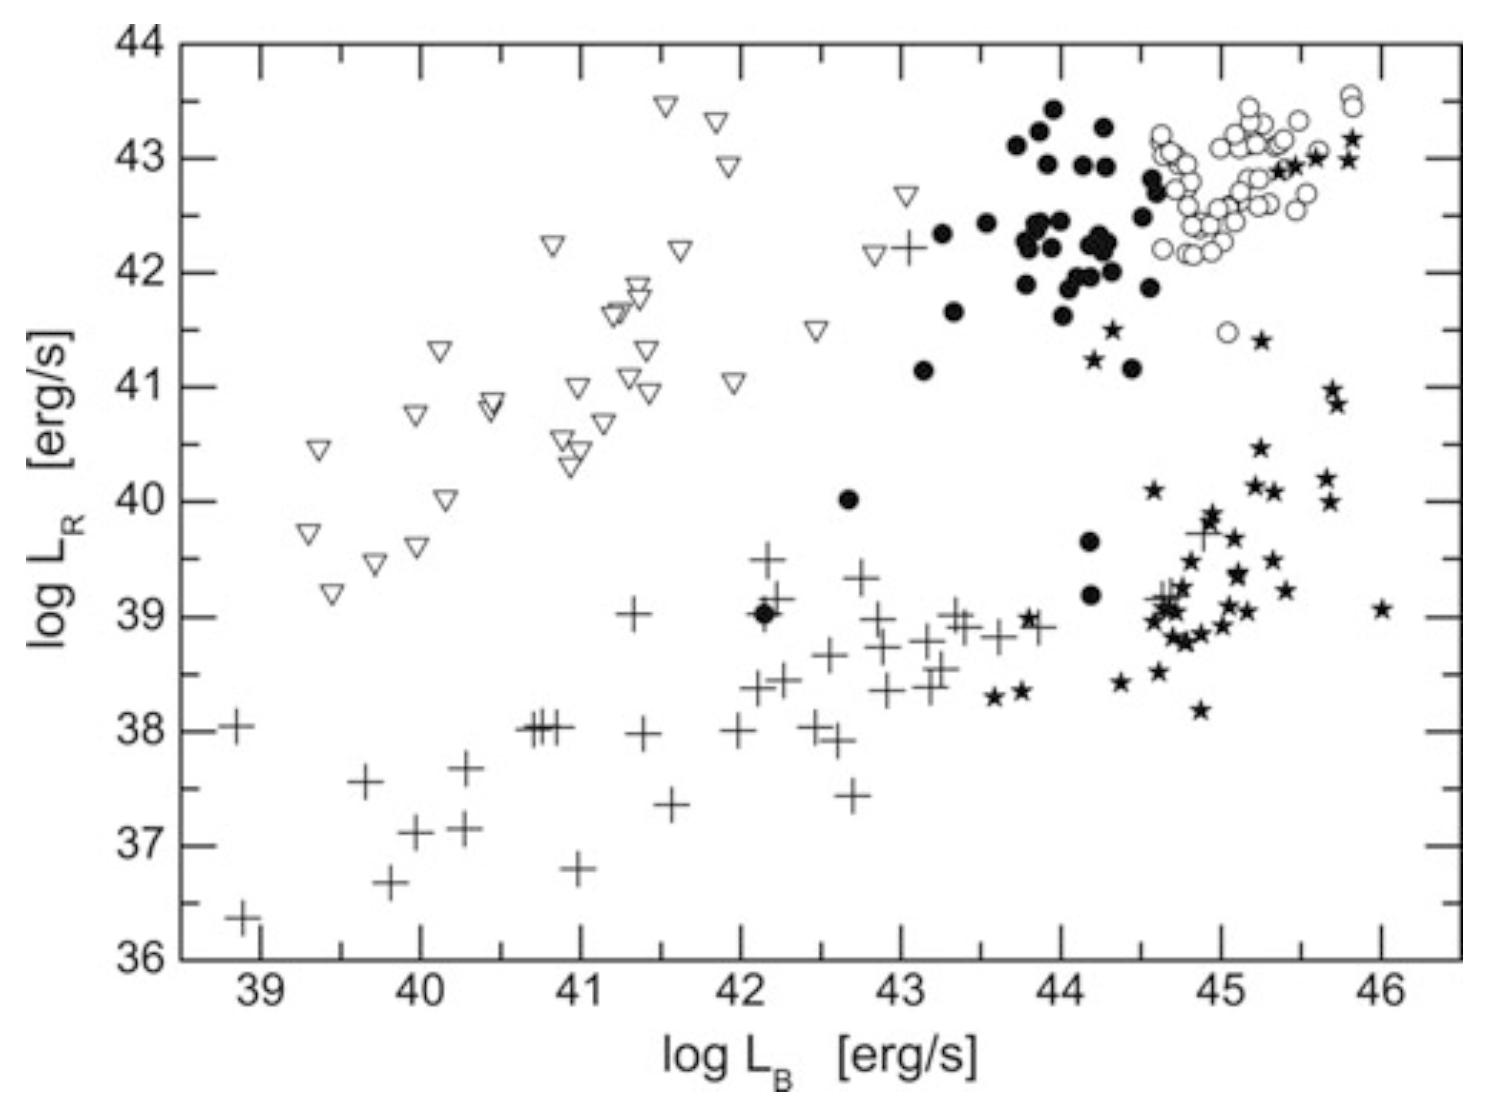
\includegraphics[width=12cm]{figures/extragalactic/QSO_radiovsoptical.png}}
\end{figure}

\begin{figure}[h]
    \floatbox[{\capbeside\thisfloatsetup{capbesideposition={right,top},capbesidewidth=4cm}}]{figure}[\FBwidth]
    {\caption{\footnotesize{Illustration of an accretion disk and a hot corona, where the possible origin of the various X-ray components of an AGN are indicated. Source: L. Gou et al. 2011, The Extreme Spin of the Black Hole in Cygnus X-1, ApJ 742, 85, p. 5, Fig.2. Figure taken from Schneider (2006).}}
    \label{fig:agnaccretion}}
    {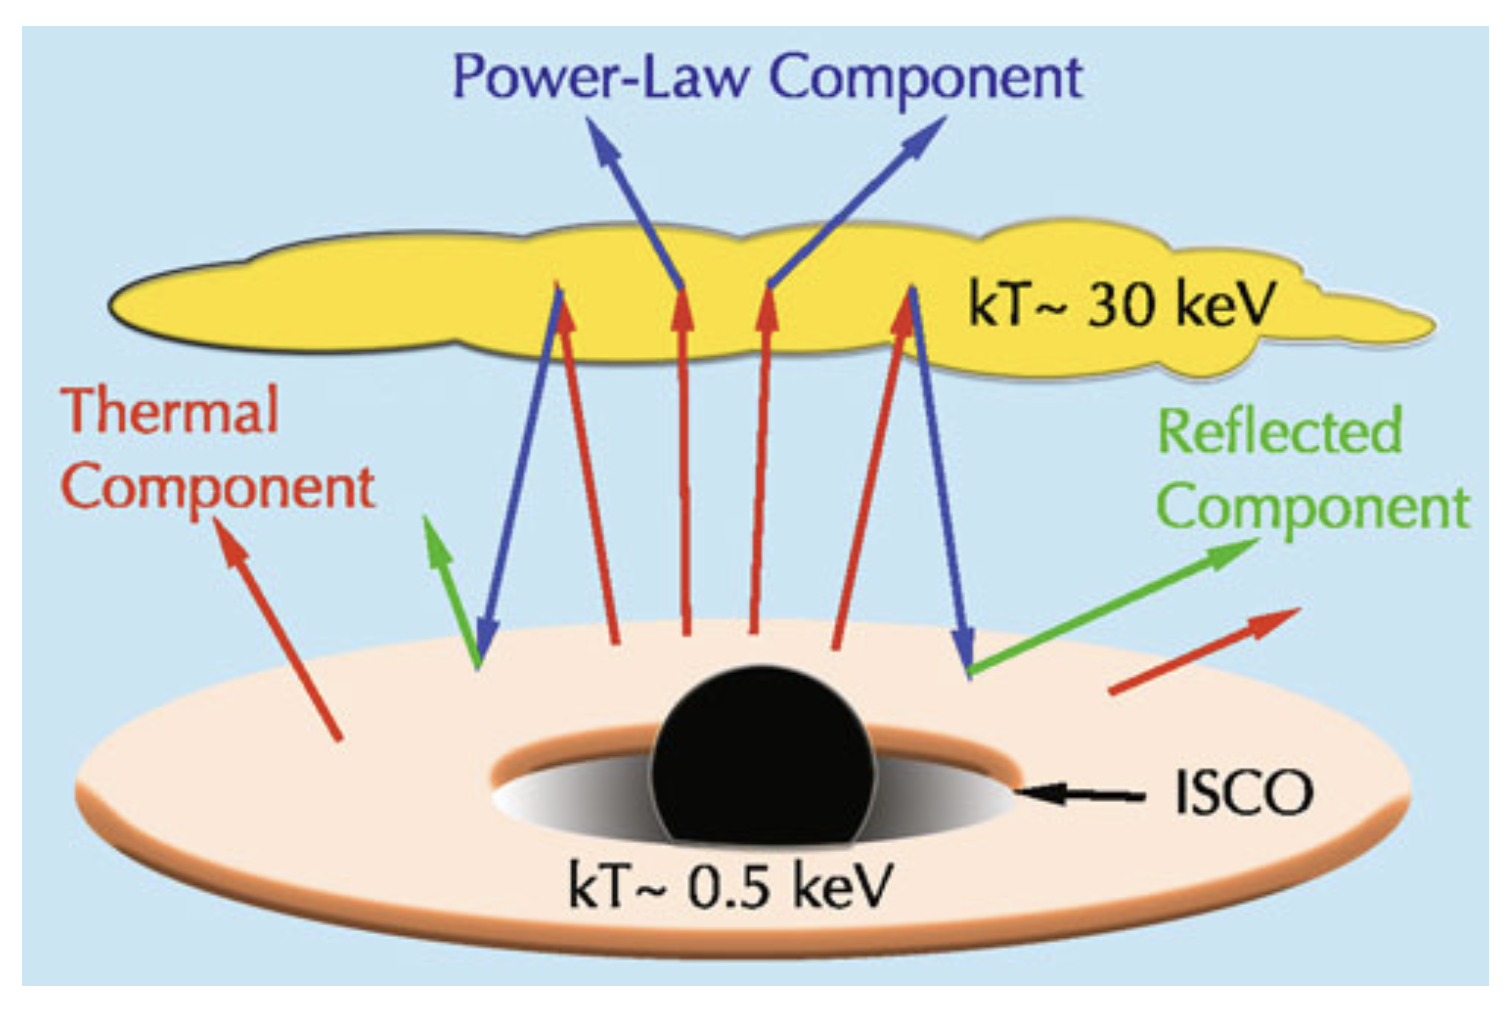
\includegraphics[width=10cm]{figures/extragalactic/AGN_accretion.png}}
\end{figure}

\begin{figure}[h]
    \floatbox[{\capbeside\thisfloatsetup{capbesideposition={right,top},capbesidewidth=4cm}}]{figure}[\FBwidth]
    {\caption{\footnotesize{Illustration of the relativistic jet model. The acceleration of the jet to velocities close to the speed of light is probably caused by a combination of very strong gravitational fields in the vicinity of the SMBH and strong magnetic fields which are rotating rapidly because they are anchored in the accretion disk. Credit: NASA/ESA and Ann Feild, Space Telescope Science Institute Figure taken from Schneider (2006).}}
    \label{fig:agnjet}}
    {\includegraphics[width=10cm]{figures/extragalactic/AGN_jet.png}}
\end{figure}

\subsubsection{Follow-up Questions}

\begin{itemize}
    \item What are the physical scales in this diagram? (Cross section of SMBH, accretion disk and jet.)
    \item How massive are SMBHs?
    \item Why is there a connection between bulge properties and SMBH mass?
    \item How do you determine over what range SMBH potential is important?
\end{itemize}


% --------------------------------------------------------------
%               13. 
% --------------------------------------------------------------

\newpage
\subsection{Question 13}

What are galaxy clusters? What are their basic properties (eg, mass, size). List and explain three ways they can be detected.

\subsubsection{Short answer}

Answer.

\subsubsection{Additional context}

Additional context.

\subsubsection{Follow-up Questions}

\begin{itemize}
    \item (On the X-ray gas method of detection:) Where does it come from?
    \item (On the X-ray gas method of detection:) How do we see it / what is its emission mechanism?
    \item (On the X-ray gas method of detection:) How is the x-ray gas initially heated / why is it hot?
    \item Say more about galaxy interactions in clusters.
    \item Where is most of the mass in a galaxy cluster?
    \item What heats the IGM?
    \item Do optical surveys need redshift information to identify galaxy clusters?
    \item Describe how star formation changes throughout the cluster.
    \end{itemize}



% --------------------------------------------------------------
%               14. 
% --------------------------------------------------------------

\newpage
\subsection{Question 14}

What is star formation quenching? What is the evidence for it, and why is it thought to happen?

\subsubsection{Short answer}

Answer.

\subsubsection{Additional context}

Hydrodynamical simulations of disk formation show that SF in the gas disks is far too efficient, consuming the available gas in too short a time, so that most of the stars would be formed at high redshift, with little current star formation left. Furthermore, the resulting disks are too concentrated and too small, leading to rotation curves which are declining outwards beyond the (small) half-light radius of the disk, in marked contrast with observed rotation curves. This together is known as the overcooling problem in galaxy evolution. Real disk galaxies have a slower conversion of gas into stars and their disks remain larger. And finally, the efficient conversion of gas into stars in our simple model would predict that the stellar mass density in the Universe is much higher than observed -- whereas $\omega_b\sim0.04$, the density parameter in stars is less than 1\%. Hence, most baryons in the Universe have not been converted to stars.

{\noindent}\textbf{Feedback by supernovae:} In order to balance the efficient gas cooling, heating sources need to be considered. An unavoidable source of heating is the energy injected into the ISM by supernovae. Very shortly after star formation sets in, the most massive stars of the stellar population undergo a core-collapse supernova. The mechanical energy of the explosion is partly transferred to the gas surrounding the exploding star. Thereby the gas is heated, causing it to expand, thus to decrease its density, which in turn reduces its cooling efficiency. Note that this is a feedback process -- the higher the star formation rate, the more energy is injected into the interstellar gas to prevent, or at least delay, further SF. Depending on the efficiency of this feedback, the local gas of the disk may be blown out of the disk into the halo (and produce a hot gas corona outside the disk), or, in particular for low-mass halos, be removed from the halo through outflowing gas.

{\noindent}In fact, there is direct observational evidence of the occurrence of outflows from star-forming galaxies. For example, the spectra of Lyman-break galaxies reveal substantial mass outflows, at a similar rate as their star-formation rate and with velocities of several hundreds of ${\rm km\,s^{-1}}$.

{\noindent}The details of this feedback process are somewhat uncertain -- how much of the supernova energy is converted into heat, and how much is transferred to the ISM in form of bulk kinetic energy, is not well determined. Furthermore, the feedback by supernovae depends on the assumed initial mass function of stars, which yields the fraction of newly formed stars which explode as core-collapse supernova. The flatter the IMF at the high-mass end, the more supernova energy per unit mass of newly formed stars is injected.

{\noindent}Assuming a universal IMF, the energy released by supernovae per unit mass of newly-formed stars is $\eta_\mathrm{SN}E_\mathrm{SN}$, where $\eta_\mathrm{SN}$ denotes the expected number of supernovae per unit mass of formed stars, and $E_\mathrm{SN}$ is the energy released per supernova. If we assume that this energy reheats some of the cold gas back to virial temperature of the halo, the amount of gas that is reheated after formation of a group of stars with mass $\Delta m_*$ is

\begin{align*}
    \Delta m_\mathrm{reheat} \sim \epsilon\frac{\eta_\mathrm{SN}E_\mathrm{SN}}{V_{200}^2}\Delta m_* ~ [{\rm M_\odot}],
\end{align*}

{\noindent}where $\epsilon$ parametrizes the efficiency of the reheating process. The reheated gas may be transferred back to the hot gaseous halo, whereas other models assume that the reheated gas is first ejected from the halo, and only later reincorporated into the hot halo on the dynamical time-scale of the halo. This ejection scenario effectively delays the time at which the reheated gas can cool and becomes available for star formation again.

{\noindent}As can be seen from the above equation, supernova feedback is more efficient at suppressing star formation in low-mass galaxies -- which is due to the fact that the binding energy per unit mass is an increasing function of halo mass. This simply expresses the fact that for low-mass halos it is easier to drive the gas outwards.

{\noindent}\textbf{AGN feedback:} Whereas supernova feedback explains a decreasing conversion of gas into stars with decreasing halo mass, and thus can account for the difference of the slopes between the galaxy luminosity function and the halo mass function at the low mass/luminosity end, it is less efficient for higher-mass halos, due to the larger $V_{200}$. The increase of the cooling time for higher-mass halos by itself cannot account for the abrupt exponential decrease of the galaxy luminosity function beyond $L^*$. One requires another process which delays the cooling of gas in high-mass halos.

{\noindent}For very massive halos, we have already encountered such a process: the suppression of cooling flows in galaxy clusters is due to AGN activity of the central galaxy in the cluster. Since (almost) all massive galaxies contain a supermassive black hole, this kind of feedback may be operational not only in groups and clusters, but actually in individual massive galaxies as well. In particular, there is a great deal of evidence for a relation between nuclear starbursts in galaxies and AGN activity. The gas needed for a starburst in the center of a galaxy is also potential fuel for the central black hole. Again, the details of this process are quite uncertain, but with plausible prescriptions, the cut-off of the luminosity function at $L\gtrsim L^*$ can be successfully modeled.

{\noindent}Feedback by an AGN can occur in several ways. In the case of galaxy clusters, the major effect of the AGN is the insertion of hot bubbles into the intracluster medium (ICM) through radio jets. The AGNs in most central cluster galaxies are not very luminous, and seem to be in the `radio mode' of low accretion rate. Thus, for low accretion rates, the main channel of feedback is the injection of mechanical energy into the surrounding gas. At high accretion rates, in the `quasar mode', the main source of feedback is presumably heating of the gas. Furthermore, the strong radiation field from quasars changes the ionization structure of the surrounding gas, which affects its cooling curve compared and at low temperatures actually leads to radiative heating. These various effects should be included in realistic models of the evolution of galaxies, at least in an approximate way.

{\noindent}\textbf{Strangulation:}

\subsubsection{Follow-up Questions}

\begin{itemize}
    \item What is the SF history of the Universe, and how does it evolve with time? (i.e., Lilly-Madau plot.)
    \item At what redshift was the SF rate the highest?
    \item How does this relate to the population of stars we see today (i.e., how old the Sun is, which stars are most common etc.)?
\end{itemize}

% --------------------------------------------------------------
%               15. 
% --------------------------------------------------------------

\newpage
\subsection{Question 15}

Provide three examples of ways in which feedback processes are important on galactic and intergalactic scales.

\subsubsection{Short answer}

Answer.

\subsubsection{Additional context}

Additional context.

\subsubsection{Follow-up Questions}

\begin{itemize}
    \item What is the star formation rate in the galaxy (derive this)? 
    \item How fast would all the gas be eaten up if there was no feedback?
    \item How could you observationally constrain metal enrichment of the IGM?
    \item How do these processes affect a single galaxy (i.e., not a cluster)?
    \item If feedback sets an effective maximum mass for a galaxy, can you draw a cooling curve (i.e., density versus temperature)? 
\end{itemize}

% --------------------------------------------------------------
%               Resources 
% --------------------------------------------------------------

\newpage
\subsection{Resources}

\begin{itemize}
    \item Extragalactic Astronomy and Cosmology, Schneider (2006)
    \item High Energy Astrophysics, Longair (2011)
    \item Gaseous Nebulae and Active Galactic Nuclei, Osterbrock \& Ferland (2005)
    \item Spectral Evolution of Galaxies, Charlot (1996)
    \item Galaxies in the Universe, Sparke \& Gallagher (2005)
    \item Elliptical Galaxies and Bulges of Disk Galaxies: Summary of Progress and Outstanding Issues, Kormendy (2015)
\end{itemize}







































% --------------------------------------------------------------
%
%
%                              GALACTIC 
%
%
% --------------------------------------------------------------

\newpage
\section{Galactic Astronomy}

% --------------------------------------------------------------
%               1. 
% --------------------------------------------------------------

\subsection{Question 1}

What is a stellar Initial Mass Function (IMF)? Sketch it. Give a couple of examples of simple parametric forms used to describe the IMF, such as the Chabrier, Kroupa, or Salpeter functions.

\subsubsection{Short answer}

Answer.

\subsubsection{Additional context}

Since the observable signatures for star formation are obtained only from massive stars, their formation rate needs to be extrapolated to lower masses to obtain the full SFR by assuming an IMF. Typically, a Salpeter-IMF is chosen between $0.1\,M_\odot\geq M\geq 100\,M_\odot$. However, there are clear indications that the IMF may be flatter for $M\gtrsim1\,M_\odot$ than described by the Salpeter law, and several descriptions for such modified IMFs have been developed over the years, mainly based on observations and interpretation of star-forming regions in our MW or in nearby galaxies. The total stellar mass, obtained by integration over the IMF, is up to a factor of $\sim2$ lower in these modified IMFs than for the Salpeter IMF. Thus, this factor provides a characteristic uncertainty in the determination of the SFR from observations; a similar, though somewhat smaller uncertainty applies to the stellar mass density whose estimation also is mainly based on the more massive stars of a galaxy which dominate the luminosity. Furthermore, the IMF need not be universal, but may in principle vary between different environments, or depend on the metallicity of the gas from which stars are formed. Whereas there has not yet been unambiguous evidence for variations of the IMF, this possibility must always be taken into account.

\subsubsection{Follow-up Questions}

\begin{itemize}
    \item How did Salpeter determine the IMF?
    \item How do you normalize the IMF?
    \item Is the upper or lower limit on mass more important for normalization?
\end{itemize}

% --------------------------------------------------------------
%               2. 
% --------------------------------------------------------------

\newpage
\subsection{Question 2}

Describe the orbits of stars in a galactic disk and in galactic spheroid.

\subsubsection{Short answer}

Answer.

\subsubsection{Additional context}

Additional context.

\begin{itemize}
    \item If we perturb a star in the disk in the z-direction, what happens?
    \item If we perturb a star in the disk in the radial-direction, what happens?
    \item What are the observed quantities in each scenario?
    \item How many integrals of motion are there in the disk?
    \item What symmetry leads to energy conservation?
\end{itemize}


% --------------------------------------------------------------
%               3. 
% --------------------------------------------------------------

\newpage
\subsection{Question 3}

Every now and then a supernova explosion occurs within $3\,\mathrm{pc}$ of the Earth. Estimate how long one typically has to wait for this to happen. Why are newborn stars likely to experience this even when they are much younger than the waiting time you have just estimated?

\subsubsection{Short answer}

Answer.

\subsubsection{Additional context}

Additional context.

% --------------------------------------------------------------
%               4. 
% --------------------------------------------------------------

\newpage
\subsection{Question 4}

Galactic stars are described as a collision-less system. Why? (Don’t forget the influence of gravity.)

\subsubsection{Short answer}

Answer.

\subsubsection{Additional context}

Additional context.

\subsubsection{Follow-up Questions}

\begin{itemize}
    \item What happens when stars collide?
    \item Why choose a cross-section that's larger than the star's radius?
    \item What impact parameter do we need for the stars to end up physically touching (calculate it)?
\end{itemize}

% --------------------------------------------------------------
%               5. 
% --------------------------------------------------------------

\newpage
\subsection{Question 5}

Given that only a tiny fraction of the mass of the interstellar medium consists of dust, why is dust important to the chemistry of the medium and to the formation of stars?

\subsubsection{Short answer}

Answer.

\subsubsection{Additional context}

Additional context.

\subsubsection{Follow-up Questions}

\begin{itemize}
    \item Why is molecular hydrogen (H$_2$) so difficult to detect?
    \item What are other ways in which molecular cloud cores cool?
\end{itemize}

% --------------------------------------------------------------
%               6. 
% --------------------------------------------------------------

\newpage
\subsection{Question 6}

The ISM mainly consists of hydrogen and helium, which are very poor coolants. How, then, do molecular cloud cores ever manage to lose enough heat to collapse and form stars? Why are H
and He such poor coolants?

\subsubsection{Short answer}

Answer.

\subsubsection{Additional context}

Additional context.

% --------------------------------------------------------------
%               7. 
% --------------------------------------------------------------

\newpage
\subsection{Question 7}

The stars in the solar neighbourhood, roughly the $300\,\mathrm{pc}$ around us, have a range of ages, metallicities and orbital properties. How are those properties related?

\subsubsection{Short answer}

Answer.

\subsubsection{Additional context}

Additional context.

% --------------------------------------------------------------
%               8. 
% --------------------------------------------------------------

\newpage
\subsection{Question 8}

What are the main sources of heat in the interstellar medium?

\subsubsection{Short answer}

Answer.

\subsubsection{Additional context}

Additional context.

\subsubsection{Follow-up Questions}

\begin{itemize}
    \item Are there any non-ionization sources of heat in the ISM? (shocks)
    \item How do shock waves heat the gas?
    \item Are shock waves adiabatic?
    \item Where do the x-rays for x-ray photoionization come from?
    \item What phases and temperatures of the ISM apply to each example?
\end{itemize}

% --------------------------------------------------------------
%               9. 
% --------------------------------------------------------------

\newpage
\subsection{Question 9}

Draw an interstellar extinction curve (ie, opacity), from the X-ray to the infrared. What are the physical processes responsible?

\subsubsection{Short answer}

Answer.

\subsubsection{Additional context}

Additional context.

\subsubsection{Follow-up Questions}

\begin{itemize}
    \item What happens at shorter wavelengths, like gamma rays?
\end{itemize}

% --------------------------------------------------------------
%               10. 
% --------------------------------------------------------------

\newpage
\subsection{Question 10}

What is dynamical friction? Explain how this operates in the merger of a small galaxy into a large one.

\subsubsection{Short answer}

Answer.

\subsubsection{Additional context}

Additional context.

% --------------------------------------------------------------
%               11. 
% --------------------------------------------------------------

\newpage
\subsection{Question 11}

Sketch the SED, from the radio to Gamma, of a spiral galaxy like the Milky Way. Describe the source and radiative mechanism of each feature.

\subsubsection{Short answer}

Answer.

\subsubsection{Additional context}

Additional context.

\subsubsection{Follow-up Questions}

\begin{itemize}
    \item How do the relative heights of the optical/FIR peaks change?
\end{itemize}

% --------------------------------------------------------------
%               12. 
% --------------------------------------------------------------

\newpage
\subsection{Question 12}

How many stars does one expect to find within $100\,\mathrm{pc}$ of the Sun? If all stars are distributed evenly across the galaxy, how many of these will be B spectral type or earlier? How many are younger than $100\,\mathrm{Myrs}$?

\subsubsection{Short answer}

Answer.

\subsubsection{Additional context}

Additional context.

\subsubsection{Follow-up Questions}

\begin{itemize}
    \item Justify the assumptions made and explain why they do not match observations (e.g., number density of stars in the MW is not a flat distribution, the SFR isn't constant etc.).
    \item Where are most B-type and other early-type stars actually found?
    \item How do we know how many stars are in the MW?
    \item How do we measure the IMF?
    \item Are high- or low-mass stars more important to constrain the total number of stars?
    \item How many B stars are visible from your backyard? Are there any star forming regions visible from your backyard?
\end{itemize}

% --------------------------------------------------------------
%               13. 
% --------------------------------------------------------------

\newpage
\subsection{Question 13}

Describe what happens as a cloud starts to collapse and form a star. What is the difference between the collapse and contraction stages? What happens to the internal temperature in both? When does the contraction phase end, and why does the end point depend on the mass of the object?

\subsubsection{Short answer}

Answer.

\subsubsection{Additional context}

Additional context.

\subsubsection{Follow-up Questions}

\begin{itemize}
    \item \item How do you calculate the Jeans mass?
    \item What happens to the temperature during adiabatic contraction?
    \item Draw a plot of density versus temperature to distinguish between the contracting and collapsing phases.
\end{itemize}

% --------------------------------------------------------------
%               14. 
% --------------------------------------------------------------

\newpage
\subsection{Question 14}

Sketch the rotation curve for a typical spiral galaxy. Show that a flat rotation curve implies the existence of a dark matter halo with a density profile that drops off as $1/r^2$.

\subsubsection{Short answer}

Answer.

\subsubsection{Additional context}

Additional context.

\subsubsection{Follow-up Questions}

\begin{itemize}
    \item What assumptions are made in deriving the $1/r^2$ profile?
\end{itemize}

% --------------------------------------------------------------
%               15. 
% --------------------------------------------------------------

\newpage
\subsection{Question 15}

What thermal phases are postulated to exist in the interstellar medium? Describe the dominant mechanism of cooling for each phase.

\subsubsection{Short answer}

Answer.

\subsubsection{Additional context}

Additional context.

\begin{itemize}
    \item Write down typical temperatures and densities for each phase.
    \item Where do you find each of these phases?
    \item Why don't we see molecular gas (H$_2$) in all of these phases?
    \item Describe what each of these regions might looks like.
    \item How do constituents change between the different thermal phases?
\end{itemize}

% --------------------------------------------------------------
%               16. 
% --------------------------------------------------------------

\newpage
\subsection{Question 16}

Characterize the stellar populations in the following regions: i) the Galactic bulge ii) the Galactic disk, outside of star clusters iii) open star clusters iv) globular clusters v) the Galactic halo vi) a typical elliptical galaxy.

\subsubsection{Short answer}

Answer.

\subsubsection{Additional context}

Additional context.

% --------------------------------------------------------------
%               17. 
% --------------------------------------------------------------

\newpage
\subsection{Question 17}

How can one determine the temperature of a HII region?

\subsubsection{Short answer}

Answer.

\subsubsection{Additional context}

Additional context.

% --------------------------------------------------------------
%               18. 
% --------------------------------------------------------------

\newpage
\subsection{Question 18}

What is the G-dwarf problem in the solar neighborhood?

\subsubsection{Short answer}

Answer.

\subsubsection{Additional context}

Additional context.

\subsubsection{Follow-up Questions}

\begin{itemize}
    \item Is it reasonable to assume that the IMF changes over time? Why?
    \item How much does the mean molecular weight change over cosmological timescales?
    \item What is an appropriate value for the mean molecular weight mu? (i.e., 2 for molecular hydrogen setting limits on formation masses.)
    \item Do we talk about upper mass limits because more massive stars can't exist, or because they don't exist?
\end{itemize}



% --------------------------------------------------------------
%               19. 
% --------------------------------------------------------------

\newpage
\subsection{Question 19}

Describe the general characteristics of spiral structure in galaxies.

\subsubsection{Short answer}

Answer.

\subsubsection{Additional context}

Additional context.

% --------------------------------------------------------------
%               Resources 
% --------------------------------------------------------------

\newpage
\subsection{Resources}

\begin{itemize}
    \item Galaxy Formation, Longair (2008)
    \item Galaxies in the Universe, Sparke \& Gallagher (2007)
    \item Galactic Dynamics, Binney \& Tremaine (2011)
    \item Galaxies: Interactions and Induced Star Formation, Kennicutt, Schweizer \& Barnes (1996)
    \item Stellar Populations, Greggio \& Renzini (2011)
    \item Physics of the Interstellar and Intergalactic Medium, Draine (2011)
    \item Astrophysics of the Interstellar Medium, Maciel (2013)
    \item Notes on Star Formation, Krumholz (2015)
    \item Principles of Star Formation, Bodenheimer (2011)
\end{itemize}






































% --------------------------------------------------------------
%
%
%                              STARS 
%
%
% --------------------------------------------------------------

\newpage
\section{Stellar Astrophysics}

% --------------------------------------------------------------
%               1. 
% --------------------------------------------------------------

\subsection{Question 1}

Sketch out a Hertsprung-Russell diagram. Indicate where on the main sequence different spectral classes lie. Draw and describe the post main-sequence tracks of both low- and high-mass stars.

\subsubsection{Short answer}

Answer.

\subsubsection{Additional context}

Additional context.

\begin{itemize}
    \item How does metallicity affect this diagram?
    \item Elaborate on the life sequence of low-mass stars.
    \item Elaborate on the life sequence of high-mass stars.
    \item Which direction does radius increase?
    \item What's the functional form for how radius increases as a function of temperature and luminosity?
    \item Why can you use the tip of the red giant branch for distance determination?
    \item How can you use the H-R diagram to determine ages? Which of the two techniques is more accurate?
\end{itemize}

% --------------------------------------------------------------
%               2. 
% --------------------------------------------------------------

\newpage
\subsection{Question 2}

Sketch a plot of radius versus mass for various ``cold'' objects made of normal matter, including planets, brown dwarfs and white dwarfs. Explain the mass-size relationship for rocky and
gaseous objects. Why is there an upper mass limit?

\subsubsection{Short answer}

Answer.

\subsubsection{Additional context}

Additional context.

\subsubsection{Follow-up Questions}

\begin{itemize}
    \item How do you calculate the Chandrasekhar mass limit?
    \item Why is Saturn smaller than Jupiter? Or, why do we see a range of radii in extrasolar planets (e.g., hot Jupiters)?
\end{itemize}

% --------------------------------------------------------------
%               3. 
% --------------------------------------------------------------

\newpage
\subsection{Question 3}

Describe the physical conditions that lead to the formation of absorption lines in stars' spectra. What leads to emission lines?

\subsubsection{Short answer}

Answer.

\subsubsection{Additional context}

Additional context.

\subsubsection{Follow-up Questions}

\begin{itemize}
    \item Why aren't emission and absorption lines delta functions?
    \item How does this relate to population levels and excitation temperatures?
    \item Are there emission lines in the Sun? Why is there emission from the Calcium doublet?
    \item Write down the heat transfer equation. What do solutions look like?
\end{itemize}

% --------------------------------------------------------------
%               4. 
% --------------------------------------------------------------

\newpage
\subsection{Question 4}

Describe these important sources of stellar opacity: electron scattering, free-free, bound-free, and the H$^-$ ion.

\subsubsection{Short answer}

Answer.

\subsubsection{Additional context}

Additional context.

% --------------------------------------------------------------
%               5. 
% --------------------------------------------------------------

\newpage
\subsection{Question 5}

Describe the processes that can cause pulsations in a star’s luminosity, and provide at least one example of a class of stellar pulsation.

\subsubsection{Short answer}

Answer.

\subsubsection{Additional context}

Additional context.

\subsubsection{Follow-up Questions}

\begin{itemize}
    \item What about the instability strip? RR Lyrae?
    \item What is the period-luminosity relation?
    \item What is the form of the period-luminosity relation?
    \item How would you derive the time scale of pressure waves in a star?
    \item How would you order-of-magnitude estimate the period for a pulsation?
\end{itemize}

% --------------------------------------------------------------
%               6. 
% --------------------------------------------------------------

\newpage
\subsection{Question 6}

Briefly describe the sources of thermal energy for stars and planets.

\subsubsection{Short answer}

Answer.

\subsubsection{Additional context}

Additional context.

\subsubsection{Follow-up Questions}

\begin{itemize}
    \item Why do different nuclear reaction pathways have different temperature sensitivities?
    \item If I assume a constant core temperature on the main sequence, how does stellar radius depend on mass?
    \item What are some other thermal sources, like say for neutron stars?
\end{itemize}

% --------------------------------------------------------------
%               7. 
% --------------------------------------------------------------

\newpage
\subsection{Question 7}

Describe the process by which supernovae produce light. Why are Type Ia supernovae generally brighter than Type II events?

\subsubsection{Short answer}

Answer.

\subsubsection{Additional context}

Additional context.

\subsubsection{Follow-up Questions}

\begin{itemize}
    \item When a star goes supernova, how much of the luminous energy generated at the rebound is available for heating the gas? As in, where does the heat come from?
    \item Are there cases where the rebound shock wave can't blow up the star? Why, and what happens then?
\end{itemize}

% --------------------------------------------------------------
%               8. 
% --------------------------------------------------------------

\newpage
\subsection{Question 8}

Describe the condition for a star’s envelope to become convective. Why are low mass stars convective in their outer envelopes while high mass stars are convective in their inner cores?

\subsubsection{Short answer}

Answer.

\subsubsection{Additional context}

Additional context.

\subsubsection{Follow-up Questions}

\begin{itemize}
    \item How do we know that the Sun's outer envelope is convective?
    \item How far into the surface of the Sun does the convective zone permeate? How can we measure this?
\end{itemize}

% --------------------------------------------------------------
%               9. 
% --------------------------------------------------------------

\newpage
\subsection{Question 9}

What is Eddington’s luminosity limit? Explain why this limit is important for the properties and lifetimes of massive stars.

\subsubsection{Short answer}

Answer.

\subsubsection{Additional context}

Additional context.

\subsubsection{Follow-up Questions}

\begin{itemize}
    \item Draw a force diagram of what’s happening.
    \item What particles experience gravity the most?
    \item What particles experience photon pressure the most?
\end{itemize}

% --------------------------------------------------------------
%               10. 
% --------------------------------------------------------------

\newpage
\subsection{Question 10}

Explain why we know what the Sun’s central temperature ought to be, and how we know what it actually is.

\subsubsection{Short answer}

Answer.

\subsubsection{Additional context}

Additional context.

% --------------------------------------------------------------
%               11. 
% --------------------------------------------------------------

\newpage
\subsection{Question 11}

Which have higher central pressure, high-mass or low-mass main-sequence stars? Roughly, what is their mass-radius relation? Derive this.

\subsubsection{Short answer}

Answer.

\subsubsection{Additional context}

Additional context.
\subsubsection{Follow-up Questions}

\begin{itemize}
    \item How would we actually know the central pressure?
    \item What properties can we measure to test models of stellar structure?
\end{itemize}

% --------------------------------------------------------------
%               12. 
% --------------------------------------------------------------

\newpage
\subsection{Question 12}

Sketch the SED of an O, A, G, M, and T star. Give defining spectral characteristics, such as the Balmer lines and Balmer jump and Calcium doublets, and describe physically.

\subsubsection{Short answer}

Answer.

\subsubsection{Additional context}

Additional context.

\subsubsection{Follow-up Questions}

\begin{itemize}
    \item Are there emission lines?
    \item What molecular lines are in the Sun?
    \item What important lines are there are much longer wavelengths than those in the optical?
    \item What if the A star had a protoplanetary disk?
    \item What is the significance of a $\lambda$F$_\lambda$ (or $\nu$F$_\nu$) spectrum?
    \item How can the relative height of the stellar vs disk bumps change? (i.e., total energy of the system cannot change; dust bump can't be higher than star bump without extinction.)
\end{itemize}

% --------------------------------------------------------------
%               13. 
% --------------------------------------------------------------

\newpage
\subsection{Question 13}

What can be learned about young stars (T Tauri and pre-main-sequence stars) from an analysis of their spectral features?

\subsubsection{Short answer}

Answer.

\subsubsection{Additional context}

Additional context.

\subsubsection{Follow-up Questions}

\begin{itemize}
    \item How does the spectrum change as planets start to form?
\end{itemize}

% --------------------------------------------------------------
%               14. 
% --------------------------------------------------------------

\newpage
\subsection{Question 14}

Sketch the spectral energy distribution (SED) of a T Tauri star surrounded by a protoplanetary disk. How would the SED change: (a) if the disk develops a large inner hole, (b) if the dust grains in the disk grow in size by agglomeration (with the same total mass)?

\subsubsection{Short answer}

Answer.

\subsubsection{Additional context}

Additional context.

% --------------------------------------------------------------
%               15. 
% --------------------------------------------------------------

\newpage
\subsection{Question 15}

What are the primary origins of the heat lost to space by infrared luminosity of Jupiter, Earth, and Io?

\subsubsection{Short answer}

Answer.

\subsubsection{Additional context}

Additional context.

% --------------------------------------------------------------
%               16. 
% --------------------------------------------------------------

\newpage
\subsection{Question 16}

Explain the observational problem of radius inflation for hot Jupiters and describe two possible solutions.

\subsubsection{Short answer}

Answer.

\subsubsection{Additional context}

Additional context.

% --------------------------------------------------------------
%               17. 
% --------------------------------------------------------------

\newpage
\subsection{Question 17}

Explain the effects of an atmosphere on a planet’s surface temperature and the position of the “habitable zone”. What special considerations must one make for habitability around M-type stars?

\subsubsection{Short answer}

Answer.

\subsubsection{Additional context}

Additional context.

% --------------------------------------------------------------
%               18. 
% --------------------------------------------------------------

\newpage
\subsection{Question 18}

Explain the process of nuclear fusion and give two examples of important fusion processes that affect the lives of stars.

\subsubsection{Short answer}

Answer.

\subsubsection{Additional context}

Additional context.

% --------------------------------------------------------------
%               19. 
% --------------------------------------------------------------

\newpage
\subsection{Question 19}

What is Fermi’s Paradox? Explain its logic and assess the current state of the Paradox in light of modern knowledge.

\subsubsection{Short answer}

Answer.

\subsubsection{Additional context}

Additional context.

\subsubsection{Follow-up Questions}

\begin{itemize}
    \item What percentage of stars have planets?
\end{itemize}

% --------------------------------------------------------------
%               20. 
% --------------------------------------------------------------

\newpage
\subsection{Question 20}

The so-called r- and s- processes are mechanisms that produce elements heavier than iron. Describe these mechanisms and evidence for them from abundance patterns. Where is the r-process thought to act?

\subsubsection{Short answer}

Answer.

\subsubsection{Additional context}

Additional context.

% --------------------------------------------------------------
%               Resources 
% --------------------------------------------------------------

\newpage
\subsection{Resources}

\begin{itemize}
    \item The Fundamentals of Stellar Astrophysics, Collins (2003)
    \item Stellar Structure and Evolution, Kippenhahn, Weigert \& Weiss (2012)
    \item Evolution of Stars and Stellar Populations, Salaris \& Cassisi (2005)
    \item The Astronomical Reach of Fundamental Physics, Burrows \& Ostriker (2014)
    \item Opacity, Huebner \& Barfield (2014)
    \item Radiative Processes in Astrophysics, Rybicky \& Lightman (1979)
    \item Understanding Variable Stars, Percy (2007)
\end{itemize}









































% --------------------------------------------------------------
%
%
%                              PHYSICS 
%
%
% --------------------------------------------------------------

\newpage
\section{Physics}

% --------------------------------------------------------------
%               1. 
% --------------------------------------------------------------

\subsection{Question 1}

Draw the geometry of gravitational microlensing of one star by another, and estimate the angular displacement of the background star's image.

\subsubsection{Short answer}

Answer.

\subsubsection{Additional context}

Additional context.

\subsubsection{Follow-up Questions}

\begin{itemize}
    \item Can you derive $\phi$ from a Newtonian approach?
    \item Why/how does gravitational lensing magnify a star?
\end{itemize}

% --------------------------------------------------------------
%               2. 
% --------------------------------------------------------------

\newpage
\subsection{Question 2}

A two-element interferometer consists of two telescopes whose light is combined and interfered. Sketch the response of such an interferometer to a nearby red giant star, as a function
of the (projected) separation between the two telescopes. The red giant subtends one-fiftieth of an arc second on the sky, and the telescope operates at a wavelength of 2 microns.

\subsubsection{Short answer}

Answer.

\subsubsection{Additional context}

Additional context.

\subsubsection{Follow-up Questions}

\begin{itemize}
    \item What do the minima in the response function tell you?
\end{itemize}

% --------------------------------------------------------------
%               3. 
% --------------------------------------------------------------

\newpage
\subsection{Question 3}

What's the minimum mass of a black hole you could survive a fall through the event horizon without being ripped to shreds? Why would you be ripped to shreds for smaller black holes? How does this relate to the BH mass range for which we expect tidal disruption flares caused by shredding main-sequence stars?

\subsubsection{Short answer}

Answer.

\subsubsection{Additional context}

Additional context.

\subsubsection{Follow-up Questions}

\begin{itemize}
    \item How would you estimate the maximum tidal acceleration a star can withstand?
    \item Why is it enough to know if the surface of the star will be disrupted?
\end{itemize}

% --------------------------------------------------------------
%               4. 
% --------------------------------------------------------------

\newpage
\subsection{Question 4}

How is synchrotron radiation generated, and how was it used to demonstrate the energy required to power radio galaxies?

\subsubsection{Short answer}

Answer.

\subsubsection{Additional context}

Additional context.

% --------------------------------------------------------------
%               5. 
% --------------------------------------------------------------

\newpage
\subsection{Question 5}

What are ``forbidden lines'' of atomic spectra? In what conditions are they observationally important? In what conditions do they control the temperature of interstellar material?

\subsubsection{Short answer}

Answer.

\subsubsection{Additional context}

Additional context.

\subsubsection{Follow-up Questions}

\begin{itemize}
    \item What are some common examples of forbidden lines?
    \item When do you get forbidden line absorption?
    \item What kind of radiation can be absorbed by forbidden line absorption?
    \item Can we observe any forbidden lines on Earth?
    \item What is the lifetime of the 21 cm line?
    \item At what redshifts do CMB photons get absorbed by 21 cm transitions?
    \item At what redshifts do you get neutral hydrogen?
    \item How would you estimate the lifetime from the maximum density where the line isn't washed out?
    \item Collisions happen much more frequently; why is the 21 cm line still visible?
    \item Why does forbidden line emission cool the gas?
    \item Why are they \textit{so good} at cooling the gas?
\end{itemize}

% --------------------------------------------------------------
%               6. 
% --------------------------------------------------------------

\newpage
\subsection{Question 6}

What is a polytropic equation of state? Give examples of objects for which this is a very good approximation, and explain why it is.

\subsubsection{Short answer}

Answer.

\subsubsection{Additional context}

Additional context.

% --------------------------------------------------------------
%               7. 
% --------------------------------------------------------------

\newpage
\subsection{Question 7}

What was the solar neutrino problem, and how was it resolved?

\subsubsection{Short answer}

Answer.

\subsubsection{Additional context}

Additional context.

\subsubsection{Follow-up Questions}

\begin{itemize}
    \item Can neutrinos account for all of the dark matter in the Universe?
    \item If there was a fourth neutrino flavour, how would we detect it?
    \item Why is the first step of the p-p chain not where we looked for neutrino signatures? (i.e., not energetic enough)
\end{itemize}

% --------------------------------------------------------------
%               8. 
% --------------------------------------------------------------

\newpage
\subsection{Question 8}

Why is nuclear fusion stable inside a main-sequence star? Under what conditions is nuclear fusion unstable? Give examples of actual objects.

\subsubsection{Short answer}

Answer.

\subsubsection{Additional context}

Additional context.

\subsubsection{Follow-up Questions}

\begin{itemize}
    \item Can main sequence stars have unstable nuclear fusion?
    \item If I suddenly increase the core temperature of a star by 20\%, how quickly does the star respond?
    \item What happens when you ignite fusion in a white dwarf? Explain using explicit thermodynamics what happens when you turn up the temperature or reaction rate in the core of the star (i.e. explain adiabatic expansion and contraction).
\end{itemize}

% --------------------------------------------------------------
%               9. 
% --------------------------------------------------------------

\newpage
\subsection{Question 9}

Why do neutrons inside a neutron star not decay into protons and electrons?

\subsubsection{Short answer}

Answer.

\subsubsection{Additional context}

Additional context.

\subsubsection{Follow-up Questions}

\begin{itemize}
    \item What sort of products come from NS-NS mergers?
    \item What are typical photon energies emitted from each of these scenarios?
\end{itemize}

% --------------------------------------------------------------
%               10. 
% --------------------------------------------------------------

\newpage
\subsection{Question 10}

What is the typical temperature of matter accreting on a star, a white dwarf, a neutron star, a stellar mass black hole, and a supermassive black hole? In what wavelength range would one best find examples of such sources?

\subsubsection{Short answer}

Answer.

\subsubsection{Additional context}

Additional context.

\subsubsection{Follow-up Questions}

\begin{itemize}
    \item How does the accretion process work?
    \item If you don't assume a blackbody, and just dump a bunch of material onto a star and it can't radiate away, what is the maximum temperature it can reach?
\end{itemize}

% --------------------------------------------------------------
%               11. 
% --------------------------------------------------------------

\newpage
\subsection{Question 11}

You don't usually need to cool down the detectors for short wavelength (e.g., X-ray) observations, but it's critical to cool down the detectors in long wavelength (e.g., far-IR) observations. Why is this, and why is it not necessary for radio observations?

\subsubsection{Short answer}

Answer.

\subsubsection{Additional context}

Additional context.
% --------------------------------------------------------------
%               12. 
% --------------------------------------------------------------

\newpage
\subsection{Question 12}

Compare the S/N ratios between the following two cases where photon noise is dominant (assume an unresolved point source): [A] 1-minute exposure with a 10-m telescope; [B] 10-minute exposure with a 1-m telescope.

\subsubsection{Short answer}

Answer.

\subsubsection{Additional context}

Additional context.

% --------------------------------------------------------------
%               13. 
% --------------------------------------------------------------

\newpage
\subsection{Question 13}

Describe linear and circular polarizations of electromagnetic waves and give examples of their relevance to astronomical observations.

\subsubsection{Short answer}

Answer.

\subsubsection{Additional context}

Additional context.

% --------------------------------------------------------------
%               14. 
% --------------------------------------------------------------

\newpage
\subsection{Question 14}

What's the field of view of a $2{\rm K}\,\times\,2{\rm K}$ CCD camera on a $5\,{\rm m}$ telescope with $f/16$ focal ratio? The pixel size of the CCD is $20\,\mu$m. Now, let’s bring this to a $10\,{\rm m}$ telescope with the same focal ratio. Explain how the field of view changes on the $10\,{\rm m}$ telescope (compared to that of the $5\,{\rm m}$ telescope) based on the Etendue conservation rule.

\subsubsection{Short answer}

Answer.

\subsubsection{Additional context}

Additional context.

\subsubsection{Follow-up Questions}

\begin{itemize}
    \item If you wanted a smaller FOV with the same size telescope, what would you change?
\end{itemize}

% --------------------------------------------------------------
%               15. 
% --------------------------------------------------------------

\newpage
\subsection{Question 15}

Sketch and give the equations for each of the following distributions: 1. Gaussian (Normal distribution); 2. Poisson distribution; 3. Log-normal distribution. Give two examples from astrophysics where each of these distributions apply.

\subsubsection{Short answer}

Answer.

\subsubsection{Additional context}

Additional context.

\subsubsection{Follow-up Questions}

\begin{itemize}
    \item What sort of noise do you expect for these?
    \item What extra sources of noise can you get from a CCD?
    \item Where does the noise come from, and what does the variance/standard deviation actually tell you?
    \item What property of the Gaussian distribution makes it particularly useful? (i.e., Central limit theorem.)
    \item How do we get a log-normal distribution?
    \item Why do we quote n-sigma probabilities and confidence levels with a Gaussian assumption when the actual probability distribution might not be Gaussian?
    \item If I'm doing a cosmological survey and I say I assume a Poisson distribution for radio galaxy sources and a Gaussian distribution for dust sources, why would I use two different distributions?
\end{itemize}

% --------------------------------------------------------------
%               16. 
% --------------------------------------------------------------

\newpage
\subsection{Question 16}

You are trying to determine a flux from a CCD image using aperture photometry, measuring source(+sky) within a 5-pixel radius, and sky within a 20-25 pixel annulus. Assume you find 10000 electrons inside the aperture and 8100 electrons in the sky region, and that the flux calibration is good to 1\%. What is the fractional precision of your measurement? (Ignore read noise.) More generally, describe how you propagate uncertainties, what assumptions you implicitly make, and how you might estimate errors if these assumptions do not hold.

\subsubsection{Short answer}

Answer.

\subsubsection{Additional context}

Additional context.

% --------------------------------------------------------------
%               17. 
% --------------------------------------------------------------

\newpage
\subsection{Question 17}

Suppose you measure the brightness of a star ten times (in a regime where source- noise dominates. (1) How do you calculate the mean, median, and mode and standard deviation? (2) How can you tell if any points are outliers? Say some points are outliers, what do you do now (i.e., how does this impact the calculation of the quantities in part 1)?

\subsubsection{Short answer}

Answer.

\subsubsection{Additional context}

Additional context.

\subsubsection{Follow-up Questions}

\begin{itemize}
    \item How would you go about fitting a model to your data? (i.e., Bayesian approach.)
    \item Why is using a gaussian generally a good choice?
\end{itemize}

% --------------------------------------------------------------
%               18. 
% --------------------------------------------------------------

\newpage
\subsection{Question 18}

Suppose you do an imaging search for binaries for a sample of 50 stars, and that you find companions in 20 cases. What binary fraction do you infer? Suppose a binary- star fraction of 50\% had been found previously for another sample (which was much larger, so you can ignore its uncertainty). Determine the likelihood that your result is consistent with that fraction.

\subsubsection{Short answer}

Answer.

\subsubsection{Additional context}

Additional context.

% --------------------------------------------------------------
%               19. 
% --------------------------------------------------------------

\newpage
\subsection{Question 19}

What are the primary wavelength bands at which searches for gravitational waves are conducted? What techniques are used to search in each band? What are the sources of gravitational waves in each band? What can we learn from detections (or non-detections)?

\subsubsection{Short answer}

Answer.

\subsubsection{Additional context}

Additional context.

% --------------------------------------------------------------
%               20. 
% --------------------------------------------------------------

\newpage
\subsection{Question 20}

Self-similarity is a useful idealization of many astrophysical systems. Explain what self- similarity means, when it works, and why it is so useful, and provide two examples from any field.

\subsubsection{Short answer}

Answer.

\subsubsection{Additional context}

Additional context.

% --------------------------------------------------------------
%               21. 
% --------------------------------------------------------------

\newpage
\subsection{Question 21}

Explain why diffraction-limited detectors tend to have sidelobes, and how sidelobes can be suppressed in optical and radio observations.

\subsubsection{Short answer}

Answer.

\subsubsection{Additional context}

Additional context.

% --------------------------------------------------------------
%               Resources 
% --------------------------------------------------------------

\newpage
\subsection{Resources}

\begin{itemize}
    \item Astronomical Statistics, Taylor (2004)
    \item Statistical Methods for Astronomical Data Analysis, Chattopadhyay \& Chattopadhyay (2014)
    \item Data Reduction and Error Analysis for the Physical Sciences, Bevington \& Robinson (2003)
    \item Bayesian Logical Data Analysis for the Physical Sciences, Gregory (2005)
    \item Magnetic Fields in Diffuse Media, Lazarian (2015)
    \item Optics, Hecht (2002)
    \item Astronomical Optics, Schroeder (1987)
    \item Handbook of CCD Astronomy, Howell (2006)
    \item Gravitational Waves, Thorne (1994)
    \item Gravitational Bending of Light, Edwards (2007)
    \item Gravitational Lensing, Abdo
    \item Principles of Interferometry, Jackson (2008)
\end{itemize}






































%%%%%%%%%%%%%%%%%%%%%%%%%%%%%%%%%%%%%%%%%%%%%%%%%%%%%%%%
%                                                      %
%                                                      %
%                      APPENDIX                        %
%                                                      %
%                                                      %
%%%%%%%%%%%%%%%%%%%%%%%%%%%%%%%%%%%%%%%%%%%%%%%%%%%%%%%%

\newpage
\section{Appendix}

%%%%%%%%%%%%%%%%%%%%%%%%%%%%%%%%%%%%%%%%%%%%%%%%%%%%%%%%
%                                                      %
%                                                      %
%                      ACRONYMS                        %
%                                                      %
%                                                      %
%%%%%%%%%%%%%%%%%%%%%%%%%%%%%%%%%%%%%%%%%%%%%%%%%%%%%%%%

\subsection{Acronyms}

{\noindent}\textbf{AGN}: active galactic nuclei

{\noindent}\textbf{AU}: astronomical unit

{\noindent}\textbf{BAOs:} baryonic acoustic oscillations

{\noindent}\textbf{BB:} Big Bang or blackbody

{\noindent}\textbf{BBN:} Big Bang nucleosynthesis

{\noindent}\textbf{bf:} bound-free

{\noindent}\textbf{BH:} black hole

{\noindent}\textbf{CCD:} charged couple device

{\noindent}\textbf{CCD:} colour-colour diagram

{\noindent}\textbf{CIB:} Cosmic Infrared Background

{\noindent}\textbf{CMB:} Cosmic Microwave Background

{\noindent}\textbf{CMD:} colour-magnitude diagram

{\noindent}\textbf{CNB:} Cosmic Neutrino Background

{\noindent}\textbf{COBE:} COsmic Background Explorer

{\noindent}\textbf{CDM:} cold dark matter

{\noindent}\textbf{CIB:} cosmic infrared background

{\noindent}\textbf{CMB:} cosmic microwave background

{\noindent}\textbf{CR:} cosmic ray

{\noindent}\textbf{CRB:} cosmic radio background

{\noindent}\textbf{CGB:} cosmic gamma-ray background

{\noindent}\textbf{CUVOB:} cosmic ultraviolet/optical background

{\noindent}\textbf{CXB:} cosmic x-ray background

{\noindent}\textbf{DE:} dark energy

{\noindent}\textbf{DM:} dark matter

{\noindent}\textbf{DM:} distance modulus

{\noindent}\textbf{EoR:} epoch of reionization

{\noindent}\textbf{ff:} free-free

{\noindent}\textbf{FIR:} far infrared

{\noindent}\textbf{GUT:} grand unified theory

{\noindent}\textbf{HRD}: Hertzsprung-Russel diagram

{\noindent}\textbf{ICM:} intracluster medium

{\noindent}\textbf{IGM:} intergalactic medium

{\noindent}\textbf{IMF:} initial mass function

{\noindent}\textbf{IR:} infrared

{\noindent}\textbf{ISM:} interstellar medium

{\noindent}\textbf{RJ:} Rayleigh-Jeans

{\noindent}\textbf{LMC:} Large Magellanic Cloud

{\noindent}\textbf{LTE:} local thermodynamic equilibrium

{\noindent}\textbf{MW:} Milky Way

{\noindent}\textbf{MWG:} Milky Way Galaxy

{\noindent}\textbf{NLTE:} non-local thermodynamic equilibrium

{\noindent}\textbf{NS:} neutron star

{\noindent}\textbf{pc}: parsec

{\noindent}\textbf{PL}: period-luminosity

{\noindent}\textbf{PSF} point-spread function

{\noindent}\textbf{QFT:} quantum field theory

{\noindent}\textbf{QSO:} quasi-stellar object

{\noindent}\textbf{RT:} radiative transfer

{\noindent}\textbf{RTE:} radiative transfer equation

{\noindent}\textbf{SED:} spectral energy distribution

{\noindent}\textbf{SF:} star formation

{\noindent}\textbf{SFR:} star formation rate

{\noindent}\textbf{SMBH:} supermassive black hole

{\noindent}\textbf{S/N:} signal-to-noise

{\noindent}\textbf{SNR:} signal-to-noise ratio

{\noindent}\textbf{TE:} thermal equilibrium

{\noindent}\textbf{TE:} thermodynamic equilibrium

{\noindent}\textbf{WD:} white dwarf

{\noindent}\textbf{$\Lambda$CDM:} $\Lambda$ cold dark matter

{\noindent}\textbf{2dFGRS:} 2 degree Field Galactic Redshift Survey







































%%%%%%%%%%%%%%%%%%%%%%%%%%%%%%%%%%%%%%%%%%%%%%%%%%%%%%%%
%                                                      %
%                                                      %
%                     VARIABLES                        %
%                                                      %
%                                                      %
%%%%%%%%%%%%%%%%%%%%%%%%%%%%%%%%%%%%%%%%%%%%%%%%%%%%%%%%

\newpage
\subsection{Variables}

{\noindent}\textbf{Absorption coefficient}: $\alpha_\nu ~ [{\rm cm^{-1}}]$

{\noindent}\textbf{Angstr\"{o}m}: \AA$ ~ [{\rm unit}]$

{\noindent}\textbf{Angular diameter distance}: $d_A ~ [{\rm pc}]$

{\noindent}\textbf{Angular size}: $\theta ~ [{\rm rad}]$

{\noindent}\textbf{Binding energy of deuterium}: $E_\mathrm{D} ~ [{\rm MeV}]$

{\noindent}\textbf{Binding energy of helium}: $E_\mathrm{He} ~ [{\rm MeV}]$

{\noindent}\textbf{Binding energy of hydrogen}: $E_\mathrm{He} ~ [{\rm MeV}]$

{\noindent}\textbf{Blackbody function}: $B_\nu(T) ~ [{\rm erg\,s^{-1}\,cm^{-2}\,Hz^{-1}\,sr^{-1}}]$

{\noindent}\textbf{Boltzmann constant}: $k_B ~ [{\rm m^2\,kg\,s^{-2}\,K^{-1}}]$

{\noindent}\textbf{Chandrasekhar mass}: $M_C ~ [{\rm M_\odot}]$

{\noindent}\textbf{CMB power spectrum amplitude}: $C_\ell ~ [{\rm units??}]$

{\noindent}\textbf{CMB temperature}: $T_\mathrm{CMB} ~ [{\rm K}]$

{\noindent}\textbf{CMB temperature fluctuations}: $\delta T/T ~ [{\rm dimensionless}]$

{\noindent}\textbf{CNB temperature}: $T_\mathrm{CNB} ~ [{\rm K}]$

{\noindent}\textbf{Correlation function}: $C(\theta) ~ [{\rm dimensionless}]$

{\noindent}\textbf{Cosmological constant}: $\Lambda ~ [{\rm m^{-2}}]$

{\noindent}\textbf{Critical density}: $\rho_c ~ [{\rm g\,cm^{-3}}]$

{\noindent}\textbf{Comoving sound horizon}: $r_\mathrm{H,com} ~ [{\rm Mpc}]$

{\noindent}\textbf{Cross section}: $\sigma ~ [{\rm m^{2}}]$

{\noindent}\textbf{Curvature term}: $S_\kappa(r) ~ [{\rm Mpc}]$

{\noindent}\textbf{Dark energy density}: $\rho_\Lambda ~ [{\rm g\,cm^{-3}}]$

{\noindent}\textbf{Deceleration parameter}: $q_0 ~ [{\rm dimensionless}]$

{\noindent}\textbf{Degeneracy}: \textit{see statistical weight}

{\noindent}\textbf{Density contrast}: $\delta(\mathbf{x},t) ~ [{\rm dimensionless}]$

{\noindent}\textbf{Density of baryons}: $\rho_b ~ [{\rm m^{-3}}]$

{\noindent}\textbf{Density of dark energy}: $\rho_\Lambda ~ [{\rm kg\,m^{-3}}]$

{\noindent}\textbf{Density of neutrons}: $\rho_b ~ [{\rm m^{-3}}]$

{\noindent}\textbf{Density of protons}: $\rho_b ~ [{\rm m^{-3}}]$

{\noindent}\textbf{Density of vacuum}: $\rho_\mathrm{vac} ~ [{\rm eV\,m^{-3}}]$

{\noindent}\textbf{Density parameter}: $\Omega ~ [{\rm dimensionless}]$

{\noindent}\textbf{Density parameter of baryonic matter}: $\Omega_b ~ [{\rm dimensionless}]$

{\noindent}\textbf{Density parameter of dark energy}: $\Omega_\Lambda ~ [{\rm dimensionless}]$

{\noindent}\textbf{Density parameter of dark matter}: $\Omega_c ~ [{\rm dimensionless}]$

{\noindent}\textbf{Density parameter of matter}: $\Omega_m ~ [{\rm dimensionless}]$

{\noindent}\textbf{Density parameter of radiation}: $\Omega_r ~ [{\rm dimensionless}]$

{\noindent}\textbf{Density perturbation field}: $\delta(\mathbf{x},t) ~ [{\rm dimensionless}]$

{\noindent}\textbf{Deuterium}: ${\rm D} ~ [{\rm element}]$

{\noindent}\textbf{Distance}: $d ~ [{\rm m}]$

{\noindent}\textbf{Distance modulus}: $m - M ~ [{\rm mag}]$

{\noindent}\textbf{Electron}: $e^- ~ [{\rm particle}]$

{\noindent}\textbf{Electronvolt}: ${\rm eV} ~ [{\rm unit}]$

{\noindent}\textbf{Electroweak age}: $t_\mathrm{ew} ~ [{\rm s}]$

{\noindent}\textbf{Electroweak energy}: $E_\mathrm{ew} ~ [{\rm TeV}]$

{\noindent}\textbf{Electroweak temperature}: $T_\mathrm{ew} ~ [{\rm K}]$

{\noindent}\textbf{Electron radius (classical)}: $r_{e,0} ~ [{\rm cm}]$

{\noindent}\textbf{Elliptical $D_n$}: $D_n ~ [{\rm pc}]$

{\noindent}\textbf{Ellipticity}: $\epsilon ~ [{\rm dimensionless}]$

{\noindent}\textbf{Energy}: $E ~ [{\rm eV\,or\,J}]$

{\noindent}\textbf{Energy density}: \textit{see density parameter}

{\noindent}\textbf{Energy of CMB photons}: $E_\mathrm{CMB} ~ [{\rm eV}]$

{\noindent}\textbf{Energy of photons}: $E_\gamma ~ [{\rm eV}]$

{\noindent}\textbf{Extinction coefficient}: $A_\nu ~ [{\rm mag}]$

{\noindent}\textbf{Extinction coefficient for the MWG}: $A_{V,\mathrm{MWG}} ~ [{\rm mag}]$

{\noindent}\textbf{Flux}: $F ~ [{\rm erg\,s^{-1}\,cm^{-2}}]$

{\noindent}\textbf{Flux (spectral)}: $F_\nu ~ [{\rm erg\,s^{-1}\,cm^{-2}\,Hz^{-1}}]$

{\noindent}\textbf{Frequency}: $\nu ~ [{\rm Hz}]$

{\noindent}\textbf{Fourier transform}: $P(k) ~ [{\rm function}]$

{\noindent}\textbf{GUT age}: $t_\mathrm{GUT} ~ [{\rm s}]$

{\noindent}\textbf{GUT energy}: $E_\mathrm{GUT} ~ [{\rm TeV}]$

{\noindent}\textbf{GUT temperature}: $T_\mathrm{GUT} ~ [{\rm K}]$

{\noindent}\textbf{Gravitational constant}: $G ~ [{\rm m^3\,kg^{-1}\,s^{-2}}]$

{\noindent}\textbf{Growth factor}: $D_+(t) ~ [{\rm dimensionless}]$

{\noindent}\textbf{Helium}: ${\rm He} ~ [{\rm element}]$

{\noindent}\textbf{Helium mass fraction}: $Y ~ [{\rm dimensionless}]$

{\noindent}\textbf{Horizon angular size}: $\theta_\mathrm{hor} ~ [{\rm rad}]$

{\noindent}\textbf{Horizon angular size (at recombination)}: $\theta_\mathrm{hor,rec} ~ [{\rm rad}]$

{\noindent}\textbf{Horizon distance}: $d_\mathrm{hor} ~ [{\rm Mpc}]$

{\noindent}\textbf{Hubble constant}: $H_0 ~ [{\rm km\,s^{-1}\,Mpc}]$

{\noindent}\textbf{Hubble distance}: $d_H ~ [{\rm Mpc}]$

{\noindent}\textbf{Hubble time}: $t_H ~ [{\rm Gyr}]$

{\noindent}\textbf{Hydrogen (atomic)}: ${\rm H} ~ [{\rm element}]$

{\noindent}\textbf{Hydrogen (molecular)}: ${\rm H_2} ~ [{\rm element}]$

{\noindent}\textbf{IMF}: $\xi(m) ~ [{\rm units???}]$

{\noindent}\textbf{Inflationary period}: ${\rm t_\mathrm{inflate}} ~ [{\rm s}]$

{\noindent}\textbf{Joule}: ${\rm J} ~ [{\rm unit}]$

{\noindent}\textbf{Lithium}: ${\rm Li} ~ [{\rm element}]$

{\noindent}\textbf{Luminosity}: $L ~ [{\rm erg\,s^{-1}}]$

{\noindent}\textbf{Luminosity (Faber-Jackson)}: $L_\mathrm{FJ} ~ [{\rm erg\,s^{-1}}]$

{\noindent}\textbf{Luminosity (Tully-Fisher)}: $L_\mathrm{TF} ~ [{\rm erg\,s^{-1}}]$

{\noindent}\textbf{Luminosity distance}: $d_L ~ [{\rm Mpc}]$

{\noindent}\textbf{Luminosity of the Sun}: $L_\odot ~ [{\rm W}]$

{\noindent}\textbf{Luminosity of type Ia SN (at peak)}: $L_\mathrm{1a} ~ [{\rm L_\odot}]$

{\noindent}\textbf{Luminosity distance}: $d_L ~ [{\rm Mpc}]$

{\noindent}\textbf{Magnetic monopole density}: $n_M ~ [{\rm m^{-3}}]$

{\noindent}\textbf{Magnetic monopole mass}: $m_M ~ [{\rm kg}]$

{\noindent}\textbf{Magnitude (absolute)}: $M ~ [{\rm mag}]$

{\noindent}\textbf{Magnitude (apparent)}: $m ~ [{\rm mag}]$

{\noindent}\textbf{Mass}: $m\,{\rm or}\,M ~ [{\rm kg}]$

{\noindent}\textbf{Mass absorption coefficient}: $\kappa_\nu ~ [{\rm cm^2\,g^{-1}}]$

{\noindent}\textbf{Mass of the Sun}: $M_\odot ~ [{\rm kg}]$

{\noindent}\textbf{Mean free path}: $\ell ~ [{\rm m}]$

{\noindent}\textbf{Megaelectronvolt}: ${\rm MeV} ~ [{\rm unit}]$

{\noindent}\textbf{Metallicity}: $Z ~ [{\rm dimensionless}]$

{\noindent}\textbf{Multipole moment}: $C_\ell ~ [{\rm units???}]$

{\noindent}\textbf{Neutron}: $n ~ [{\rm particle}]$

{\noindent}\textbf{Neutrino}: $\nu ~ [{\rm particle}]$

{\noindent}\textbf{Neutrino temperature}: $T_\nu ~ [{\rm K}]$

{\noindent}\textbf{Neutrino velocity}: $v_\nu ~ [{\rm km\,s^{-1}}]$

{\noindent}\textbf{Number density}: $n ~ [{\rm m^{-3}}]$

{\noindent}\textbf{Number density of baryons}: $n_b ~ [{\rm m^{-3}}]$

{\noindent}\textbf{Number density of electrons}: $n_e ~ [{\rm m^{-3}}]$

{\noindent}\textbf{Number density of neutrons}: $n_n ~ [{\rm m^{-3}}]$

{\noindent}\textbf{Number density of protons}: $n_p ~ [{\rm m^{-3}}]$

{\noindent}\textbf{Optical depth}: $\tau ~ [{\rm dimensionless}]$

{\noindent}\textbf{Parallax}: $p ~ [{\rm rad~or~^\circ}]$

{\noindent}\textbf{Parsec}: ${\rm pc} ~ [{\rm unit}]$

{\noindent}\textbf{Peculiar velocity}: $v_{\rm pec} ~ [{\rm km\,s^{-1}}]$

{\noindent}\textbf{Period}: $P ~ [{\rm yr}]$

{\noindent}\textbf{Photon}: $\gamma ~ [{\rm particle}]$

{\noindent}\textbf{Photon scattering rate (ionized)}: $\Gamma ~ [{\rm s^{-1}}]$

{\noindent}\textbf{Planck constant}: $h ~ [{\rm m^2\,kg\,s^{-1}}]$

{\noindent}\textbf{Planck constant (reduced)}: $\hbar ~ [{\rm m^2\,kg\,s^{-1}}]$

{\noindent}\textbf{Planck energy}: $E_P ~ [{\rm eV}]$

{\noindent}\textbf{Planck function}: $B_\nu(T) ~ [{\rm erg\,s^{-1}\,cm^{-2}\,Hz^{-1}\,sr^{-1}}]$

{\noindent}\textbf{Planck length}: $\ell_P ~ [{\rm m}]$

{\noindent}\textbf{Planck mass}: $m_P ~ [{\rm kg}]$

{\noindent}\textbf{Planck time}: $t_P ~ [{\rm s}]$

{\noindent}\textbf{Polarized angle}: $\chi ~ [{\rm rad}]$

{\noindent}\textbf{Polarized intensity}: $P ~ [{\rm Jy}]$

{\noindent}\textbf{Positron}: $e^+ ~ [{\rm particle}]$

{\noindent}\textbf{Power spectrum}: $P(k) ~ [{\rm units???}]$

{\noindent}\textbf{Proper distance}: $d_p ~ [{\rm Mpc}]$

{\noindent}\textbf{Proper motion}: $\mu ~ [{\rm ''\,year^{-1}}]$

{\noindent}\textbf{Proton}: $p ~ [{\rm particle}]$

{\noindent}\textbf{Radius of curvature}: $R_0 ~ [{\rm Mpc}]$

{\noindent}\textbf{Radiative flux}: $F ~ [{\rm W\,m^{-2}}]$

{\noindent}\textbf{Redshift}: $z ~ [{\rm dimensionless}]$

{\noindent}\textbf{Redshift (cosmological)}: $z_\mathrm{cos} ~ [{\rm dimensionless}]$

{\noindent}\textbf{Redshift (last scattering)}: $z_\mathrm{ls} ~ [{\rm dimensionless}]$

{\noindent}\textbf{Redshift of matter-$\Lambda$ equality}: $z_{m\Lambda} ~ [{\rm dimensionless}]$

{\noindent}\textbf{Redshift of radiation-matter equality}: $z_{rm} ~ [{\rm dimensionless}]$

{\noindent}\textbf{Reduced Hubble constant}: $h_0 ~ [{\rm km\,s^{-1}\,Mpc}]$

{\noindent}\textbf{Reduced Planck constant}: $\hbar ~ [{\rm m^2\,kg\,s^{-1}}]$

{\noindent}\textbf{Rest mass of electron}: $m_e ~ [{\rm kg}]$

{\noindent}\textbf{Rest mass of neutron}: $m_n ~ [{\rm kg}]$

{\noindent}\textbf{Rest mass of proton}: $m_p ~ [{\rm kg}]$

{\noindent}\textbf{Scale factor}: $a ~ [{\rm dimensionless}]$

{\noindent}\textbf{Semi-major axis}: $a ~ [{\rm Mpc}]$

{\noindent}\textbf{Semi-minor axis}: $b ~ [{\rm Mpc}]$

{\noindent}\textbf{Sound speed}: $v_s ~ [{\rm m\,s^{-1}}]$

{\noindent}\textbf{Spherical harmonics}: $Y_{lm}(\theta,\phi) ~ [{\rm dimensionless}]$

{\noindent}\textbf{Sign of curvature}: $\kappa ~ [{\rm dimensionless}]$

{\noindent}\textbf{Silk mass}: $M_s ~ [{\rm kg}]$

{\noindent}\textbf{Solid angle}: $\Omega ~ [{\rm sr}]$

{\noindent}\textbf{Specific intensity}: $I_\nu ~ [{\rm erg\,s^{-1}\,cm^{-2}\,Hz^{-1}\,sr^{-1}}]$

{\noindent}\textbf{Speed of light}: $c ~ [{\rm m\,s^{-1}}]$

{\noindent}\textbf{Statistical weight}: $g ~ [{\rm dimensionless}]$

{\noindent}\textbf{Stefan-Boltzmann constant}: $\sigma ~ [{\rm W\,m^{-2}\,K^{-4}}]$

{\noindent}\textbf{Steradian}: ${\rm sr} ~ [{\rm unit}]$

{\noindent}\textbf{Stokes Q}: $Q ~ [{\rm Jy}]$

{\noindent}\textbf{Stokes U}: $Q ~ [{\rm Jy}]$

{\noindent}\textbf{Stress energy tensor}: $T_{\alpha\beta} ~ [{\rm unit}]$

{\noindent}\textbf{Temperature}: $T ~ [{\rm K}]$

{\noindent}\textbf{Temperature of the CMB}: $T_{\rm CMB} ~ [{\rm K}]$

{\noindent}\textbf{Temperature of recombination}: $T_{\rm rec} ~ [{\rm K}]$

{\noindent}\textbf{Temperature of the Sun}: $T_\odot ~ [{\rm K}]$

{\noindent}\textbf{Thomson cross section}: $\sigma_T ~ [{\rm m^2}]$

{\noindent}\textbf{Transfer function}: $T(k) ~ [{\rm ???}]$

{\noindent}\textbf{Tritium}: $T ~ [{\rm element}]$

{\noindent}\textbf{Two-point correlation function:} $\xi(x) ~ [{\rm dimensionless}]$

{\noindent}\textbf{Velocity}: $v ~ [{\rm m\,s^{-1}}]$

{\noindent}\textbf{Velocity (radial)}: $v_r ~ [{\rm m\,s^{-1}}]$

{\noindent}\textbf{Velocity (rotational)}: $v_\mathrm{rot} ~ [{\rm m\,s^{-1}}]$

{\noindent}\textbf{Velocity (tangential)}: $v_t ~ [{\rm m\,s^{-1}}]$

{\noindent}\textbf{Wavelength}: $\lambda ~ [{\rm m}]$

{\noindent}\textbf{Wavenumber (comoving)}: $k ~ [{\rm m^{-1}}]$





































%%%%%%%%%%%%%%%%%%%%%%%%%%%%%%%%%%%%%%%%%%%%%%%%%%%%%%%%
%                                                      %
%                                                      %
%                   USEFUL VALUES                      %
%                                                      %
%                                                      %
%%%%%%%%%%%%%%%%%%%%%%%%%%%%%%%%%%%%%%%%%%%%%%%%%%%%%%%%

\newpage
\subsection{Useful Values}

{\noindent}\textbf{Age of the Earth}: $t_\oplus = 4.5\,[{\rm Gyr}]$

{\noindent}\textbf{Age of the Solar System}: $t_\mathrm{SS} = 4.6\,[{\rm Gyr}]$

{\noindent}\textbf{Age of the Universe}: $t_\mathrm{universe} = 13.7\,[{\rm Gyr}]$

{\noindent}\textbf{Angstr\"{o}m}: \AA$ = 10^{-10}\,[{\rm m}]$

{\noindent}\textbf{Astronomical Unit}: $1$ AU = $1.5\times10^{11}\,[{\rm m}]$

{\noindent}\textbf{Binding energy of deuterium}: $E_\mathrm{D} = 1.1 ~ [{\rm MeV}]$

{\noindent}\textbf{Binding energy of helium}: $E_\mathrm{He} = 7 ~ [{\rm MeV}]$

{\noindent}\textbf{Binding energy of hydrogen}: $E_\mathrm{He} 13.7 ~ [{\rm MeV}]$

{\noindent}\textbf{Chandrasekhar mass}: $M_C = 1.4 ~ [{\rm M_\odot}]$

{\noindent}\textbf{CMB peak photon wavelength}: $\lambda_\mathrm{CMB} = 2\,[{\rm mm}]$

{\noindent}\textbf{CMB temperature}: $T_\mathrm{CMB} = 2.725\,[{\rm K}]$

{\noindent}\textbf{CNB temperature}: $T_\mathrm{CNB} = 1.9\,[{\rm K}]$

{\noindent}\textbf{Cosmological constant}: $\Lambda=1.11\times10^{-52} ~ [{\rm m^{-2}}]$

{\noindent}\textbf{Density of dark energy}: $\rho_\Lambda = 10^{-27} ~ [{\rm kg\,m^{-3}}]$

{\noindent}\textbf{Density parameter of baryons}: $\Omega_b \approx 0.044 ~ [{\rm dimensionless}]$

{\noindent}\textbf{Density parameter of CMB}: $\Omega_\mathrm{CMB} \approx 5\times10^{-5} ~ [{\rm dimensionless}]$

{\noindent}\textbf{Density parameter of curvature}: $\Omega_\kappa \approx 0.0 ~ [{\rm dimensionless}]$

{\noindent}\textbf{Density parameter of cold dark matter}: $\Omega_c \approx 0.23 ~ [{\rm dimensionless}]$

{\noindent}\textbf{Density parameter of dark energy}: $\Omega_\Lambda \approx 0.73 ~ [{\rm dimensionless}]$

{\noindent}\textbf{Density parameter of matter}: $\Omega_m \approx 0.27 ~ [{\rm dimensionless}]$

{\noindent}\textbf{Density parameter of neutrinos}: $\Omega_\nu < 0.0032 ~ [{\rm dimensionless}]$

{\noindent}\textbf{Density parameter of radiation}: $\Omega_r \approx 5\times10^{-5} ~ [{\rm dimensionless}]$

{\noindent}\textbf{Dipole}: $\ell=1 ~ [{\rm dimensionless}]$

{\noindent}\textbf{Electronvolt in Joules}: $1\,{\rm eV} = 1.6\times10^{-19}\,{\rm J}$

{\noindent}\textbf{Electron radius (classical)}: $r_{e,0}=2.82\times10^{-13} ~ [{\rm cm}]$

{\noindent}\textbf{Electroweak age}: $t_\mathrm{ew} \sim 10^{-12}\,[{\rm s}]$

{\noindent}\textbf{Electroweak energy}: $E_\mathrm{ew} \sim 1\,[{\rm TeV}]$

{\noindent}\textbf{Electroweak temperature}: $T_\mathrm{ew} \sim 10^{16}\,[{\rm K}]$

{\noindent}\textbf{Energy of CMB photons}: $E_{\gamma,\mathrm{CMB}} \sim 6\times10^{-4}\,[{\rm eV}]$

{\noindent}\textbf{Energy of nuclei fission}: $E_\mathrm{fission} \sim 1\,[{\rm MeV}]$

{\noindent}\textbf{Energy of nuclei ionization}: $E_\mathrm{ion} \sim 10\,[{\rm eV}]$

{\noindent}\textbf{GUT age}: $t_\mathrm{GUT} \sim 10^{-36}\,[{\rm s}]$

{\noindent}\textbf{GUT energy}: $E_\mathrm{GUT} \sim 10^{12}-10^{13}\,[{\rm TeV}]$

{\noindent}\textbf{GUT temperature}: $T_\mathrm{GUT} \sim 10^{28}\,[{\rm K}]$

{\noindent}\textbf{Helium mass fraction}: $Y = 0.25 ~ [{\rm dimensionless}]$

{\noindent}\textbf{Hubble constant}: $H_0 = 70\,[{\rm km\,s^{-1}\,Mpc^{-1}}]$

{\noindent}\textbf{IMF normalization}: $\int\limits_{m_L}^{m_U} m\xi(m)\,\mathrm{d}m = 1\,{\rm M}_\odot$

{\noindent}\textbf{Inflationary period}: ${\rm t_\mathrm{inflate}}\sim10^{-34} ~ [{\rm s}]$

{\noindent}\textbf{Hubble distance}: $d_H \sim 0.2\,[{\rm Mpc}]$

{\noindent}\textbf{Hubble time}: $t_H \sim 14\,[{\rm Gyr}]$

{\noindent}\textbf{Inflationary period}: $t_\mathrm{inflate} = 10^{-35}\,[{\rm s}]$

{\noindent}\textbf{Large cosmological scale}: $\sim 100\,[{\rm Mpc}]$

{\noindent}\textbf{Legendre Polynomials}: $P_l$

{\noindent}\textbf{Luminosity of the Sun}: $L_\odot=3.8\times10^6 ~ [{\rm W}]$

{\noindent}\textbf{Luminosity of type Ia SN (at peak)}: $L_\mathrm{1a}=4\times10^9 ~ [{\rm L_\odot}]$

{\noindent}\textbf{Lyman-alpha wavelength}: $\lambda_{\rm Ly\alpha} = 1216$\,[\AA]

{\noindent}\textbf{Magnitude (absolute) of the Sun}: $M = 26.8 ~ [{\rm dimensionless}]$

{\noindent}\textbf{Magnitude (apparent) of the Sun}: $m = 4.74 ~ [{\rm dimensionless}]$

{\noindent}\textbf{Mass of an electron}: $m_e = 9.109\times10^{-31}\,[{\rm kg}]$

{\noindent}\textbf{Mass of a neutron}: $m_n = 1.67\times10^{-27}\,[{\rm kg}]$

{\noindent}\textbf{Mass of a proton}: $m_p = 1.67\times10^{-27}\,[{\rm kg}]$

{\noindent}\textbf{Megaelectronvolt}: ${\rm MeV} = 10^{10.065}\,[{\rm K}]$

{\noindent}\textbf{Metallicity of the Sun}: $Z\approx0.02 ~ [{\rm dimensionless}]$

{\noindent}\textbf{Milky Way luminosity}: ${\rm L_{MWG}} = 3.6\times10^{10}\,[{\rm L}_\odot]$

{\noindent}\textbf{Monopole}: $\ell=0 ~ [{\rm dimensionless}]$

{\noindent}\textbf{Neutron half life}: $t_n\sim\,890\,[{\rm sec}] or \sim\,15\,[{\rm min}]$

{\noindent}\textbf{Neutron-proton freezeout}: $\frac{n_n}{n_p} \simeq \frac{1}{7}\,[{\rm MeV}]$

{\noindent}\textbf{Neutron-proton rest mass-energy difference}: $m_n - m_p = 1.3\,[{\rm MeV}]$

{\noindent}\textbf{Number density of baryons}: $n_{b,0} = 0.22\,[{\rm m^{-3}}]$

{\noindent}\textbf{Number density of CMB photons}: $n_\gamma= 4.11\times10^8\,[{\rm m^{-3}}]$

{\noindent}\textbf{Number density ratio of baryons to CMB photons}: $\eta \equiv \frac{n_{b,0}}{n_\gamma} = 5\times10^{-10}\,[{\rm dimensionless}]$

{\noindent}\textbf{Parsec}: $1\,{\rm pc} = 206265\,{\rm AU} = 3.1\times10^{16}\,{\rm m}$

{\noindent}\textbf{Photoionization energy of hydrogen}: $E^\mathrm{H}_\mathrm{ion} = 13.6\,[{\rm eV}]$

{\noindent}\textbf{Planck energy}: $E_P = 10^{16}\,[{\rm TeV}]$

{\noindent}\textbf{Planck length}: $\ell_P = 1.6\times10^{-35}\,[{\rm m}]$

{\noindent}\textbf{Planck mass}: $M_P = 2.2\times10^{-8}\,[{\rm kg}]$

{\noindent}\textbf{Planck temperature}: $T_P = 1.4\times10^{32}\,[{\rm K}]$

{\noindent}\textbf{Planck time}: $t_P = 5.4\times10^{-44}\,[{\rm s}]$

{\noindent}\textbf{Proper surface area}: $A_p(t_0) ~ [{\rm Mpc^2}]$

{\noindent}\textbf{Recombination age of Universe}: $t_\mathrm{rec} \sim 380,000\,[{\rm yr}]$

{\noindent}\textbf{Recombination redshift}: $z_\mathrm{rec}\sim1,100\,[{\rm dimensionless}]$

{\noindent}\textbf{Reduced Hubble constant}: $\dfrac{H_0}{100} = 0.70\,[{\rm km\,s^{-1}\,Mpc^{-1}}]$

{\noindent}\textbf{Redshift of radiation-matter equality}: $z_{rm} \approx 5399\,[{\rm dimensionless}]$

{\noindent}\textbf{Redshift of matter-$\Lambda$ equality}: $z_{m\Lambda}
\approx0.39\,[{\rm dimensionless}]$

{\noindent}\textbf{Rest energy of an electron}: $m_ec^2 = 0.511\,[{\rm MeV}]$

{\noindent}\textbf{Rest energy of a neutron}: $m_nc^2 = 939.6\,[{\rm MeV}]$

{\noindent}\textbf{Rest energy of a proton}: $m_pc^2 = 938.3\,[{\rm MeV}]$

{\noindent}\textbf{Scale factor (current)}: $a_0=a(t_0)\equiv1\,[{\rm dimensionless}]$

{\noindent}\textbf{Seconds in a year}: $1\,{\rm yr} = 3.2\times10^7\,[{\rm s}]$

{\noindent}\textbf{Seconds in a gigayear}: $1\,{\rm Gyr} = 3.2\times10^{16}\,[{\rm s}]$

{\noindent}\textbf{Sign of curvature (closer Universe)}: $\kappa>0 ~ [{\rm dimensionless}]$

{\noindent}\textbf{Sign of curvature (flat Universe)}: $\kappa=0 ~ [{\rm dimensionless}]$

{\noindent}\textbf{Sign of curvature (open Universe)}: $\kappa<0 ~ [{\rm dimensionless}]$

{\noindent}\textbf{Solar luminosity}: $1\,{\rm L}_\odot = 3.8\times10^{26}\,[{\rm W}]$

{\noindent}\textbf{Solar mass}: $1\,{\rm M}_\odot = 2.0\times10^{30}\,[{\rm kg}]$

{\noindent}\textbf{Solar mean photon energy}: $\langle E_\odot \rangle = 1.3\,[{\rm eV}]$

{\noindent}\textbf{Solar temperature}: $T_\odot = 5800\,[{\rm K}]$

{\noindent}\textbf{Speed of light}: $c=2.998\times10^8\,[{\rm m\,s^{-1}}]$

{\noindent}\textbf{Stefan-Boltzmann constant}: $\sigma=5.67\times10^{-8} ~ [{\rm W\,m^{-2}\,K^{-4}}]$

{\noindent}\textbf{Temperature at CMB decoupling}: $k_BT_\mathrm{CMB,dec} = 1/4\,[{\rm eV}]$

{\noindent}\textbf{Thomson cross section}: $\sigma_T=0.665\times10^{-24} ~ [{\rm cm^2}]$

{\noindent}\textbf{Vacuum energy density}: $\rho_\mathrm{vac} = 10^{133} ~ [{\rm eV\,cm^{-3}}]$

%{\noindent}






































%%%%%%%%%%%%%%%%%%%%%%%%%%%%%%%%%%%%%%%%%%%%%%%%%%%%%%%%
%                                                      %
%                                                      %
%                    EQUATIONS                         %
%                                                      %
%                                                      %
%%%%%%%%%%%%%%%%%%%%%%%%%%%%%%%%%%%%%%%%%%%%%%%%%%%%%%%%

\newpage
\subsection{Equations}

{\noindent}\textbf{Absorption coefficient}: $\alpha_\nu ~ [{\rm cm^{-1}}]$
\begin{align*}
    \alpha_\nu = n\sigma_\nu = \rho\kappa_\nu ~ [{\rm cm^{-1}}]
\end{align*}

{\noindent}\textbf{Angular diameter distance}:
\begin{align*}
    D_A = D(1+z)^{-1} ~ [{\rm pc}]
\end{align*}

{\noindent}\textbf{Apparent-absolute magnitude relation}:
\begin{align*}
    M &= m -5\log_{10}\left(\frac{d_L}{10\,{\rm pc}}\right) ~ [{\rm mag}] \\
      &= m -5\log_{10}\left(\frac{d_L}{1\,{\rm Mpc}}\right)-25 ~ [{\rm mag}]
\end{align*}

{\noindent}\textbf{Blackbody function}:
\begin{align*}
    B_\nu(T) = \frac{2h\nu^2}{c^2} \frac{1}{\exp(h\nu/k_BT) - 1} ~ [{\rm erg\,s^{-1}\,cm^{-2}\,Hz^{-1}\,sr^{-1}}]
\end{align*}

{\noindent}\textbf{Blackbody mean photon energy}:
\begin{align*}
    \langle E_\mathrm{bb} \rangle = 2.7\,k_BT  ~ [{\rm eV}]
\end{align*}

{\noindent}\textbf{Blackbody peak photon energy}:
\begin{align*}
    E_\mathrm{bb_{peak}} = 2.82\,k_BT ~ [{\rm eV}]
\end{align*}

{\noindent}\textbf{Boltzmann factor}:
\begin{align*}
    \frac{n_i}{n_j} = \mathrm{e}^{-\Delta mc^2/k_BT} ~ [{\rm dimensionless}]
\end{align*}

{\noindent}\textbf{CMB temperature fluctuations}:
\begin{align*}
    \frac{\delta T}{T}(\theta,\phi) = \sum\limits_{\ell=0}^{\infty}\sum\limits_{m=-1}^{\ell} a_{\ell m}Y_{\ell m}(\theta,\phi) ~ [{\rm dimensionless}]
\end{align*}

{\noindent}\textbf{Comoving sound horizon}:
\begin{align*}
    r_\mathrm{H,com}(z) &= \int\limits_0^t \frac{c\mathrm{d}t}{a(t)} ~ [{\rm Mpc}]
    &= \int\limits_0^{(1+z)^{-1}} \frac{c\mathrm{d}a}{a^2H(a)} ~ [{\rm Mpc}]
\end{align*}

{\noindent}\textbf{Cosmological constant}:
\begin{align*}
    \Lambda = \frac{3H_0^2}{c^2}\Omega_\Lambda ~ [{\rm m^{-2}}]
\end{align*}

{\noindent}\textbf{Correlation function of CMB temperature anisotropies}:
\begin{align*}
    C(\theta) = \left\langle\frac{\delta T}{T}(\hat{n})\frac{\delta T}{T}(\hat{n}')\right\rangle_{\hat{n}\cdot\hat{n}'=\cos\theta} \\
    C(\theta) = \frac{1}{4\pi} \sum\limits_{\ell=0}^\infty (2\ell+\ell)(C_\ell)P_\ell(cos\theta),
\end{align*}

{\noindent}\textbf{Critical density}:
\begin{align*}
    \rho_c \equiv \dfrac{3H_0}{8\pi G}  ~ [{\rm g\,cm^{-3}}]
\end{align*}

{\noindent}\textbf{Curvature term}:
\begin{align*}
S_\kappa(r) =
\left\{
\begin{aligned}
R\sin(r/R), ~~~~~& (\kappa = +1) \\
          r,~~~~~& (\kappa = 0) \\
R\sinh(r/R),~~~~~& (\kappa = -1)
\end{aligned}
\right.
\end{align*}

{\noindent}\textbf{Dark energy density}:
\begin{align*}
    \rho_\Lambda \equiv \dfrac{\Lambda}{8\pi G} ~ [{\rm g\,cm^{-3}}]
\end{align*}

{\noindent}\textbf{Deceleration parameter}:
\begin{align*}
    q_0 = \Omega_{r,0} + \frac{1}{2}\Omega_{m,0} - \Omega_\Lambda ~ [{\rm dimensionless}]
\end{align*}

{\noindent}\textbf{Density contrast}:
\begin{align*}
    \delta(\mathbf{x},t) \equiv \frac{\rho(\mathbf{x},t)-\langle\rho(t)\rangle}{\langle\rho(t)\rangle} ~ [{\rm dimensionless}]
\end{align*}

{\noindent}\textbf{Density parameter of dark energy}:
\begin{align*}
    \Omega_\Lambda &\equiv \dfrac{\rho_\Lambda}{\rho_c} \\
    &= \left(\dfrac{\Lambda}{\cancel{8\pi G}}\right) \left(\dfrac{\cancel{8\pi G}}{3H_0}\right) \\
    &= \dfrac{\Lambda}{3H_0} ~ [{\rm dimensionless}] ~ (???)
\end{align*}

{\noindent}\textbf{Density parameter of matter}:
\begin{align*}
    \Omega_m(a) \equiv \dfrac{\rho_m}{\rho_c}a(t)^{-3} ~ [{\rm dimensionless}]
\end{align*}

{\noindent}\textbf{Density parameter of radiation}:
\begin{align*}
    \Omega_r(a) \equiv \dfrac{\rho_r}{\rho_c}a(t)^{-4} ~ [{\rm dimensionless}]
\end{align*}

{\noindent}\textbf{Distance (moving cluster)}:
\begin{align*}
    d = \frac{v_r\tan\theta}{\mu} ~ [{\rm pc}]
\end{align*}

{\noindent}\textbf{Distance (parallax)}:
\begin{align*}
    d = \left(\frac{p}{1''}\right)^{-1} ~ {[\rm pc]}
\end{align*}

{\noindent}\textbf{Distance (photometric)}:
\begin{align*}
    m-M = 5\log\left(\frac{d}{1\,{\rm pc}}\right)-5+A ~ [{\rm mag}]
\end{align*}

{\noindent}\textbf{Distance (spectroscopic)}:
\begin{align*}
    m_V-A_V-M_V = 5\log\left(\frac{d}{1\,{\rm pc}}\right)-5 ~ [{\rm mag}]
\end{align*}

{\noindent}\textbf{Distance modulus}:
\begin{align*}
    m - M \approx 43.17 - 5\log_{10} \left(\frac{H_0}{70\,{\rm km\,s^{-1}\,Mpc}}\right) + 5\log_{10}z + 1.086(1-q_0)z ~ [{\rm mag}]
\end{align*}

{\noindent}\textbf{Distance relation (low redshift)}:
\begin{align*}
    d_p(t_0) \approx d_L \approx \frac{c}{H_0}z ~ [{\rm Mpc}]
\end{align*}

{\noindent}\textbf{Distance-redshift relation (flat Universe)}:
\begin{align*}
    d_L(\kappa=0) = r(1+z) = d_p(t_0)(1+z) ~ [{\rm Mpc}]
\end{align*}

{\noindent}\textbf{Electron radius (classical)}:
\begin{align*}
    r_{e,0} = \frac{e^2}{m_ec^2} ~ [{\rm cm}]
\end{align*}

{\noindent}\textbf{Elliptical $D_n-\sigma$ relation}:
\begin{align*}
    I_n\left(\frac{D_n}{2}\right)^2\pi &= 2\pi I_eR_e^2 \int\limits_0^{D_n/(2R_e)} ~ [{\rm erg\,s^{-1}\,m^{-2}}] \\
    D_n &= 2.05\times\left(\frac{\sigma_v}{100\,km\,s^{-1}}\right) ~ [{\rm kpc}]
\end{align*}

{\noindent}\textbf{Energy density}:
\begin{align*}
    \Omega \equiv \dfrac{\rho}{\rho_c} = nE ~ [{\rm dimensionless}]
\end{align*}

{\noindent}\textbf{Energy-redshift relation}:
\begin{align*}
    E_0 = E(1+z)^{-1} ~ [{\rm eV}]
\end{align*}

{\noindent}\textbf{Extinction coefficient}:
\begin{align*}
    A_\nu &\equiv m-m_0 = -2.5\log(I_\nu/I_{\nu,0}) ~ [{\rm mag}] \\
          &= 2.5\log(e)\tau_\nu ~ [{\rm mag}] \\
          &= 1.086\tau_\nu ~ [{\rm mag}]
\end{align*}

{\noindent}\textbf{Extinction coefficient for the MWG}:
\begin{align*}
    A_{V,\mathrm{MWG}} = (3.1\pm0.1)E(B-V) ~ [{\rm mag}]
\end{align*}

{\noindent}\textbf{Flux}:
\begin{align*}
    F = \frac{L}{4\pi S_\kappa(r)^2}(1+z)^{-2} ~ [{\rm erg\,s^{-1}\,cm^{-2}}]
\end{align*}

{\noindent}\textbf{Flux (spectral)}:
\begin{align*}
    F_\lambda(t) = \int\limits_0^t \mathrm{SFR}(t-t')S_{\lambda,Z(t-t')}(t')\,\mathrm{d}t' ~ [{\rm erg\,s^{-1}\,cm^{-2}\,Hz^{-1}}]
\end{align*}

{\noindent}\textbf{Friedmann equation}:
\begin{align*}
    \left(\frac{\dot{a(t)}}{a(t)}\right)^2 &=  \left(\frac{H}{H_0}\right)^2 = \frac{8\pi G}{3}\rho - \frac{\kappa c^2}{R_0^2a(t)^2} + \frac{\Lambda}{3} \\
    \left(\frac{H}{H_0}\right)^2 &= \frac{\Omega_{r,0}}{a^4} + \frac{\Omega_{m,0}}{a^3} + \Omega_{\Lambda,0} + \frac{1-\Omega_0}{a^2}
\end{align*}

{\noindent}\textbf{Growth factor}:
\begin{align*}
    D_+(t) \propto \frac{H(a)}{H_0}\int\limits_0^a \frac{da'}{[\Omega_m/a'+\Omega_\Lambda a'^2-(\Omega_m+\Omega_\Lambda-1)]^{3/2}} ~ [{\rm dimensionless}]
\end{align*}

{\noindent}\textbf{Helium mass fraction}:
\begin{align*}
    Y = \frac{4\times n_n/2}{n_n + n_p}  = \frac{2}{1 + n_n/n_n} ~ [{\rm dimensionless}]
\end{align*}

{\noindent}\textbf{Horizon angular size at recombination}:
\begin{align*}
    \theta_{H,\mathrm{rec}} \approx \sqrt{\frac{\Omega_m}{z_\mathrm{rec}}} \sim \frac{\sqrt{\Omega_m}}{30} \sim \sqrt{\Omega_m}2 ~ [{\rm ^\circ}]
\end{align*}

{\noindent}\textbf{Hubble constant}:
\begin{align*}
    H_0(t) \equiv \dfrac{\dot{a_0}(t)}{a_0(t)} = \dot{a_0}(t) ~ [{\rm km\,s^{-1}\,Mpc}]
\end{align*}

{\noindent}\textbf{Hubble distance}:
\begin{align*}
    d_H \equiv \frac{c}{H(t)} ~ [{\rm Mpc}]
\end{align*}

{\noindent}\textbf{Hubble time}:
\begin{align*}
    t_H \equiv ct_H = \frac{1}{H_0(t)} ~ [{\rm Gyr}]
\end{align*}

{\noindent}\textbf{IMF (Salpeter)}:
\begin{align*}
    \xi(m) \propto m^{-2.35} ~ [{\rm units???}]
\end{align*}

{\noindent}\textbf{Kepler's third law}:
\begin{align*}
    P = \sqrt{\frac{4\pi^2}{G(m_1+m_2)}a^3} ~ [{\rm yr}]
\end{align*}

{\noindent}\textbf{Legendre Polynomials}:
\begin{align*}
    P_0(x) = 1 ~ [{\rm dimensionless}] \\
    P_1(x) = x ~ [{\rm dimensionless}] \\
    P_2(x) = \frac{1}{2}(3x^2-1) ~ [{\rm dimensionless}]
\end{align*}

{\noindent}\textbf{Luminosity (Faber-Jackson)}:
\begin{align*}
    L_\mathrm{FJ} \propto \sigma_v^\alpha ~ [{\rm erg\,s^{-1}}]
\end{align*}

{\noindent}\textbf{Luminosity (Tully-Fisher)}:
\begin{align*}
    L_\mathrm{TF} &= \propto v_\mathrm{max}^\alpha ~ [{\rm erg\,s^{-1}}] \\
    &= \left(\frac{M}{L}\right)^{-2} \left(\frac{1}{G^2\langle I\rangle}\right)v_\mathrm{max}^4 ~ [{\rm erg\,s^{-1}}]
\end{align*}

{\noindent}\textbf{Luminosity distance}:
\begin{align*}
    d_L &\equiv \sqrt{\frac{L}{4\pi F}} ~ [{\rm Mpc}] \\
    d_L(z\ll1) &\approx \frac{c}{H_0}z\left(1+\frac{q_0}{2}z\right) ~ [{\rm Mpc}] \\
    d_L(\kappa=0) &\approx \frac{c}{H_0}z \left(1+\frac{1-q_0}{2}z\right) ~ [{\rm Mpc}]
\end{align*}

{\noindent}\textbf{Luminosity distance-redshift relation}:
\begin{align*}
    d_L = d(1+z) ~ [{\rm Mpc}]
\end{align*}

{\noindent}\textbf{Magnetic monopole density}:
\begin{align*}
    n_M(t_\mathrm{GUT}) \sim \frac{1}{(2ct_\mathrm{GUT})^3} \sim 10^{82} ~ [{\rm m^{-3}}]
\end{align*}

{\noindent}\textbf{Magnitude (absolute)}:
\begin{align*}
    M \equiv -2.5\log_{10}\left(\frac{L}{L_0}\right) ~ [{\rm mag}]
\end{align*}

{\noindent}\textbf{Magnitude (apparent)}:
\begin{align*}
    m \equiv -2.5\log_{10}\left(\frac{F}{F_0}\right) ~ [{\rm mag}]
\end{align*}

{\noindent}\textbf{Matter density-scale factor relation}:
\begin{align*}
    \rho_m = \rho_{m,0}a^{-3} ~ [{\rm g\,cm^{-3}}]
\end{align*}

{\noindent}\textbf{Maxwell-Boltzmann equation}:
\begin{align*}
    n &= g\left(\frac{mk_BT}{2\pi\hbar^2}\right)^{3/2}\exp\left(-\frac{E}{k_BT}\right) ~ [{\rm m^{-3}}] \\
    &= g\left(\frac{mk_BT}{2\pi\hbar^2}\right)^{3/2}\exp\left(-\frac{h\nu}{k_BT}\right) ~ [{\rm m^{-3}}]
\end{align*}

{\noindent}\textbf{Mean free path}:
\begin{align*}
    \ell_\mathrm{mfp} = \dfrac{1}{n\sigma} ~ [{\rm pc}]
\end{align*}

{\noindent}\textbf{Metallicity index}:
\begin{align*}
    [\mathrm{X}/\mathrm{H}] \equiv \log\left(\frac{n(\mathrm{X})}{n(\mathrm{H})}\right)_* -\log\left(\frac{n(\mathrm{X})}{n(\mathrm{H})}\right)_\odot ~ [{\rm dimensionless}]
\end{align*}

{\noindent}\textbf{Neutrino velocity}:
\begin{align*}
    v_\nu \sim 150(1+z)\left(\frac{m_\nu}{1\,{\rm eV}}\right)^{-1} ~ [{\rm km\,s^{-1}}]
\end{align*}

{\noindent}\textbf{Peculiar velocity}:
\begin{align*}
    v_{\rm pec} = c\left(\frac{z-z_\mathrm{cos}}{1+z}\right) ~ [{\rm km\,s^{-1}}]
\end{align*}

{\noindent}\textbf{Photon energy}:
\begin{align*}
    E_\gamma = h\nu ~ [{\rm eV}]
\end{align*}

{\noindent}\textbf{Photon scattering rate (ionized)}:
\begin{align*}
    \Gamma = \dfrac{c}{\ell_\mathrm{mfp}} = n_e\sigma_ec = n_b\sigma_ec = \left(\dfrac{n_{b,0}}{a^3}\right)\sigma_ec = \dfrac{4.4\times10^{-21}{a^3}} ~ [{\rm s^{-1}}]
\end{align*}

{\noindent}\textbf{Planck function}:
\begin{align*}
    B_\nu(T) = \frac{2h\nu^2}{c^2} \frac{1}{\exp(h\nu/k_BT) - 1} ~ [{\rm erg\,s^{-1}\,cm^{-2}\,Hz^{-1}\,sr^{-1}}]
\end{align*}

{\noindent}\textbf{Polarized angle}:
\begin{align*}
    \chi = \frac{1}{2}\arctan\left(\frac{U}{Q}\right) ~ [{\rm rad}]
\end{align*}

{\noindent}\textbf{Polarized intensity}:
\begin{align*}
    P = \sqrt{Q^2 + U^2} = pI ~ [{\rm Jy}]
\end{align*}

{\noindent}\textbf{Proper distance}:
\begin{align*}
    d_p(t_0) &= c\int\limits_t^{t_0}\frac{\mathrm{d}t}{a(t)} ~ [{\rm Mpc}] \\
    d_p(t_0,z\ll1) &\approx \frac{c}{H_0}z \left(1-\frac{1+q_0}{2}z\right) ~ [{\rm Mpc}]
\end{align*}

{\noindent}\textbf{Proper surface area}:
\begin{align*}
    A_p(t_0) = 4\pi S_\kappa(r)^2 ~ [{\rm Mpc^2}]
\end{align*}

{\noindent}\textbf{Radiation density-scale factor relation}:
\begin{align*}
    \rho_r = \rho_{r,0}a^{-4} ~ [{\rm g\,cm^{-3}}]
\end{align*}

{\noindent}\textbf{Random walk}:
\begin{align*}
    d = \sqrt{N}\ell ~ [{\rm m}]
\end{align*}

{\noindent}\textbf{Redshift relation}:
\begin{align*}
    \dfrac{1}{1+z} = \frac{\lambda}{\lambda_0} ~ [{\rm dimensionless}]
\end{align*}

{\noindent}\textbf{Robertson-Walker metric}:
\begin{align*}
    \mathrm{d}s^2 = c\mathrm{d}t^2 -a(t)^2 \left( \frac{\mathrm{d}x^2}{1-\kappa x^2/R^2} + x^2\Omega^2 \right)
\end{align*}

{\noindent}\textbf{Saha equation}:
\begin{align*}
    \frac{n_{i+1}}{n_i} = T^{3/2}\mathrm{e}^{(-1/T)} ~ [{\rm dimensionless}]
\end{align*}

{\noindent}\textbf{Scale factor evolution (radiation-dominated)}:
\begin{align*}
    a_m(t) \propto t^{1/2} ~ [{\rm dimensionless}]
\end{align*}

{\noindent}\textbf{Scale factor evolution (matter-dominated)}:
\begin{align*}
    a_m(t) \propto t^{2/3} ~ [{\rm dimensionless}]
\end{align*}

{\noindent}\textbf{Scale factor evolution ($\Lambda$-dominated)}:
\begin{align*}
    a_\Lambda(t) \propto e^{Ht} ~ [{\rm dimensionless}]
\end{align*}

{\noindent}\textbf{Scale factor-redshift relation}:
\begin{align*}
    a = \dfrac{1}{1+z} ~ [{\rm dimensionless}]
\end{align*}

{\noindent}\textbf{Solid angle}:
\begin{align*}
    \Omega = \frac{A}{r^2} ~ [{\rm sr}]
\end{align*}

{\noindent}\textbf{Sound speed}:
\begin{align*}
    c_s = \sqrt{\frac{\partial P}{\partial\rho}} ~ [{\rm m\,s^{-1}}]
\end{align*}

{\noindent}\textbf{Star formation rate}:
\begin{align*}
    \mathrm{SFR} = -\frac{\mathrm{d}M_\mathrm{gas}}{\mathrm{d}t} ~ [{\rm M_\odot\,yr^{-1}}]
\end{align*}

{\noindent}\textbf{Stefan-Boltzmann constant}:
\begin{align*}
    \sigma = \frac{2\pi^5k^4}{15c^2h^3} ~ [{\rm W\,m^{-2}\,K^{-4}}]
\end{align*}

{\noindent}\textbf{Stefan-Boltzmann Law}:
\begin{align*}
    F = \sigma T^4 ~ [{\rm W\,m^{-2}}]
\end{align*}

{\noindent}\textbf{Temperature-redshift relation}:
\begin{align*}
    T = (1+Z)T_0 ~ [{\rm K}]
\end{align*}

{\noindent}\textbf{Temperature-scale factor relation}:
\begin{align*}
    T = aT_0 ~ [{\rm K}]
\end{align*}

{\noindent}\textbf{Thomson cross section}:
\begin{align*}
\sigma_T = \frac{8\pi}{3}r_{e,0}^2 ~ [{\rm m^2}]
\end{align*}

{\noindent}\textbf{Tired Light Hypothesis energy scaling}:
\begin{align*}
    E = E_0 \mathrm{e}^{(-r/R_0)} ~ [{\rm eV}]
\end{align*}

{\noindent}\textbf{Uncertainty Principle}:
\begin{align*}
    \sigma_x\sigma_p \geq \frac{\hbar}{2} ~ [{\rm J\,s}] \\
    \Delta E \Delta t \geq \frac{\hbar}{2} ~ [{\rm J\,s}]
\end{align*}

{\noindent}\textbf{Velocity (radial)}:
\begin{align*}
    v_r = \left(\frac{\Delta\lambda}{\lambda_0}\right)c ~ [{\rm m\,s^{-1}}]
\end{align*}

{\noindent}\textbf{Velocity (tangential)}:
\begin{align*}
    v_t = d\mu = 4.74\left(\frac{d}{1\,{\rm pc}}\right) \left(\frac{\mu}{1\,''\,{\rm year^{-1}}}\right) ~ [{\rm m\,s^{-1}}]
\end{align*}

{\noindent}\textbf{Wavelength-redshift relation}:
\begin{align*}
    \lambda_0 = \frac{1}{a(t)}\lambda = (1+z)\lambda ~ [{\rm m}]
\end{align*}

{\noindent}\textbf{Wien's Law}:
\begin{align*}
    B_\nu(T) &= \frac{2h\nu^3}{c^2} \frac{1}{\exp(h\nu/k_BT) - 1} ~ [{\rm erg\,s^{-1}\,cm^{-2}\,Hz^{-1}\,sr^{-1}}] \\
    B_\nu(T) &\approx \frac{2h\nu^3}{c^2} \frac{1}{\exp(h\nu/k_BT)} ~ [{\rm erg\,s^{-1}\,cm^{-2}\,Hz^{-1}\,sr^{-1}}] \\
    B_\nu(T) &\approx \frac{2h\nu^3}{c^2} \exp\left(\frac{-h\nu}{k_BT}\right) ~ [{\rm erg\,s^{-1}\,cm^{-2}\,Hz^{-1}\,sr^{-1}}]
\end{align*}






































%%%%%%%%%%%%%%%%%%%%%%%%%%%%%%%%%%%%%%%%%%%%%%%%%%%%%%%%
%                                                      %
%                                                      %
%                   GENERAL NOTES                      %
%                                                      %
%                                                      %
%%%%%%%%%%%%%%%%%%%%%%%%%%%%%%%%%%%%%%%%%%%%%%%%%%%%%%%%

\newpage
\subsection{General Notes}

\begin{itemize}
    \item $k_B(300\,\mathrm{K}) \sim \dfrac{1}{40}\,{\rm eV}$
    \item $k_B(11,000\,\mathrm{K}) \sim 1\,{\rm eV}$
    \item $k_B(10^7\,\mathrm{K}) \sim 1\,{\rm keV}$
    \item If a particle scatters with a rate greater than the expansion rate of the Universe, that particle remains in equilibrium.
    \item Multipole moment $\ell=1$ and $\ell=2$ are the dipole and quadrupole moment, respectively.
    \item The greatest baryon contribution to the density comes not from stars in galaxies, but rather from gas in groups of galaxies; in these groups, $\Omega\sim0.02$.
    \item The ratio of the neutrino temperature $T_\nu$ to the CMB temperature $T_\mathrm{CMB}$ is $\dfrac{T_\nu}{T_\mathrm{CMB}} = \left( \dfrac{4}{11} \right)^{1/3}$.
    \item We expect photons to decouple from matter when the Universe is already well into the matter-dominated era (i.e., not in the radiation-dominated era).
    \item When the Universe was only one second old, the mean-free-path of a photon was about the size of an atom.
    \item Nuclear binding energies are typically in the $\rm{MeV}$ range, which explains why Big Bang nucleosynthesis occurs at temperatures a bit less than $1\,\rm{MeV}$ even though nuclear masses are in the $\rm{GeV}$ range.
    \item The electron-positron energy threshold is $\sim10^{10}~{\rm K}$, above which there exist thermal populations of both electrons and neutrinos to make the reaction $p+e^-\leftrightarrow n+\nu$ go equally well in either direction.
    \item Themodynamically, nucleons with greater binding energies are more energetically favourable.
    \item Simplest way to form helium is via deuterium fusion rather than the improbable coincidence of $2$ protons and $2$ neutrons all arriving at the same place simultaneously to make $^4$He in one go.
    \item Nucleosynthesis starts at about $10^{10}\,{\rm K}$ when the Universe was about $1\,{\rm s}$ old, and effectively ends when it has cooled by a factor of $10$, and is about $100$ times older.
    \item Primordial elemental abundances: $75\%$ H, $25\%$ He, trace Li.
    \item A normal population of states in LTE satisfies $(n_1/g_1)/(n_2/g_2)>1$ via the Maxwell-Boltzmann equation; inverted populations such as masers satisfy $(n_1/g_1)/(n_2/g_2)<1$.
    \item The solid angle subtended by a complete sphere is $4\pi~{\rm sr}$.
    \item Just as the period of a Cepheid tells you its luminosity, the rise and fall time of a type Ia SN tells you its peak luminosity.
    \item The Hubble distance $d_H$ is the distance between the Earth and any astrophysical object receding away from us at the speed of light.
    \item At $z=10^9$, the Jeans mass is $M_J\sim M_\odot$; at $z=10^6$, the Jeans mass is $M_J\sim M_\mathrm{gal}$.
    \item Apparent magnitudes $0<m<6$ are typically visible to the naked eye.
    \item The absolute magnitude of a light source $M$ is defined as the apparent magnitude $m$ that it would have if it were at a luminosity distance of $d_L = 10\,{\rm pc}$.
    \item The apparent magnitude is really nothing more than a logarithmic measure of the flux, and the absolute magnitude is a logarithmic measure of the luminosity.
    \item When space is positively curved, the proper surface area is $A_p(t_0) < 4\pi r^2$, and the photons from distance $r$ are spread over a smaller area than they would be in flat space. When space is negatively curved, $A_p(t_0) > 4\pi r^2$, and photons are spread over a larger area than they would be in flat space.
    \item The Benchmark Model has a deceleration parameter of $q_0\approx−0.55$.
    \item The angular distribution of the CMB temperature reflects the matter inhomogeneities at the redshift of decoupling of radiation and matter.
    \item CMB polarization probes the epoch of last scattering directly as opposed to the temperature fluctuations which may evolve between last scattering and the present. Moreover, different sources of temperature anisotropies (scalar, vector, and tensor) give different patterns in the polarization: both in its intrinsic structure and in its correlation with the temperature fluctuations themselves.
    \item The sound speed in the photon-dominated fluid of the early Universe is given by $c_s\approx c/\sqrt{3}$. Thus, the sound horizon is about a factor of $\sqrt{3}$ smaller than the event horizon at this time.
    \item At recombination, the free electrons recombined with the hydrogen and helium nuclei, after which there are essentially no more free electrons which couple to the photon field. Hence, after recombination the baryon fluid lacks the pressure support of the photons, and the sound speed drops to zero -- the sound waves do no longer propagate, but get frozen in.
    \item Due to the steep slope of the IMF, most of the stellar mass is contained in low-mass stars; however, since the luminosity of main-sequence stars depends strongly on mass, approximately as $L\propto M^3$, most of the luminosity comes from high-mass stars.
    \end{itemize}

\end{document}
